\chapter{THIẾT KẾ CHI TIẾT CÁC PHÂN HỆ CHỨC NĂNG}

Chương này trình bày chi tiết thiết kế kỹ thuật cho toàn bộ 7 phân hệ chức năng cốt lõi của hệ thống BrewLite. Mỗi phân hệ được chuẩn hóa theo cấu trúc toàn diện bao gồm:
\begin{enumerate}
    \item \textbf{Đặc tả Use Case:} Sơ đồ Use Case và bảng đặc tả nghiệp vụ chi tiết (Tiền điều kiện, Hậu điều kiện, Luồng chính, Luồng ngoại lệ).
    \item \textbf{Sơ đồ Hoạt động (Activity Diagram):} Mô tả luồng xử lý quyết định nghiệp vụ.
    \item \textbf{Sơ đồ Tuần tự (Sequence Diagram):} Ánh xạ tương tác chuẩn xác từ Người dùng \(\to\) Frontend Component \(\to\) Controller \(\to\) Service \(\to\) Prisma/DB.
    \item \textbf{Hợp đồng API (API Contract):} Đặc tả Endpoint, phương thức HTTP, DTO validation và cấu trúc phản hồi.
    \item \textbf{Ánh xạ Cơ sở dữ liệu (Database Mapping):} Thao tác bảng, trường dữ liệu và ràng buộc ACID.
    \item \textbf{Kịch bản Kiểm thử (Test Cases):} Bảng các ca kiểm thử nghiệp vụ và giao diện.
    \item \textbf{Giao diện Người dùng (User Interface):} Vị trí lưu giữ minh chứng cài đặt giao diện.
\end{enumerate}


% ====== BEGIN INLINE: chapters/feature-auth ======
\section{Phân hệ Xác thực Người dùng (Auth)}

\subsection{Đặc tả Use Case}
Phân hệ Xác thực quản lý vòng đời tài khoản của người dùng, cung cấp cơ chế đăng ký và đăng nhập bảo mật bằng JSON Web Token (JWT). Sơ đồ Use Case được minh họa tại Hình~\ref{fig:usecase-auth}.

\begin{figure}[H]
    \centering
    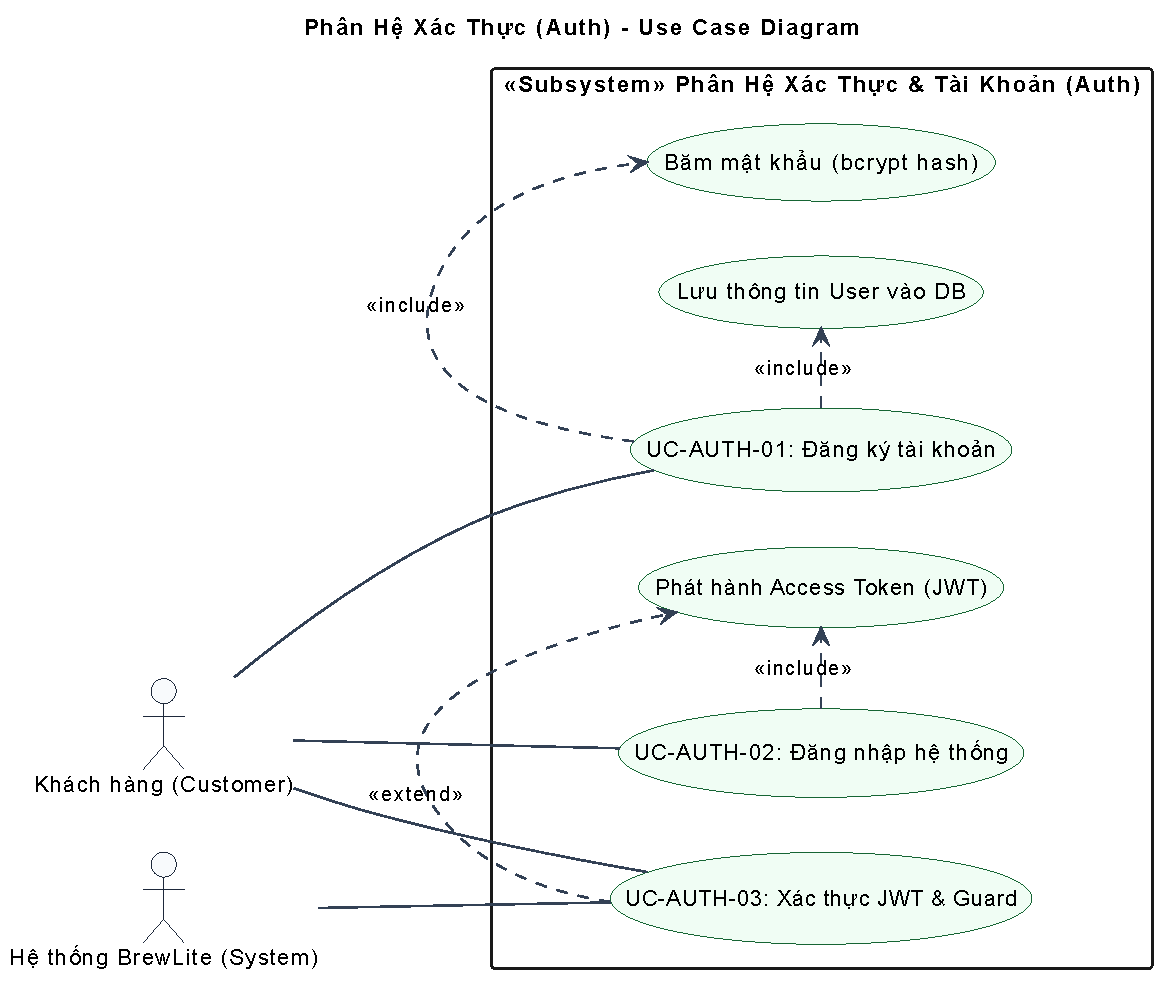
\includegraphics[width=0.75\textwidth]{figures/usecase-auth.pdf}
    \caption{Sơ đồ Use Case - Phân hệ Xác thực}
    \label{fig:usecase-auth}
\end{figure}

\begin{table}[H]
\centering
\small
\caption{Đặc tả Use Case: Đăng ký và Đăng nhập người dùng}
\label{tab:uc-spec-auth}
\begin{tabularx}{\textwidth}{p{2.3cm}XX}
\toprule
\textbf{Mục} & \textbf{Đăng ký (UC-AUTH-01)} & \textbf{Đăng nhập (UC-AUTH-02)} \\
\midrule
\textbf{Actor} & Khách vãng lai (Guest) & Khách hàng đã có tài khoản \\
\midrule
\textbf{Tiền điều kiện} & Chưa đăng nhập; địa chỉ email chưa tồn tại trên hệ thống. & Đã có tài khoản trên hệ thống; tài khoản ở trạng thái hoạt động. \\
\midrule
\textbf{Hậu điều kiện} & Bản ghi mới được tạo trong bảng \texttt{users}; mật khẩu được băm Bcrypt 10 rounds; khởi tạo 0 điểm loyalty. & Cấp phát mã thông báo JWT \texttt{accessToken}; lưu trữ tại client để xác thực các request kế tiếp. \\
\midrule
\textbf{Luồng chính} & 
1. Người dùng nhập email, mật khẩu (\(\ge\) 6 ký tự), họ tên.\newline
2. Nhấn "Đăng ký".\newline
3. Hệ thống kiểm tra hợp lệ DTO và tính duy nhất của email.\newline
4. Băm mật khẩu bằng \texttt{bcrypt.hash(password, 10)}.\newline
5. Tạo người dùng trong DB và trả về thông tin (loại trừ \texttt{password\_hash}). & 
1. Người dùng nhập email và mật khẩu.\newline
2. Nhấn "Đăng nhập".\newline
3. Hệ thống tìm người dùng theo email.\newline
4. So sánh mật khẩu bằng \texttt{bcrypt.compare(password, hash)}.\newline
5. Sinh mã JWT chứa payload \texttt{\{sub, email\}}.\newline
6. Trả về token và thông tin hồ sơ người dùng. \\
\midrule
\textbf{Luồng ngoại lệ} & 
- DTO không hợp lệ: Trả về mã \texttt{400 Bad Request}.\newline
- Trùng email: Trả về \texttt{409 Conflict} ("Email đã được sử dụng"). & 
- Email không tồn tại hoặc sai mật khẩu: Trả về \texttt{401 Unauthorized} ("Email hoặc mật khẩu không chính xác"). \\
\bottomrule
\end{tabularx}
\end{table}

\clearpage
\subsection{Sơ đồ Hoạt động (Activity Diagram)}
Sơ đồ Hoạt động mô tả chi tiết quy trình xử lý luồng đăng nhập và kiểm tra xác thực người dùng được biểu diễn tại Hình~\ref{fig:activity-auth}.

\begin{figure}[H]
    \centering
    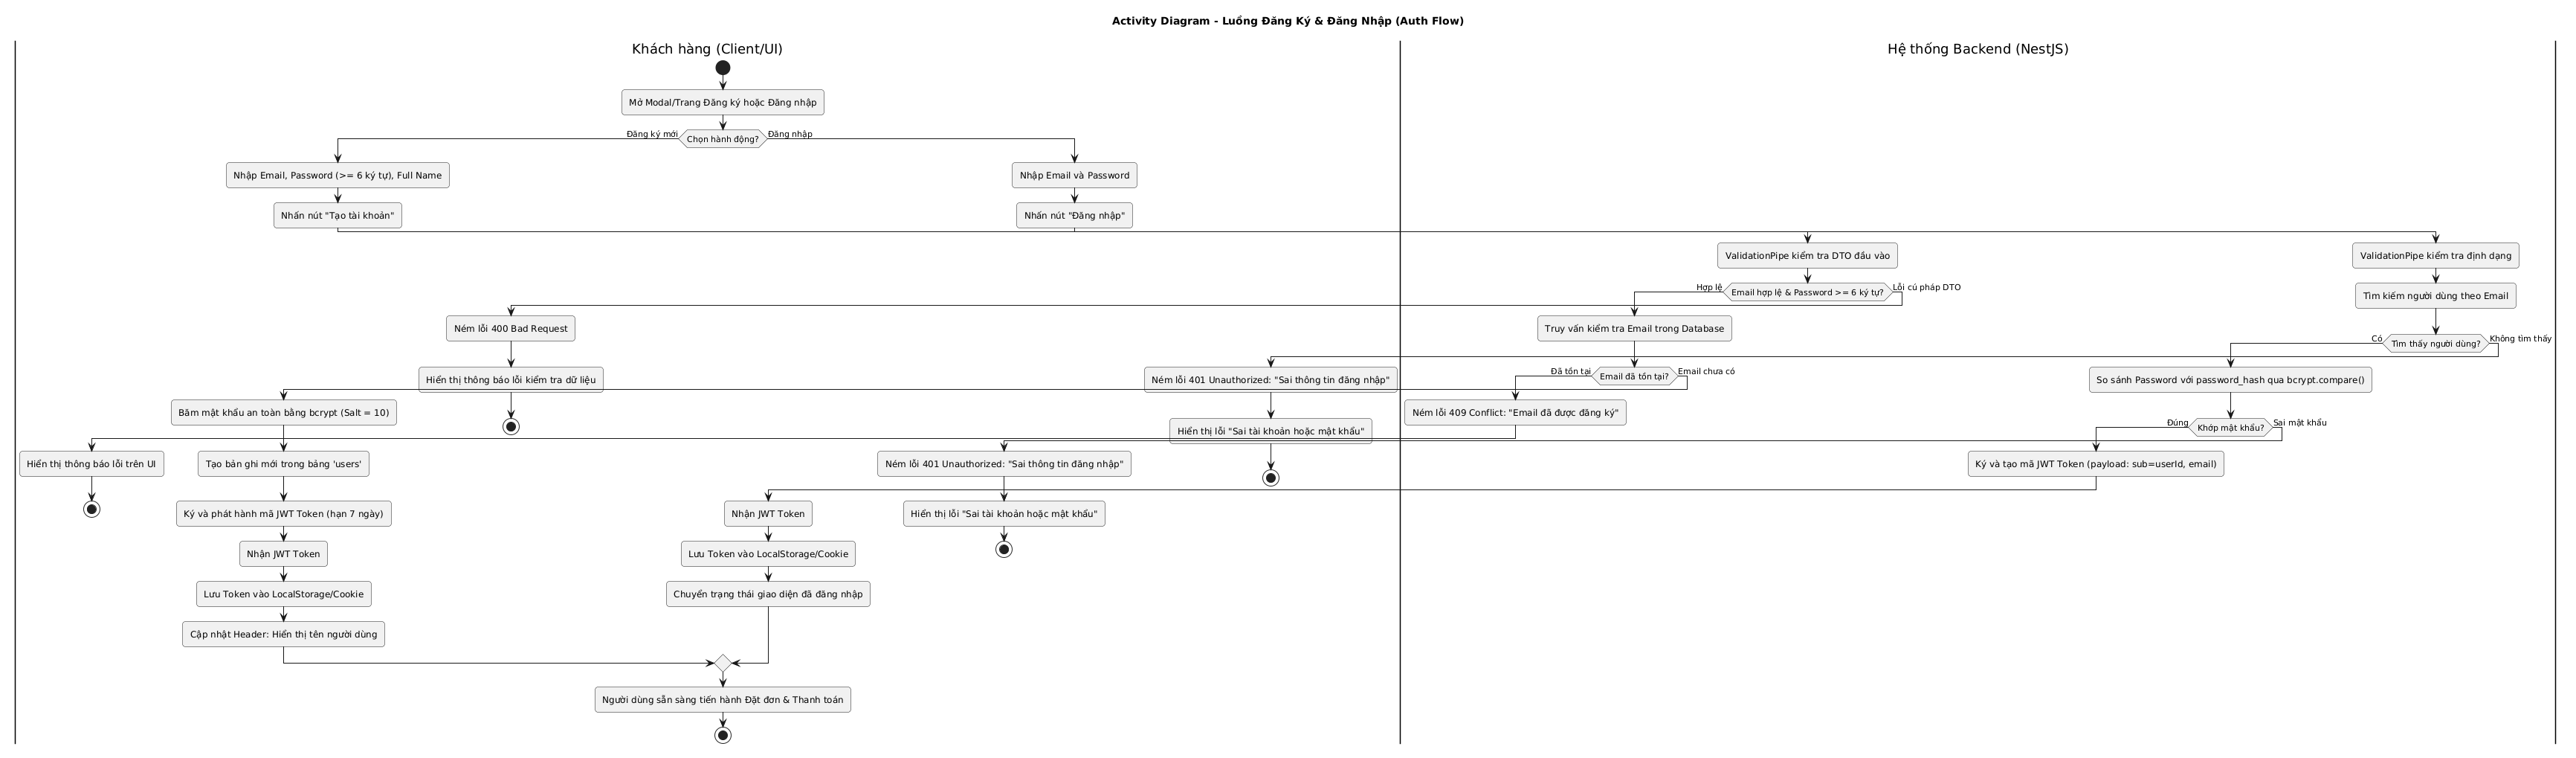
\includegraphics[width=\textwidth, height=0.82\textheight, keepaspectratio]{figures/activity-auth.png}
    \caption{Sơ đồ Hoạt động - Phân hệ Xác thực}
    \label{fig:activity-auth}
\end{figure}

\clearpage
\subsection{Sơ đồ Tuần tự (Sequence Diagram)}
Sơ đồ Tuần tự phản ánh chuẩn xác các lời gọi hàm từ giao diện qua Controller đến Service và Prisma DB tại Hình~\ref{fig:sequence-auth}.

\begin{figure}[H]
    \centering
    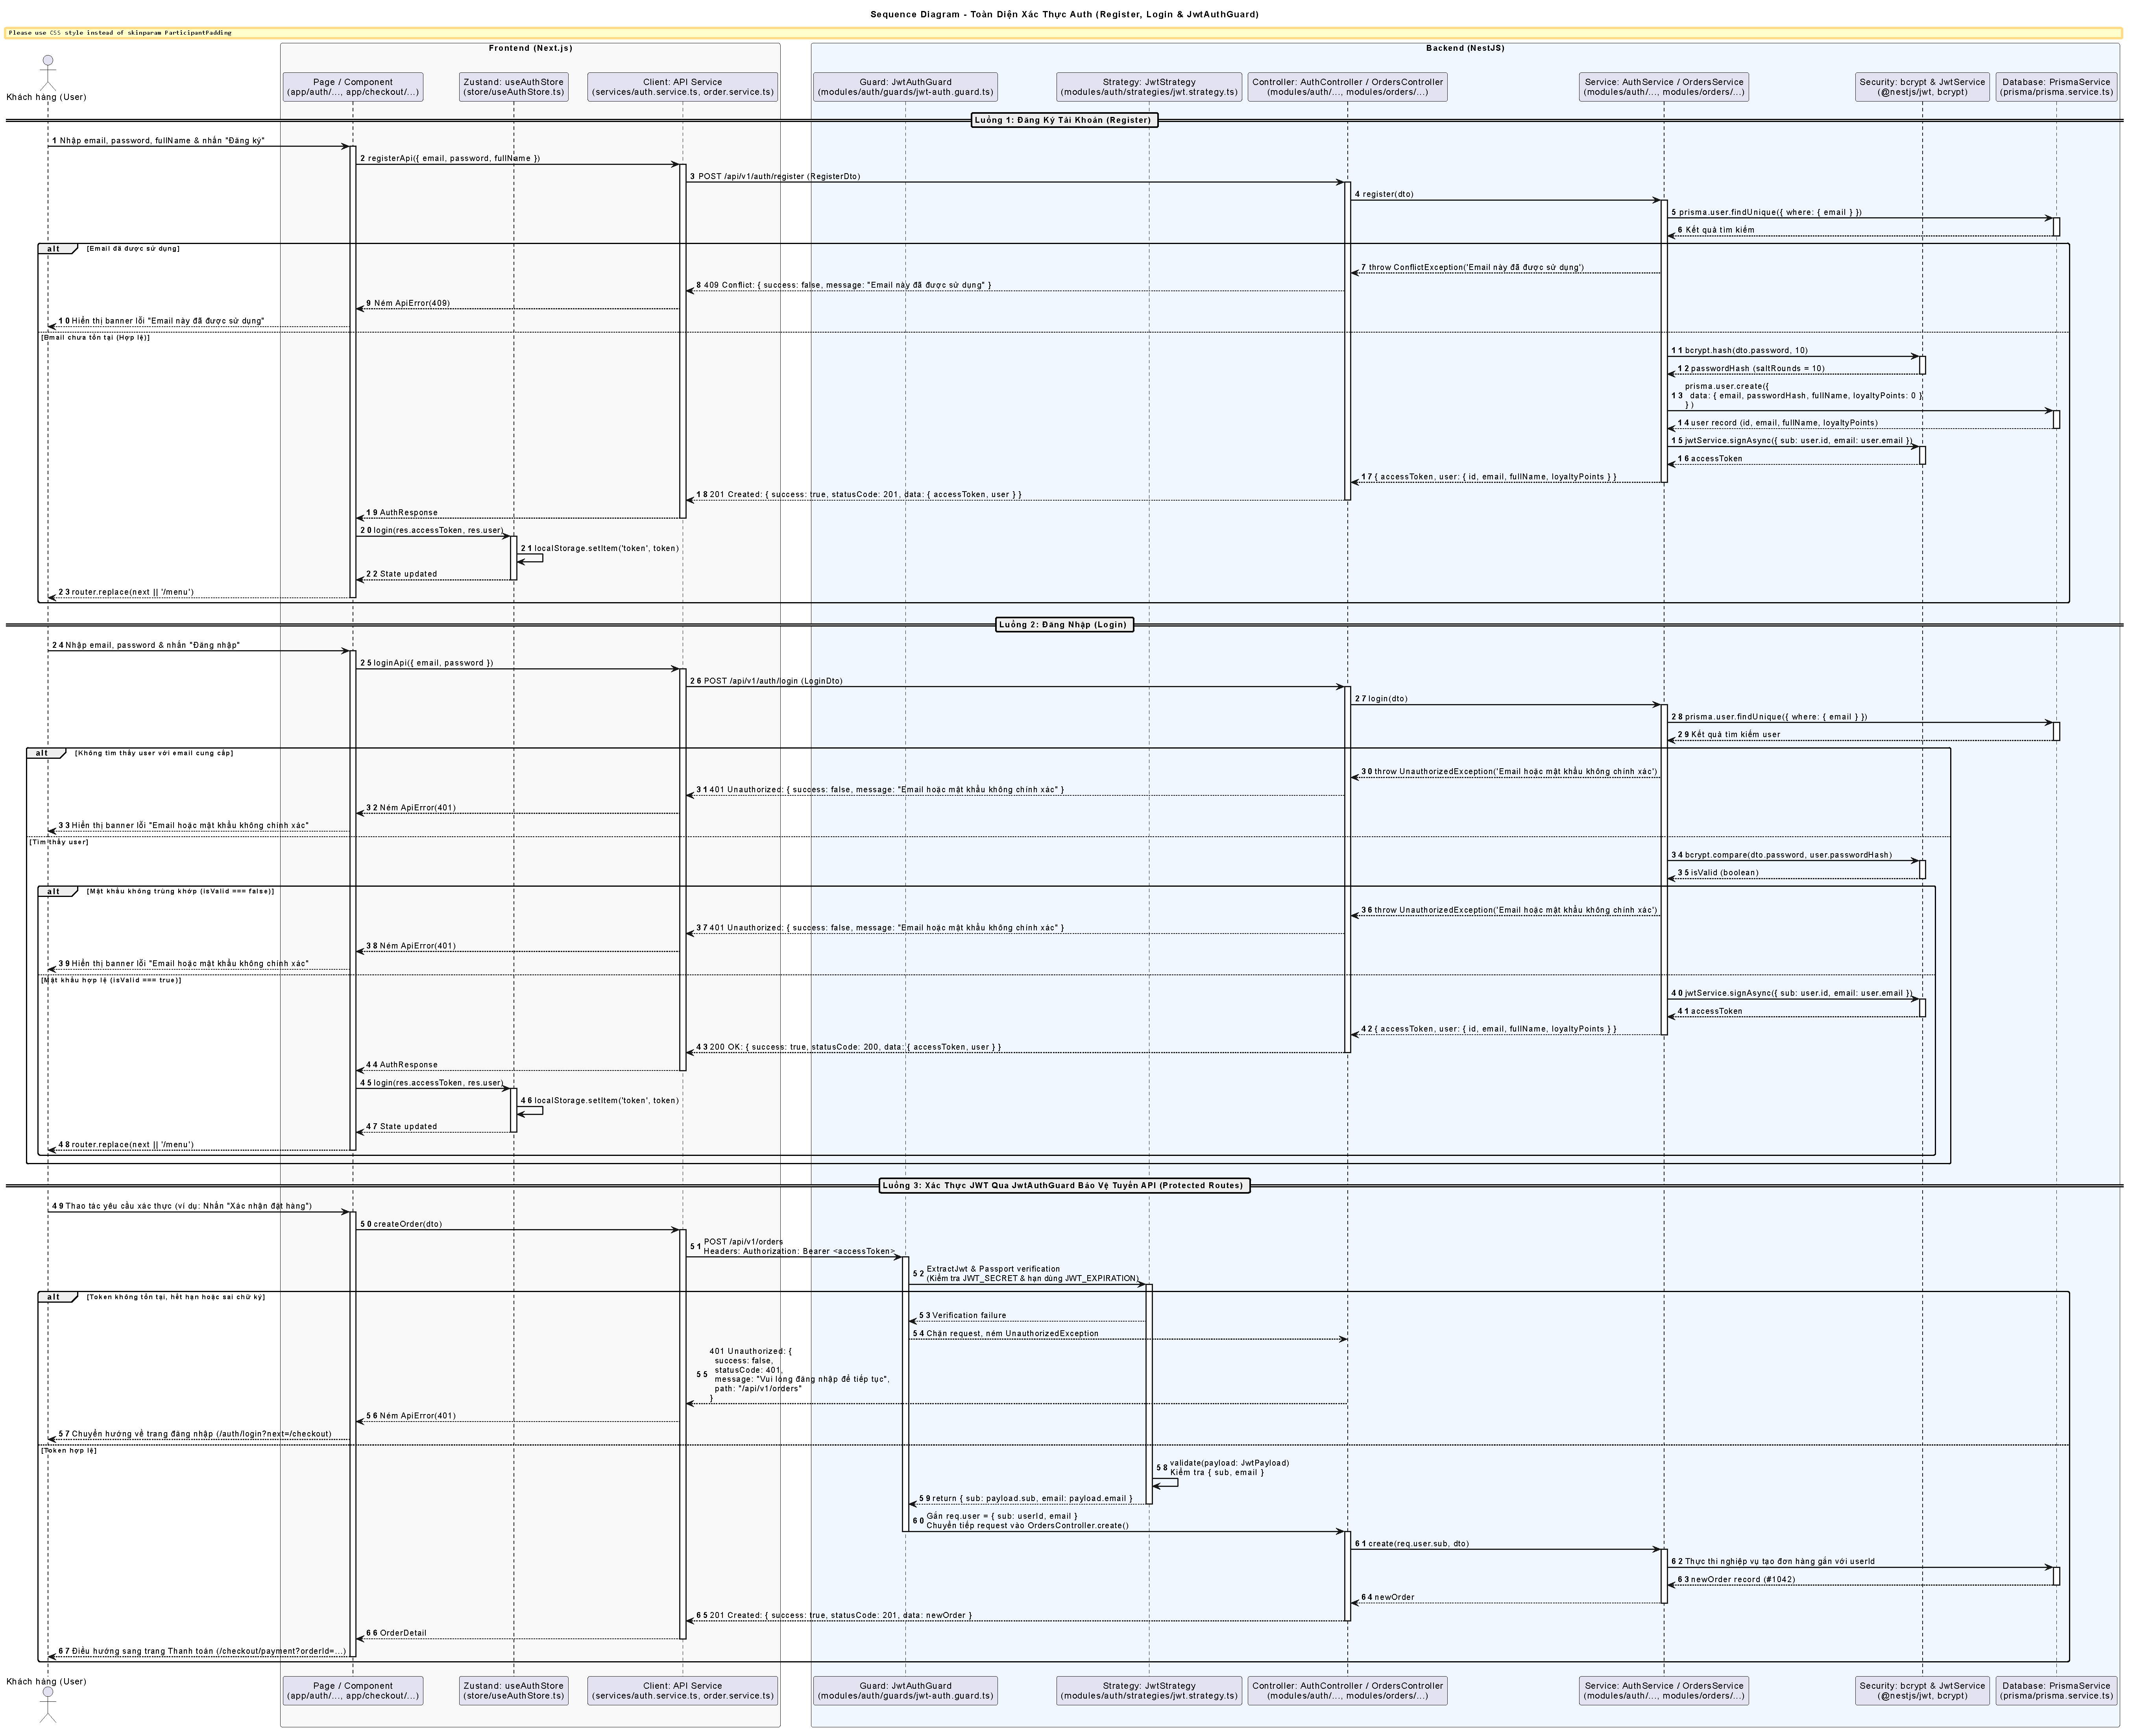
\includegraphics[width=\textwidth, height=0.82\textheight, keepaspectratio]{figures/sequence-auth.pdf}
    \caption{Sơ đồ Tuần tự - Phân hệ Xác thực (Happy path \& Exception paths)}
    \label{fig:sequence-auth}
\end{figure}

\clearpage
\subsection{Hợp đồng API (API Contract)}
\begin{table}[H]
\centering
\small
\caption{Danh mục API Endpoints - Phân hệ Xác thực}
\label{tab:api-auth}
\begin{tabularx}{\textwidth}{llp{4cm}X}
\toprule
\textbf{Phương thức} & \textbf{Endpoint} & \textbf{Mô tả Request Body} & \textbf{Phản hồi chính} \\
\midrule
\texttt{POST} & \texttt{/api/v1/auth/register} & \texttt{\{email, password, fullName\}} (Email hợp lệ, password \(\ge 6\) ký tự) & \texttt{201 Created}: Trả về thông tin người dùng mới (loại trừ passwordHash). Lỗi: \texttt{400}, \texttt{409}. \\
\texttt{POST} & \texttt{/api/v1/auth/login} & \texttt{\{email, password\}} & \texttt{200 OK}: Trả về \texttt{accessToken} và thông tin người dùng. Lỗi: \texttt{400}, \texttt{401}. \\
\bottomrule
\end{tabularx}
\end{table}

\subsection{Ánh xạ Cơ sở dữ liệu (Database Mapping)}
Mọi thao tác của AuthModule tác động trực tiếp lên bảng \texttt{users}:
\begin{itemize}
    \item \textbf{Đăng ký:} Gọi \texttt{prisma.user.findUnique(\{ where: \{ email \} \})}. Nếu tồn tại \(\to\) throw \texttt{ConflictException}. Nếu chưa, thực thi \texttt{bcrypt.hash(password, 10)} và gọi \texttt{prisma.user.create(\{ data: \{ email, passwordHash, fullName, loyaltyPoints: 0 \} \})}.
    \item \textbf{Đăng nhập:} Gọi \texttt{prisma.user.findUnique(\{ where: \{ email \} \})}. Nếu không tìm thấy hoặc \texttt{bcrypt.compare()} trả về false \(\to\) throw \texttt{UnauthorizedException}.
    \item \textbf{Bảo mật dữ liệu:} Trường \texttt{passwordHash} tuyệt đối được lược bỏ trước khi gán vào đối tượng trả về thông qua destructuring: \texttt{const \{ passwordHash, ...userWithoutPassword \} = user}.
\end{itemize}

\subsection{Kịch bản Kiểm thử (Test Cases)}
\begin{table}[H]
\centering
\small
\caption{Tóm lược các Ca kiểm thử tiêu biểu - Phân hệ Xác thực}
\label{tab:tc-auth}
\begin{tabularx}{\textwidth}{llp{2.6cm}p{3cm}Xc}
\toprule
\textbf{Mã TC} & \textbf{Loại} & \textbf{Tiền điều kiện} & \textbf{Endpoint / Màn hình} & \textbf{Kết quả mong đợi} & \textbf{Trạng thái} \\
\midrule
\texttt{TC-AUTH-API-01} & Hợp lệ & Email chưa tồn tại & \texttt{POST /auth/register} & HTTP 201, tạo user mới, băm bcrypt 10 rounds & Chưa chạy \\
\texttt{TC-AUTH-API-03} & Lỗi & Email đã tồn tại & \texttt{POST /auth/register} & HTTP 409, message "Email đã được sử dụng" & Chưa chạy \\
\texttt{TC-AUTH-API-05} & Hợp lệ & Đã có tài khoản & \texttt{POST /auth/login} & HTTP 200, cấp JWT accessToken & Chưa chạy \\
\texttt{TC-AUTH-API-07} & Lỗi & Mật khẩu không đúng & \texttt{POST /auth/login} & HTTP 401, message "Email hoặc mật khẩu không chính xác" & Chưa chạy \\
\texttt{TC-AUTH-UI-01} & Giao diện & Đang ở trang \texttt{/login} & Màn hình Đăng nhập & Hiển thị form, nút "Đăng nhập", chuyển hướng thành công & Chưa chạy \\
\bottomrule
\end{tabularx}
\end{table}

\subsection{Giao diện Người dùng}
\begin{figure}[H]
    \centering
    \begin{subfigure}[b]{0.48\textwidth}
        \centering
        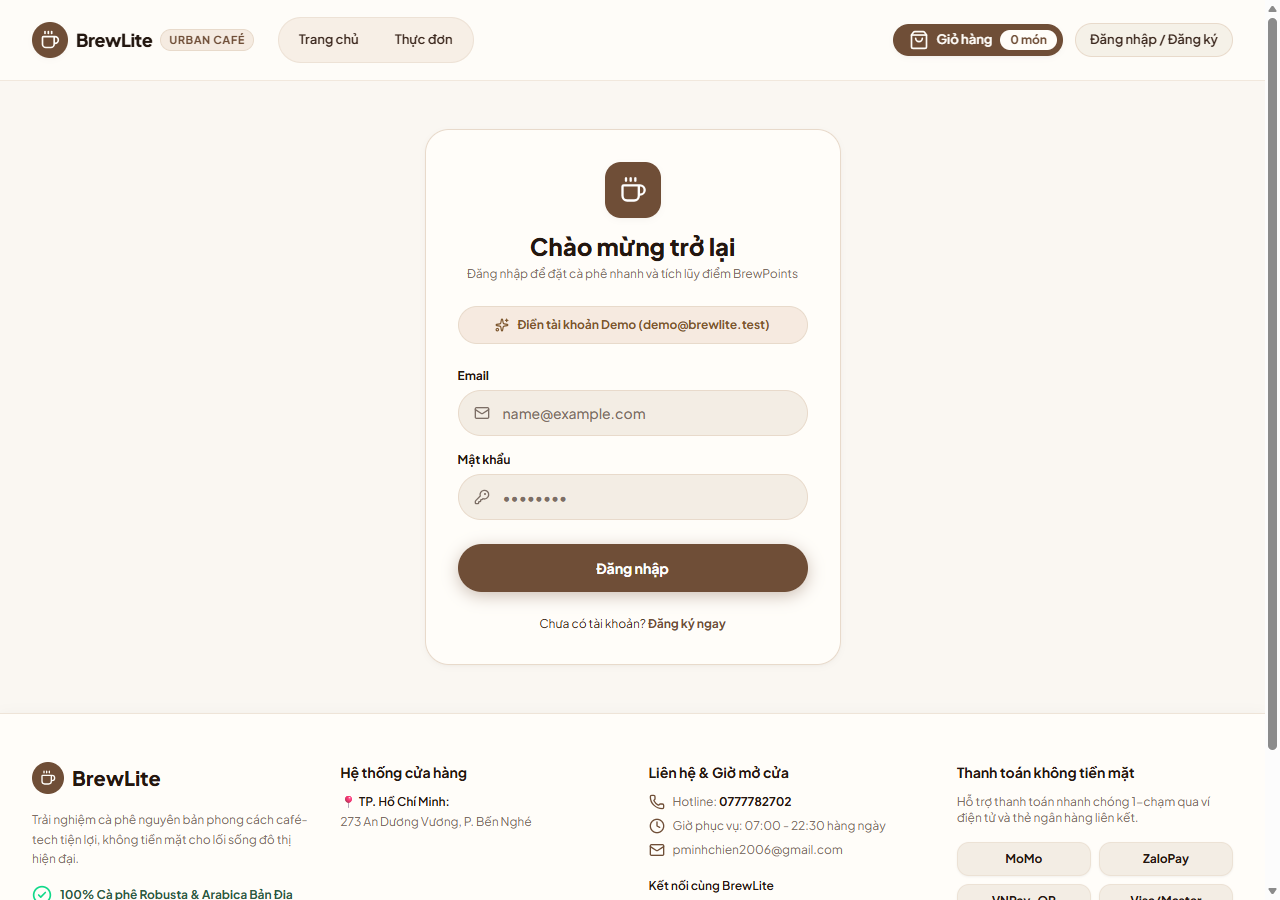
\includegraphics[width=\textwidth]{figures/ui-auth-login.png}
        \caption{Màn hình Đăng nhập}
        \label{fig:ui-auth-login}
    \end{subfigure}
    \hfill
    \begin{subfigure}[b]{0.48\textwidth}
        \centering
        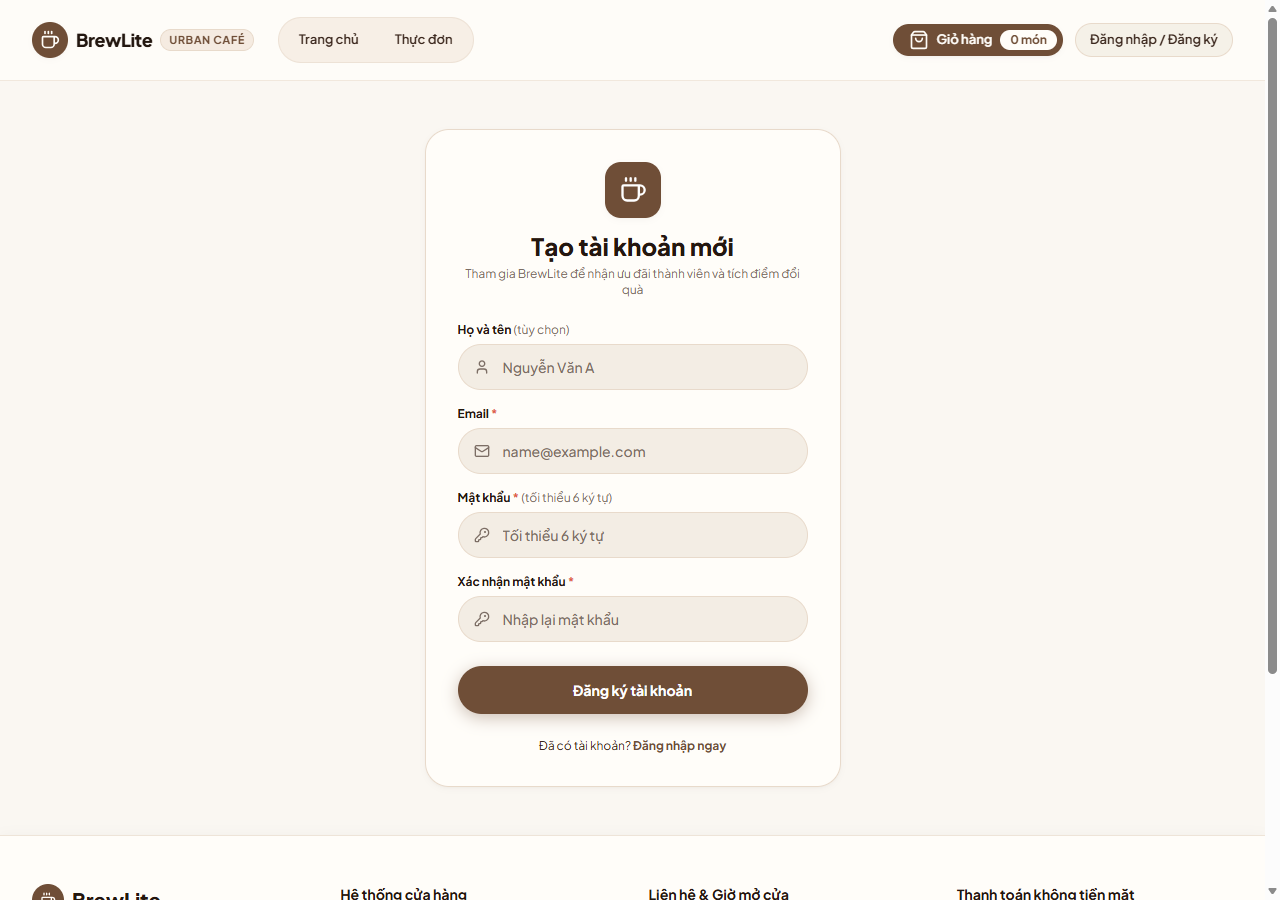
\includegraphics[width=\textwidth]{figures/ui-auth-register.png}
        \caption{Màn hình Đăng ký tài khoản}
        \label{fig:ui-auth-register}
    \end{subfigure}
    \caption{Giao diện Đăng nhập và Đăng ký người dùng}
    \label{fig:ui-auth}
\end{figure}

% ====== END INLINE: chapters/feature-auth ======


% ====== BEGIN INLINE: chapters/feature-catalog ======
\clearpage
\section{Phân hệ Danh mục Sản phẩm (Product Catalog)}

\subsection{Đặc tả Use Case}
Phân hệ Danh mục Sản phẩm cho phép người dùng khám phá toàn bộ thực đơn của BrewLite, tìm kiếm đồ uống theo tên và lọc theo các phân loại như Cà phê hoặc Trà. Sơ đồ Use Case được biểu diễn tại Hình~\ref{fig:usecase-product-catalog}.

\begin{figure}[H]
    \centering
    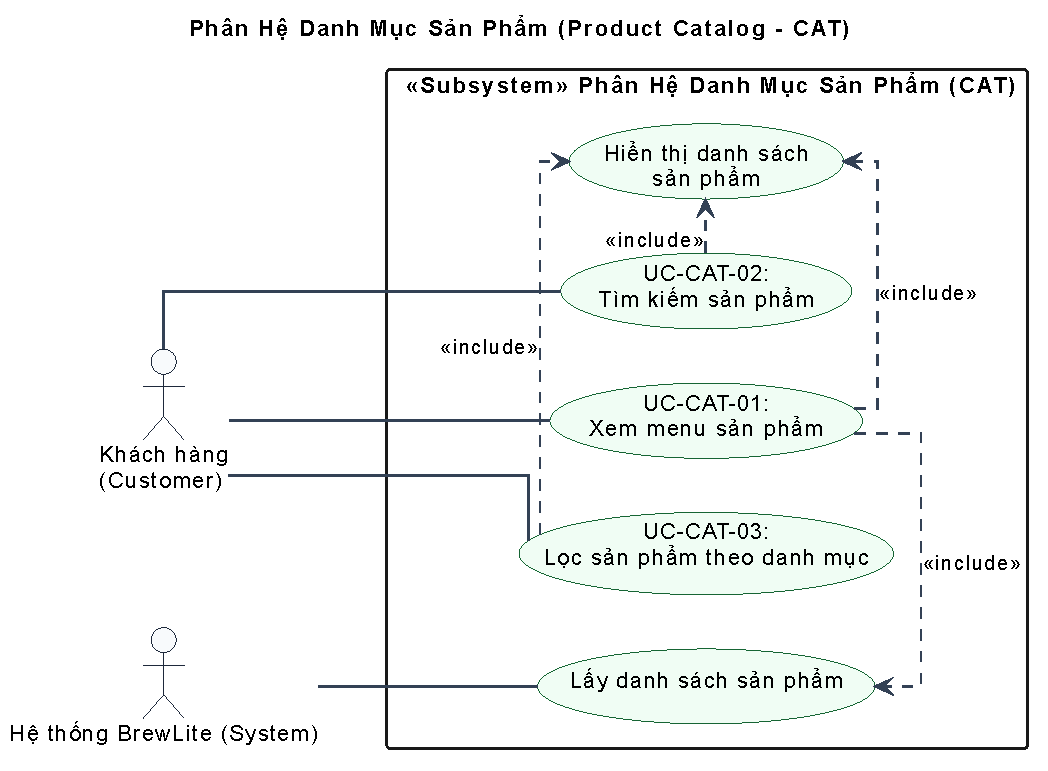
\includegraphics[width=0.75\textwidth]{figures/usecase-product-catalog.pdf}
    \caption{Sơ đồ Use Case - Phân hệ Danh mục Sản phẩm}
    \label{fig:usecase-product-catalog}
\end{figure}

\begin{table}[H]
\centering
\small
\caption{Đặc tả Use Case: Xem và Tìm kiếm Danh mục Sản phẩm (UC-CAT-01)}
\label{tab:uc-spec-catalog}
\begin{tabularx}{\textwidth}{p{2.8cm}X}
\toprule
\textbf{Mục} & \textbf{Chi tiết Đặc tả} \\
\midrule
\textbf{Actor} & Khách vãng lai, Khách hàng đăng nhập \\
\midrule
\textbf{Tiền điều kiện} & Hệ thống có dữ liệu sản phẩm và danh mục đã được kích hoạt trong CSDL. \\
\midrule
\textbf{Hậu điều kiện} & Danh sách sản phẩm tương ứng hiển thị trực quan trên giao diện thực đơn. \\
\midrule
\textbf{Luồng chính} & 
1. Người dùng truy cập trang Thực đơn (\texttt{/products}).\newline
2. Giao diện gửi request \texttt{GET /api/v1/categories} và \texttt{GET /api/v1/products}.\newline
3. Hệ thống trả về danh sách danh mục (Cà phê, Trà) và danh sách 10 sản phẩm (6 món cà phê, 4 món trà theo seed data).\newline
4. Khách hàng nhấp chọn tab phân loại (ví dụ "Cà phê") hoặc nhập từ khóa tìm kiếm (ví dụ "Latte").\newline
5. Hook \texttt{useProductCatalog} lọc lại danh sách hiển thị tương ứng kèm nhãn giá cơ bản và trạng thái còn hàng/hết hàng. \\
\midrule
\textbf{Luồng ngoại lệ} & 
- Lỗi kết nối mạng hoặc máy chủ backend: Hiển thị thông báo tải dữ liệu thất bại và cung cấp nút thử lại.\newline
- Không tìm thấy sản phẩm phù hợp: Hiển thị thông báo "Không tìm thấy sản phẩm nào phù hợp". \\
\bottomrule
\end{tabularx}
\end{table}

\clearpage
\subsection{Sơ đồ Hoạt động (Activity Diagram)}
Quy trình nạp và lọc danh mục sản phẩm được mô tả tại Hình~\ref{fig:activity-product-catalog}.

\begin{figure}[H]
    \centering
    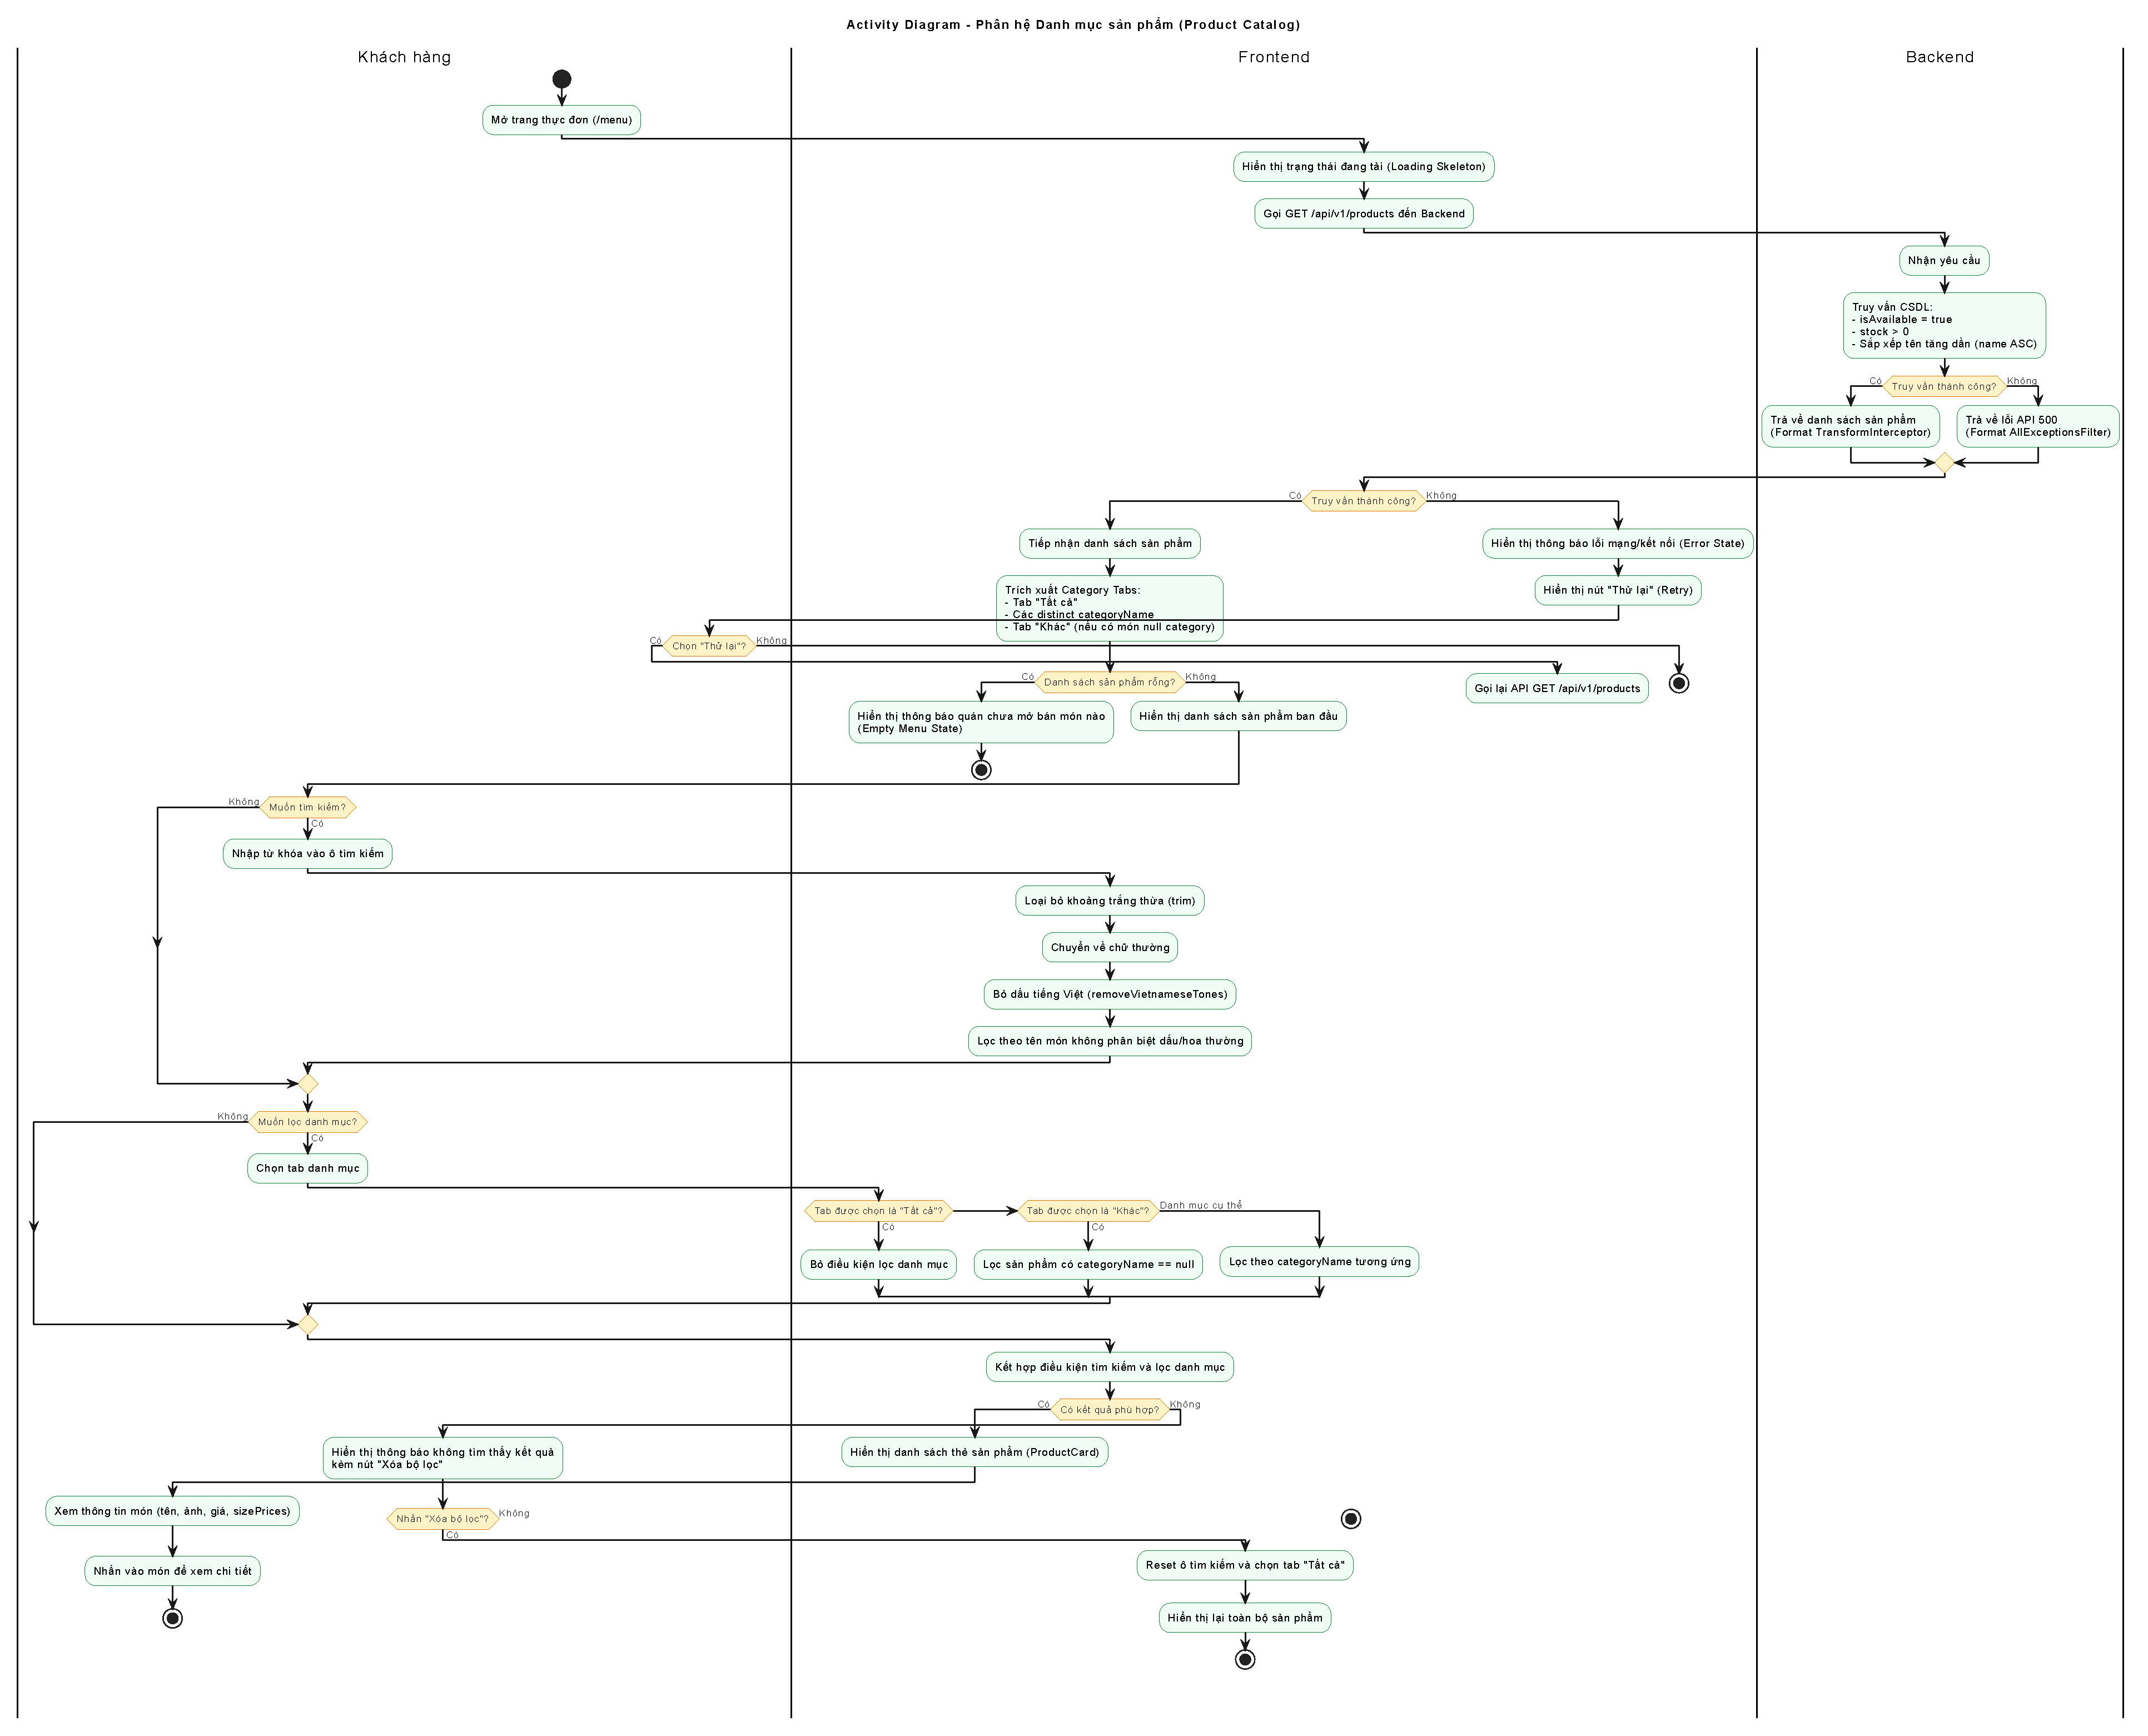
\includegraphics[width=\textwidth, height=0.98\textheight, keepaspectratio]{figures/activity-product-catalog.pdf}
    \caption{Sơ đồ Hoạt động - Phân hệ Danh mục Sản phẩm}
    \label{fig:activity-product-catalog}
\end{figure}

\clearpage
\subsection{Sơ đồ Tuần tự (Sequence Diagram)}
Sơ đồ Tuần tự phản ánh quá trình truy vấn danh mục và sản phẩm từ Frontend đến Backend Controller, Service và Prisma tại Hình~\ref{fig:sequence-product-catalog}.

\begin{figure}[H]
    \centering
    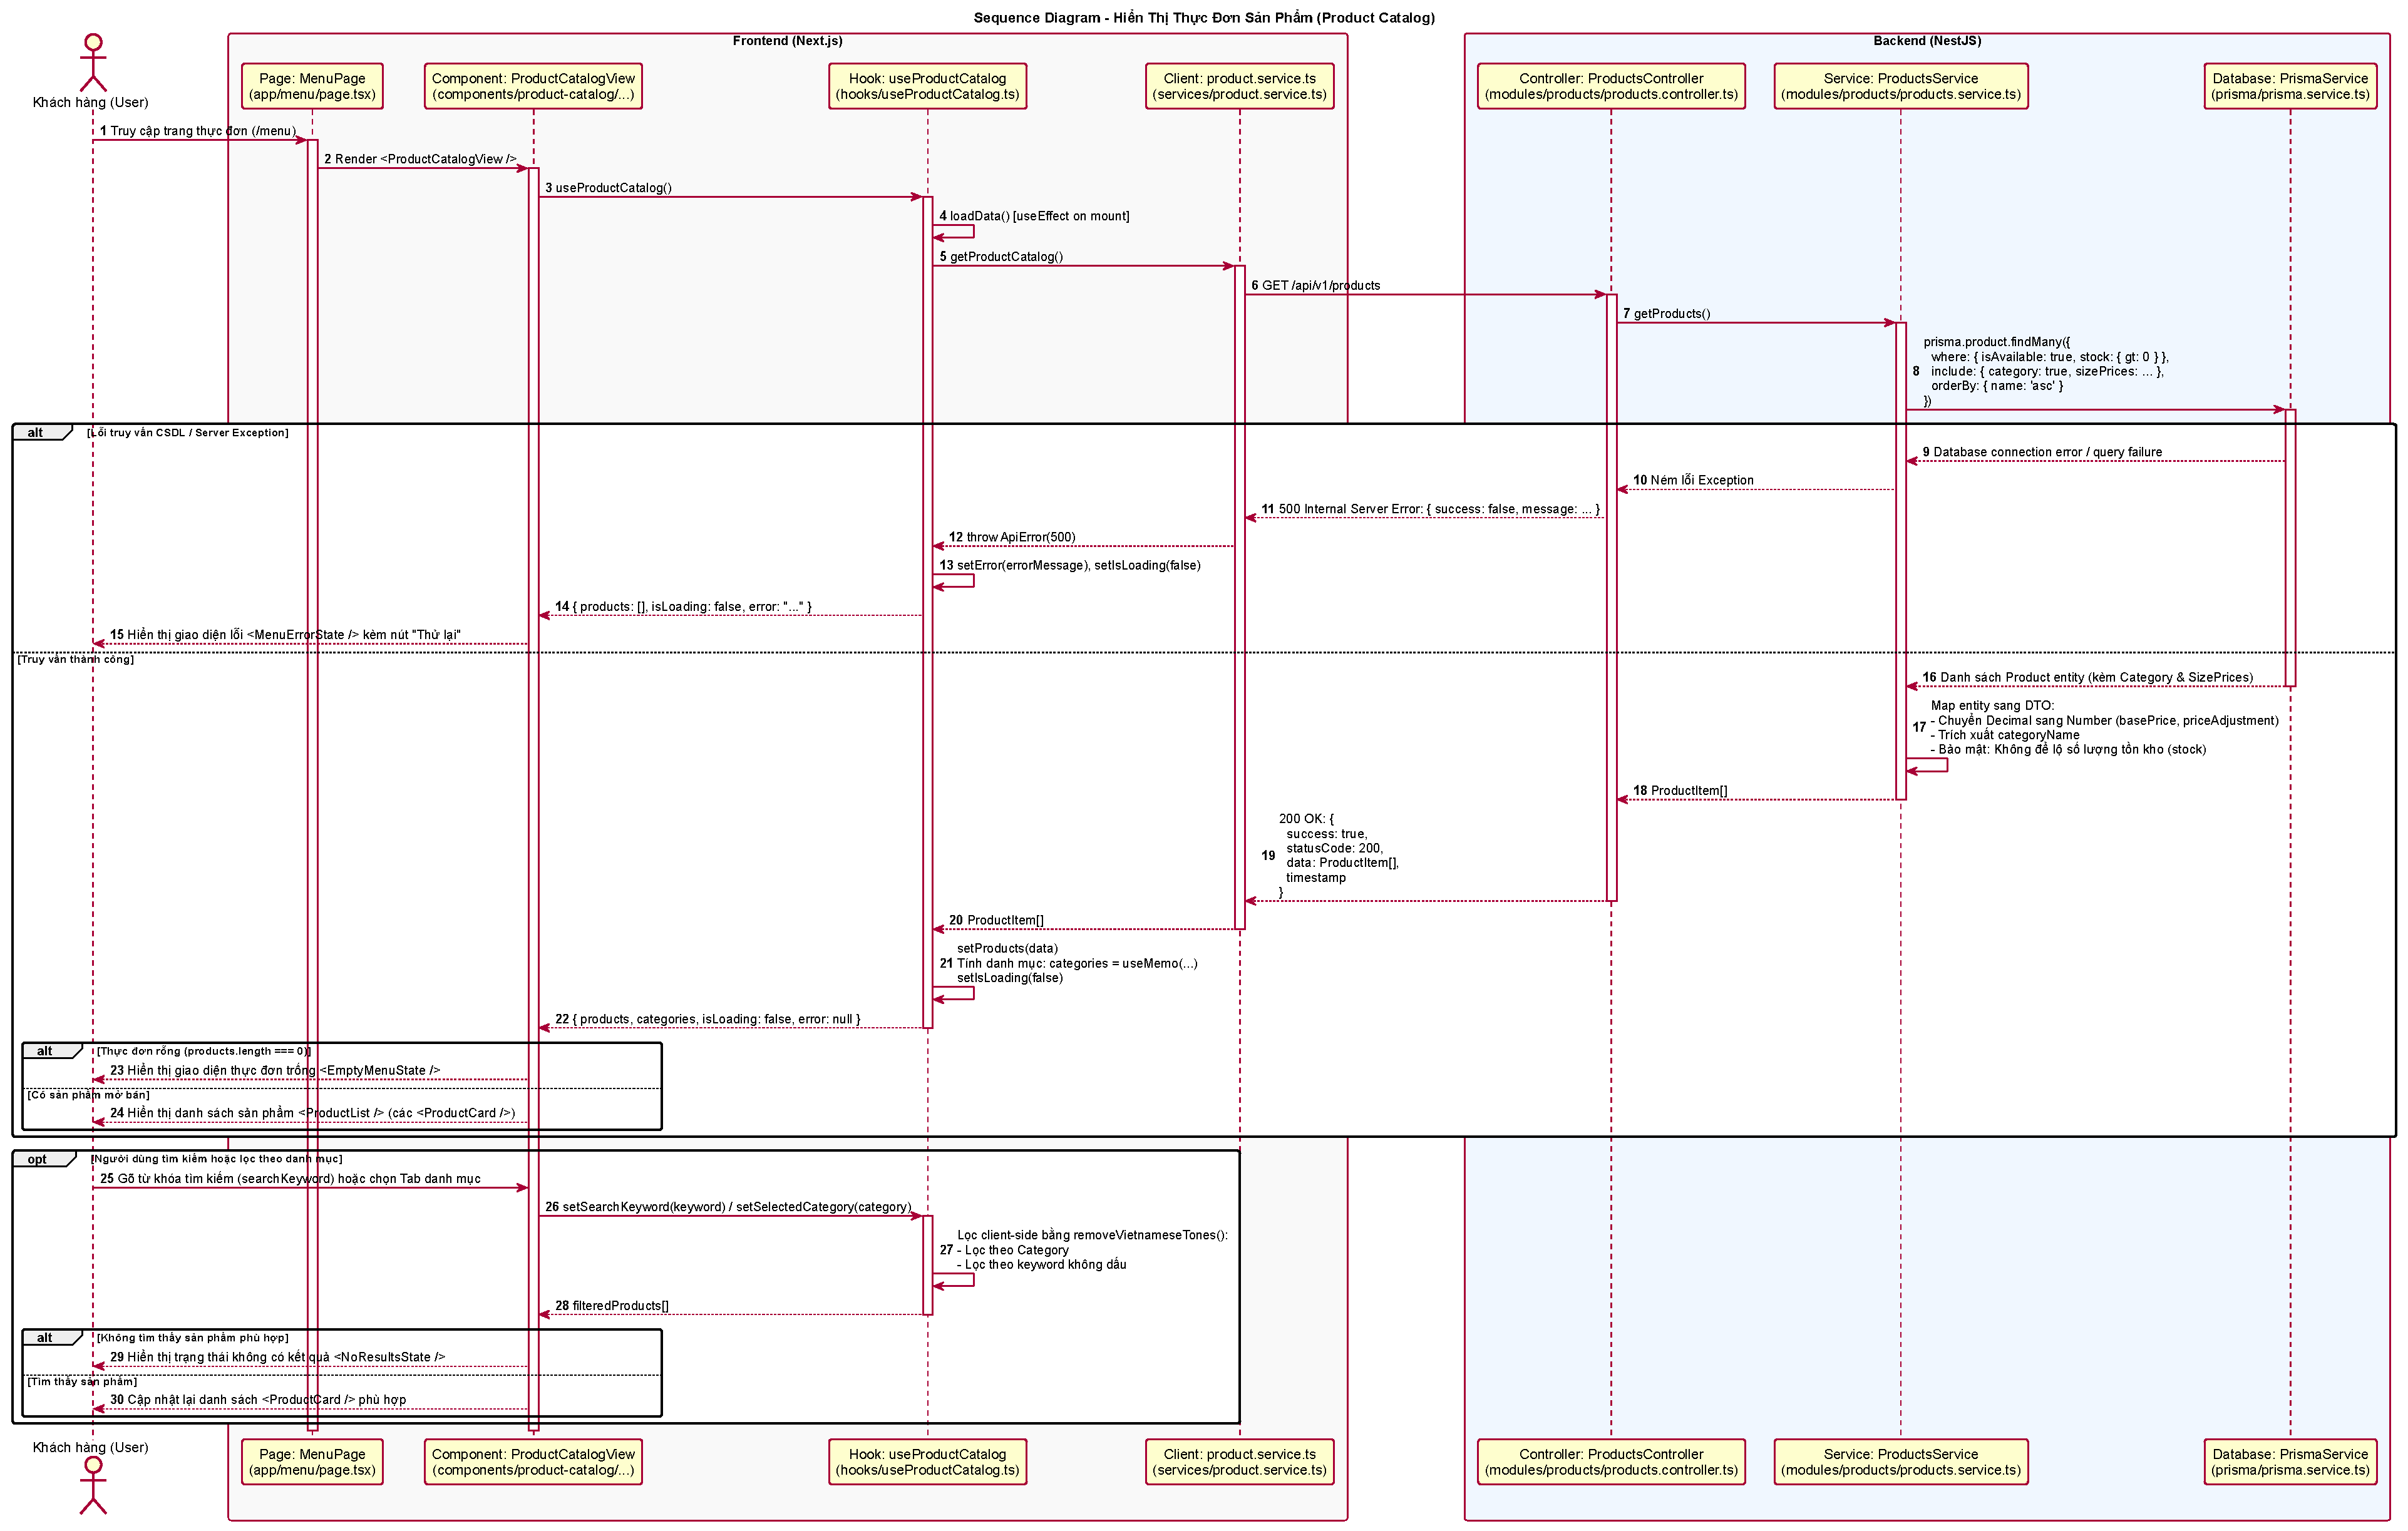
\includegraphics[width=\textwidth, height=0.80\textheight, keepaspectratio]{figures/sequence-product-catalog.pdf}
    \caption{Sơ đồ Tuần tự - Phân hệ Danh mục Sản phẩm}
    \label{fig:sequence-product-catalog}
\end{figure}

\clearpage
\subsection{Hợp đồng API (API Contract)}
\begin{table}[H]
\centering
\small
\caption{Danh mục API Endpoints - Phân hệ Danh mục Sản phẩm}
\label{tab:api-catalog}
\begin{tabularx}{\textwidth}{llp{4cm}X}
\toprule
\textbf{Phương thức} & \textbf{Endpoint} & \textbf{Tham số Query} & \textbf{Phản hồi chính} \\
\midrule
\texttt{GET} & \texttt{/api/v1/categories} & Không có & \texttt{200 OK}: Danh sách danh mục sắp xếp theo \texttt{displayOrder} tăng dần. \\
\texttt{GET} & \texttt{/api/v1/products} & \texttt{categoryId}, \texttt{search}, \texttt{availableOnly} & \texttt{200 OK}: Danh sách sản phẩm kèm thông tin giá cơ bản, hình ảnh và trạng thái khả dụng. \\
\bottomrule
\end{tabularx}
\end{table}

\subsection{Ánh xạ Cơ sở dữ liệu (Database Mapping)}
\begin{itemize}
    \item Truy vấn danh mục: \texttt{prisma.category.findMany(\{ orderBy: \{ displayOrder: 'asc' \} \})}.
    \item Truy vấn sản phẩm: \texttt{prisma.product.findMany(\{ where: \{ ...filter \}, include: \{ sizePrices: true, category: true \} \})}.
    \item Dữ liệu seed chuẩn gồm 2 danh mục chính ("Cà phê" - 6 món, "Trà" - 4 món), tổng cộng 10 sản phẩm mẫu được nạp vào bảng \texttt{categories} và \texttt{products}.
\end{itemize}

\subsection{Kịch bản Kiểm thử (Test Cases)}
\begin{table}[H]
\centering
\small
\caption{Tóm lược các Ca kiểm thử tiêu biểu - Phân hệ Danh mục}
\label{tab:tc-catalog}
\begin{tabularx}{\textwidth}{llp{2.6cm}p{3cm}Xc}
\toprule
\textbf{Mã TC} & \textbf{Loại} & \textbf{Tiền điều kiện} & \textbf{Endpoint / Màn hình} & \textbf{Kết quả mong đợi} & \textbf{Trạng thái} \\
\midrule
\texttt{TC-CAT-API-01} & Hợp lệ & DB có 2 danh mục & \texttt{GET /categories} & Trả về đủ 2 danh mục "Cà phê", "Trà" & Chưa chạy \\
\texttt{TC-CAT-API-02} & Hợp lệ & DB có 10 sản phẩm & \texttt{GET /products} & Trả về danh sách 10 món kèm \texttt{basePrice} & Chưa chạy \\
\texttt{TC-CAT-UI-01} & Giao diện & Trang \texttt{/products} & Thực đơn chính & Hiển thị tab "Tất cả", "Cà phê", "Trà" & Chưa chạy \\
\texttt{TC-CAT-UI-07} & Giao diện & Chọn tab "Cà phê" & Lọc danh mục & Hiển thị đúng 6 món cà phê từ seed data & Chưa chạy \\
\bottomrule
\end{tabularx}
\end{table}

\subsection{Giao diện Người dùng}
\begin{figure}[H]
    \centering
    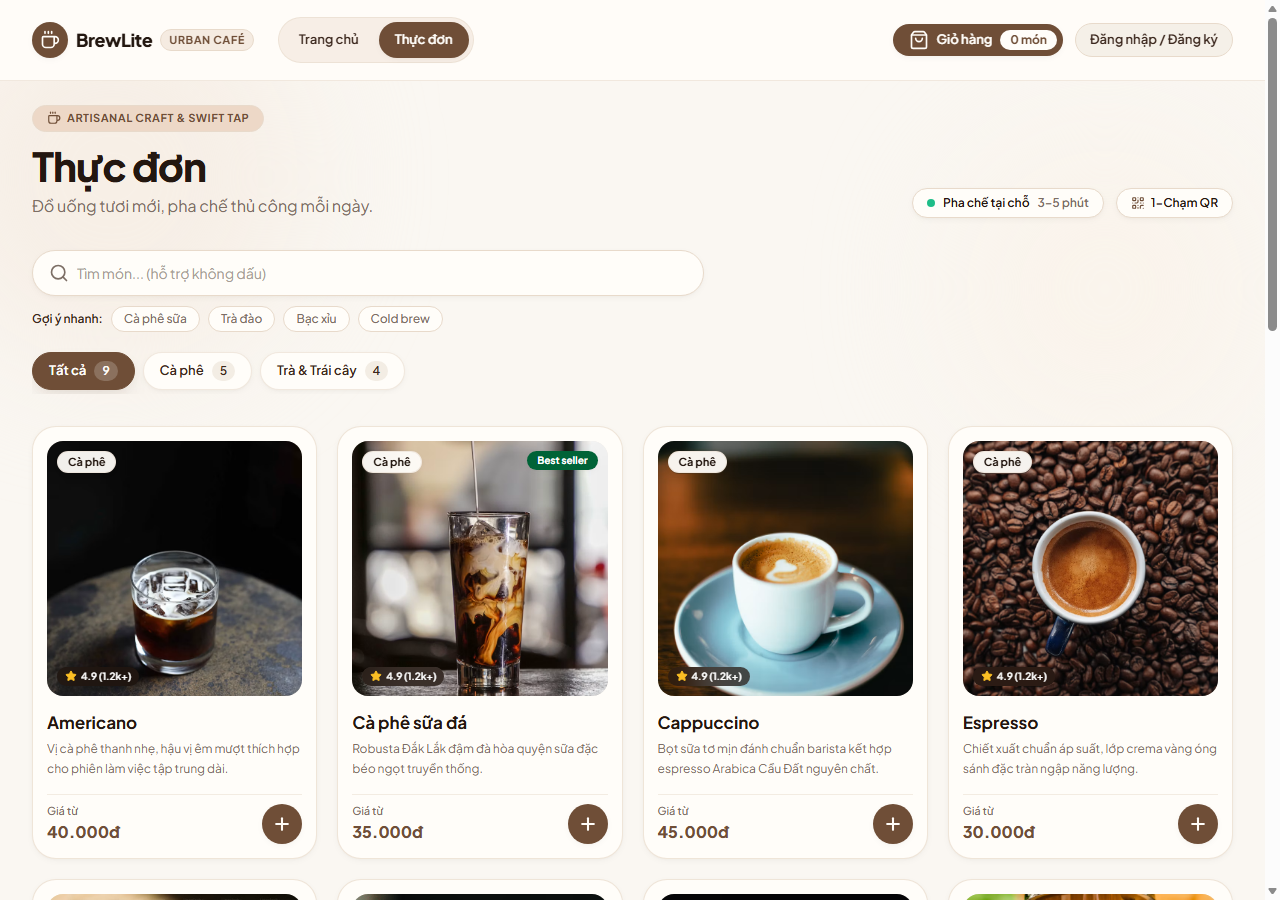
\includegraphics[width=0.92\textwidth]{figures/ui-catalog.png}
    \caption{Giao diện Thực đơn sản phẩm và Bộ lọc danh mục BrewLite}
    \label{fig:ui-catalog}
\end{figure}

% ====== END INLINE: chapters/feature-catalog ======


% ====== BEGIN INLINE: chapters/feature-detail ======
\clearpage
\section{Phân hệ Chi tiết Sản phẩm (Product Detail)}

\subsection{Đặc tả Use Case}
Phân hệ Chi tiết Sản phẩm cung cấp thông tin toàn diện về đồ uống, bao gồm mô tả, thành phần dinh dưỡng/nguyên liệu và cho phép khách hàng cá nhân hóa món đồ uống theo sở thích cá nhân. Sơ đồ Use Case được minh họa tại Hình~\ref{fig:usecase-product-detail}.

\begin{figure}[H]
    \centering
    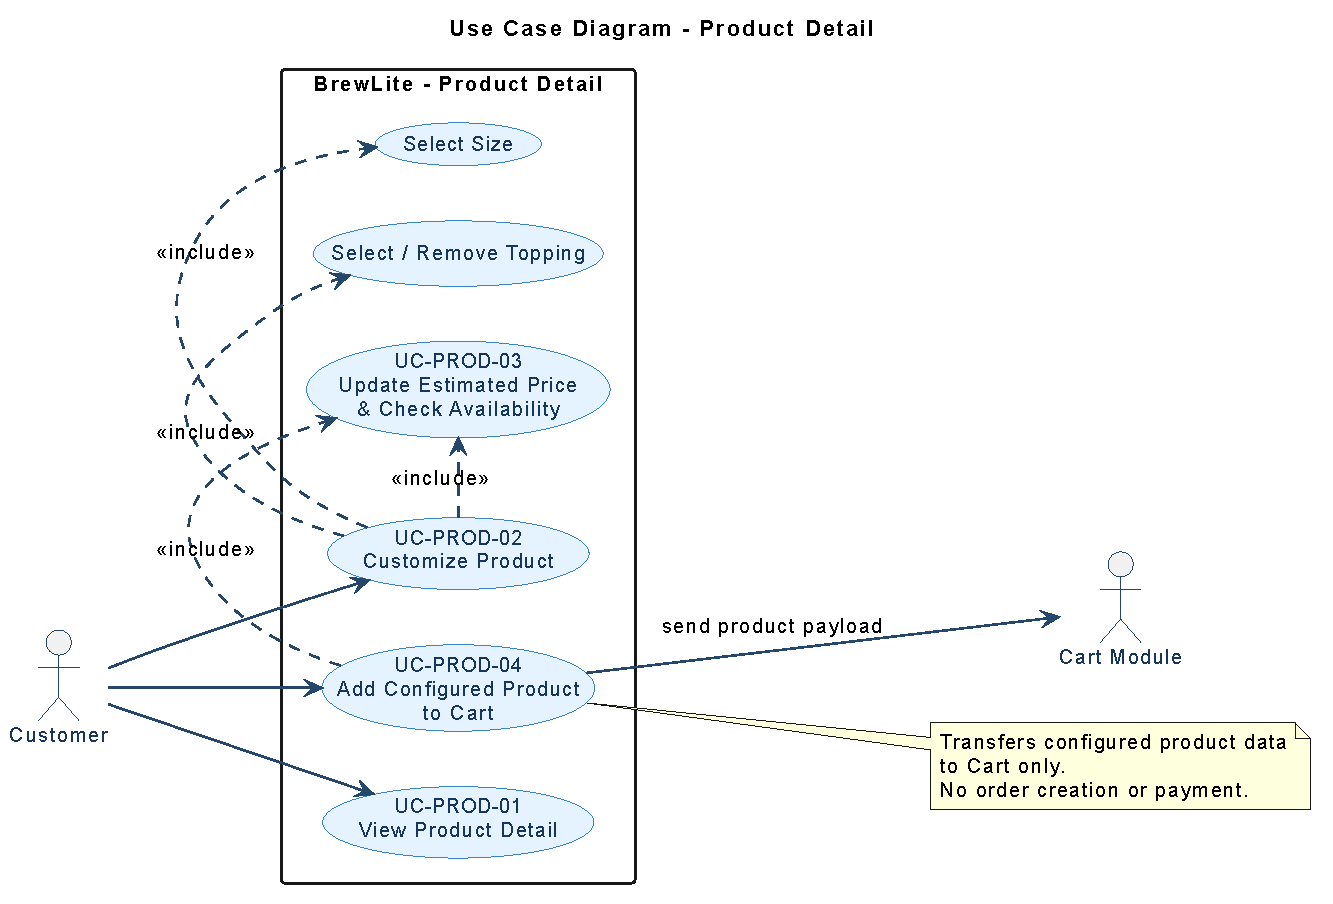
\includegraphics[width=0.75\textwidth]{figures/usecase-product-detail.pdf}
    \caption{Sơ đồ Use Case - Phân hệ Chi tiết Sản phẩm}
    \label{fig:usecase-product-detail}
\end{figure}

\begin{table}[H]
\centering
\small
\caption{Đặc tả Use Case: Xem chi tiết và Tùy biến món (UC-DET-01)}
\label{tab:uc-spec-detail}
\begin{tabularx}{\textwidth}{p{2.8cm}X}
\toprule
\textbf{Mục} & \textbf{Chi tiết Đặc tả} \\
\midrule
\textbf{Actor} & Khách vãng lai, Khách hàng đăng nhập \\
\midrule
\textbf{Tiền điều kiện} & Sản phẩm tồn tại trên hệ thống và có trạng thái \texttt{is\_available = true}. \\
\midrule
\textbf{Hậu điều kiện} & Thông tin món, các lựa chọn kích cỡ, mức ngọt, mức đá, danh sách topping và đơn giá tính toán động hiển thị đầy đủ trên màn hình. \\
\midrule
\textbf{Luồng chính} & 
1. Khách hàng nhấp vào thẻ món tại trang thực đơn.\newline
2. Trình duyệt điều hướng sang \texttt{/products/[id]}.\newline
3. Frontend gọi đồng thời \texttt{GET /api/v1/products/:id} và \texttt{GET /api/v1/toppings}.\newline
4. Giao diện hiển thị: tên món, hình ảnh, nút "Quay lại thực đơn", lựa chọn Size (Mặc định: M), mức đường (0\%, 30\%, 50\%, 70\%, 100\%), mức đá (0\%, 30\%, 50\%, 70\%, 100\%) và danh sách Topping kèm giá phụ thu.\newline
5. Khi người dùng thay đổi kích cỡ hoặc chọn thêm topping, giao diện tự động tính lại tổng đơn giá của món ăn theo thời gian thực.\newline
6. Khách hàng nhấn "Thêm vào giỏ hàng" để lưu món vào giỏ. \\
\midrule
\textbf{Luồng ngoại lệ} & 
- Sản phẩm không tồn tại: API trả về mã lỗi \texttt{404 Not Found}, giao diện hiển thị thông báo sản phẩm không tìm thấy và nút quay về thực đơn.\newline
- Sản phẩm hết hàng (\texttt{stock = 0}): Nút "Thêm vào giỏ hàng" bị vô hiệu hóa (\texttt{disabled}). \\
\bottomrule
\end{tabularx}
\end{table}

\clearpage
\subsection{Sơ đồ Hoạt động (Activity Diagram)}
Quy trình người dùng tương tác, chọn lựa tùy biến và kiểm tra trạng thái tồn kho được biểu diễn tại Hình~\ref{fig:activity-product-detail}.

\begin{figure}[H]
    \centering
    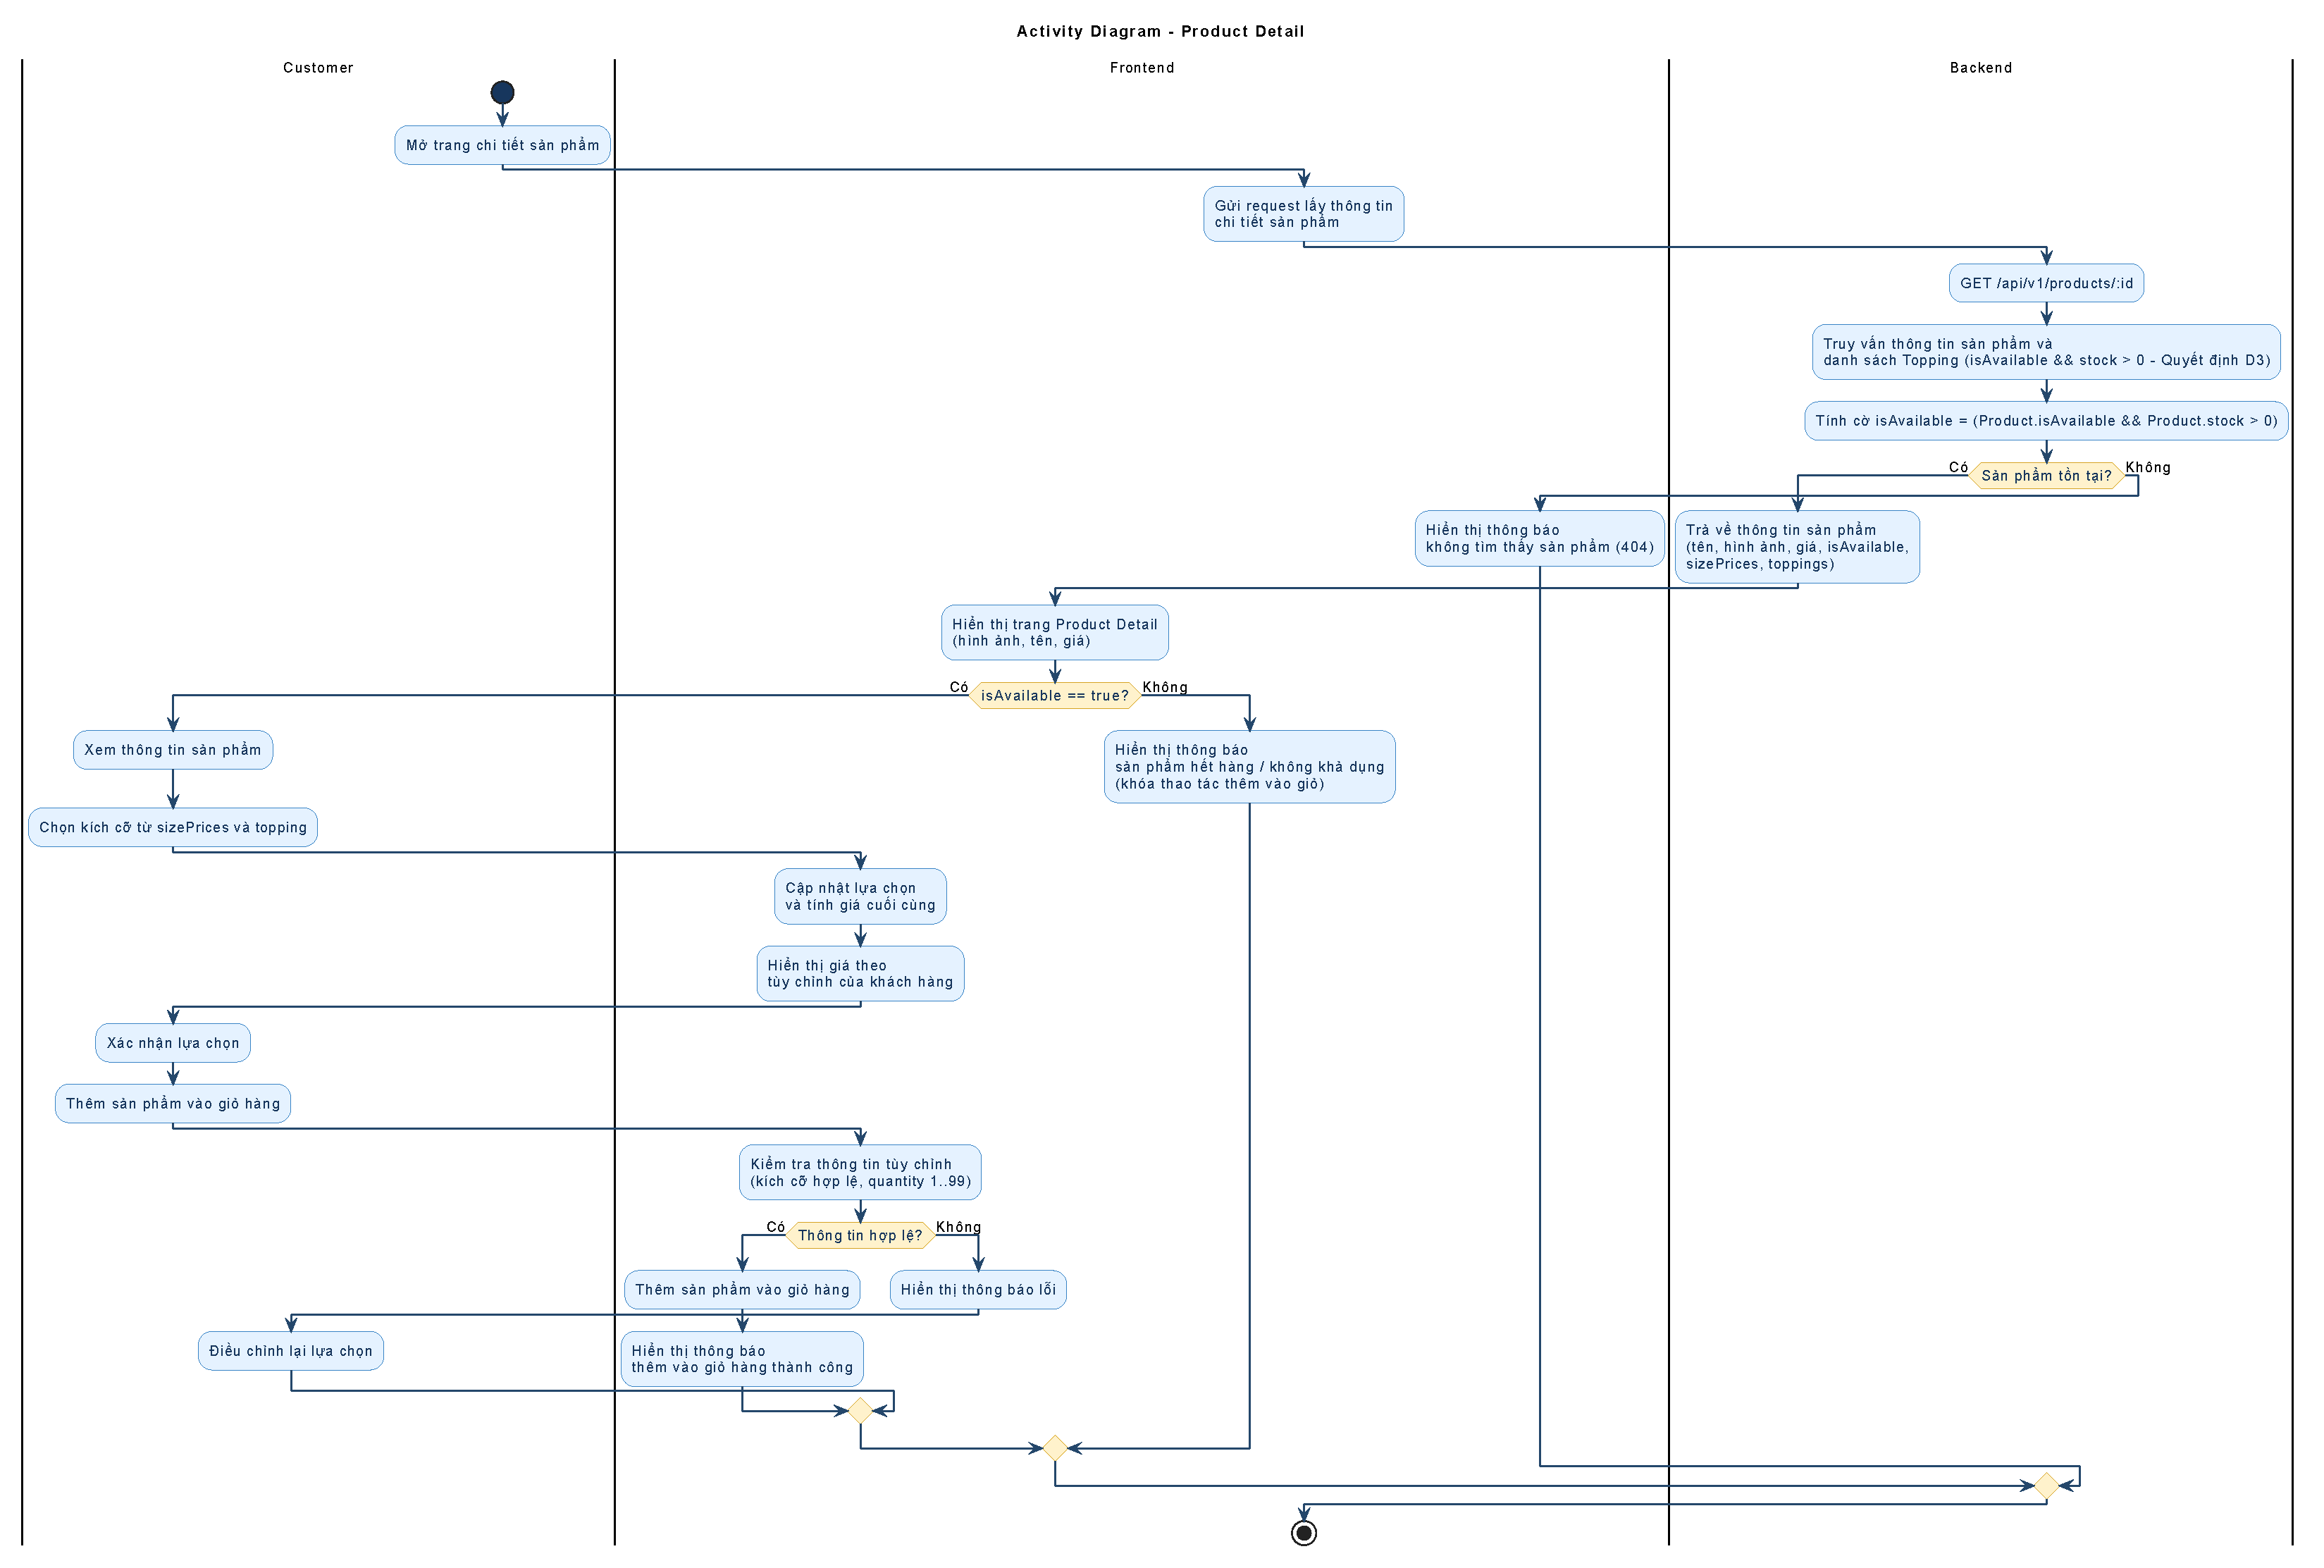
\includegraphics[width=\textwidth, height=0.80\textheight, keepaspectratio]{figures/activity-product-detail.pdf}
    \caption{Sơ đồ Hoạt động - Phân hệ Chi tiết Sản phẩm}
    \label{fig:activity-product-detail}
\end{figure}

\clearpage
\subsection{Sơ đồ Tuần tự (Sequence Diagram)}
Sơ đồ Tuần tự thể hiện các tương tác truy vấn dữ liệu chi tiết sản phẩm và danh mục topping tại Hình~\ref{fig:sequence-product-detail}.

\begin{figure}[H]
    \centering
    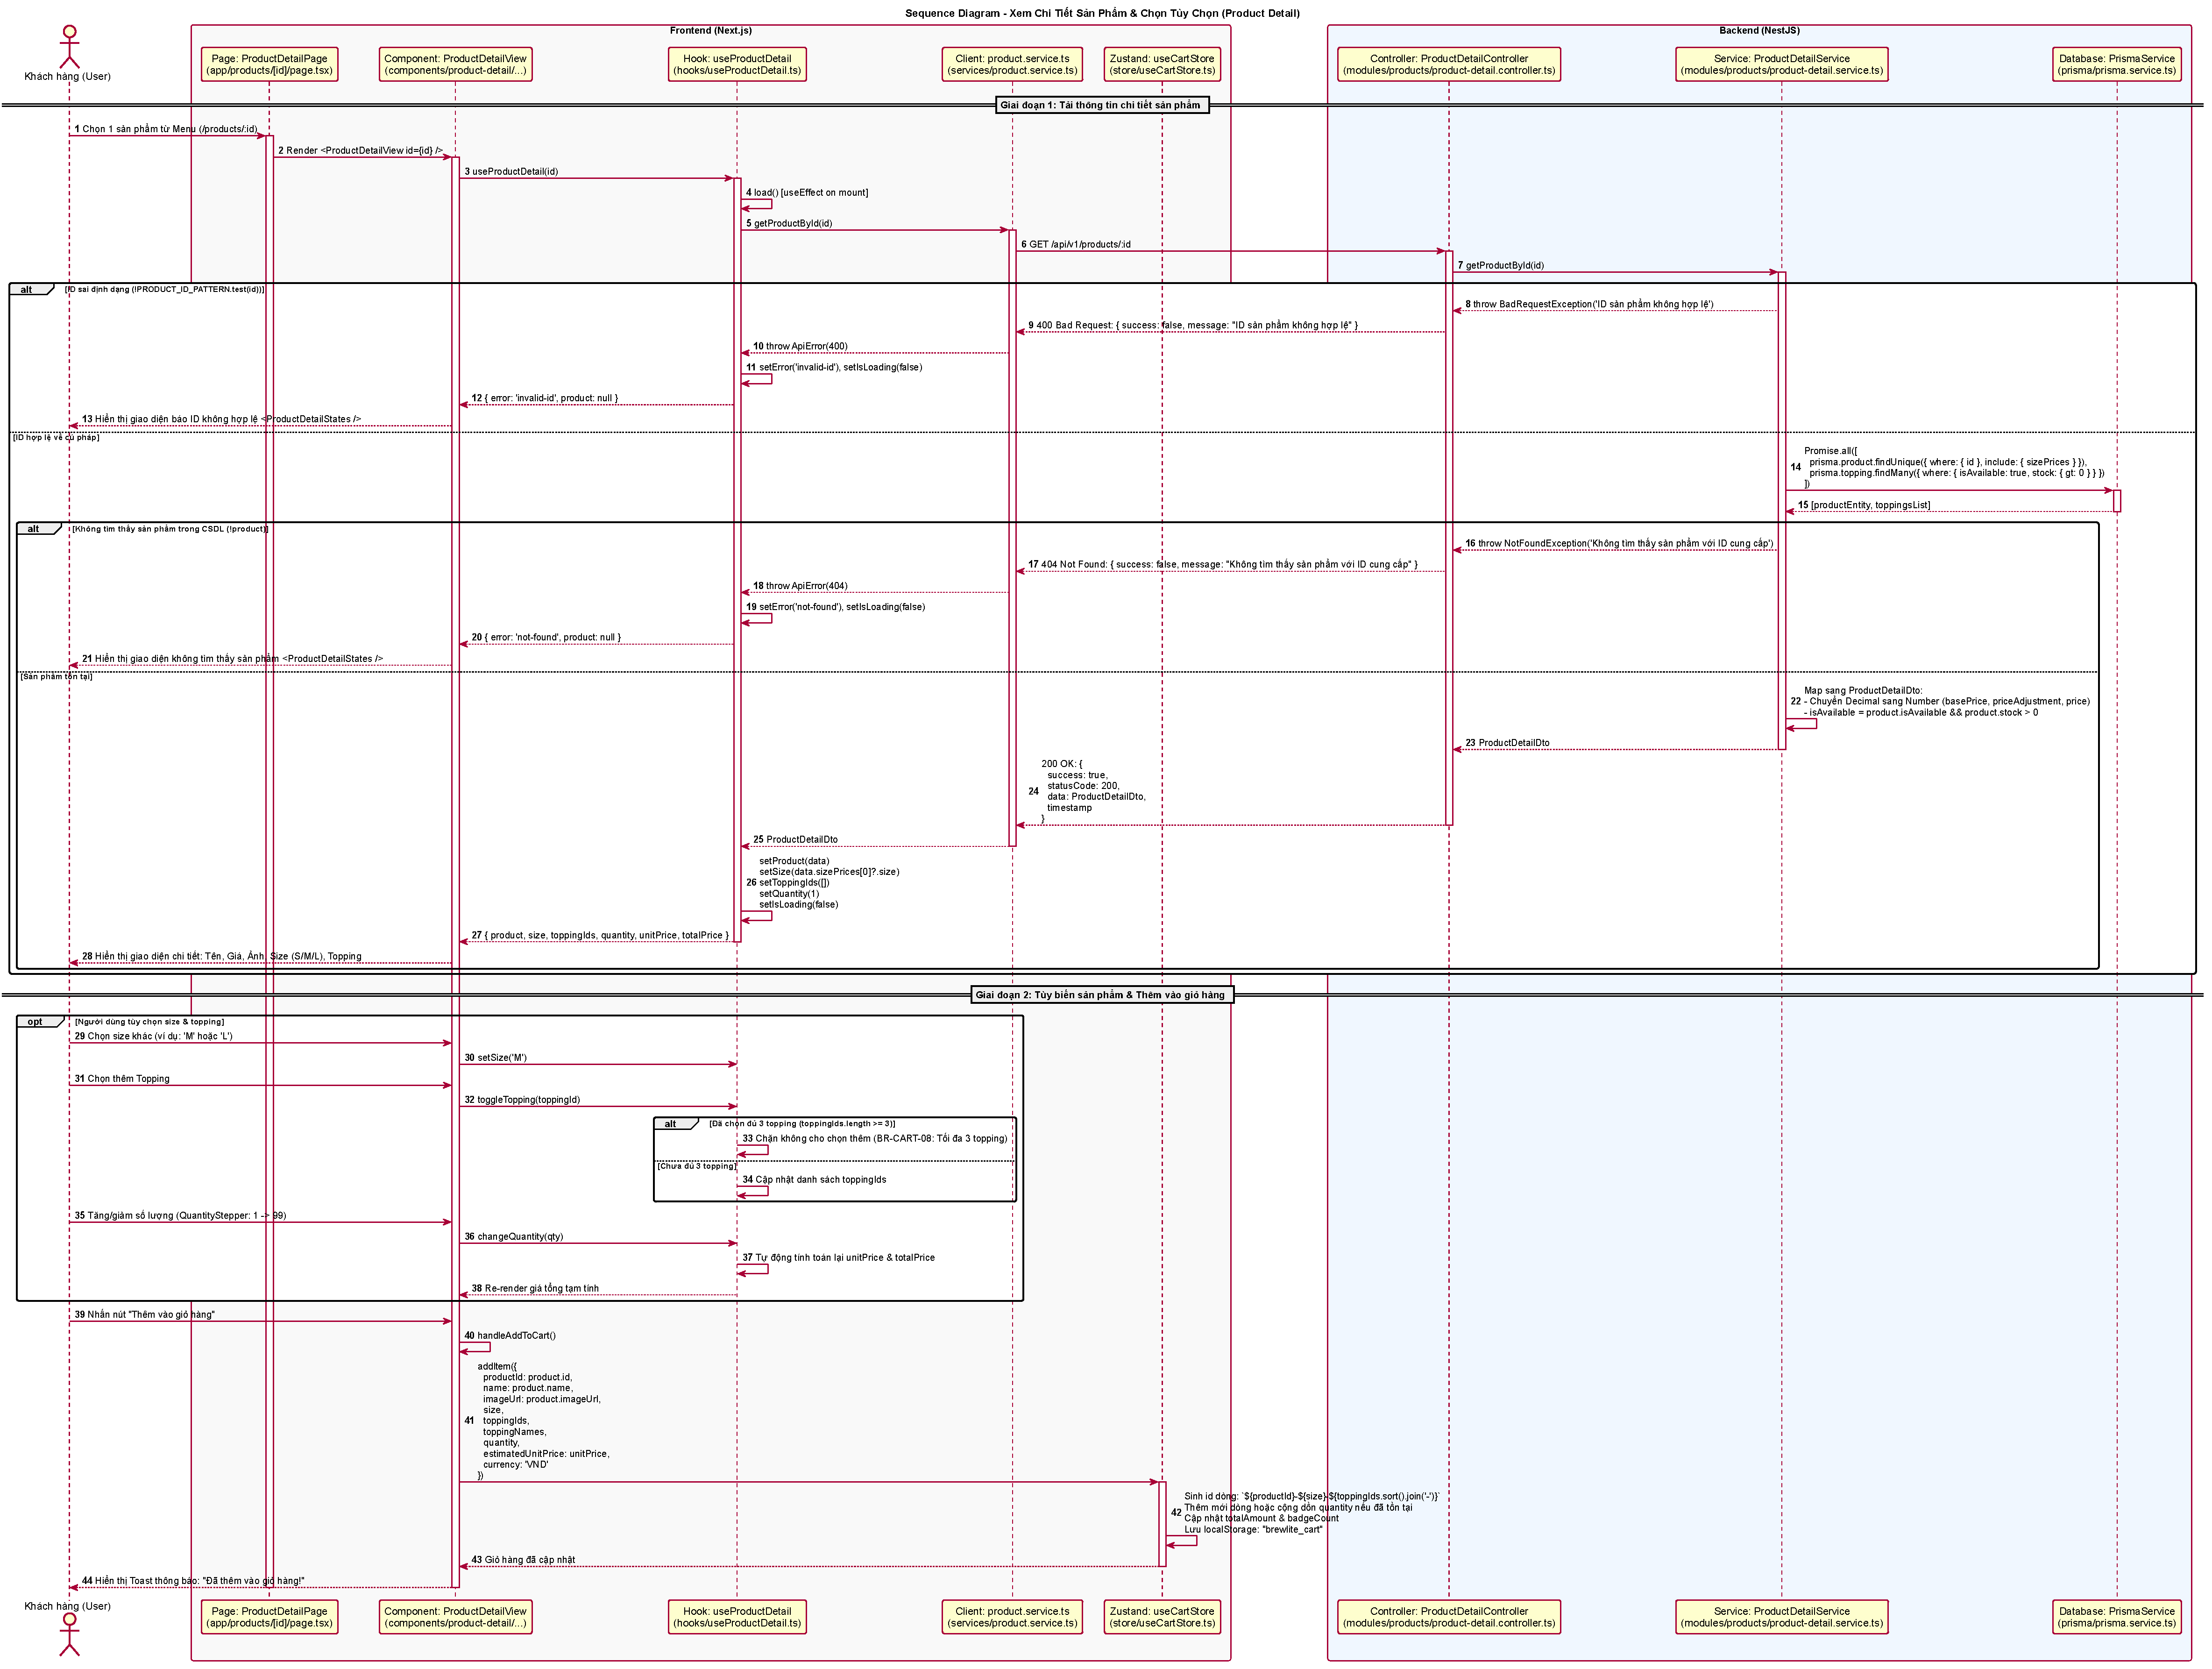
\includegraphics[width=\textwidth, height=0.80\textheight, keepaspectratio]{figures/sequence-product-detail.pdf}
    \caption{Sơ đồ Tuần tự - Phân hệ Chi tiết Sản phẩm}
    \label{fig:sequence-product-detail}
\end{figure}

\clearpage
\subsection{Hợp đồng API (API Contract)}
\begin{table}[H]
\centering
\small
\caption{Danh mục API Endpoints - Phân hệ Chi tiết Sản phẩm}
\label{tab:api-detail}
\begin{tabularx}{\textwidth}{llp{4cm}X}
\toprule
\textbf{Phương thức} & \textbf{Endpoint} & \textbf{Tham số Đường dẫn} & \textbf{Phản hồi chính} \\
\midrule
\texttt{GET} & \texttt{/api/v1/products/:id} & \texttt{id} (CUID của sản phẩm) & \texttt{200 OK}: Chi tiết sản phẩm kèm mảng \texttt{sizePrices} và thông tin \texttt{category}. Lỗi \texttt{404} nếu không tìm thấy. \\
\texttt{GET} & \texttt{/api/v1/toppings} & Không có & \texttt{200 OK}: Danh sách các loại topping đang hoạt động kèm giá và số lượng tồn. \\
\bottomrule
\end{tabularx}
\end{table}

\subsection{Ánh xạ Cơ sở dữ liệu (Database Mapping)}
\begin{itemize}
    \item Truy vấn chi tiết sản phẩm: \texttt{prisma.product.findUnique(\{ where: \{ id \}, include: \{ sizePrices: true, category: true \} \})}.
    \item Truy vấn danh sách topping: \texttt{prisma.topping.findMany(\{ where: \{ isAvailable: true \} \})}.
\end{itemize}

\subsection{Kịch bản Kiểm thử (Test Cases)}
\begin{table}[H]
\centering
\small
\caption{Tóm lược các Ca kiểm thử tiêu biểu - Phân hệ Chi tiết Sản phẩm}
\label{tab:tc-detail}
\begin{tabularx}{\textwidth}{llp{2.6cm}p{3cm}Xc}
\toprule
\textbf{Mã TC} & \textbf{Loại} & \textbf{Tiền điều kiện} & \textbf{Endpoint / Màn hình} & \textbf{Kết quả mong đợi} & \textbf{Trạng thái} \\
\midrule
\texttt{TC-DET-API-01} & Hợp lệ & ID sản phẩm tồn tại & \texttt{GET /products/:id} & HTTP 200, trả về đủ sizePrices (S, M, L) & Chưa chạy \\
\texttt{TC-DET-API-03} & Lỗi & ID không tồn tại & \texttt{GET /products/:id} & HTTP 404, message "Không tìm thấy sản phẩm" & Chưa chạy \\
\texttt{TC-DET-UI-01} & Giao diện & Mở trang chi tiết & Màn hình \texttt{/products/[id]} & Có nút "Quay lại thực đơn", nút "Thêm vào giỏ hàng" & Chưa chạy \\
\texttt{TC-DET-UI-04} & Giao diện & Chọn Size L (+10.000đ) & Tùy biến món & Đơn giá tự động cộng thêm phụ thu tương ứng & Chưa chạy \\
\bottomrule
\end{tabularx}
\end{table}

\subsection{Giao diện Người dùng}
\begin{figure}[H]
    \centering
    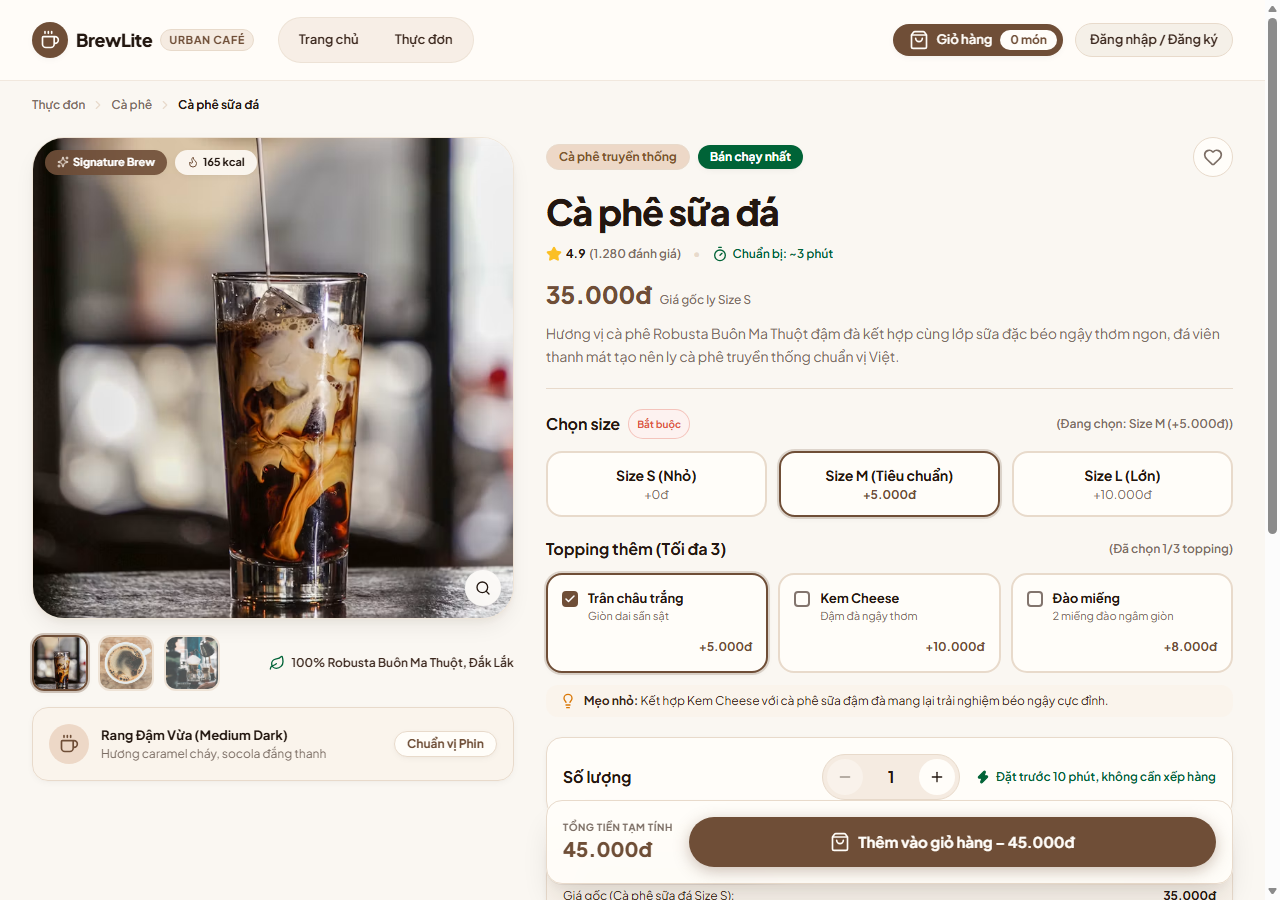
\includegraphics[width=0.92\textwidth]{figures/ui-detail.png}
    \caption{Giao diện Chi tiết món và Tùy biến Size / Topping}
    \label{fig:ui-detail}
\end{figure}

% ====== END INLINE: chapters/feature-detail ======


% ====== BEGIN INLINE: chapters/feature-cart ======
\clearpage
\section{Phân hệ Giỏ hàng (Cart)}

\subsection{Đặc tả Use Case}
Phân hệ Giỏ hàng quản lý danh sách các món đồ uống mà khách hàng đã lựa chọn kèm theo các tùy biến cụ thể trước khi tiến hành tạo đơn hàng chính thức. Để tối ưu hóa tài nguyên máy chủ và mang lại phản hồi tức thì cho người dùng, phân hệ này được thiết kế theo kiến trúc lưu trữ phía máy khách (\textit{Client-side State Management}). Sơ đồ Use Case được minh họa tại Hình~\ref{fig:usecase-cart}.

\begin{figure}[H]
    \centering
    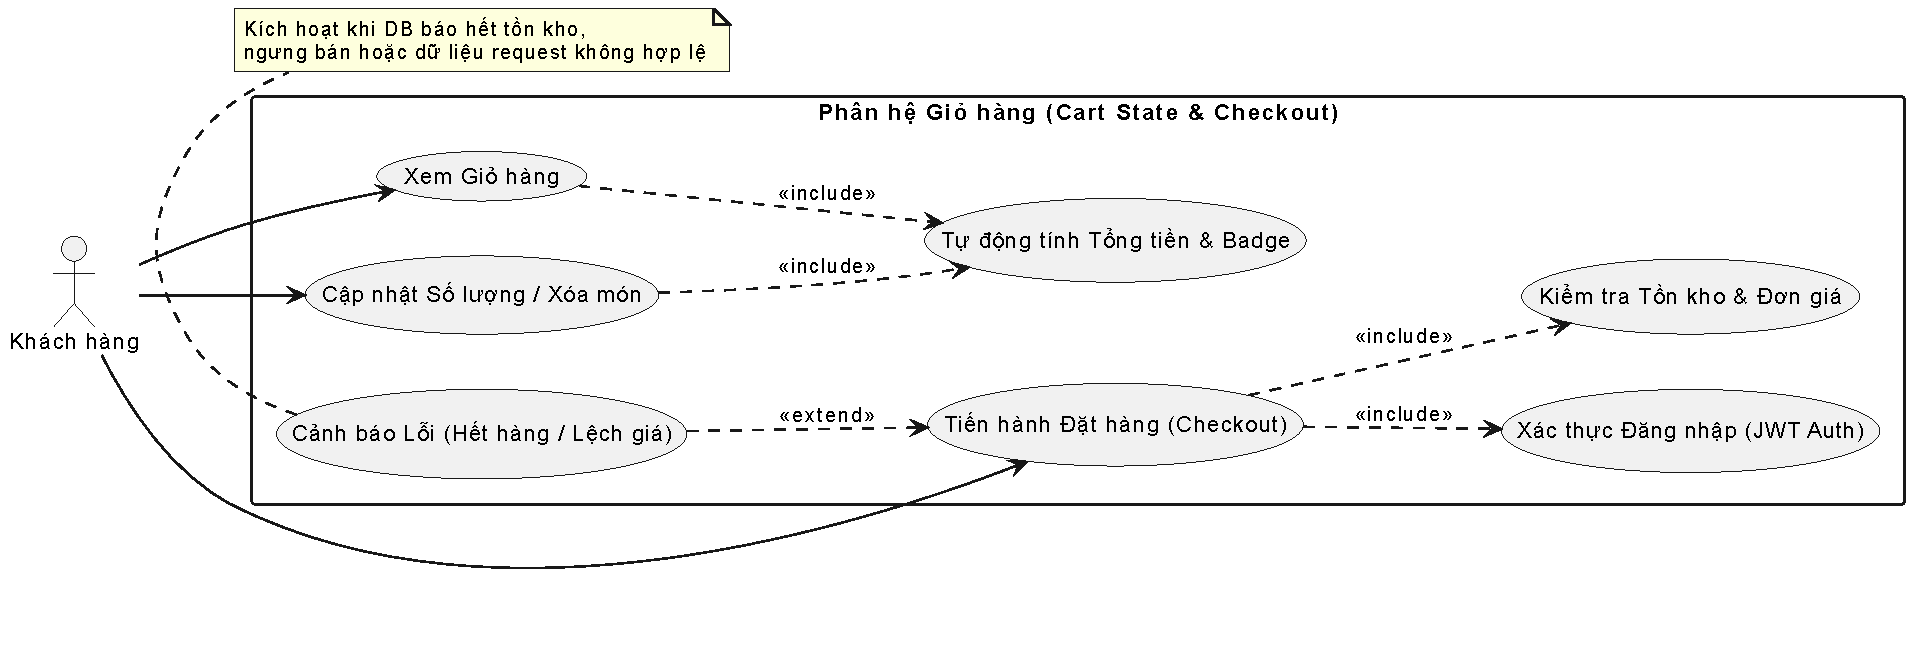
\includegraphics[width=0.75\textwidth]{figures/usecase-cart.pdf}
    \caption{Sơ đồ Use Case - Phân hệ Giỏ hàng}
    \label{fig:usecase-cart}
\end{figure}

\begin{table}[H]
\centering
\small
\caption{Đặc tả Use Case: Quản lý Giỏ hàng (UC-CART-01)}
\label{tab:uc-spec-cart}
\begin{tabularx}{\textwidth}{p{2.8cm}X}
\toprule
\textbf{Mục} & \textbf{Chi tiết Đặc tả} \\
\midrule
\textbf{Actor} & Khách vãng lai, Khách hàng đăng nhập \\
\midrule
\textbf{Tiền điều kiện} & Người dùng đã truy cập ứng dụng trên trình duyệt web. \\
\midrule
\textbf{Hậu điều kiện} & Danh sách món trong giỏ hàng, số lượng và tổng tiền tạm tính được cập nhật đồng bộ trong bộ nhớ máy khách (\texttt{localStorage} / Zustand state). \\
\midrule
\textbf{Luồng chính} & 
1. Người dùng thêm món từ trang chi tiết hoặc nhấn vào biểu tượng giỏ hàng tại thanh điều hướng (\texttt{Navbar}).\newline
2. Giao diện điều hướng sang trang \texttt{/cart}.\newline
3. Hệ thống nạp danh sách các món trong giỏ từ bộ nhớ cục bộ.\newline
4. Người dùng có thể tăng/giảm số lượng từng món, xóa từng món hoặc xóa toàn bộ giỏ.\newline
5. Bộ tính giá phía client tự động tính toán lại mục "Tạm tính" cho từng dòng và tổng giá trị đơn hàng.\newline
6. Khi người dùng nhấn "Thanh toán" (hoặc "Tiến hành đặt hàng"), hệ thống kiểm tra điều kiện đăng nhập trước khi chuyển sang bước đặt hàng. \\
\midrule
\textbf{Luồng ngoại lệ} & 
- Giỏ hàng không có sản phẩm nào: Giao diện hiển thị thông báo "Giỏ hàng của bạn đang trống" và nút điều hướng "Xem thực đơn". \\
\bottomrule
\end{tabularx}
\end{table}

\clearpage
\subsection{Sơ đồ Hoạt động (Activity Diagram)}
Quy trình quản lý thêm, sửa, xóa và tính toán giá trị giỏ hàng được thể hiện tại Hình~\ref{fig:activity-cart}.

\begin{figure}[H]
    \centering
    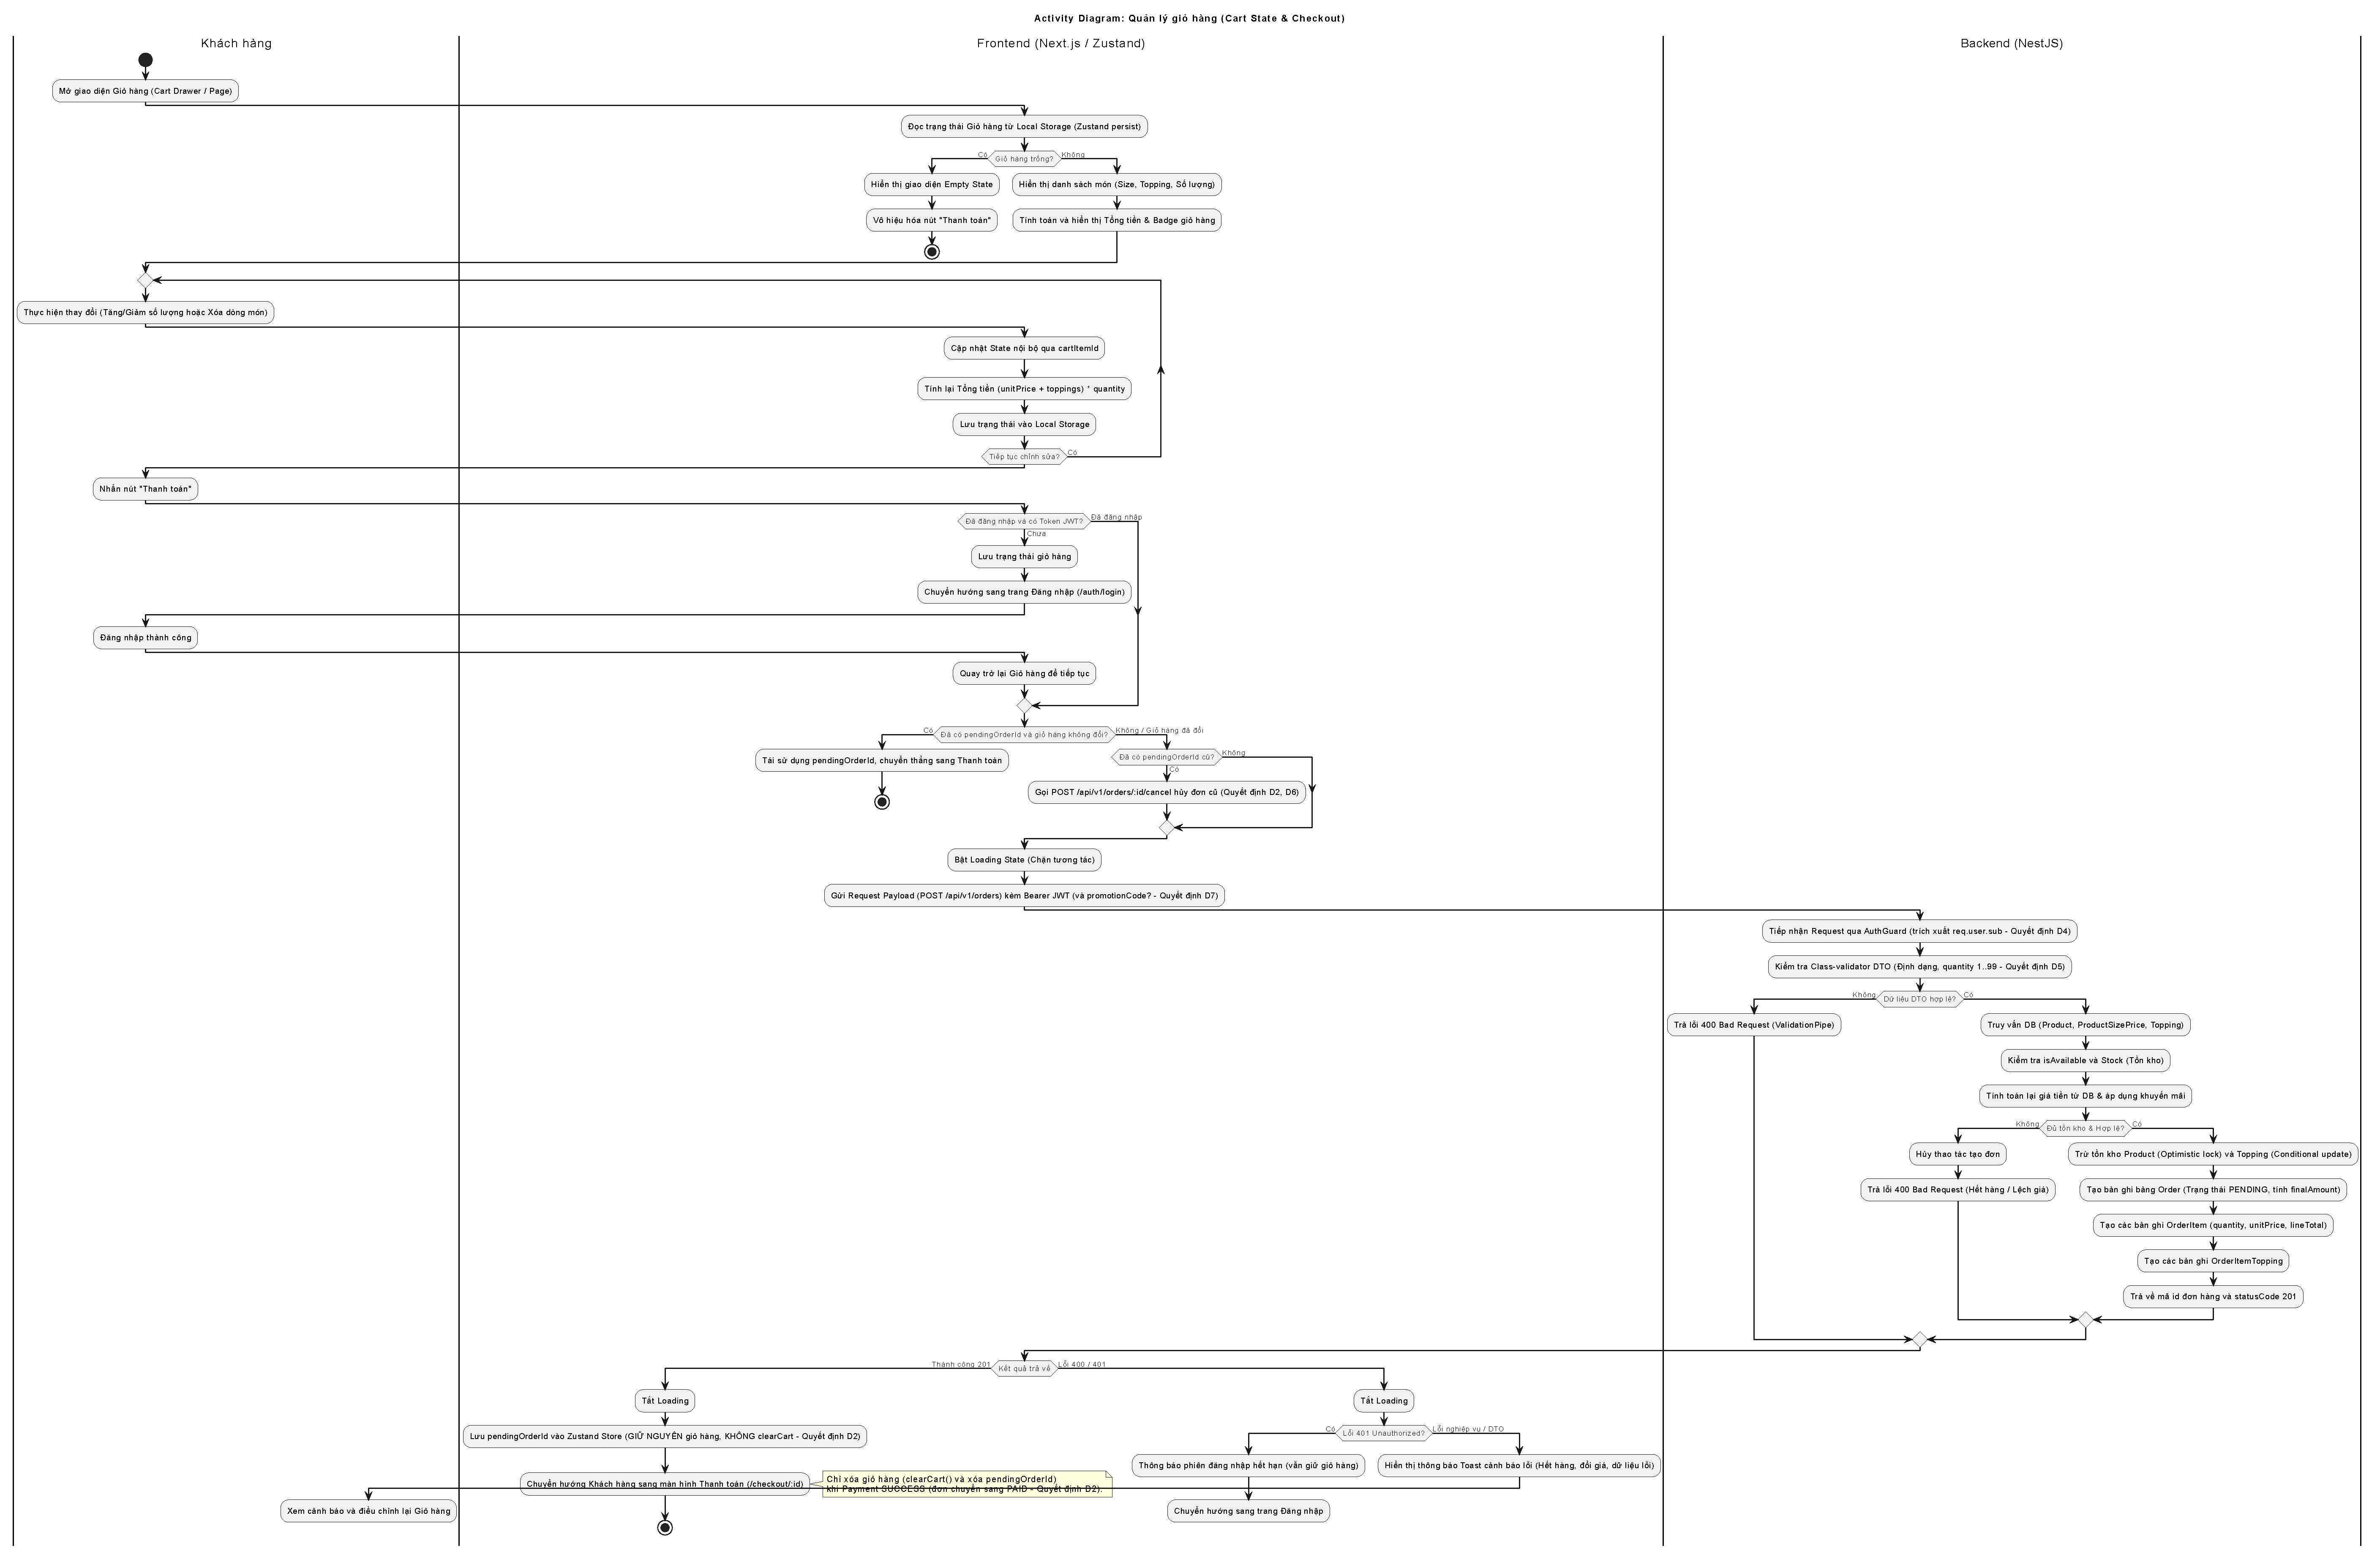
\includegraphics[width=\textwidth, height=0.80\textheight, keepaspectratio]{figures/activity-cart.pdf}
    \caption{Sơ đồ Hoạt động - Phân hệ Giỏ hàng}
    \label{fig:activity-cart}
\end{figure}

\clearpage
\subsection{Sơ đồ Tuần tự (Sequence Diagram)}
Sơ đồ Tuần tự minh họa luồng xử lý hoàn toàn khép kín ở phía Frontend giữa giao diện, Store quản lý trạng thái và LocalStorage tại Hình~\ref{fig:sequence-cart}.

\begin{figure}[H]
    \centering
    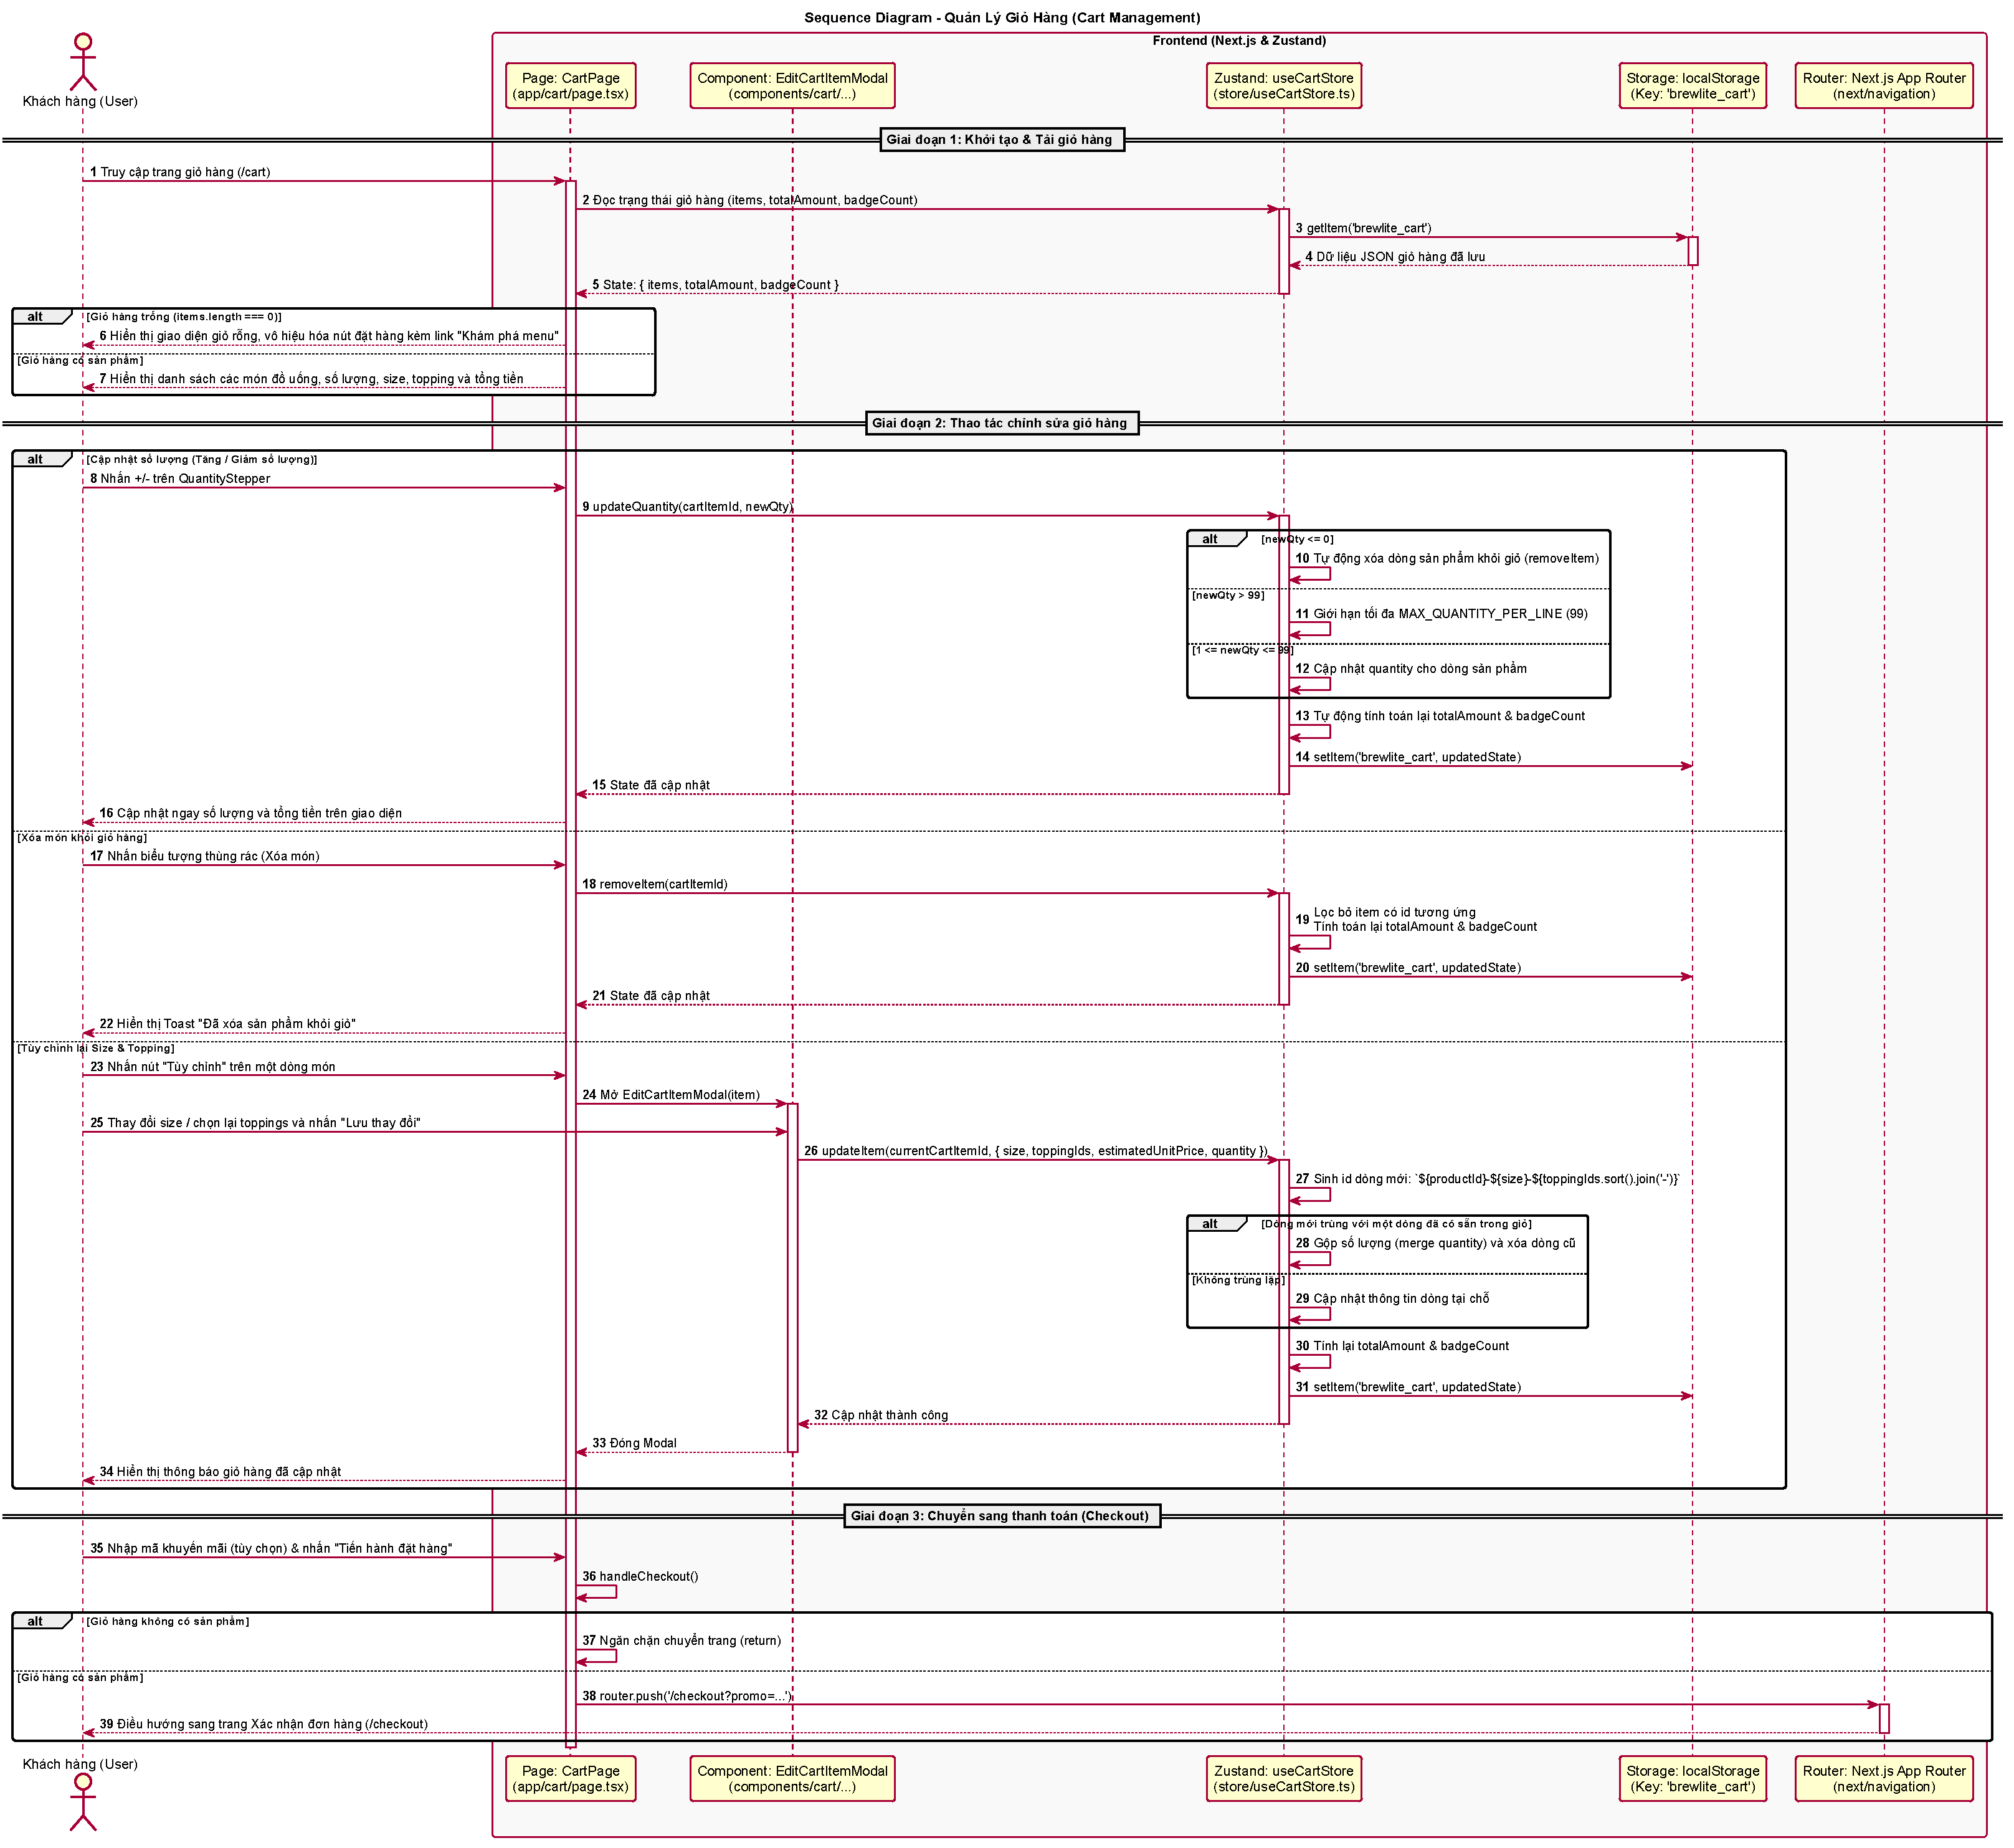
\includegraphics[width=\textwidth, height=0.80\textheight, keepaspectratio]{figures/sequence-cart.pdf}
    \caption{Sơ đồ Tuần tự - Phân hệ Giỏ hàng (Client-side Architecture)}
    \label{fig:sequence-cart}
\end{figure}

\clearpage
\subsection{Hợp đồng API và Ánh xạ Cơ sở dữ liệu}
\begin{itemize}
    \item \textbf{Đặc tính kỹ thuật (FE-Only):} Giỏ hàng trong BrewLite hoạt động hoàn toàn ở phía máy khách (\textit{Frontend-only}). Không có API endpoint riêng trên Backend và không tạo bản ghi trong cơ sở dữ liệu cho giỏ hàng tạm thời.
    \item \textbf{Cấu trúc đối tượng lưu trữ (\texttt{CartItem}):}
    Mỗi phần tử giỏ hàng được định danh bởi một khóa duy nhất sinh ra từ tổ hợp thuộc tính (\texttt{productId}, \texttt{size}, \texttt{sweetness}, \texttt{ice}, danh sách \texttt{toppings}):
    \begin{itemize}
        \item \texttt{id}: Mã duy nhất của món trong giỏ.
        \item \texttt{productId}: ID sản phẩm tham chiếu.
        \item \texttt{name}, \texttt{image}: Thông tin hiển thị.
        \item \texttt{size}, \texttt{sweetness}, \texttt{ice}: Các tùy biến đã chọn.
        \item \texttt{toppings}: Danh sách topping kèm giá đơn vị.
        \item \texttt{quantity}: Số lượng đặt (\(\ge 1\)).
        \item \texttt{unitPrice}: Đơn giá đã bao gồm phụ thu kích cỡ.
        \item \texttt{subtotal}: Tổng tiền của dòng món = \((unitPrice + \sum toppingPrice) \times quantity\).
    \end{itemize}
\end{itemize}

\subsection{Kịch bản Kiểm thử (Test Cases)}
\begin{table}[H]
\centering
\small
\caption{Tóm lược các Ca kiểm thử tiêu biểu - Phân hệ Giỏ hàng}
\label{tab:tc-cart}
\begin{tabularx}{\textwidth}{llp{2.6cm}p{3cm}Xc}
\toprule
\textbf{Mã TC} & \textbf{Loại} & \textbf{Tiền điều kiện} & \textbf{Endpoint / Màn hình} & \textbf{Kết quả mong đợi} & \textbf{Trạng thái} \\
\midrule
\texttt{TC-CART-UI-01} & Giao diện & Giỏ chưa có món & Màn hình \texttt{/cart} & Hiển thị thông báo giỏ hàng trống & Chưa chạy \\
\texttt{TC-CART-UI-02} & Nghiệp vụ & Đã thêm 1 món & Màn hình \texttt{/cart} & Hiển thị đúng tên, size, mức đường, đá, topping & Chưa chạy \\
\texttt{TC-CART-UI-03} & Nghiệp vụ & Đang có món & Nút tăng/giảm & Cập nhật số lượng và tự động tính lại tổng tiền & Chưa chạy \\
\texttt{TC-CART-UI-04} & Nghiệp vụ & Đang có món & Nút xóa món & Món bị loại bỏ khỏi danh sách, tính lại tiền & Chưa chạy \\
\bottomrule
\end{tabularx}
\end{table}

\subsection{Giao diện Người dùng}
\begin{figure}[H]
    \centering
    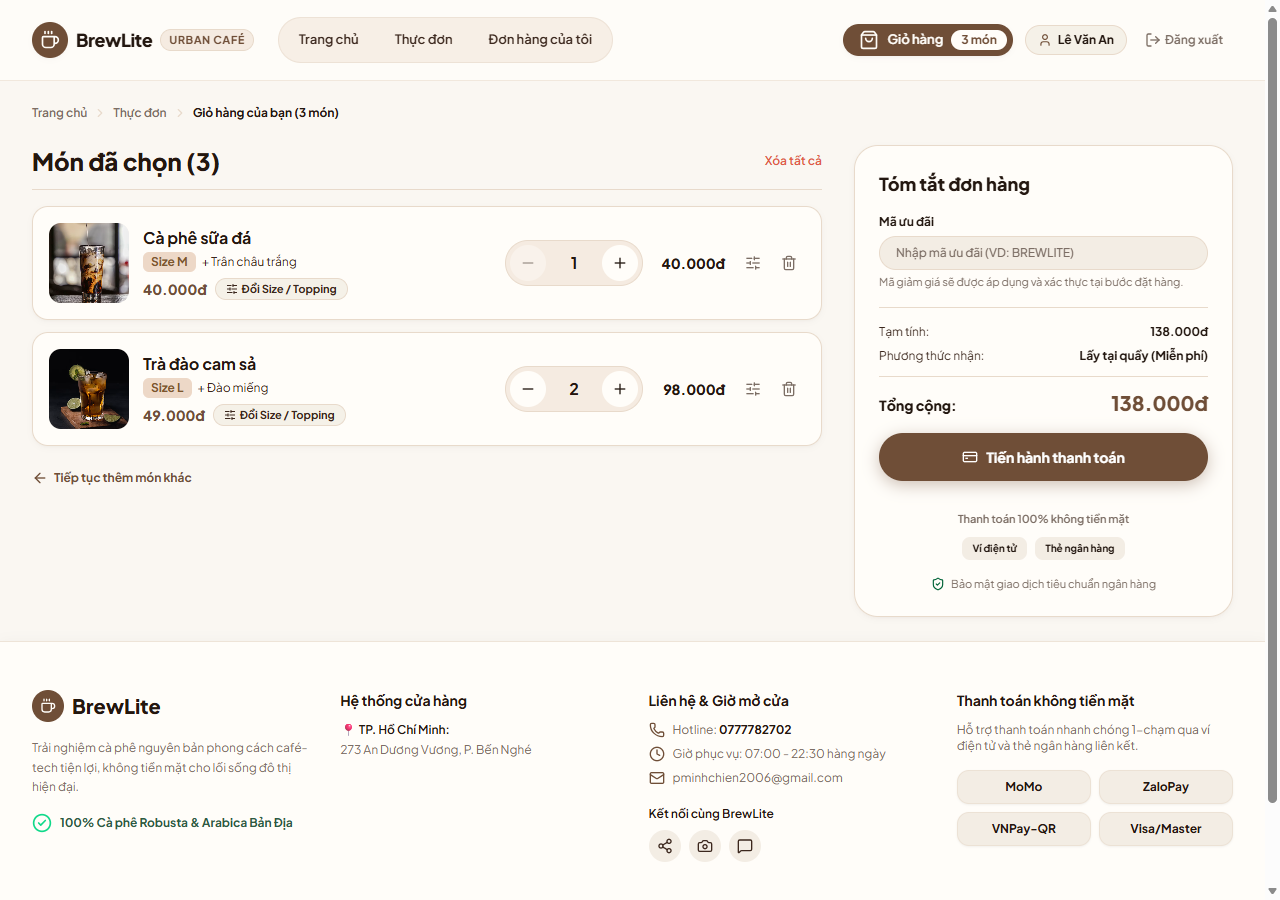
\includegraphics[width=0.92\textwidth]{figures/ui-cart.png}
    \caption{Giao diện Quản lý Giỏ hàng và Điều chỉnh số lượng BrewLite}
    \label{fig:ui-cart}
\end{figure}

% ====== END INLINE: chapters/feature-cart ======


% ====== BEGIN INLINE: chapters/feature-order ======
\clearpage
\section{Phân hệ Đặt hàng (Order)}

\subsection{Đặc tả Use Case}
Phân hệ Đặt hàng là hạt nhân nghiệp vụ của hệ thống BrewLite, chịu trách nhiệm chuyển hóa các sản phẩm trong giỏ hàng thành đơn hàng chính thức. Phân hệ tích hợp các dịch vụ tính giá (\texttt{PricingService}), kiểm tra và áp dụng khuyến mãi (\texttt{PromotionsService}), tích lũy điểm thành viên (\texttt{LoyaltyService}) và kiểm soát kho bằng khóa lạc quan (\texttt{Optimistic Locking}). Sơ đồ Use Case được minh họa tại Hình~\ref{fig:usecase-order}.

\begin{figure}[H]
    \centering
    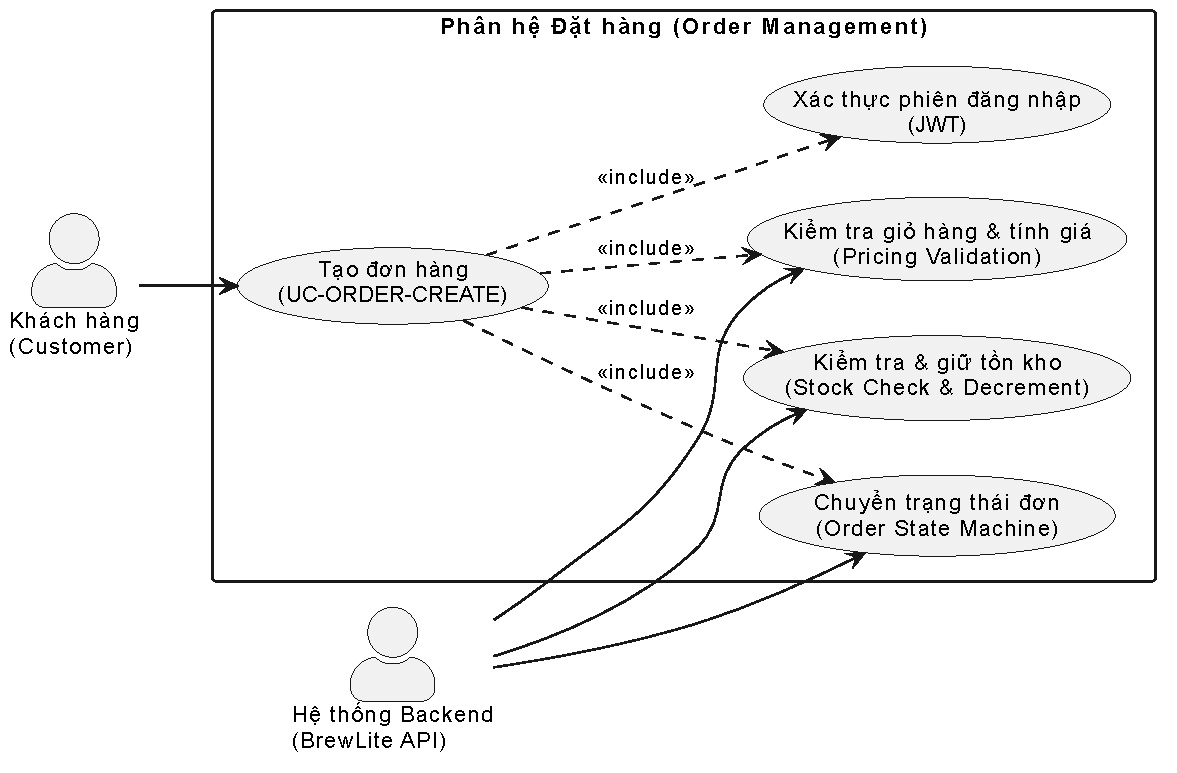
\includegraphics[width=0.75\textwidth]{figures/usecase-order.pdf}
    \caption{Sơ đồ Use Case - Phân hệ Đặt hàng}
    \label{fig:usecase-order}
\end{figure}

\begin{table}[H]
\centering
\small
\caption{Đặc tả Use Case: Tạo đơn hàng trực tuyến (UC-ORD-01)}
\label{tab:uc-spec-order}
\begin{tabularx}{\textwidth}{p{2.8cm}X}
\toprule
\textbf{Mục} & \textbf{Chi tiết Đặc tả} \\
\midrule
\textbf{Actor} & Khách hàng đã đăng nhập (Registered Customer) \\
\midrule
\textbf{Tiền điều kiện} & Khách hàng đã đăng nhập (mang Bearer JWT Token); giỏ hàng có ít nhất 1 sản phẩm. \\
\midrule
\textbf{Hậu điều kiện} & Bản ghi đơn hàng mới được tạo ở trạng thái \texttt{PENDING}; tồn kho sản phẩm được cập nhật; voucher được áp dụng; bản ghi lịch sử trạng thái được khởi tạo. \\
\midrule
\textbf{Luồng chính} & 
1. Khách hàng từ giỏ hàng nhấn "Tiến hành đặt hàng" đến trang Checkout (\texttt{/checkout}).\newline
2. Khách hàng nhập mã giảm giá (ví dụ \texttt{WELCOME10}) nếu có.\newline
3. Nhấn nút "Xác nhận đặt hàng".\newline
4. Giao diện gửi request \texttt{POST /api/v1/orders} kèm Bearer Token.\newline
5. Backend khởi động Interactive Transaction (\texttt{prisma.\$transaction}):\newline
\quad a. Kiểm tra từng sản phẩm, đối chiếu \texttt{version} và số lượng tồn kho \texttt{stock}.\newline
\quad b. Tính giá cơ bản, phụ thu size và giá topping qua \texttt{PricingService}.\newline
\quad c. Thẩm định mã giảm giá và tính số tiền giảm trừ qua \texttt{PromotionsService}.\newline
\quad d. Tính toán số điểm thưởng dự kiến tích lũy (\texttt{pointsEarned}).\newline
\quad e. Trừ tồn kho và tăng \texttt{version = version + 1} của sản phẩm.\newline
\quad f. Tạo bản ghi \texttt{orders}, các \texttt{order\_items} và \texttt{order\_item\_toppings}.\newline
\quad g. Thêm bản ghi vào \texttt{order\_status\_history} (chuyển trạng thái sang \texttt{PENDING}).\newline
6. Transaction commit thành công, trả về thông tin đơn hàng và mã số tự tăng \texttt{orderNumber} (ví dụ \#1042).\newline
7. Giao diện xóa giỏ hàng và điều hướng sang trang thanh toán (\texttt{/payment/[orderId]}). \\
\midrule
\textbf{Luồng ngoại lệ} & 
- Hết hàng hoặc tồn kho không đủ: Báo lỗi \texttt{400 Bad Request} ("Sản phẩm ... không đủ tồn kho"), rollback transaction.\newline
- Thiếu tồn kho hoặc xung đột phiên bản (Optimistic Lock Conflict): Báo lỗi \texttt{400 Bad Request} (\texttt{\"Insufficient stock or concurrent update...\"}), tự động rollback transaction.\newline
- Mã voucher không hợp lệ hoặc hết hạn: Báo lỗi \texttt{400 Bad Request} ("Mã giảm giá không hợp lệ").\newline
- Chưa đăng nhập: Báo lỗi \texttt{401 Unauthorized}, điều hướng về trang đăng nhập. \\
\bottomrule
\end{tabularx}
\end{table}

\clearpage
\subsection{Sơ đồ Hoạt động (Activity Diagram)}
Luồng hoạt động kiểm tra điều kiện tồn kho, tính giá và cam kết giao dịch tạo đơn được biểu diễn tại Hình~\ref{fig:activity-order}.

\begin{figure}[H]
    \centering
    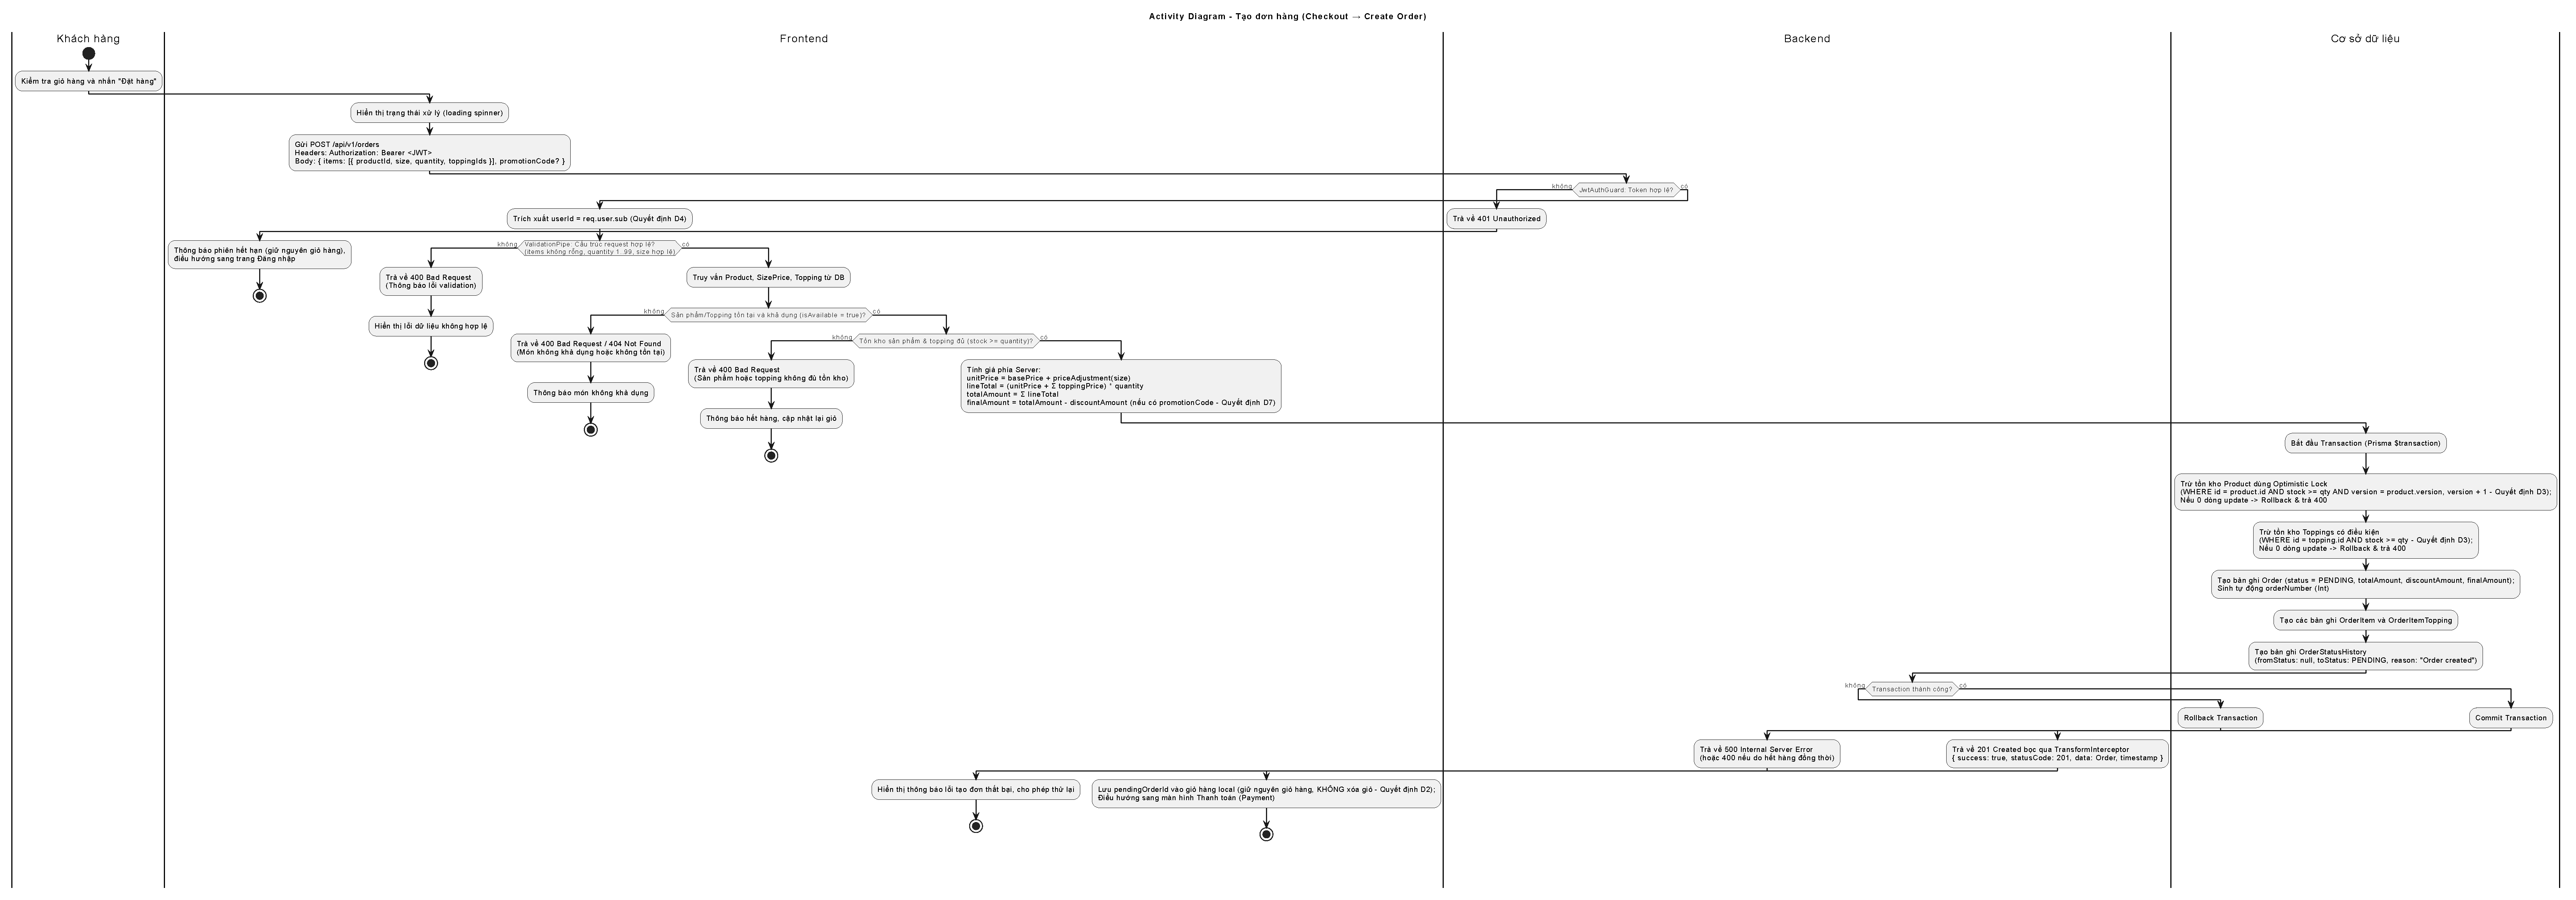
\includegraphics[width=\textwidth, height=\textheight, keepaspectratio]{figures/activity-order.pdf}
    \caption{Sơ đồ Hoạt động - Phân hệ Đặt hàng}
    \label{fig:activity-order}
\end{figure}

\clearpage
\subsection{Sơ đồ Tuần tự (Sequence Diagram)}
Sơ đồ Tuần tự minh họa chi tiết toàn bộ các lời gọi dịch vụ phối hợp trong một transaction tạo đơn hàng tại Hình~\ref{fig:sequence-order}.

\begin{figure}[H]
    \centering
    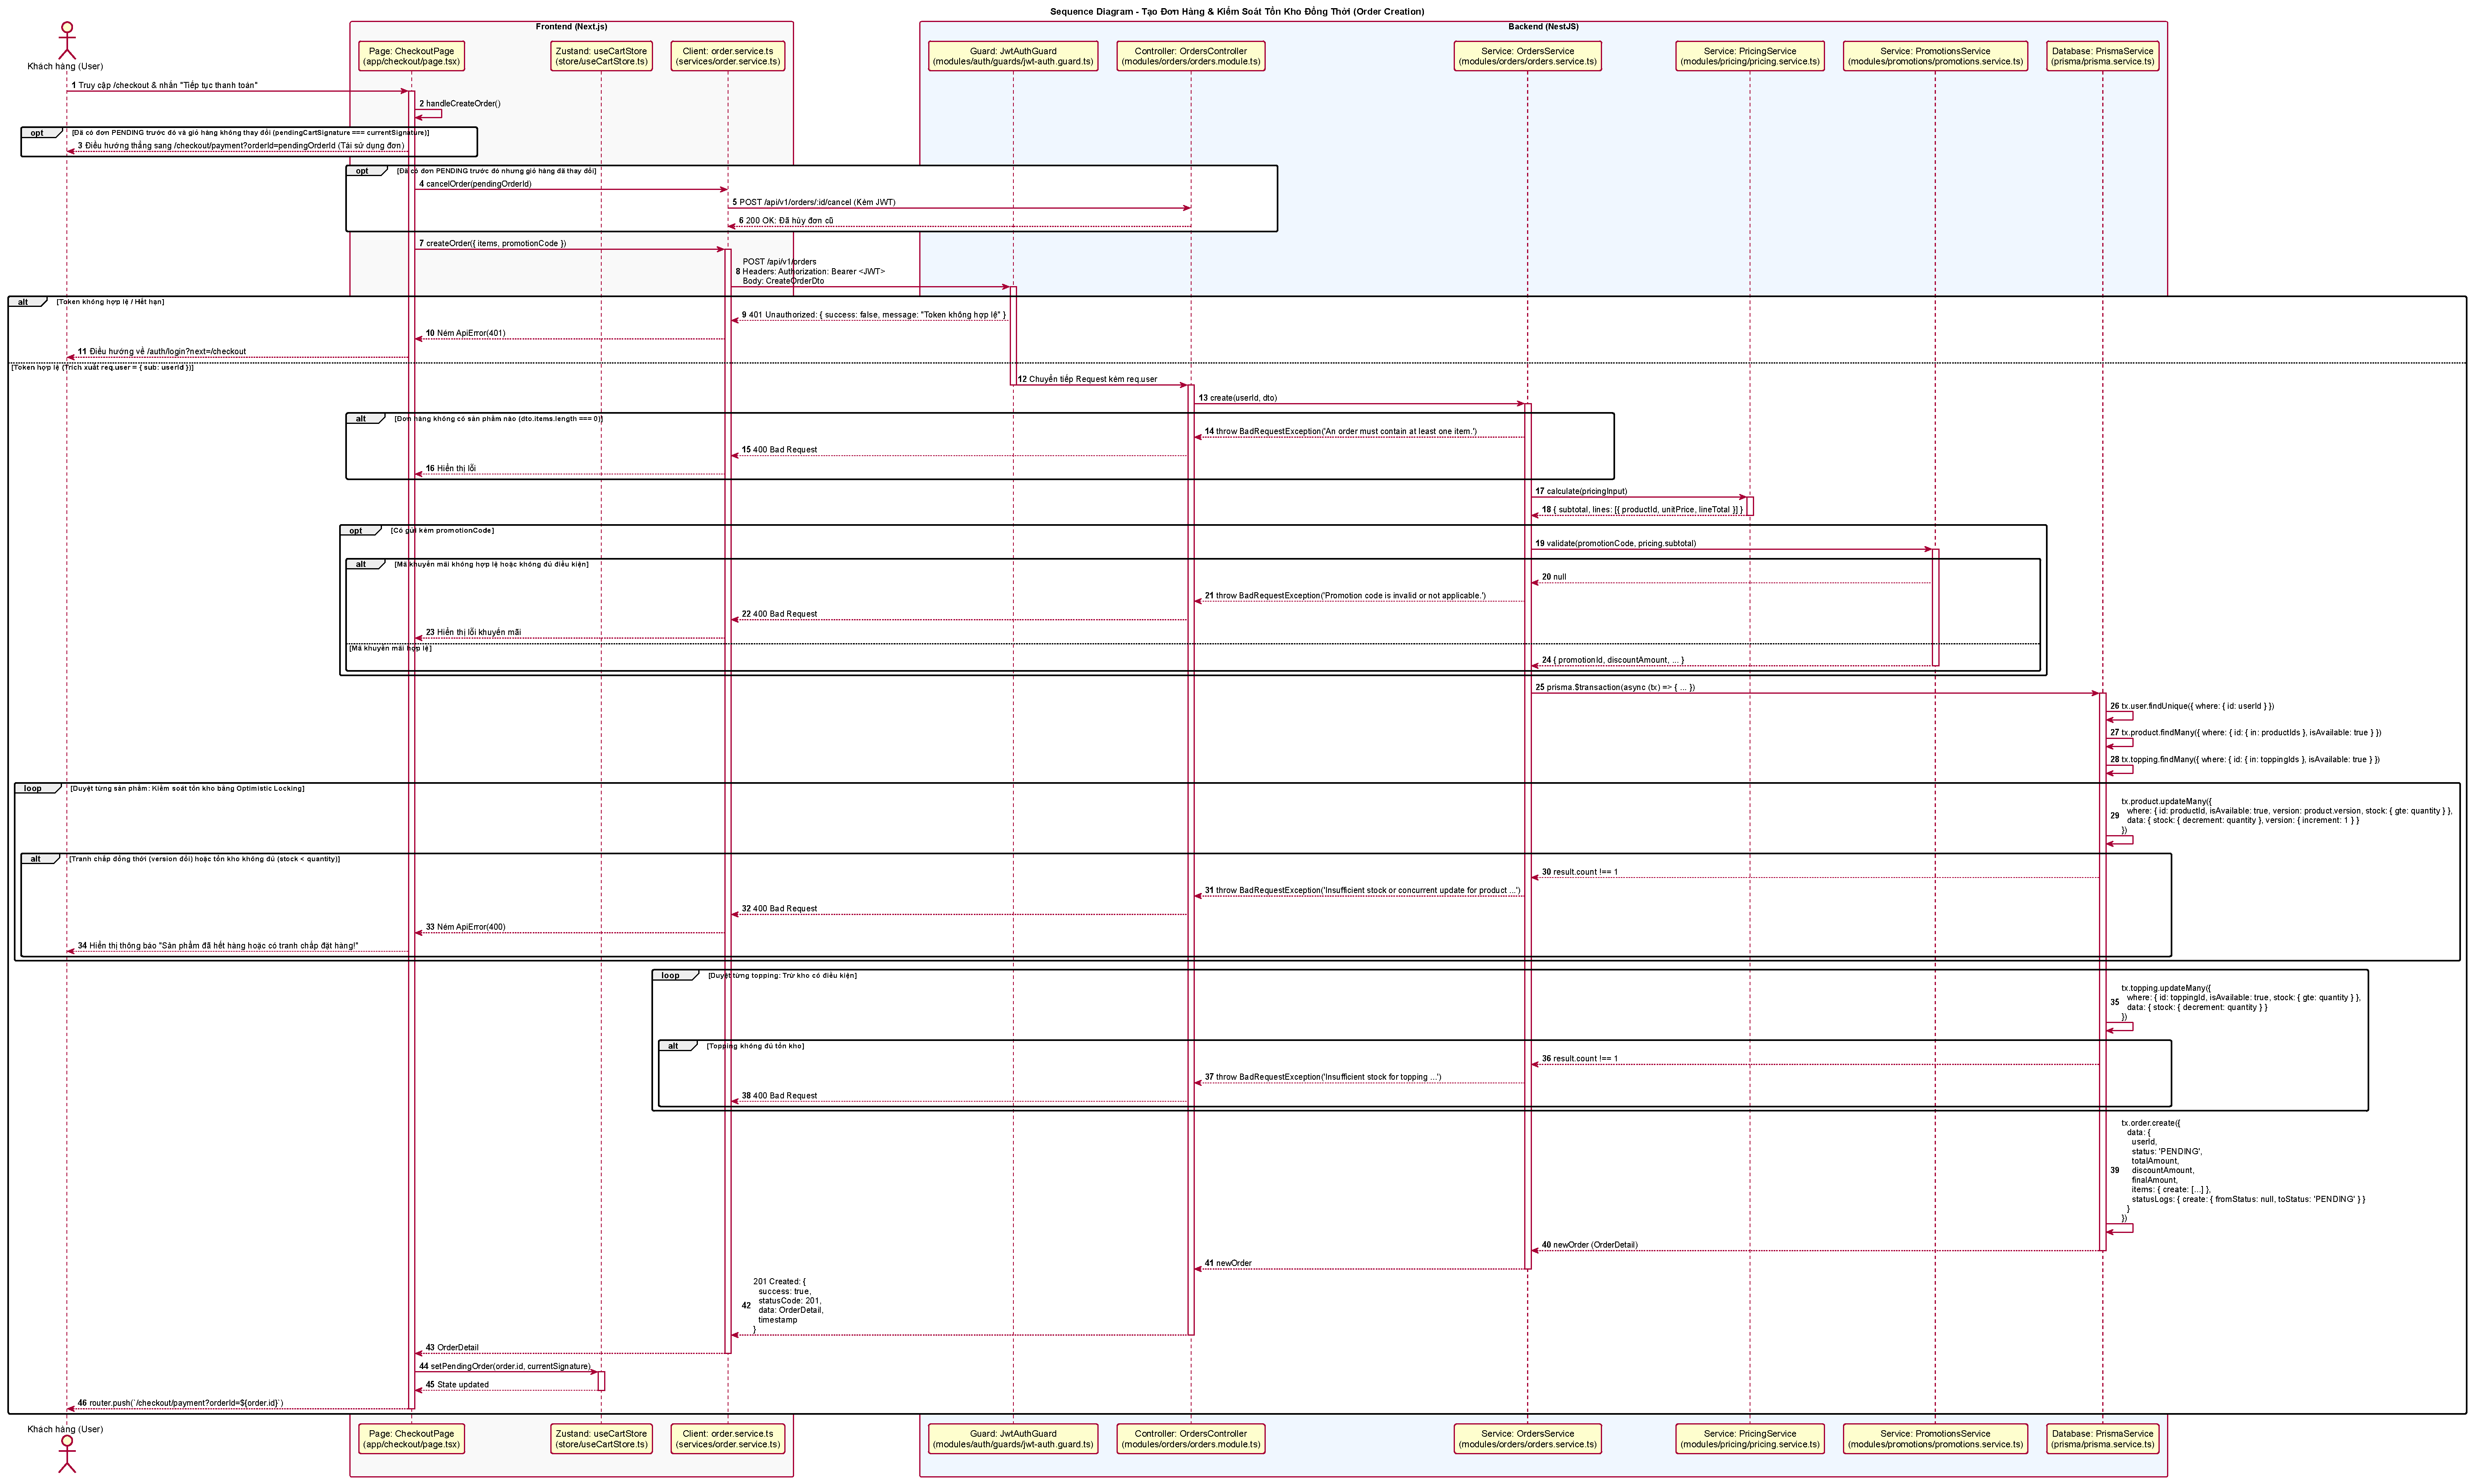
\includegraphics[width=\textwidth, height=0.80\textheight, keepaspectratio]{figures/sequence-order.pdf}
    \caption{Sơ đồ Tuần tự - Phân hệ Đặt hàng (Interactive Transaction \& Pricing Engine)}
    \label{fig:sequence-order}
\end{figure}

\clearpage
\subsection{Hợp đồng API (API Contract)}
\begin{table}[H]
\centering
\small
\caption{Danh mục API Endpoints - Phân hệ Đặt hàng}
\label{tab:api-order}
\begin{tabularx}{\textwidth}{llp{4.5cm}X}
\toprule
\textbf{Phương thức} & \textbf{Endpoint} & \textbf{Mô tả Request Payload} & \textbf{Phản hồi chính} \\
\midrule
\texttt{POST} & \texttt{/api/v1/orders} & 
\texttt{\{items: [\{productId, size, quantity, toppings\}], promotionCode?\}} (Header: \texttt{Authorization: Bearer <JWT>}) & 
\texttt{201 Created}: Trả về đơn hàng mới tạo với cấu trúc bọc chuẩn \texttt{TransformInterceptor}. Lỗi: \texttt{400 Bad Request}, \texttt{401 Unauthorized}. \\
\texttt{GET} & \texttt{/api/v1/orders/:id} & Tham số \texttt{id} của đơn hàng (Header: Bearer Token) & 
\texttt{200 OK}: Chi tiết đơn hàng, danh sách món, trạng thái xử lý và các lần thử thanh toán. \\
\bottomrule
\end{tabularx}
\end{table}

\subsection{Ánh xạ Cơ sở dữ liệu (Database Mapping)}
Quá trình tạo đơn hàng thực thi nguyên tử trong một \texttt{prisma.\$transaction}:
\begin{lstlisting}[language=SQL]
-- 1. Kiem tra va cap nhat ton kho voi Optimistic Locking
UPDATE products 
SET stock = stock - :quantity, version = version + 1
WHERE id = :productId AND version = :currentVersion AND stock >= :quantity;

-- 2. Tao ban ghi don hang chinh thuc
INSERT INTO orders (id, order_number, user_id, status, total_amount, discount_amount, final_amount, points_earned, version, created_at, updated_at)
VALUES (cuid(), nextval('orders_order_number_seq'), :userId, 'PENDING', :totalAmount, :discountAmount, :finalAmount, :pointsEarned, 0, NOW(), NOW());

-- 3. Tao cac chi tiet don hang va luu snapshot gia
INSERT INTO order_items (id, order_id, product_id, size, quantity, unit_price, line_total)
VALUES (cuid(), :orderId, :productId, :size, :quantity, :unitPrice, :lineTotal);

-- 4. Ghi nhat ky trang thai ban dau
INSERT INTO order_status_history (id, order_id, from_status, to_status, changed_by, created_at)
VALUES (cuid(), :orderId, NULL, 'PENDING', 'system', NOW());
\end{lstlisting}

\subsection{Kịch bản Kiểm thử (Test Cases)}
\begin{table}[H]
\centering
\small
\caption{Tóm lược các Ca kiểm thử tiêu biểu - Phân hệ Đặt hàng}
\label{tab:tc-order}
\begin{tabularx}{\textwidth}{llp{2.6cm}p{3cm}Xc}
\toprule
\textbf{Mã TC} & \textbf{Loại} & \textbf{Tiền điều kiện} & \textbf{Endpoint / Màn hình} & \textbf{Kết quả mong đợi} & \textbf{Trạng thái} \\
\midrule
\texttt{TC-ORD-API-01} & Hợp lệ & Đủ tồn kho, có token & \texttt{POST /orders} & HTTP 201, tạo đơn trạng thái PENDING, trừ kho & Chưa chạy \\
\texttt{TC-ORD-API-03} & Lỗi & Tồn kho không đủ & \texttt{POST /orders} & HTTP 400, rollback transaction, không trừ kho & Chưa chạy \\
\texttt{TC-ORD-API-04} & Lỗi & Xung đột version (Optimistic) & \texttt{POST /orders} & HTTP 400 Bad Request (\"Insufficient stock or concurrent update...\"), rollback & Đạt \\
\texttt{TC-ORD-API-06} & Hợp lệ & Áp voucher WELCOME10 & \texttt{POST /orders} & Giảm 10\% (tối đa 20k), finalAmount chính xác & Đạt \\
\texttt{TC-ORD-UI-01} & Giao diện & Đã đăng nhập & Trang \texttt{/checkout} & Hiển thị tóm tắt đơn, ô nhập voucher và nút đặt & Chưa chạy \\
\bottomrule
\end{tabularx}
\end{table}

\subsection{Giao diện Người dùng}
\begin{figure}[H]
    \centering
    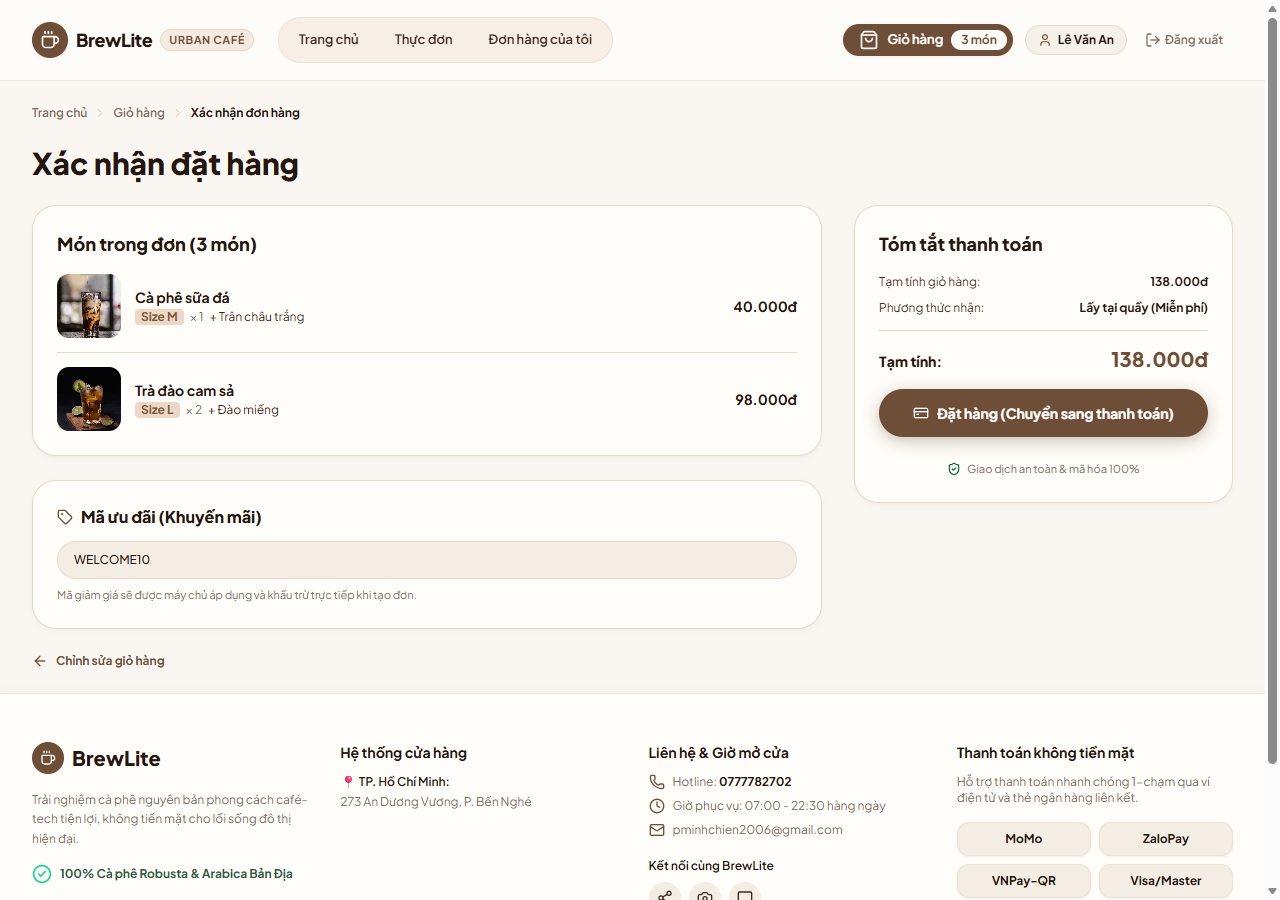
\includegraphics[width=0.92\textwidth]{figures/ui-checkout.png}
    \caption{Giao diện Xác nhận Đặt hàng và Áp dụng Khuyến mại}
    \label{fig:ui-order}
\end{figure}

% ====== END INLINE: chapters/feature-order ======


% ====== BEGIN INLINE: chapters/feature-payment ======
\clearpage
\section{Phân hệ Thanh toán (Payment)}

\subsection{Đặc tả Use Case}
Phân hệ Thanh toán chịu trách nhiệm tiếp nhận và xử lý giao dịch tài chính cho các đơn hàng đang ở trạng thái chờ. Phân hệ được thiết kế với cơ chế an toàn cấp cao: bảo vệ giao dịch bất biến (\textit{Idempotency}) để chống trùng lặp tiền khi người dùng nhấp đúp hoặc xảy ra lỗi chập chờn mạng, đồng thời hỗ trợ nhiều lượt thử lại (\textit{Retry}) cho cùng một đơn hàng thông qua quan hệ 1-N giữa \texttt{Order} và \texttt{Payment}. Sơ đồ Use Case được minh họa tại Hình~\ref{fig:usecase-payment}.

\begin{figure}[H]
    \centering
    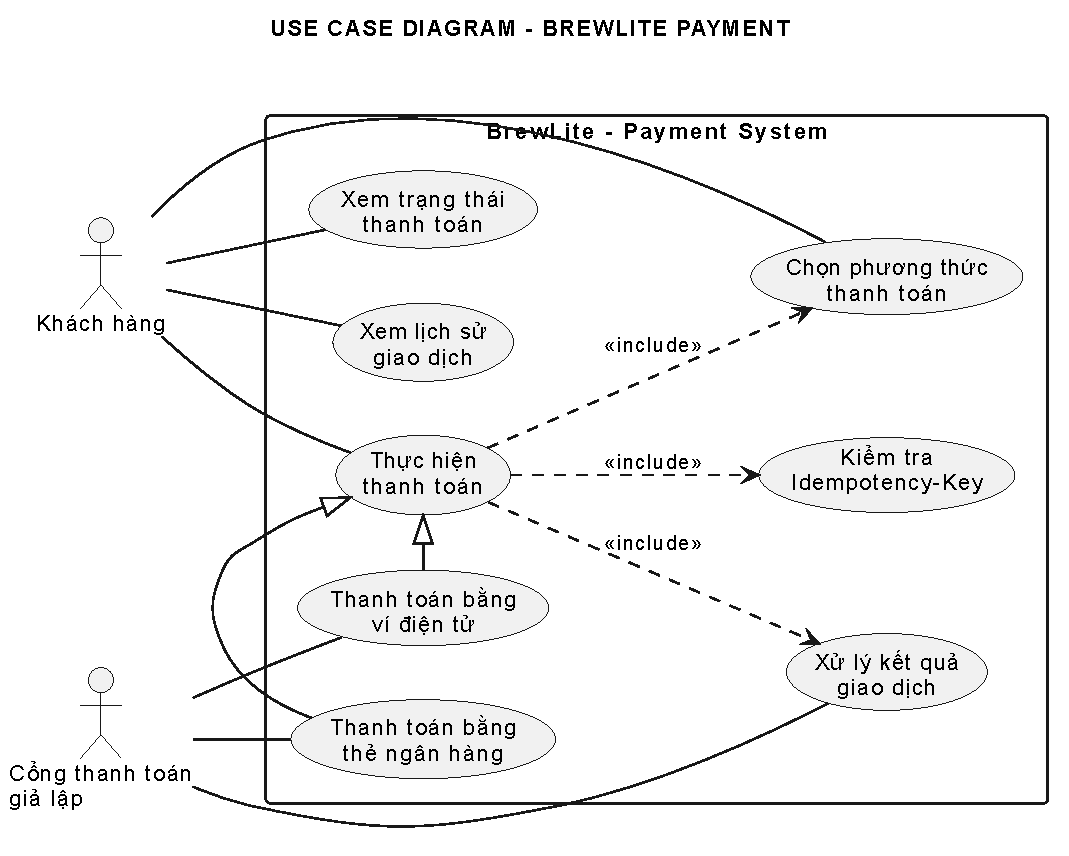
\includegraphics[width=0.75\textwidth]{figures/usecase-payment.pdf}
    \caption{Sơ đồ Use Case - Phân hệ Thanh toán}
    \label{fig:usecase-payment}
\end{figure}

\begin{table}[H]
\centering
\small
\caption{Đặc tả Use Case: Thực hiện Thanh toán Trực tuyến (UC-PAY-01)}
\label{tab:uc-spec-payment}
\begin{tabularx}{\textwidth}{p{2.8cm}X}
\toprule
\textbf{Mục} & \textbf{Chi tiết Đặc tả} \\
\midrule
\textbf{Actor} & Khách hàng đã đăng nhập, Cổng thanh toán giả lập (Mock Gateway) \\
\midrule
\textbf{Tiền điều kiện} & Đơn hàng tồn tại ở trạng thái \texttt{PENDING}; chưa được thanh toán thành công. \\
\midrule
\textbf{Hậu điều kiện} & Bản ghi thanh toán được lưu trữ; trạng thái đơn hàng chuyển thành \texttt{PAID}; điểm loyalty được cộng vào tài khoản khách hàng. \\
\midrule
\textbf{Luồng chính} & 
1. Khách hàng truy cập trang thanh toán \texttt{/payment/[orderId]}.\newline
2. Chọn phương thức thanh toán: Thẻ ngân hàng (\texttt{BANK\_CARD}) hoặc Ví điện tử (\texttt{E\_WALLET}).\newline
3. Nhấn "Thanh toán ngay".\newline
4. Trình duyệt tự động sinh mã UUID \texttt{Idempotency-Key} duy nhất và gửi request \texttt{POST /api/v1/payments}.\newline
5. PaymentsService kiểm tra \texttt{idempotencyKey}:\newline
\quad a. Nếu khóa đã tồn tại trong DB: Gọi \texttt{replayExistingPayment()} đối chiếu mã băm SHA-256 trên \texttt{\{orderId, method\}}. Nếu trùng khớp, trả lại kết quả đã lưu mà không gọi lại Mock Gateway; nếu sai lệch tải trọng, ném ngoại lệ \texttt{409 Conflict}.\newline
\quad b. Nếu là khóa mới: Khởi tạo giao dịch \texttt{payments} trong \texttt{prisma.\$transaction} với trạng thái \texttt{PENDING} và lưu mã băm \texttt{requestHash}.\newline
\quad c. Xử lý tranh chấp đồng thời: Nếu hai request cùng gửi một khóa, lỗi trùng khóa Unique (\texttt{P2002}) được bắt trong khối \texttt{catch}, tự động truy vấn lại giao dịch vừa tạo và phát lại (\textit{replay}) kết quả an toàn.\newline
6. Backend gọi Mock Payment Gateway để xác thực giao dịch.\newline
7. Khi Gateway phản hồi thành công (\texttt{SUCCESS}):\newline
\quad a. Cập nhật bản ghi \texttt{payments} thành \texttt{SUCCESS} kèm \texttt{transactionRef}.\newline
\quad b. Cập nhật đơn hàng: \texttt{status = PAID}, \texttt{paidAt = NOW()}.\newline
\quad c. Cộng điểm tích lũy mới vào \texttt{users.loyalty\_points}.\newline
\quad d. Ghi nhận giao dịch cộng điểm vào \texttt{loyalty\_transactions} (type: \texttt{EARNED}).\newline
\quad e. Ghi nhật ký vào \texttt{order\_status\_history} (PENDING \(\to\) PAID).\newline
8. Giao diện thông báo thanh toán thành công và điều hướng sang trang Lịch sử đơn hàng. \\
\midrule
\textbf{Luồng ngoại lệ} & 
- Gateway từ chối hoặc giao dịch thất bại: Cập nhật bản ghi payment thành \texttt{FAILED}, đơn hàng chuyển sang \texttt{PAYMENT\_FAILED}, cho phép khách hàng nhấn thử lại (tạo lượt payment mới).\newline
- Đơn hàng đã được thanh toán trước đó: Báo lỗi \texttt{400 Bad Request} ("Đơn hàng đã được thanh toán").\newline
- Trùng Idempotency-Key nhưng khác payload: Báo lỗi \texttt{409 Conflict} (\"Idempotency-Key đã được sử dụng với nội dung khác\"). \\
\bottomrule
\end{tabularx}
\end{table}

\clearpage
\subsection{Sơ đồ Hoạt động (Activity Diagram)}
Quy trình thẩm định Idempotency, gọi cổng thanh toán và xử lý kết quả giao dịch được mô tả tại Hình~\ref{fig:activity-payment}.

\begin{figure}[H]
    \centering
    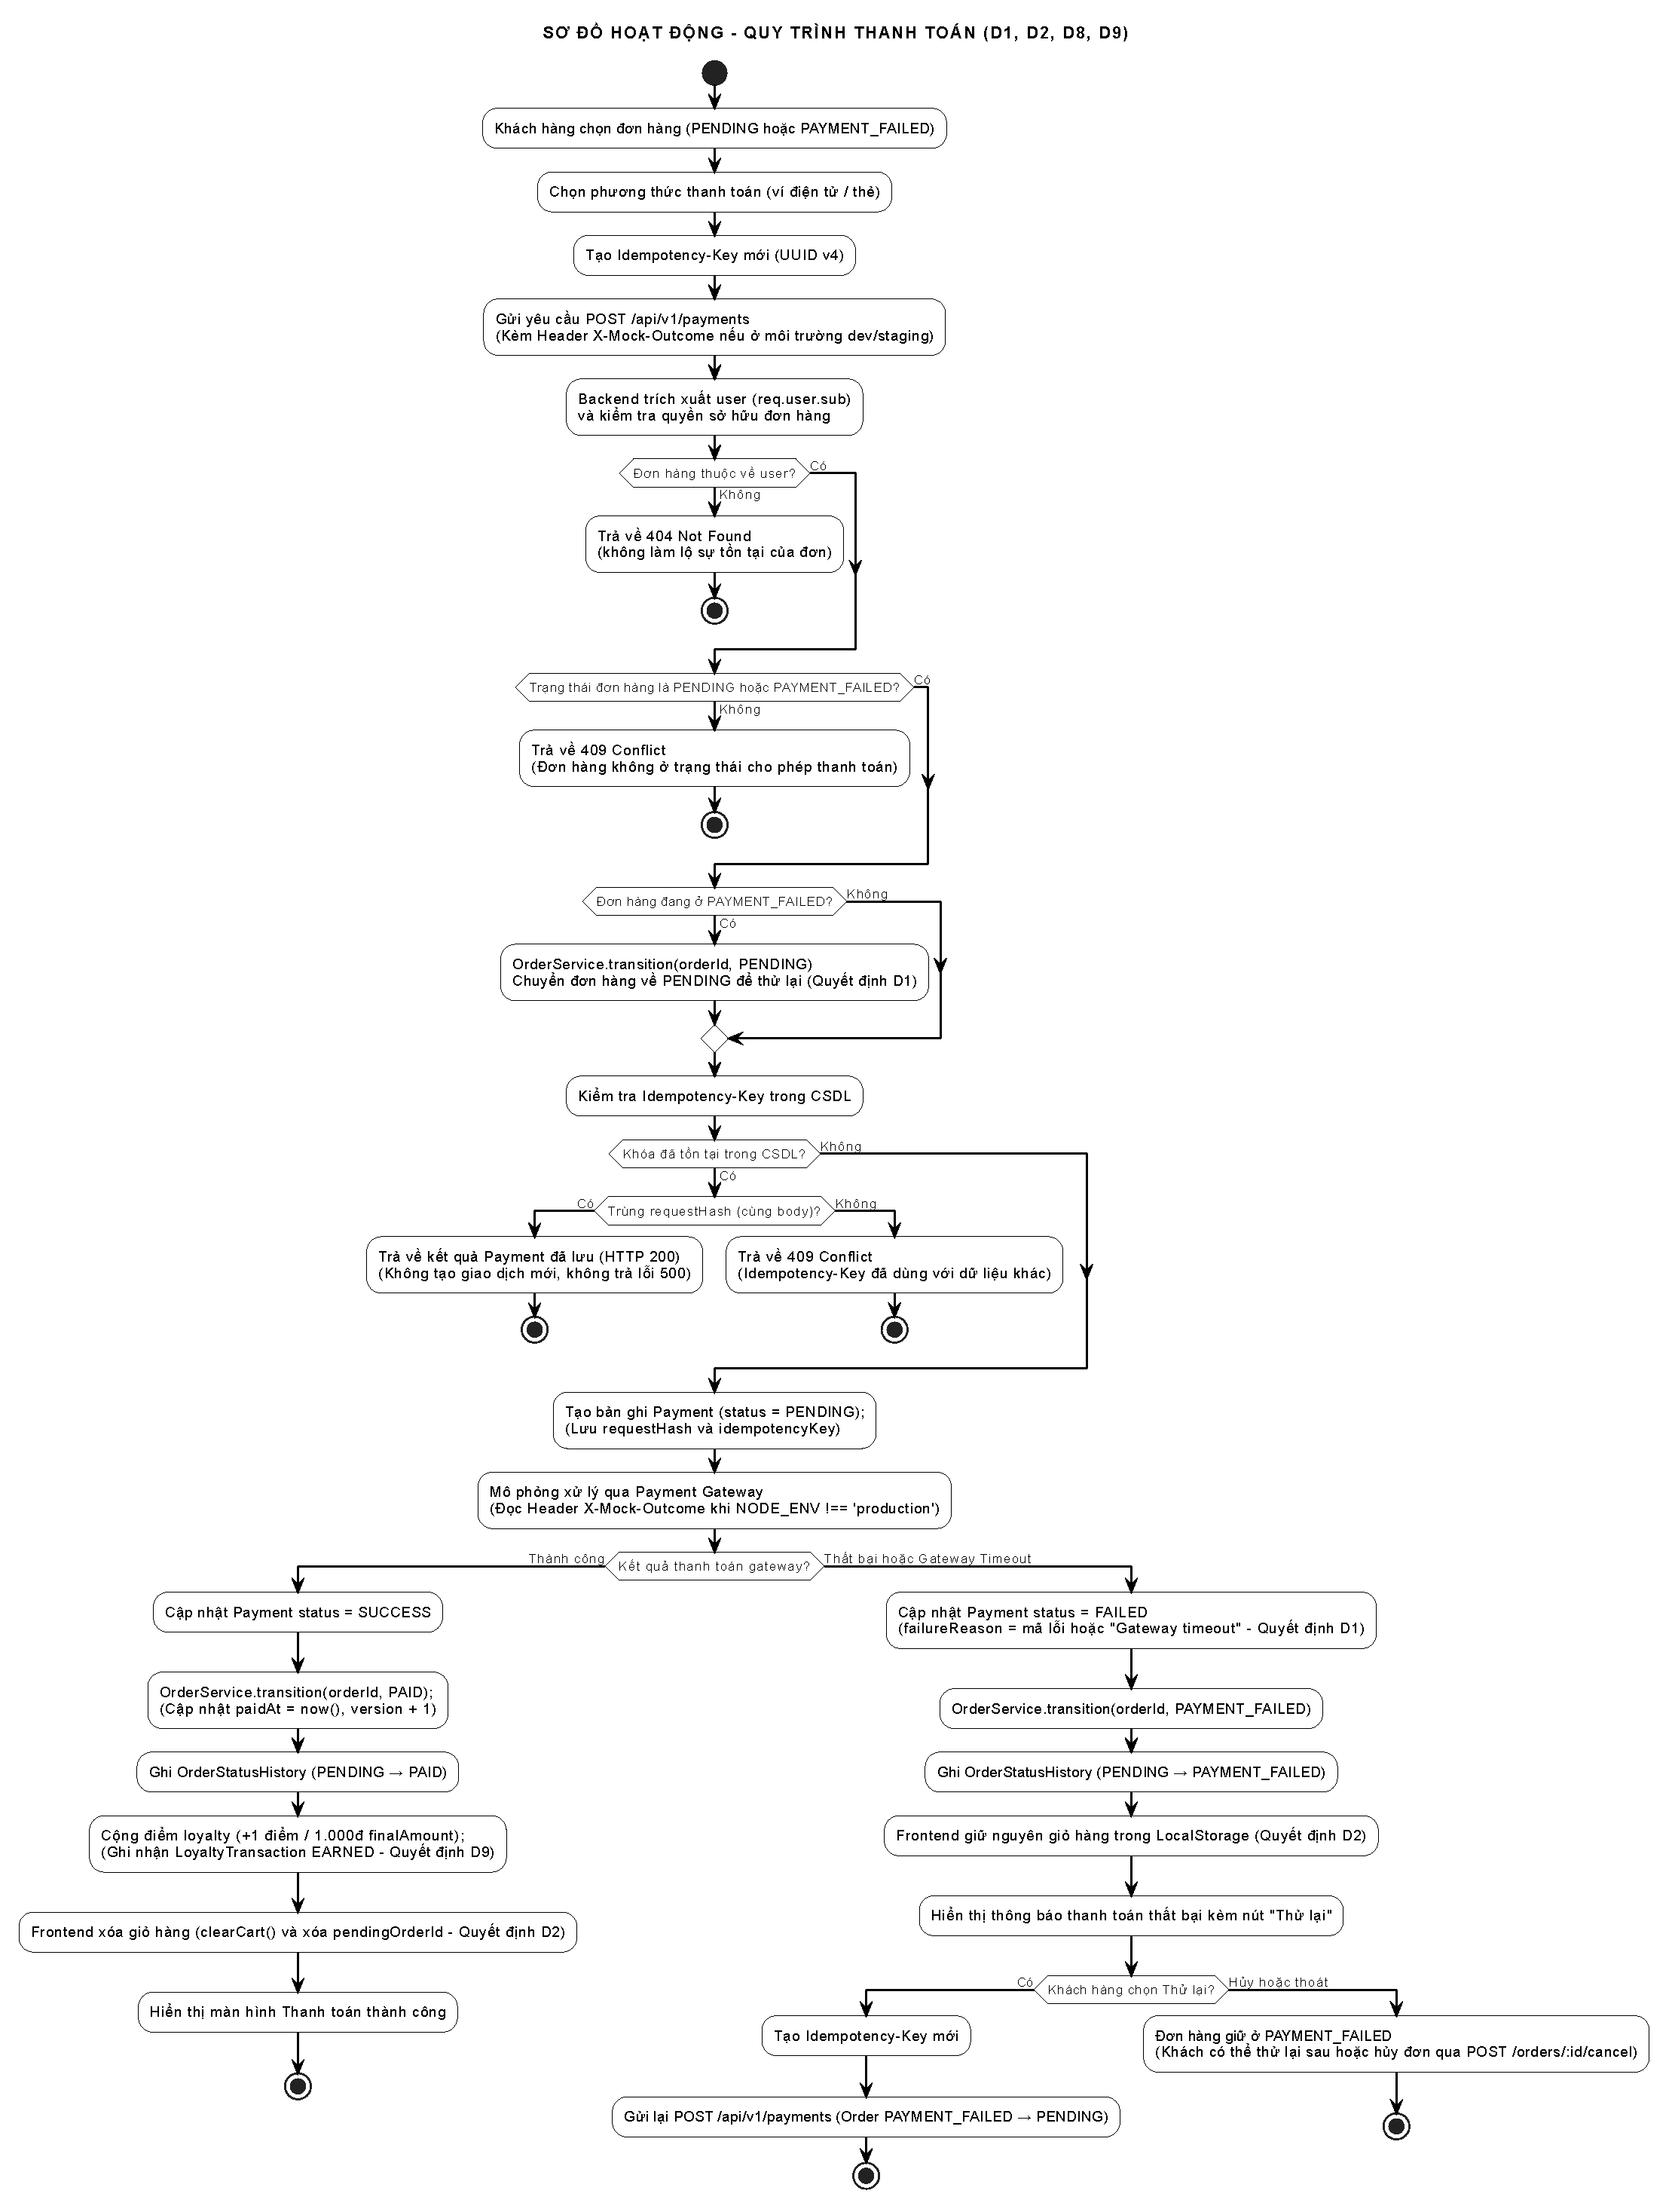
\includegraphics[width=\textwidth, height=0.80\textheight, keepaspectratio]{figures/activity-payment.pdf}
    \caption{Sơ đồ Hoạt động - Phân hệ Thanh toán}
    \label{fig:activity-payment}
\end{figure}

\clearpage
\subsection{Sơ đồ Tuần tự (Sequence Diagram)}
Sơ đồ Tuần tự phản ánh toàn diện các luồng tương tác giữa Frontend, PaymentsController, PaymentsService, Prisma DB và Mock Payment Gateway tại Hình~\ref{fig:sequence-payment}.

\begin{figure}[H]
    \centering
    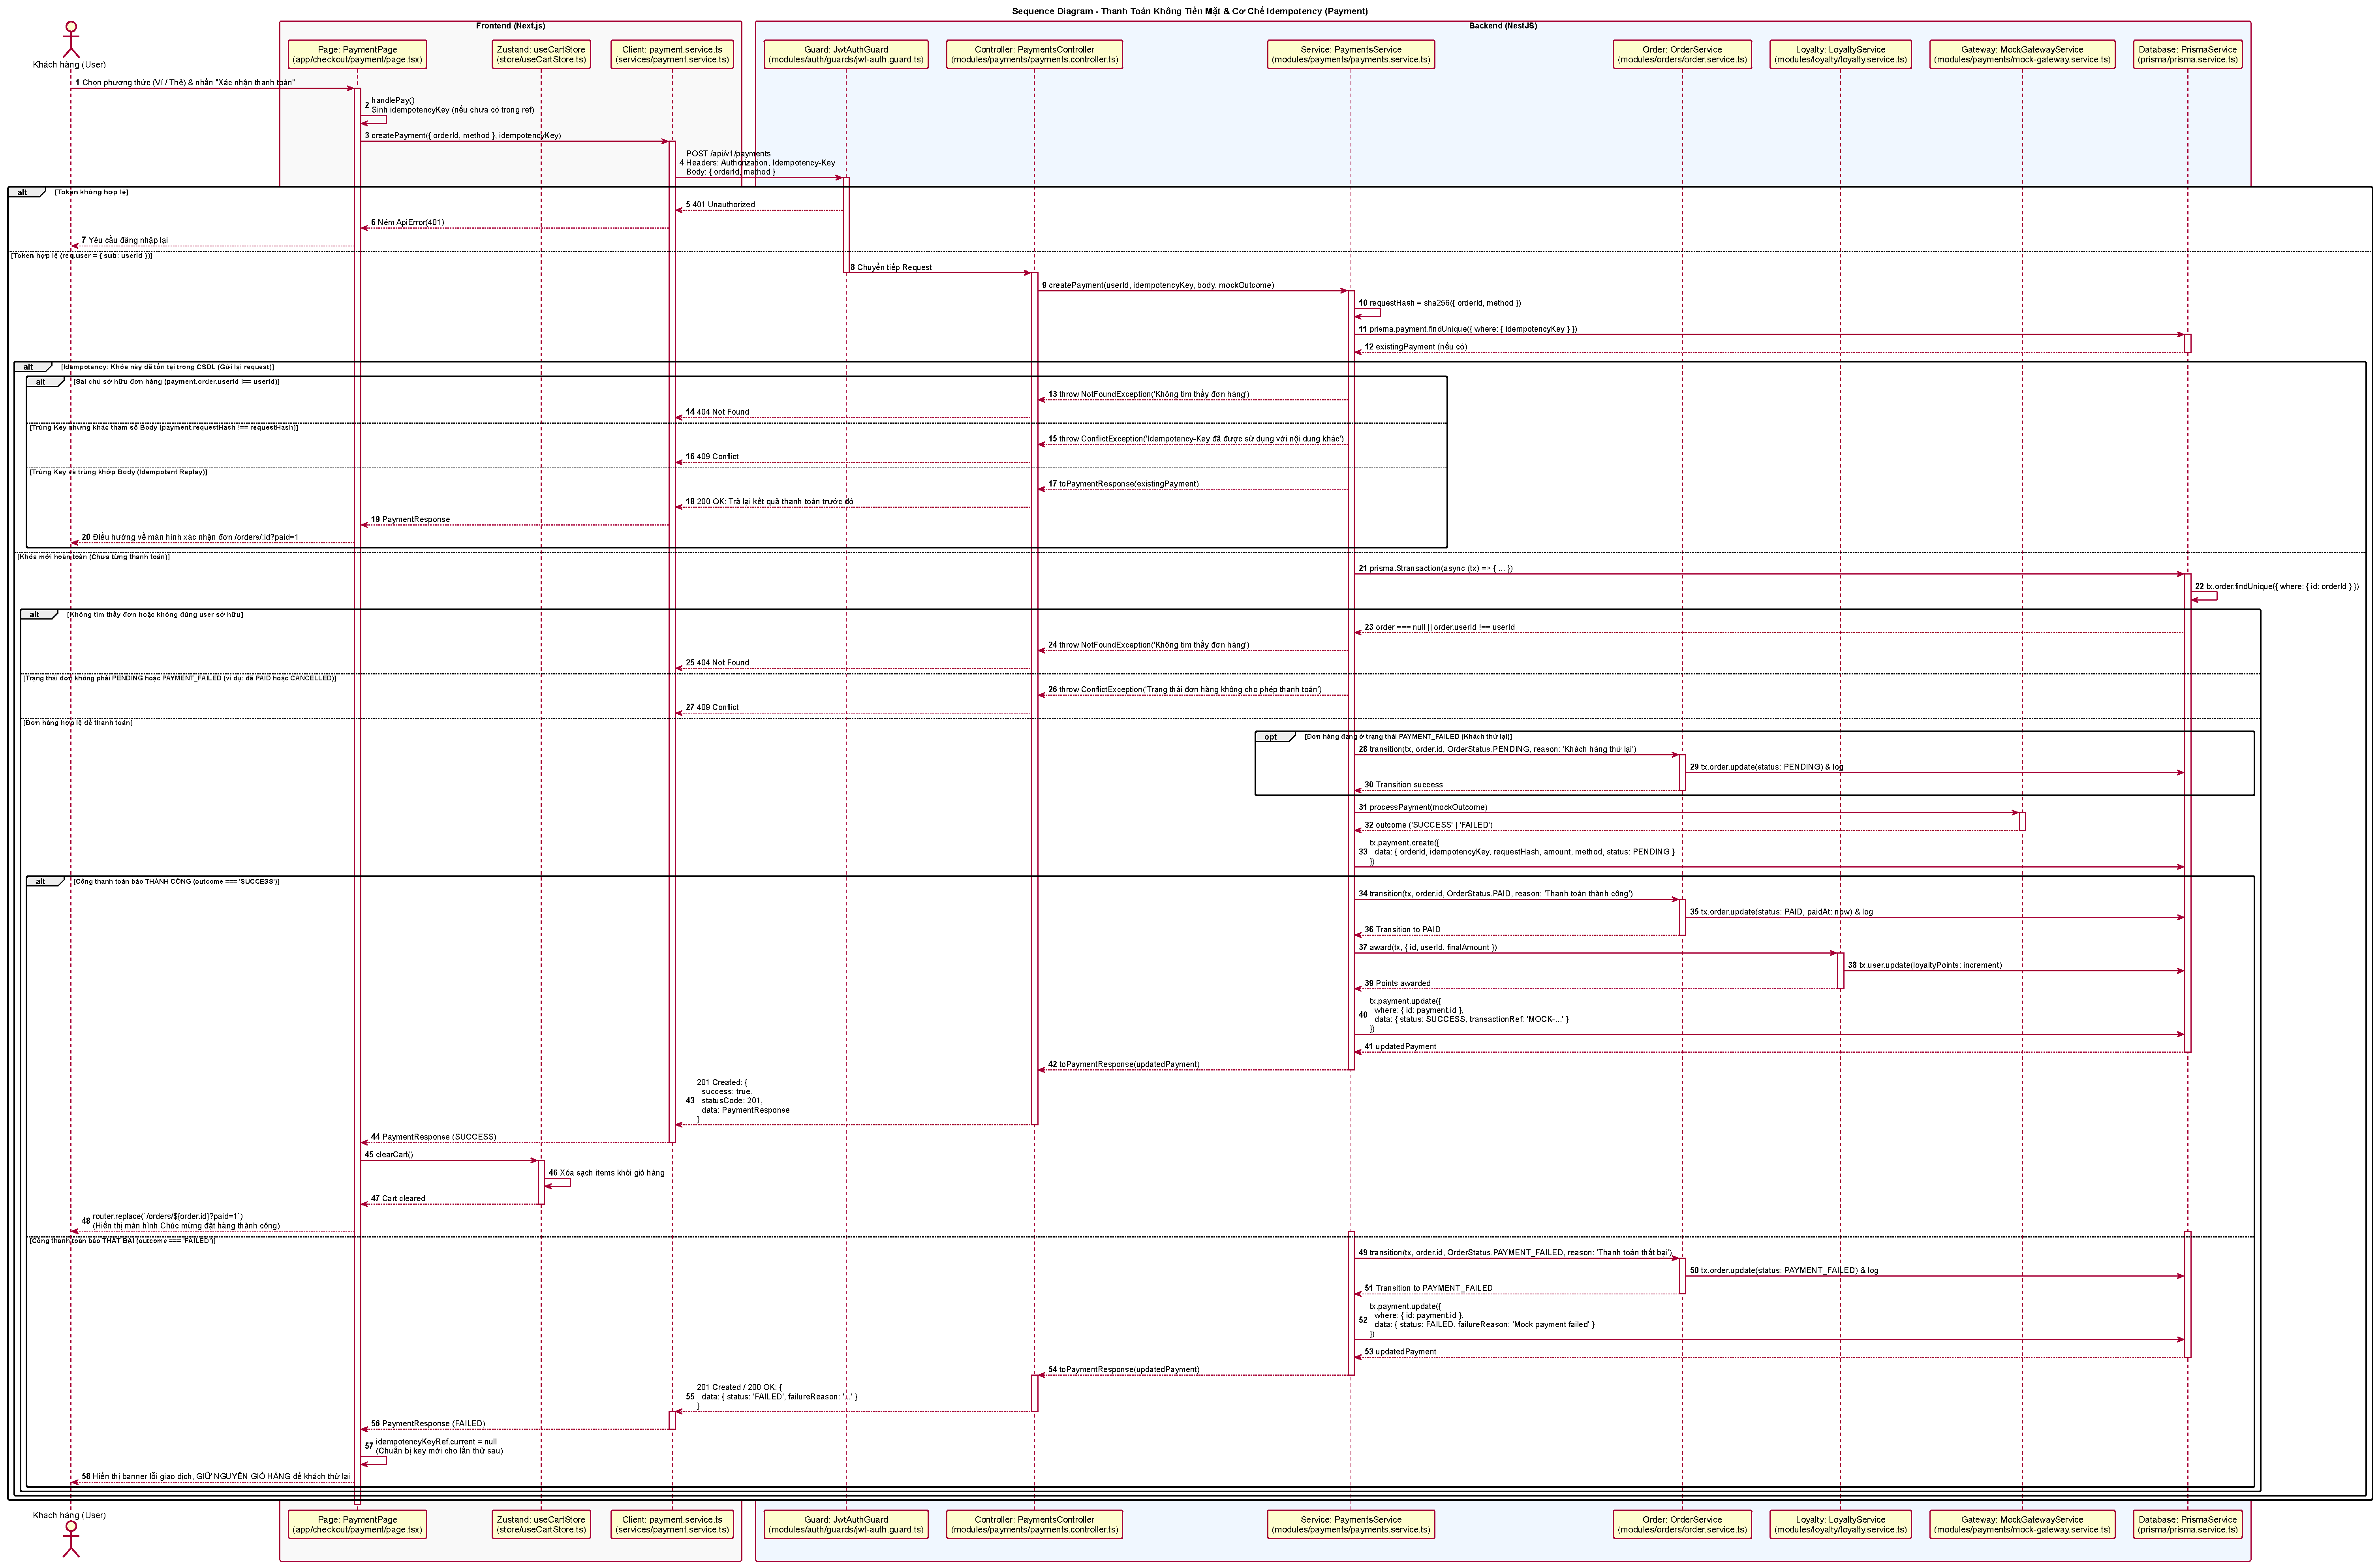
\includegraphics[width=\textwidth, height=0.80\textheight, keepaspectratio]{figures/sequence-payment.pdf}
    \caption{Sơ đồ Tuần tự - Phân hệ Thanh toán (Idempotent Flow \& Gateway Integration)}
    \label{fig:sequence-payment}
\end{figure}

\clearpage
\subsection{Hợp đồng API (API Contract)}
\begin{table}[H]
\centering
\small
\caption{Danh mục API Endpoints - Phân hệ Thanh toán}
\label{tab:api-payment}
\begin{tabularx}{\textwidth}{llp{4.5cm}X}
\toprule
\textbf{Phương thức} & \textbf{Endpoint} & \textbf{Headers \& Body} & \textbf{Phản hồi chính} \\
\midrule
\texttt{POST} & \texttt{/api/v1/payments} & 
Header: \texttt{Idempotency-Key: <UUID>}, Bearer Token.\newline Body: \texttt{\{orderId, method\}} & 
\texttt{200 OK}: Trả về chi tiết thanh toán thành công (hoặc kết quả phát lại). Lỗi: \texttt{400 Bad Request}, \texttt{401 Unauthorized}, \texttt{404 Not Found}, \texttt{409 Conflict} (sai lệch requestHash hoặc trạng thái đơn không hợp lệ). \\
\texttt{GET} & \texttt{/api/v1/payments/:id} & Tham số \texttt{id} bản ghi thanh toán & 
\texttt{200 OK}: Tra cứu trạng thái giao dịch thanh toán hiện tại. \\
\bottomrule
\end{tabularx}
\end{table}

\subsection{Ánh xạ Cơ sở dữ liệu (Database Mapping)}
\begin{itemize}
    \item \textbf{Cơ chế Idempotency:} Bảng \texttt{payments} sử dụng ràng buộc \texttt{@unique} trên trường \texttt{idempotency\_key} kết hợp cùng \texttt{request\_hash} sinh từ thuật toán SHA-256 trên nội dung JSON của body request:
    \begin{lstlisting}[language=SQL]
SELECT id, status, request_hash, transaction_ref 
FROM payments 
WHERE idempotency_key = :idempotencyKey;
    \end{lstlisting}
    \item \textbf{Cập nhật sau thanh toán thành công:} Thực thi trong transaction cập nhật đồng thời 4 bảng:
    \begin{lstlisting}[language=SQL]
UPDATE payments SET status = 'SUCCESS', transaction_ref = :ref WHERE id = :paymentId;
UPDATE orders SET status = 'PAID', paid_at = NOW() WHERE id = :orderId;
UPDATE users SET loyalty_points = loyalty_points + :pointsEarned WHERE id = :userId;
INSERT INTO loyalty_transactions (id, user_id, order_id, points, type, reason, created_at)
VALUES (cuid(), :userId, :orderId, :pointsEarned, 'EARNED', 'Tich diem tu don hang', NOW());
INSERT INTO order_status_history (id, order_id, from_status, to_status, changed_by, created_at)
VALUES (cuid(), :orderId, 'PENDING', 'PAID', 'payment_gateway', NOW());
    \end{lstlisting}
\end{itemize}

\subsection{Kịch bản Kiểm thử (Test Cases)}
\begin{table}[H]
\centering
\small
\caption{Tóm lược các Ca kiểm thử tiêu biểu - Phân hệ Thanh toán}
\label{tab:tc-payment}
\begin{tabularx}{\textwidth}{llp{2.6cm}p{3cm}Xc}
\toprule
\textbf{Mã TC} & \textbf{Loại} & \textbf{Tiền điều kiện} & \textbf{Endpoint / Màn hình} & \textbf{Kết quả mong đợi} & \textbf{Trạng thái} \\
\midrule
\texttt{TC-PAY-API-01} & Hợp lệ & Đơn PENDING, key mới & \texttt{POST /payments} & HTTP 200, status SUCCESS, đơn chuyển sang PAID & Chưa chạy \\
\texttt{TC-PAY-API-03} & Idempotent & Gửi lại cùng key & \texttt{POST /payments} & HTTP 200, trả về kết quả cũ, không gọi lại gateway & Chưa chạy \\
\texttt{TC-PAY-API-05} & Lỗi & Đơn đã thanh toán & \texttt{POST /payments} & HTTP 400, báo lỗi đơn hàng đã thanh toán & Chưa chạy \\
\texttt{TC-PAY-UI-01} & Giao diện & Đơn hàng chờ & Trang \texttt{/payment/[id]} & Hiển thị tổng tiền và 2 phương thức thẻ/ví & Chưa chạy \\
\bottomrule
\end{tabularx}
\end{table}

\subsection{Giao diện Người dùng}
\begin{figure}[H]
    \centering
    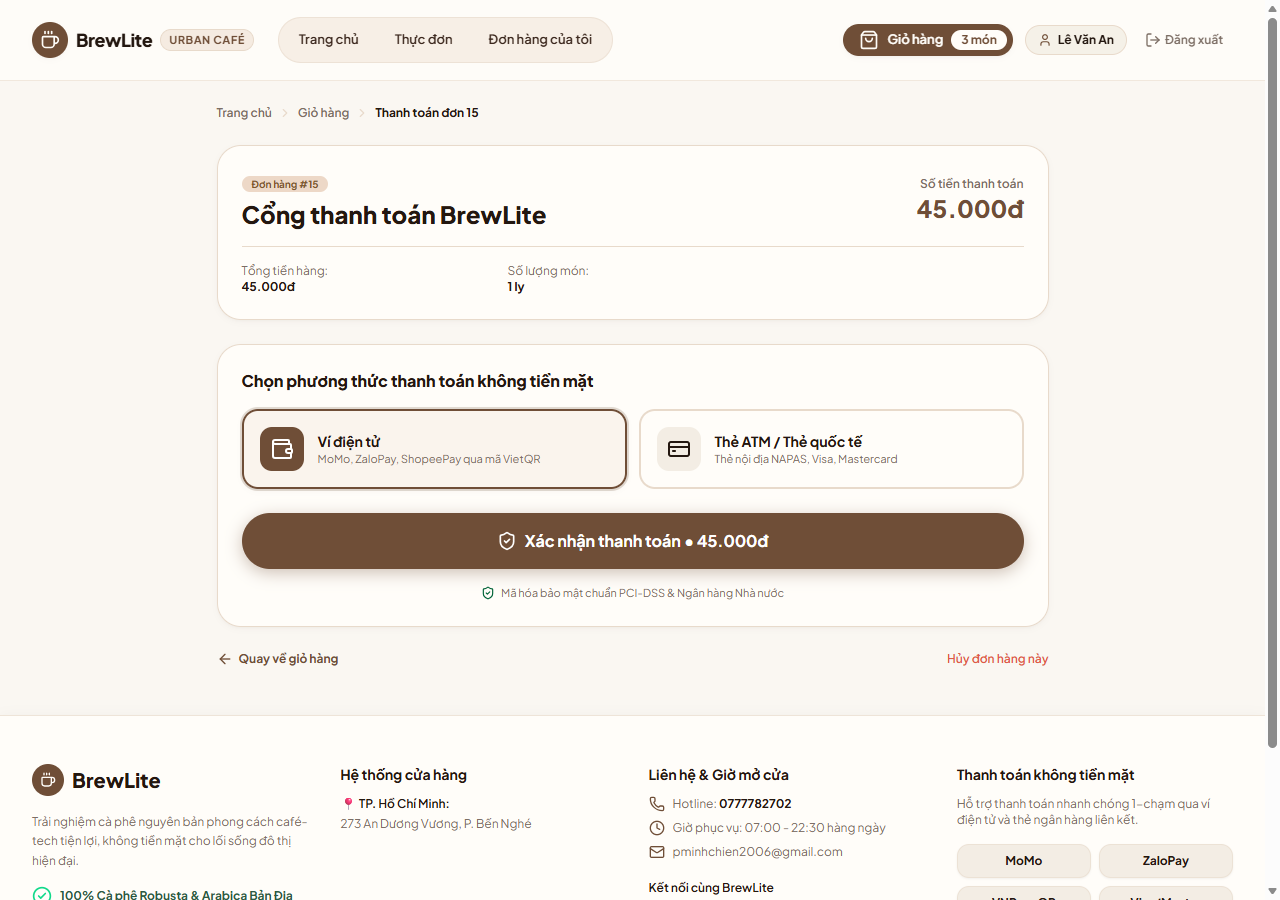
\includegraphics[width=0.92\textwidth]{figures/ui-payment.png}
    \caption{Giao diện Cổng thanh toán không tiền mặt đa phương thức}
    \label{fig:ui-payment}
\end{figure}

% ====== END INLINE: chapters/feature-payment ======


% ====== BEGIN INLINE: chapters/feature-history ======
\clearpage
\section{Phân hệ Lịch sử Đơn hàng (Order History)}

\subsection{Đặc tả Use Case}
Phân hệ Lịch sử Đơn hàng cho phép khách hàng tra cứu toàn bộ các đơn hàng đã đặt trong quá khứ, theo dõi trạng thái pha chế và kiểm tra hóa đơn chi tiết. Sơ đồ Use Case được minh họa tại Hình~\ref{fig:usecase-order-history}.

\begin{figure}[H]
    \centering
    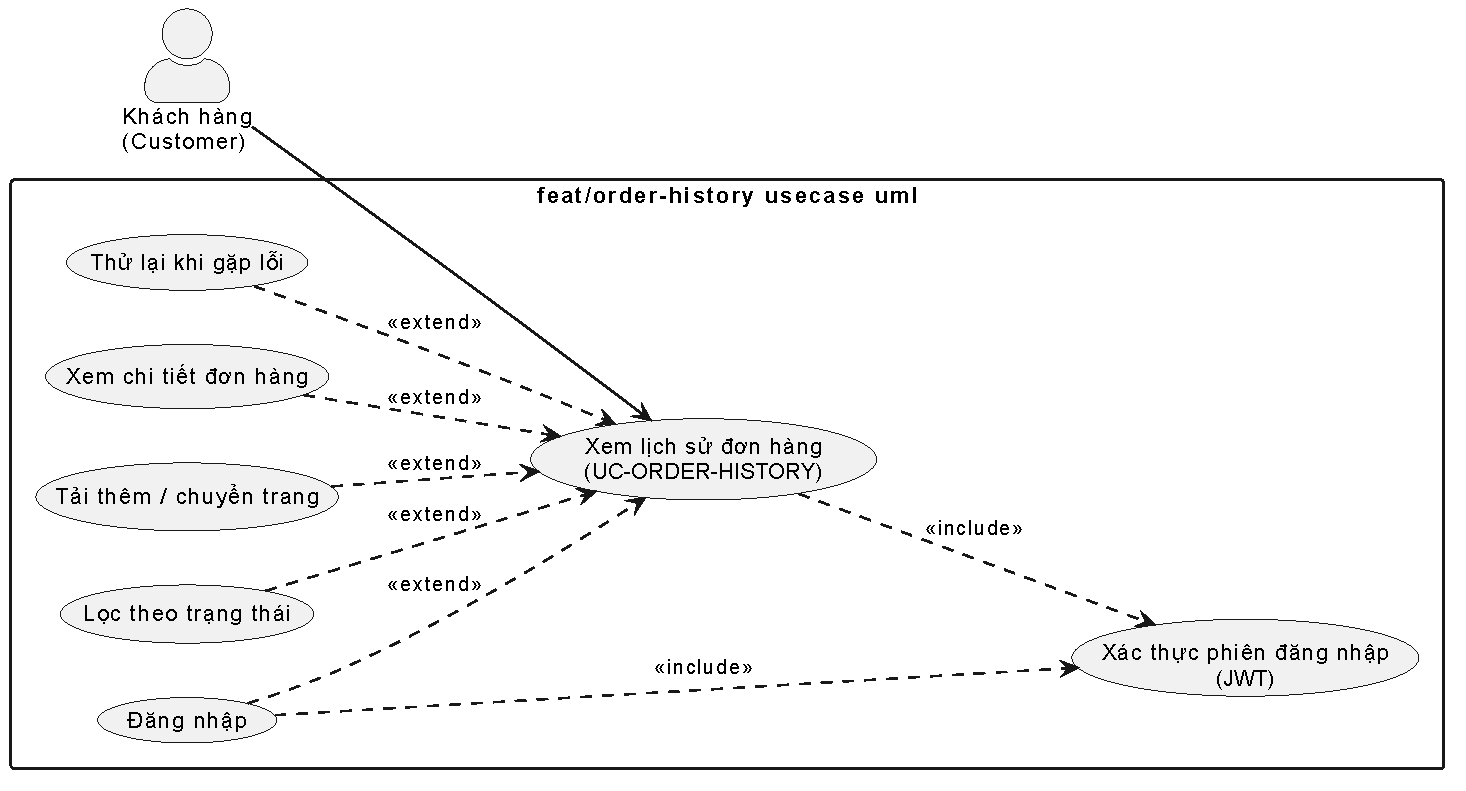
\includegraphics[width=0.75\textwidth]{figures/usecase-order-history.pdf}
    \caption{Sơ đồ Use Case - Phân hệ Lịch sử Đơn hàng}
    \label{fig:usecase-order-history}
\end{figure}

\begin{table}[H]
\centering
\small
\caption{Đặc tả Use Case: Tra cứu Lịch sử và Chi tiết Đơn hàng (UC-HIS-01)}
\label{tab:uc-spec-history}
\begin{tabularx}{\textwidth}{p{2.8cm}X}
\toprule
\textbf{Mục} & \textbf{Chi tiết Đặc tả} \\
\midrule
\textbf{Actor} & Khách hàng đã đăng nhập \\
\midrule
\textbf{Tiền điều kiện} & Khách hàng đã đăng nhập vào hệ thống. \\
\midrule
\textbf{Hậu điều kiện} & Danh sách các đơn hàng và trạng thái chi tiết hiển thị trực quan. \\
\midrule
\textbf{Luồng chính} & 
1. Khách hàng nhấp vào mục "Lịch sử đơn hàng" trên thanh điều hướng hoặc truy cập \texttt{/orders}.\newline
2. Giao diện gửi request \texttt{GET /api/v1/orders} kèm Bearer Token.\newline
3. Backend truy vấn các đơn hàng thuộc về \texttt{userId} hiện tại, sắp xếp giảm dần theo thời gian tạo (\texttt{createdAt desc}).\newline
4. Màn hình hiển thị danh sách các thẻ đơn hàng: mã hiển thị \texttt{\#orderNumber}, ngày giờ đặt, tổng tiền, huy hiệu trạng thái (ví dụ "Đã thanh toán", "Đã hủy").\newline
5. Khách hàng nhấp vào một đơn hàng để xem chi tiết hóa đơn (\texttt{/orders/[id]}): danh sách từng món, size, topping, số tiền giảm giá và phương thức thanh toán. \\
\midrule
\textbf{Luồng ngoại lệ} & 
- Người dùng chưa có đơn hàng nào: Giao diện hiển thị thông báo "Bạn chưa có đơn hàng nào" và nút liên kết "Bắt đầu đặt món".\newline
- Phiên đăng nhập hết hạn: Báo lỗi \texttt{401 Unauthorized}, tự động chuyển hướng về trang đăng nhập. \\
\bottomrule
\end{tabularx}
\end{table}

\clearpage
\subsection{Sơ đồ Hoạt động (Activity Diagram)}
Quy trình truy vấn danh sách và xem chi tiết trạng thái đơn hàng được thể hiện tại Hình~\ref{fig:activity-order-history}.

\begin{figure}[H]
    \centering
    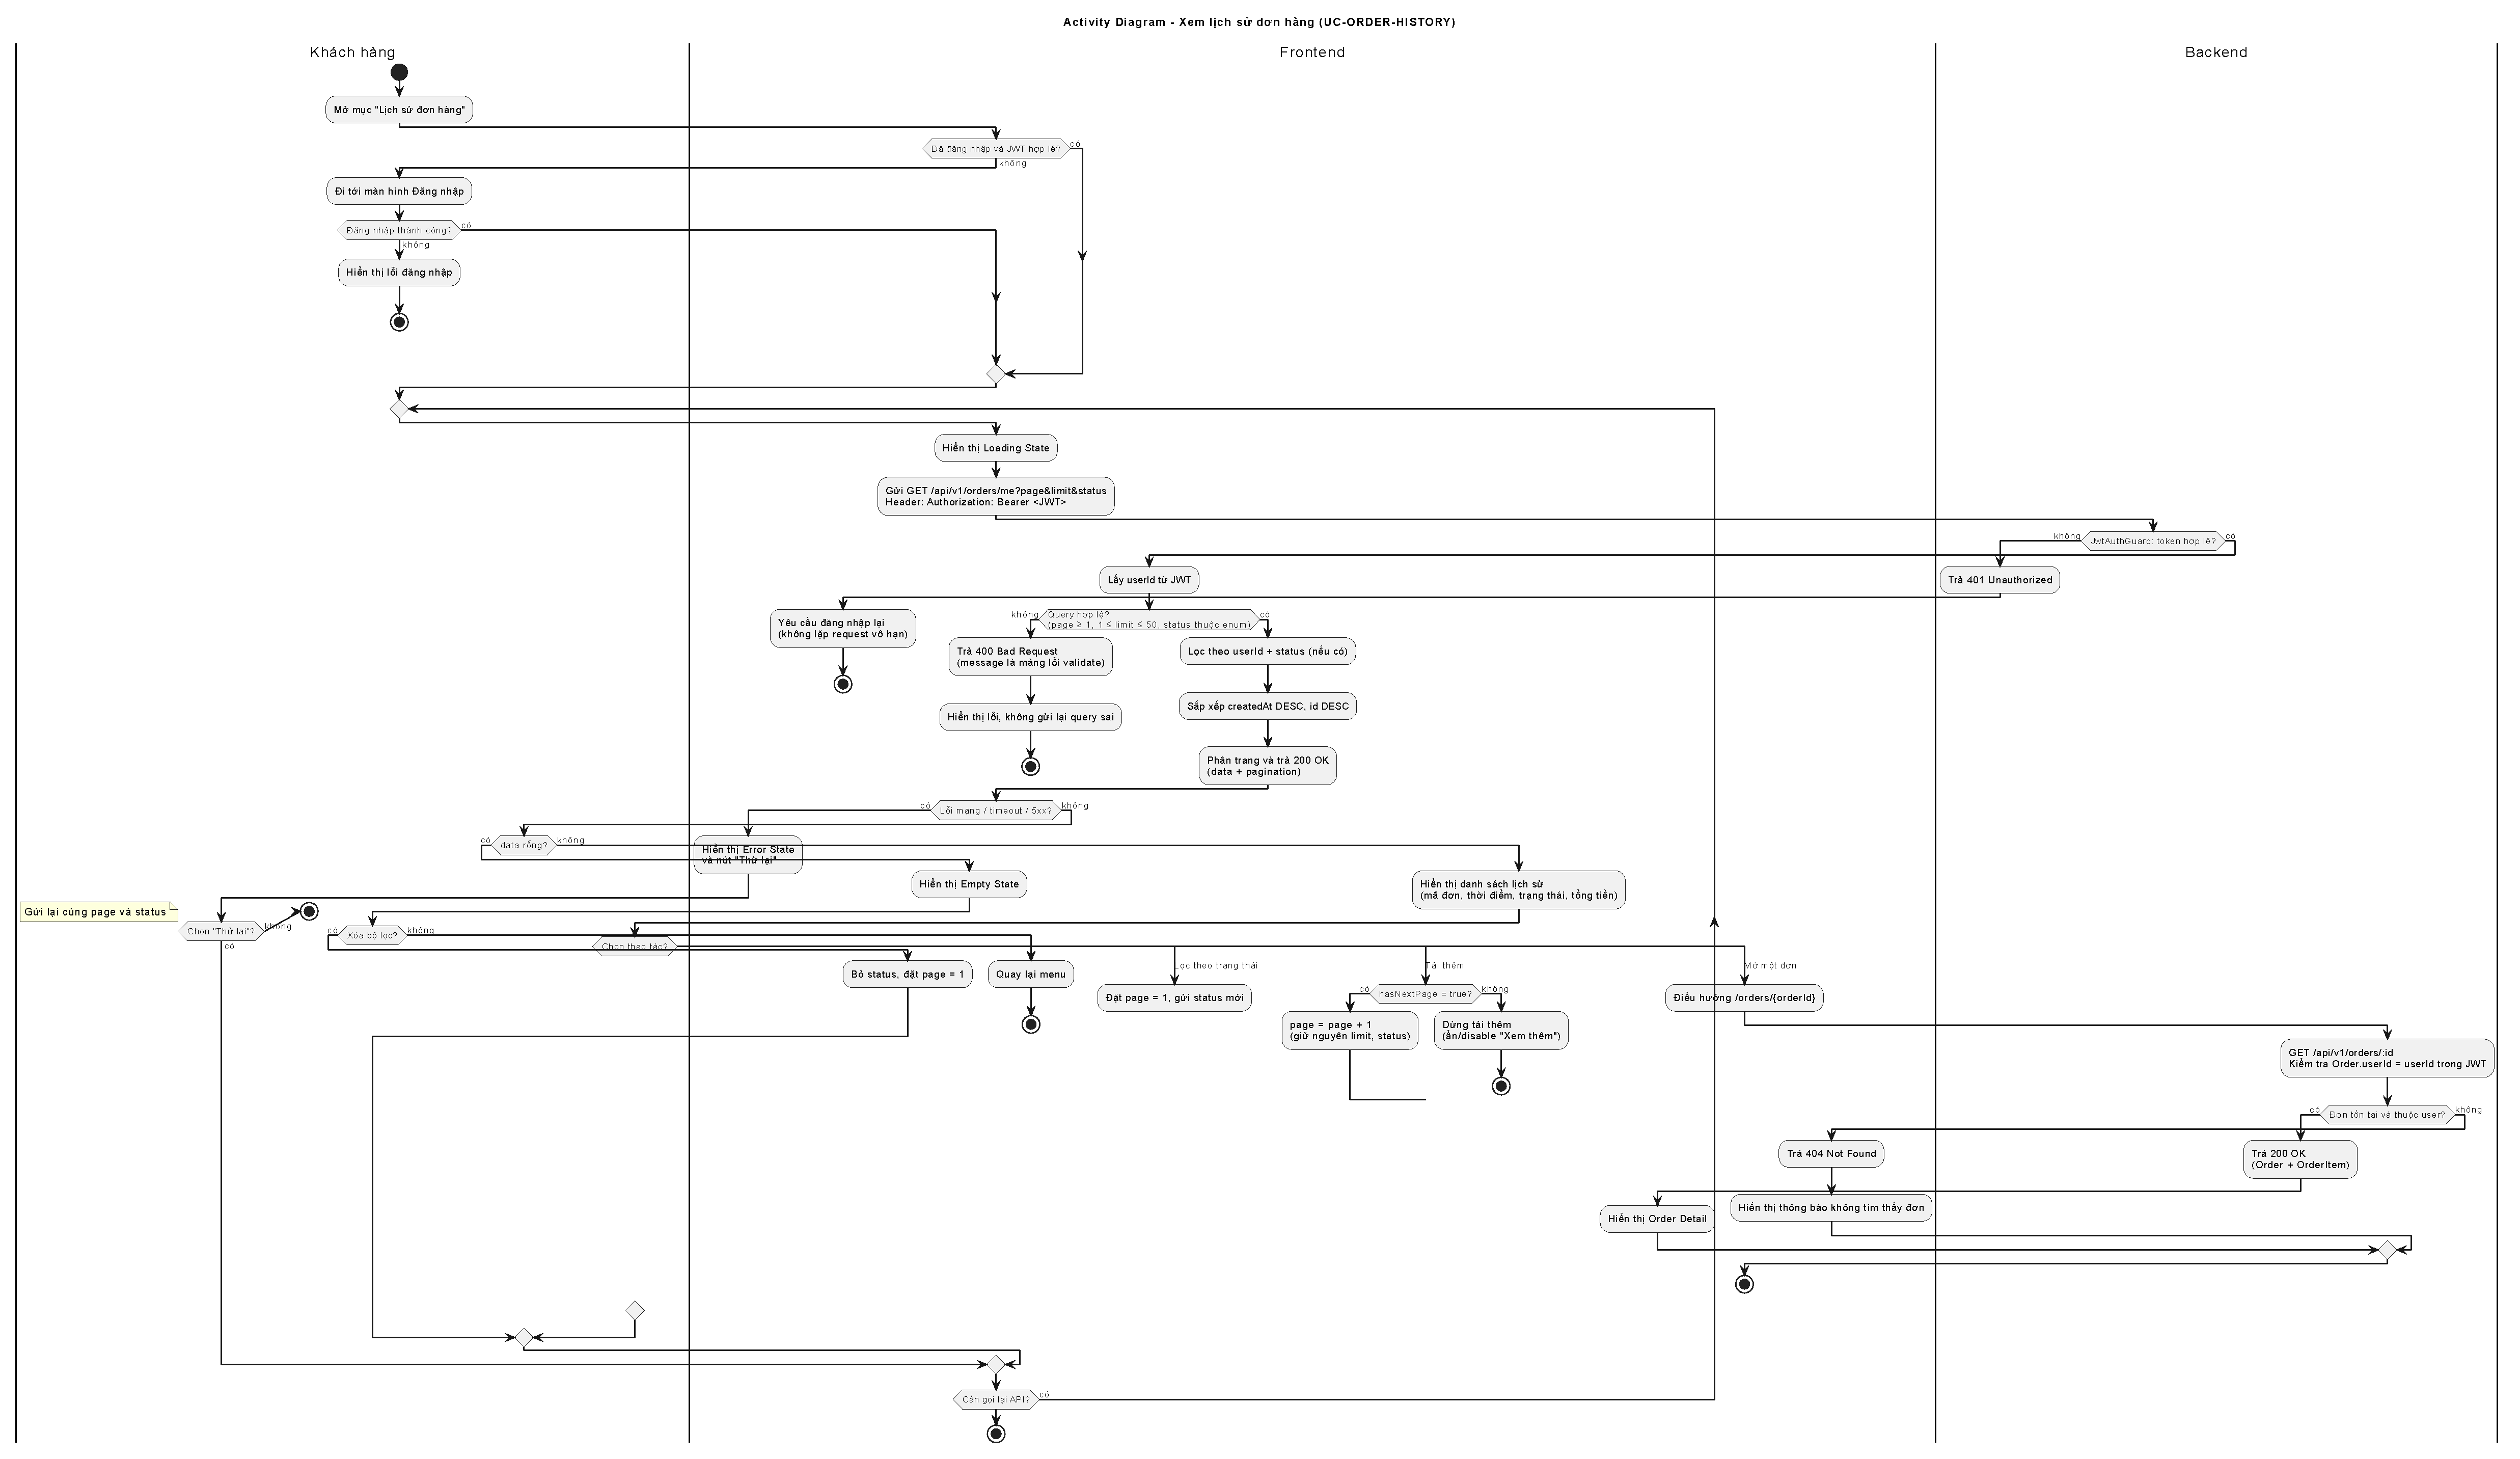
\includegraphics[width=\textwidth, height=0.80\textheight, keepaspectratio]{figures/activity-order-history.pdf}
    \caption{Sơ đồ Hoạt động - Phân hệ Lịch sử Đơn hàng}
    \label{fig:activity-order-history}
\end{figure}

\clearpage
\subsection{Sơ đồ Tuần tự (Sequence Diagram)}
Sơ đồ Tuần tự minh họa tương tác nạp dữ liệu lịch sử đơn hàng từ Frontend đến Controller, Service và Prisma tại Hình~\ref{fig:sequence-order-history}.

\begin{figure}[H]
    \centering
    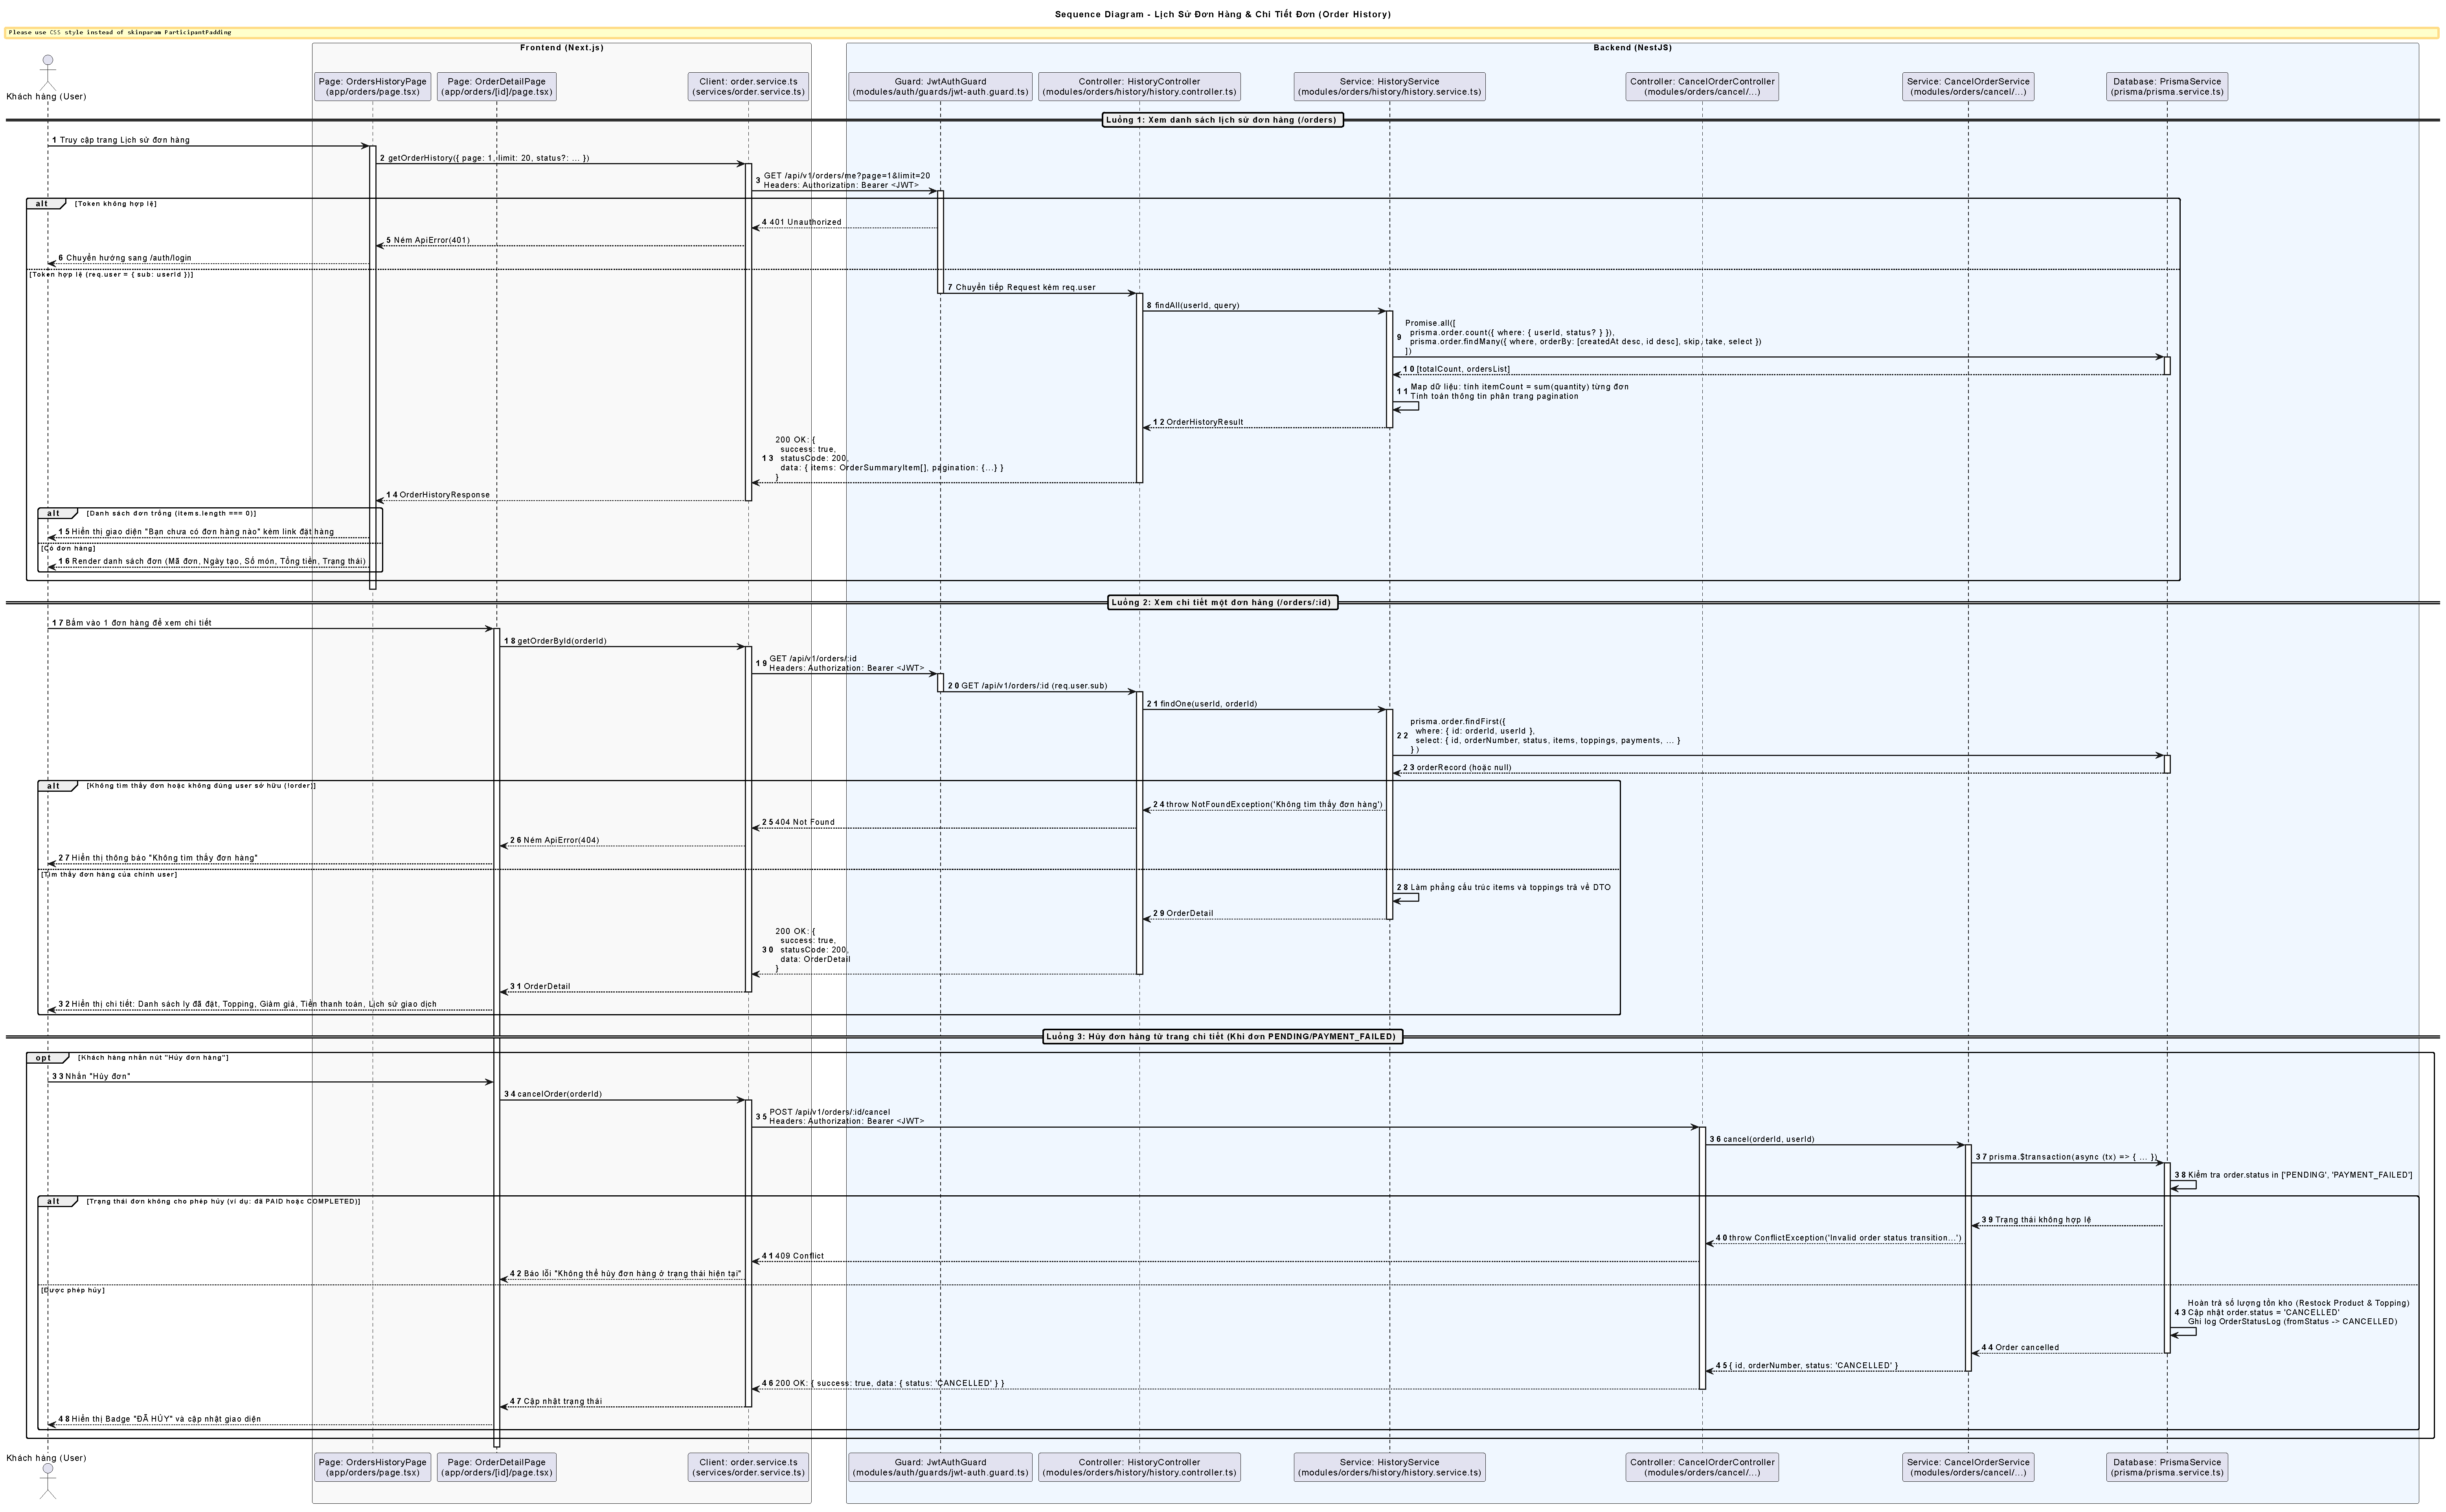
\includegraphics[width=\textwidth, height=0.80\textheight, keepaspectratio]{figures/sequence-order-history.pdf}
    \caption{Sơ đồ Tuần tự - Phân hệ Lịch sử Đơn hàng}
    \label{fig:sequence-order-history}
\end{figure}

\clearpage
\subsection{Hợp đồng API (API Contract)}
\begin{table}[H]
\centering
\small
\caption{Danh mục API Endpoints - Phân hệ Lịch sử Đơn hàng}
\label{tab:api-history}
\begin{tabularx}{\textwidth}{llp{4cm}X}
\toprule
\textbf{Phương thức} & \textbf{Endpoint} & \textbf{Header} & \textbf{Phản hồi chính} \\
\midrule
\texttt{GET} & \texttt{/api/v1/orders} & \texttt{Authorization: Bearer <JWT>} & \texttt{200 OK}: Danh sách các đơn hàng của user đang đăng nhập, kèm tổng tiền và trạng thái. \\
\texttt{GET} & \texttt{/api/v1/orders/:id} & \texttt{Authorization: Bearer <JWT>} & \texttt{200 OK}: Chi tiết đơn hàng gồm các món (\texttt{items}), topping và lịch sử trạng thái (\texttt{statusHistory}). Lỗi \texttt{404} nếu không tìm thấy hoặc không thuộc sở hữu. \\
\bottomrule
\end{tabularx}
\end{table}

\subsection{Ánh xạ Cơ sở dữ liệu (Database Mapping)}
\begin{itemize}
    \item Truy vấn danh sách đơn hàng cá nhân:
    \begin{lstlisting}[language=SQL]
SELECT id, order_number, status, total_amount, discount_amount, final_amount, created_at 
FROM orders 
WHERE user_id = :userId 
ORDER BY created_at DESC;
    \end{lstlisting}
    \item Tối ưu hóa: Chỉ mục \texttt{@@index([userId])} và \texttt{@@index([status])} trên bảng \texttt{orders} đảm bảo câu truy vấn thực thi với độ phức tạp \(\mathcal{O}(\log N)\), đáp ứng yêu cầu phản hồi nhanh của hệ thống.
\end{itemize}

\subsection{Kịch bản Kiểm thử (Test Cases)}
\begin{table}[H]
\centering
\small
\caption{Tóm lược các Ca kiểm thử tiêu biểu - Phân hệ Lịch sử}
\label{tab:tc-history}
\begin{tabularx}{\textwidth}{llp{2.6cm}p{3cm}Xc}
\toprule
\textbf{Mã TC} & \textbf{Loại} & \textbf{Tiền điều kiện} & \textbf{Endpoint / Màn hình} & \textbf{Kết quả mong đợi} & \textbf{Trạng thái} \\
\midrule
\texttt{TC-HIS-API-01} & Hợp lệ & User có 3 đơn hàng & \texttt{GET /orders} & HTTP 200, trả về đủ 3 đơn sắp xếp mới nhất & Chưa chạy \\
\texttt{TC-HIS-API-02} & Bảo mật & Xem đơn của user khác & \texttt{GET /orders/:id} & HTTP 404 hoặc 403, không lộ đơn của người khác & Chưa chạy \\
\texttt{TC-HIS-UI-01} & Giao diện & User chưa có đơn nào & Màn hình \texttt{/orders} & Hiển thị chuỗi "Bạn chưa có đơn hàng nào" & Chưa chạy \\
\texttt{TC-HIS-UI-03} & Giao diện & Đơn đã bị hủy & Danh sách đơn & Hiển thị đúng badge trạng thái "Đã hủy" & Chưa chạy \\
\bottomrule
\end{tabularx}
\end{table}

\subsection{Giao diện Người dùng}
\begin{figure}[H]
    \centering
    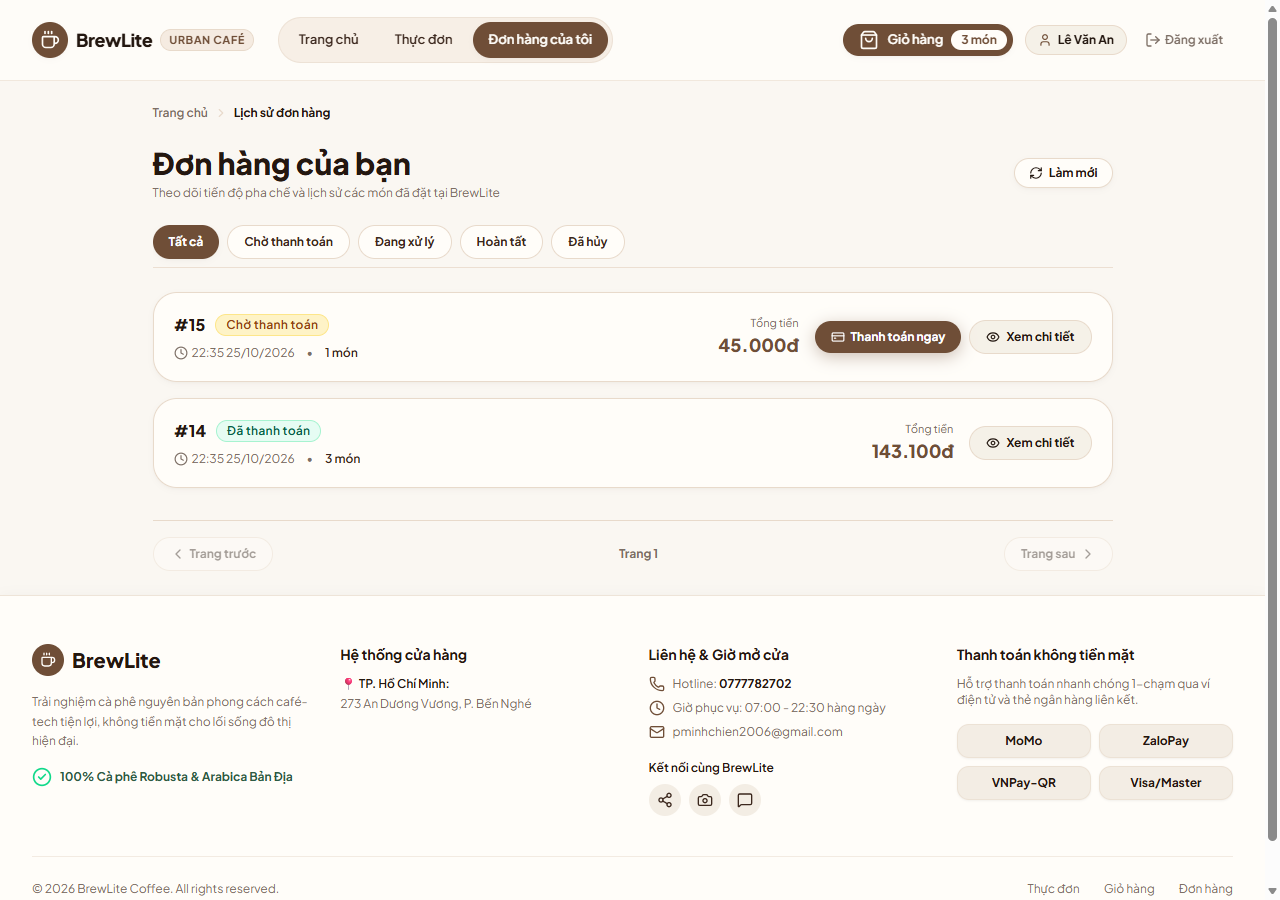
\includegraphics[width=0.92\textwidth]{figures/ui-history.png}
    \caption{Giao diện Lịch sử và Trạng thái Đơn hàng của Khách hàng}
    \label{fig:ui-history}
\end{figure}

% ====== END INLINE: chapters/feature-history ======

\section{Phân hệ Xác thực Người dùng (Auth)}

\subsection{Đặc tả Use Case}
Phân hệ Xác thực quản lý vòng đời tài khoản của người dùng, cung cấp cơ chế đăng ký và đăng nhập bảo mật bằng JSON Web Token (JWT). Sơ đồ Use Case được minh họa tại Hình~\ref{fig:usecase-auth}.

\begin{figure}[htbp]
    \centering
    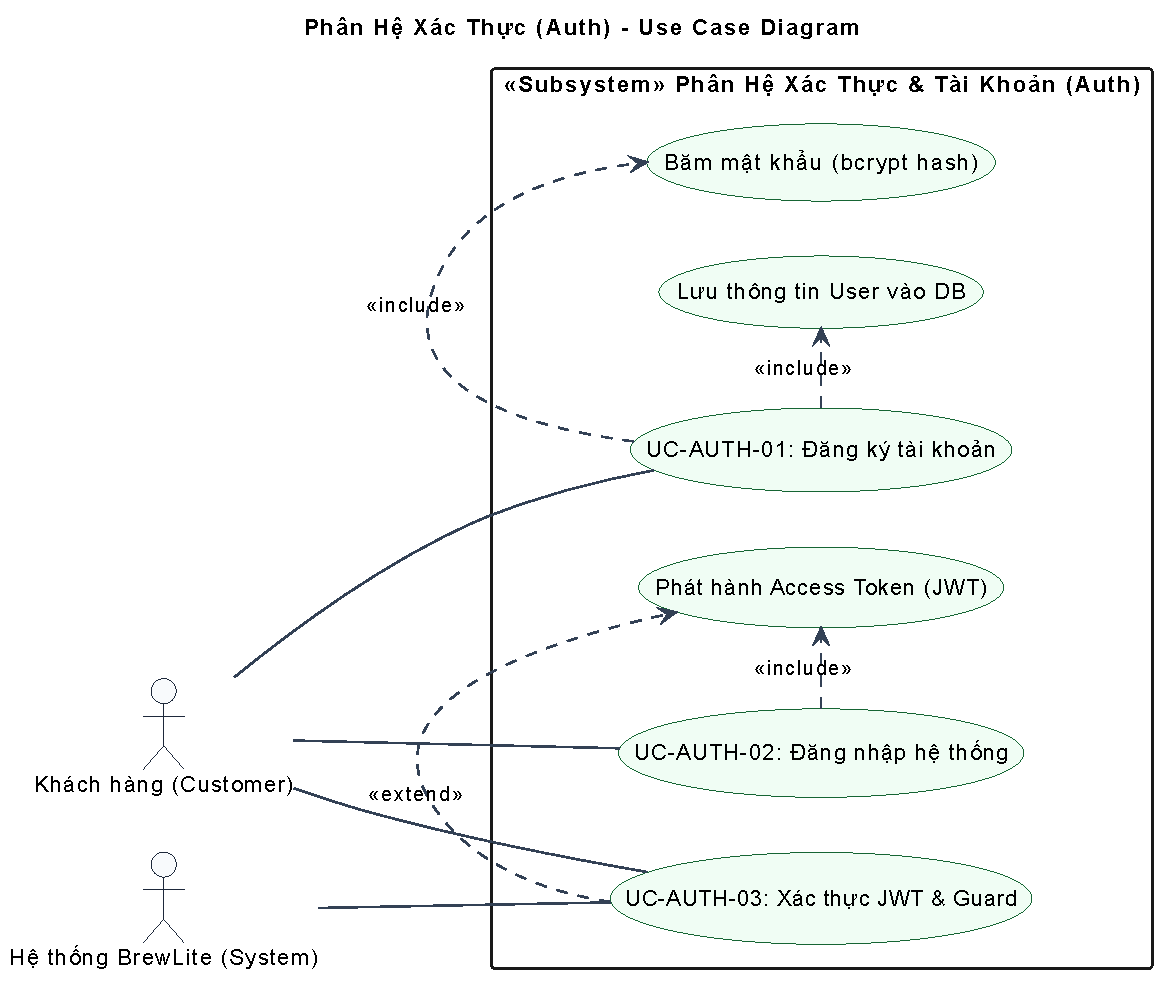
\includegraphics[width=0.75\textwidth]{figures/usecase-auth.pdf}
    \caption{Sơ đồ Use Case - Phân hệ Xác thực}
    \label{fig:usecase-auth}
\end{figure}

\begin{table}[htbp]
\centering
\small
\caption{Đặc tả Use Case: Đăng ký và Đăng nhập người dùng}
\label{tab:uc-spec-auth}
\begin{tabularx}{\textwidth}{p{2.3cm}XX}
\toprule
\textbf{Mục} & \textbf{Đăng ký (UC-AUTH-01)} & \textbf{Đăng nhập (UC-AUTH-02)} \\
\midrule
\textbf{Actor} & Khách vãng lai (Guest) & Khách hàng đã có tài khoản \\
\midrule
\textbf{Tiền điều kiện} & Chưa đăng nhập; địa chỉ email chưa tồn tại trên hệ thống. & Đã có tài khoản trên hệ thống; tài khoản ở trạng thái hoạt động. \\
\midrule
\textbf{Hậu điều kiện} & Bản ghi mới được tạo trong bảng \texttt{users}; mật khẩu được băm Bcrypt 10 rounds; khởi tạo 0 điểm loyalty. & Cấp phát mã thông báo JWT \texttt{accessToken}; lưu trữ tại client để xác thực các request kế tiếp. \\
\midrule
\textbf{Luồng chính} & 
1. Người dùng nhập email, mật khẩu (\(\ge\) 6 ký tự), họ tên.\newline
2. Nhấn "Đăng ký".\newline
3. Hệ thống kiểm tra hợp lệ DTO và tính duy nhất của email.\newline
4. Băm mật khẩu bằng \texttt{bcrypt.hash(password, 10)}.\newline
5. Tạo người dùng trong DB và trả về thông tin (loại trừ \texttt{password\_hash}). & 
1. Người dùng nhập email và mật khẩu.\newline
2. Nhấn "Đăng nhập".\newline
3. Hệ thống tìm người dùng theo email.\newline
4. So sánh mật khẩu bằng \texttt{bcrypt.compare(password, hash)}.\newline
5. Sinh mã JWT chứa payload \texttt{\{sub, email\}}.\newline
6. Trả về token và thông tin hồ sơ người dùng. \\
\midrule
\textbf{Luồng ngoại lệ} & 
- DTO không hợp lệ: Trả về mã \texttt{400 Bad Request}.\newline
- Trùng email: Trả về \texttt{409 Conflict} ("Email đã được sử dụng"). & 
- Email không tồn tại hoặc sai mật khẩu: Trả về \texttt{401 Unauthorized} ("Email hoặc mật khẩu không chính xác"). \\
\bottomrule
\end{tabularx}
\end{table}

\subsection{Sơ đồ Hoạt động (Activity Diagram)}
Sơ đồ Hoạt động mô tả chi tiết quy trình xử lý luồng đăng nhập và kiểm tra xác thực người dùng được biểu diễn tại Hình~\ref{fig:activity-auth}.

\begin{figure}[htbp]
    \centering
    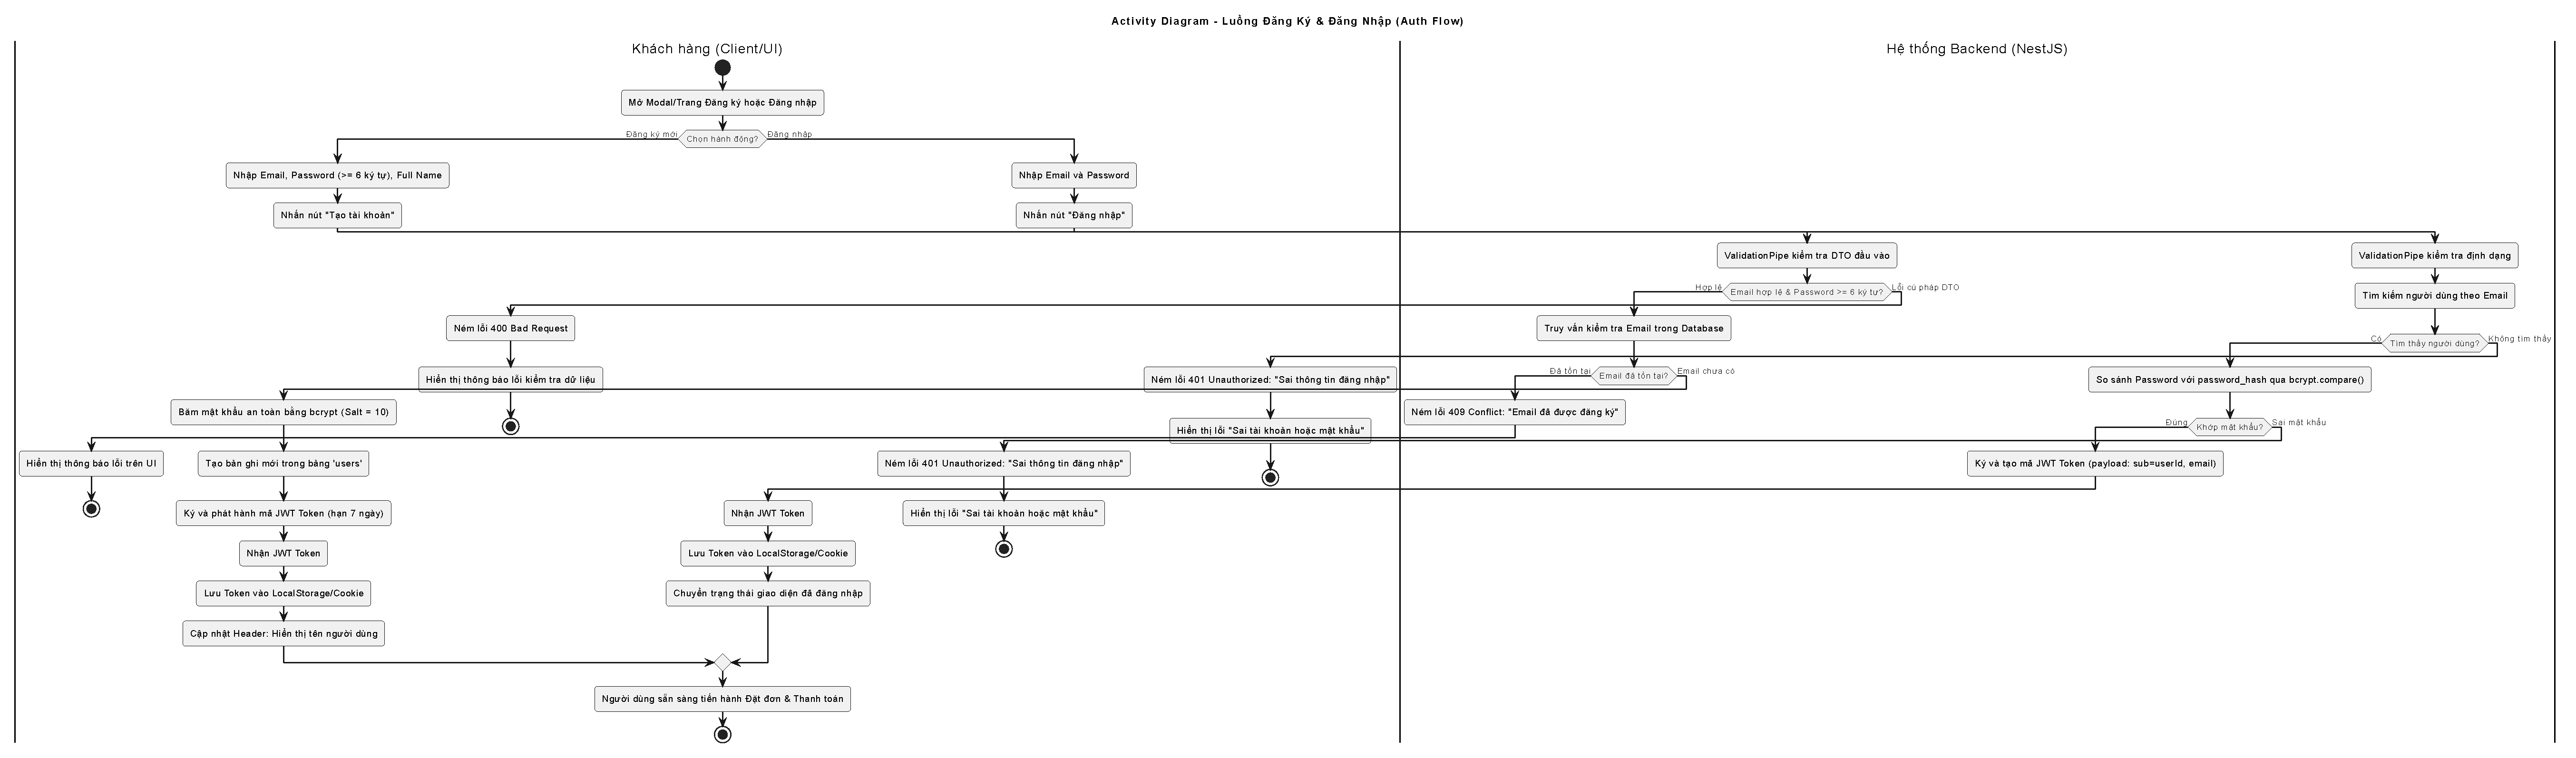
\includegraphics[width=0.75\textwidth]{figures/activity-auth.pdf}
    \caption{Sơ đồ Hoạt động - Phân hệ Xác thực}
    \label{fig:activity-auth}
\end{figure}

\subsection{Sơ đồ Tuần tự (Sequence Diagram)}
Sơ đồ Tuần tự phản ánh chuẩn xác các lời gọi hàm từ giao diện qua Controller đến Service và Prisma DB tại Hình~\ref{fig:sequence-auth}.

\begin{figure}[htbp]
    \centering
    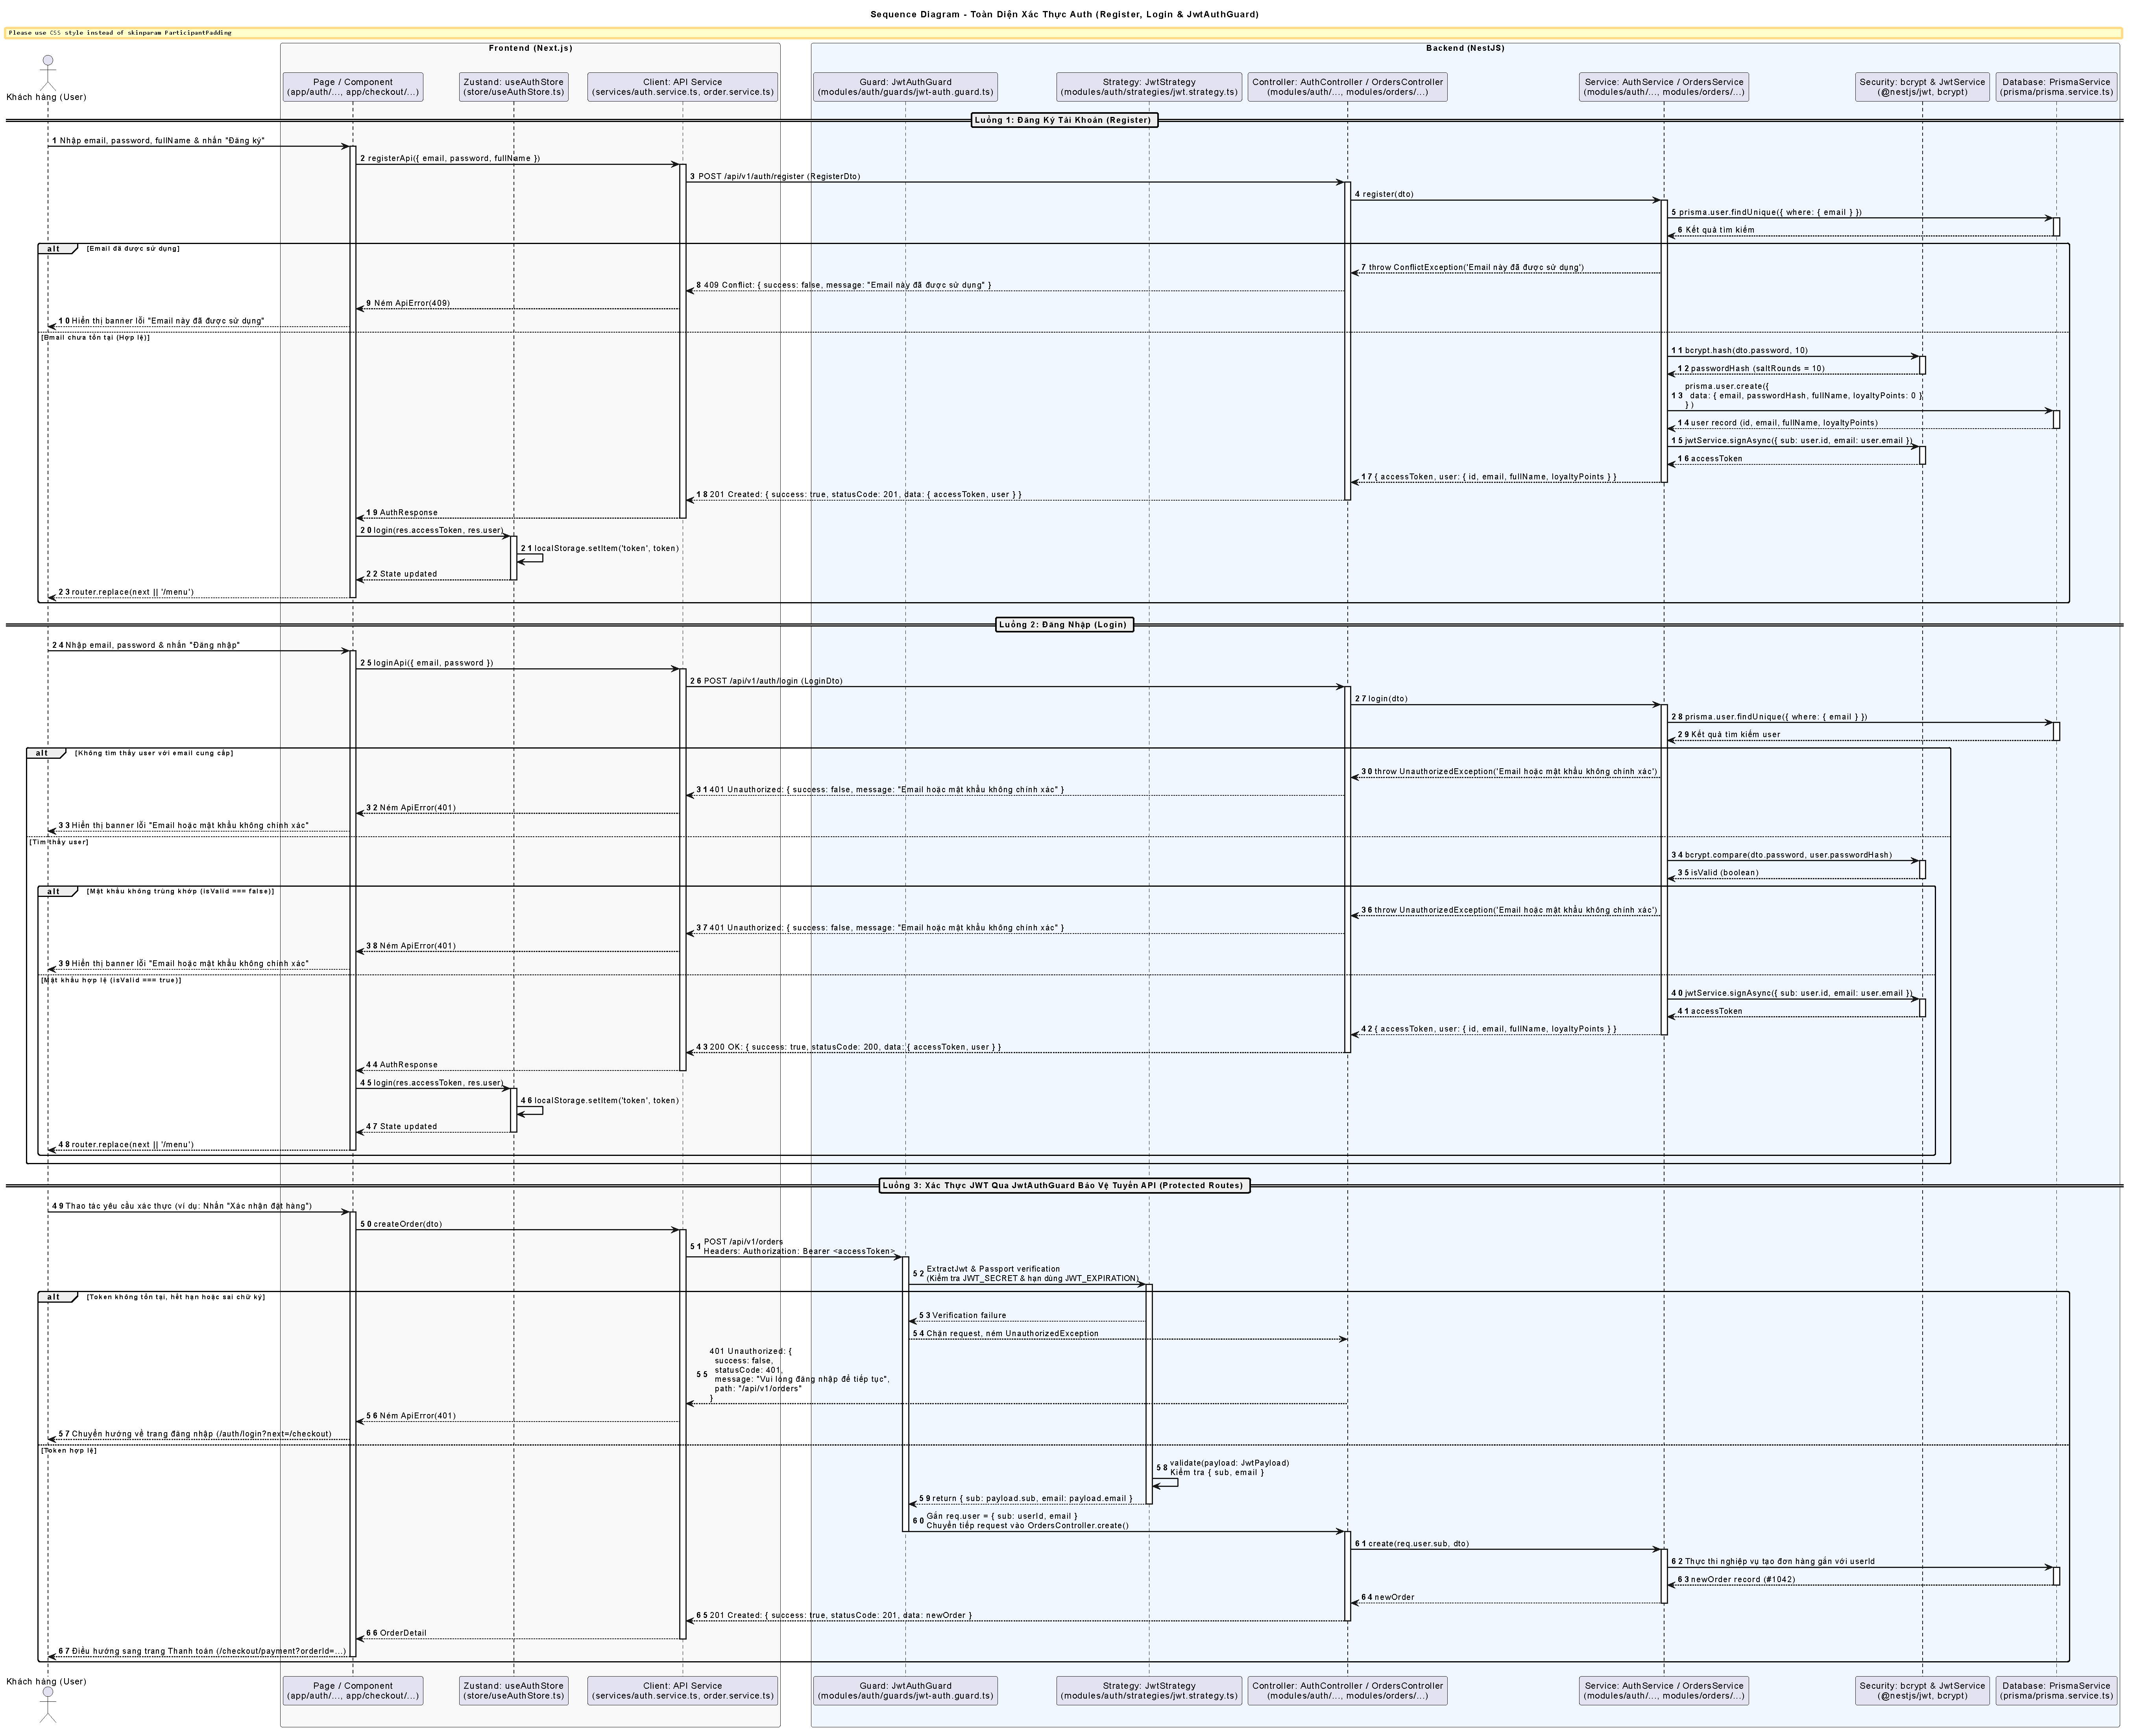
\includegraphics[width=0.9\textwidth]{figures/sequence-auth.pdf}
    \caption{Sơ đồ Tuần tự - Phân hệ Xác thực (Happy path \& Exception paths)}
    \label{fig:sequence-auth}
\end{figure}

\subsection{Hợp đồng API (API Contract)}
\begin{table}[htbp]
\centering
\small
\caption{Danh mục API Endpoints - Phân hệ Xác thực}
\label{tab:api-auth}
\begin{tabularx}{\textwidth}{llp{4cm}X}
\toprule
\textbf{Phương thức} & \textbf{Endpoint} & \textbf{Mô tả Request Body} & \textbf{Phản hồi chính} \\
\midrule
\texttt{POST} & \texttt{/api/v1/auth/register} & \texttt{\{email, password, fullName\}} (Email hợp lệ, password \(\ge 6\) ký tự) & \texttt{201 Created}: Trả về thông tin người dùng mới (loại trừ passwordHash). Lỗi: \texttt{400}, \texttt{409}. \\
\texttt{POST} & \texttt{/api/v1/auth/login} & \texttt{\{email, password\}} & \texttt{200 OK}: Trả về \texttt{accessToken} và thông tin người dùng. Lỗi: \texttt{400}, \texttt{401}. \\
\bottomrule
\end{tabularx}
\end{table}

\subsection{Ánh xạ Cơ sở dữ liệu (Database Mapping)}
Mọi thao tác của AuthModule tác động trực tiếp lên bảng \texttt{users}:
\begin{itemize}
    \item \textbf{Đăng ký:} Gọi \texttt{prisma.user.findUnique(\{ where: \{ email \} \})}. Nếu tồn tại \(\to\) throw \texttt{ConflictException}. Nếu chưa, thực thi \texttt{bcrypt.hash(password, 10)} và gọi \texttt{prisma.user.create(\{ data: \{ email, passwordHash, fullName, loyaltyPoints: 0 \} \})}.
    \item \textbf{Đăng nhập:} Gọi \texttt{prisma.user.findUnique(\{ where: \{ email \} \})}. Nếu không tìm thấy hoặc \texttt{bcrypt.compare()} trả về false \(\to\) throw \texttt{UnauthorizedException}.
    \item \textbf{Bảo mật dữ liệu:} Trường \texttt{passwordHash} tuyệt đối được lược bỏ trước khi gán vào đối tượng trả về thông qua destructuring: \texttt{const \{ passwordHash, ...userWithoutPassword \} = user}.
\end{itemize}

\subsection{Kịch bản Kiểm thử (Test Cases)}
\begin{table}[htbp]
\centering
\small
\caption{Tóm lược các Ca kiểm thử tiêu biểu - Phân hệ Xác thực}
\label{tab:tc-auth}
\begin{tabularx}{\textwidth}{llp{2.6cm}p{3cm}Xc}
\toprule
\textbf{Mã TC} & \textbf{Loại} & \textbf{Tiền điều kiện} & \textbf{Endpoint / Màn hình} & \textbf{Kết quả mong đợi} & \textbf{Trạng thái} \\
\midrule
\texttt{TC-AUTH-API-01} & Hợp lệ & Email chưa tồn tại & \texttt{POST /auth/register} & HTTP 201, tạo user mới, băm bcrypt 10 rounds & Chưa chạy \\
\texttt{TC-AUTH-API-03} & Lỗi & Email đã tồn tại & \texttt{POST /auth/register} & HTTP 409, message "Email đã được sử dụng" & Chưa chạy \\
\texttt{TC-AUTH-API-05} & Hợp lệ & Đã có tài khoản & \texttt{POST /auth/login} & HTTP 200, cấp JWT accessToken & Chưa chạy \\
\texttt{TC-AUTH-API-07} & Lỗi & Mật khẩu không đúng & \texttt{POST /auth/login} & HTTP 401, message "Email hoặc mật khẩu không chính xác" & Chưa chạy \\
\texttt{TC-AUTH-UI-01} & Giao diện & Đang ở trang \texttt{/login} & Màn hình Đăng nhập & Hiển thị form, nút "Đăng nhập", chuyển hướng thành công & Chưa chạy \\
\bottomrule
\end{tabularx}
\end{table}

\subsection{Giao diện Người dùng}
\begin{figure}[htbp]
    \centering
    \begin{subfigure}[b]{0.48\textwidth}
        \centering
        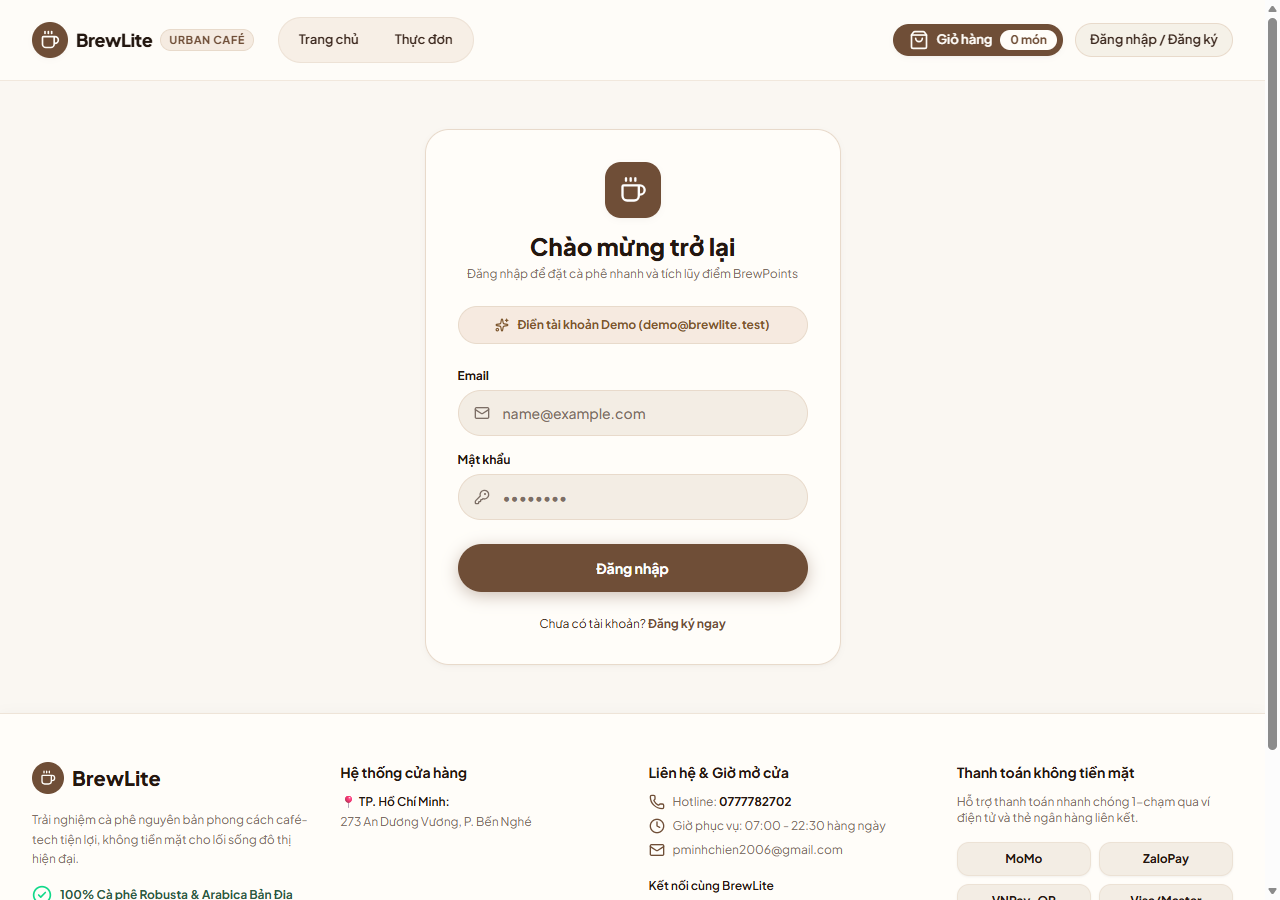
\includegraphics[width=\textwidth]{figures/ui-auth-login.png}
        \caption{Màn hình Đăng nhập}
        \label{fig:ui-auth-login}
    \end{subfigure}
    \hfill
    \begin{subfigure}[b]{0.48\textwidth}
        \centering
        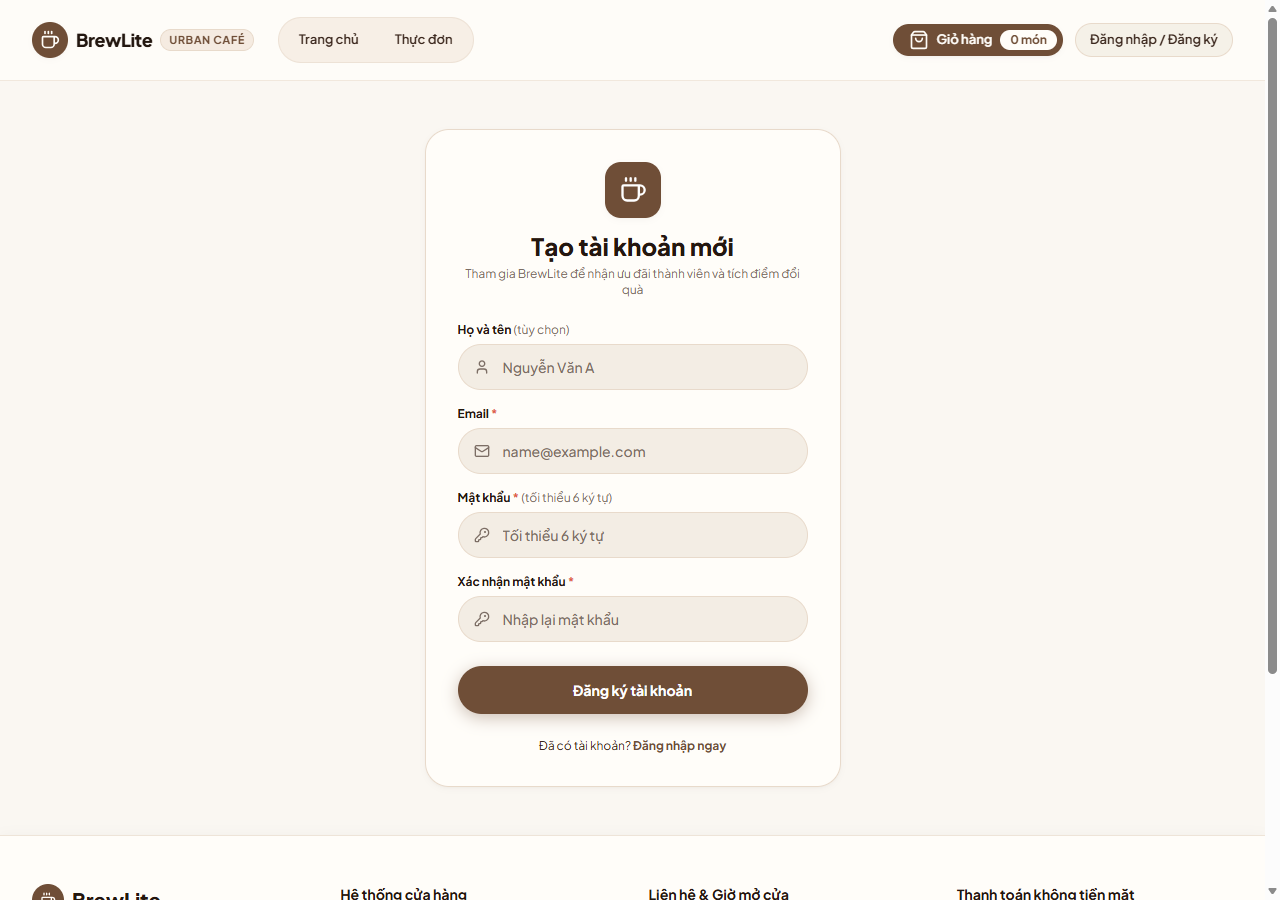
\includegraphics[width=\textwidth]{figures/ui-auth-register.png}
        \caption{Màn hình Đăng ký tài khoản}
        \label{fig:ui-auth-register}
    \end{subfigure}
    \caption{Giao diện Đăng nhập và Đăng ký người dùng}
    \label{fig:ui-auth}
\end{figure}

\clearpage
\section{Phân hệ Danh mục Sản phẩm (Product Catalog)}

\subsection{Đặc tả Use Case}
Phân hệ Danh mục Sản phẩm cho phép người dùng khám phá toàn bộ thực đơn của BrewLite, tìm kiếm đồ uống theo tên và lọc theo các phân loại như Cà phê hoặc Trà. Sơ đồ Use Case được biểu diễn tại Hình~\ref{fig:usecase-product-catalog}.

\begin{figure}[H]
    \centering
    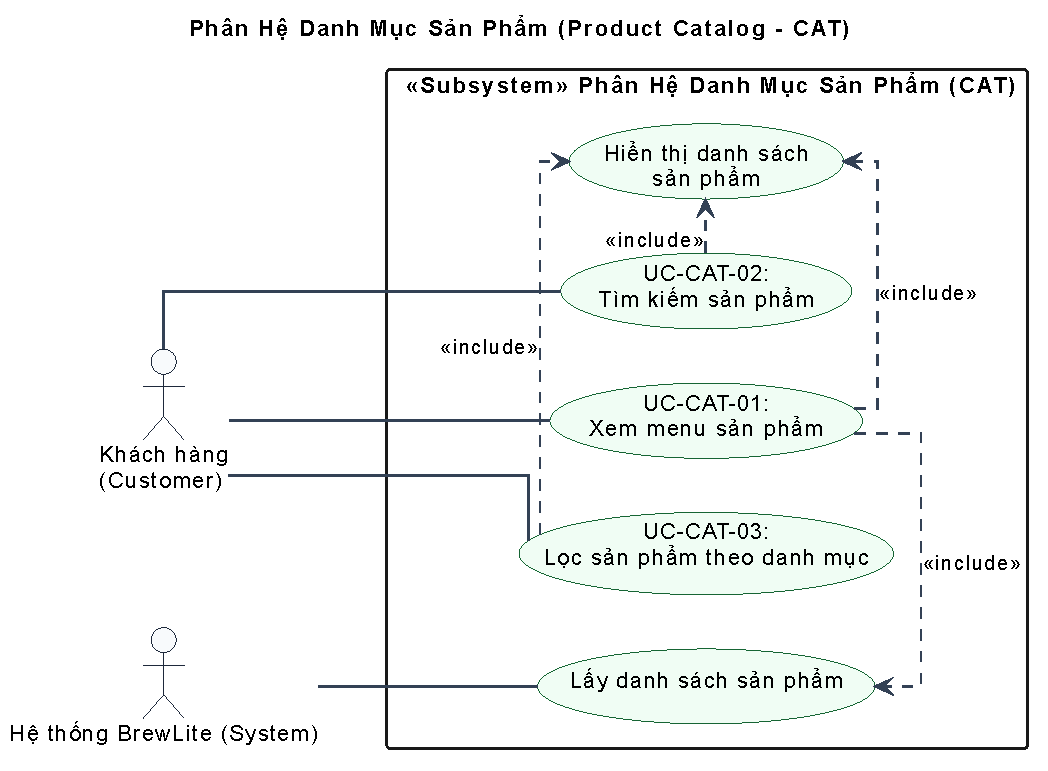
\includegraphics[width=0.75\textwidth]{figures/usecase-product-catalog.pdf}
    \caption{Sơ đồ Use Case - Phân hệ Danh mục Sản phẩm}
    \label{fig:usecase-product-catalog}
\end{figure}

\begin{table}[H]
\centering
\small
\caption{Đặc tả Use Case: Xem và Tìm kiếm Danh mục Sản phẩm (UC-CAT-01)}
\label{tab:uc-spec-catalog}
\begin{tabularx}{\textwidth}{p{2.8cm}X}
\toprule
\textbf{Mục} & \textbf{Chi tiết Đặc tả} \\
\midrule
\textbf{Actor} & Khách vãng lai, Khách hàng đăng nhập \\
\midrule
\textbf{Tiền điều kiện} & Hệ thống có dữ liệu sản phẩm và danh mục đã được kích hoạt trong CSDL. \\
\midrule
\textbf{Hậu điều kiện} & Danh sách sản phẩm tương ứng hiển thị trực quan trên giao diện thực đơn. \\
\midrule
\textbf{Luồng chính} & 
1. Người dùng truy cập trang Thực đơn (\texttt{/products}).\newline
2. Giao diện gửi request \texttt{GET /api/v1/categories} và \texttt{GET /api/v1/products}.\newline
3. Hệ thống trả về danh sách danh mục (Cà phê, Trà) và danh sách 10 sản phẩm (6 món cà phê, 4 món trà theo seed data).\newline
4. Khách hàng nhấp chọn tab phân loại (ví dụ "Cà phê") hoặc nhập từ khóa tìm kiếm (ví dụ "Latte").\newline
5. Hook \texttt{useProductCatalog} lọc lại danh sách hiển thị tương ứng kèm nhãn giá cơ bản và trạng thái còn hàng/hết hàng. \\
\midrule
\textbf{Luồng ngoại lệ} & 
- Lỗi kết nối mạng hoặc máy chủ backend: Hiển thị thông báo tải dữ liệu thất bại và cung cấp nút thử lại.\newline
- Không tìm thấy sản phẩm phù hợp: Hiển thị thông báo "Không tìm thấy sản phẩm nào phù hợp". \\
\bottomrule
\end{tabularx}
\end{table}

\clearpage
\subsection{Sơ đồ Hoạt động (Activity Diagram)}
Quy trình nạp và lọc danh mục sản phẩm được mô tả tại Hình~\ref{fig:activity-product-catalog}.

\begin{figure}[H]
    \centering
    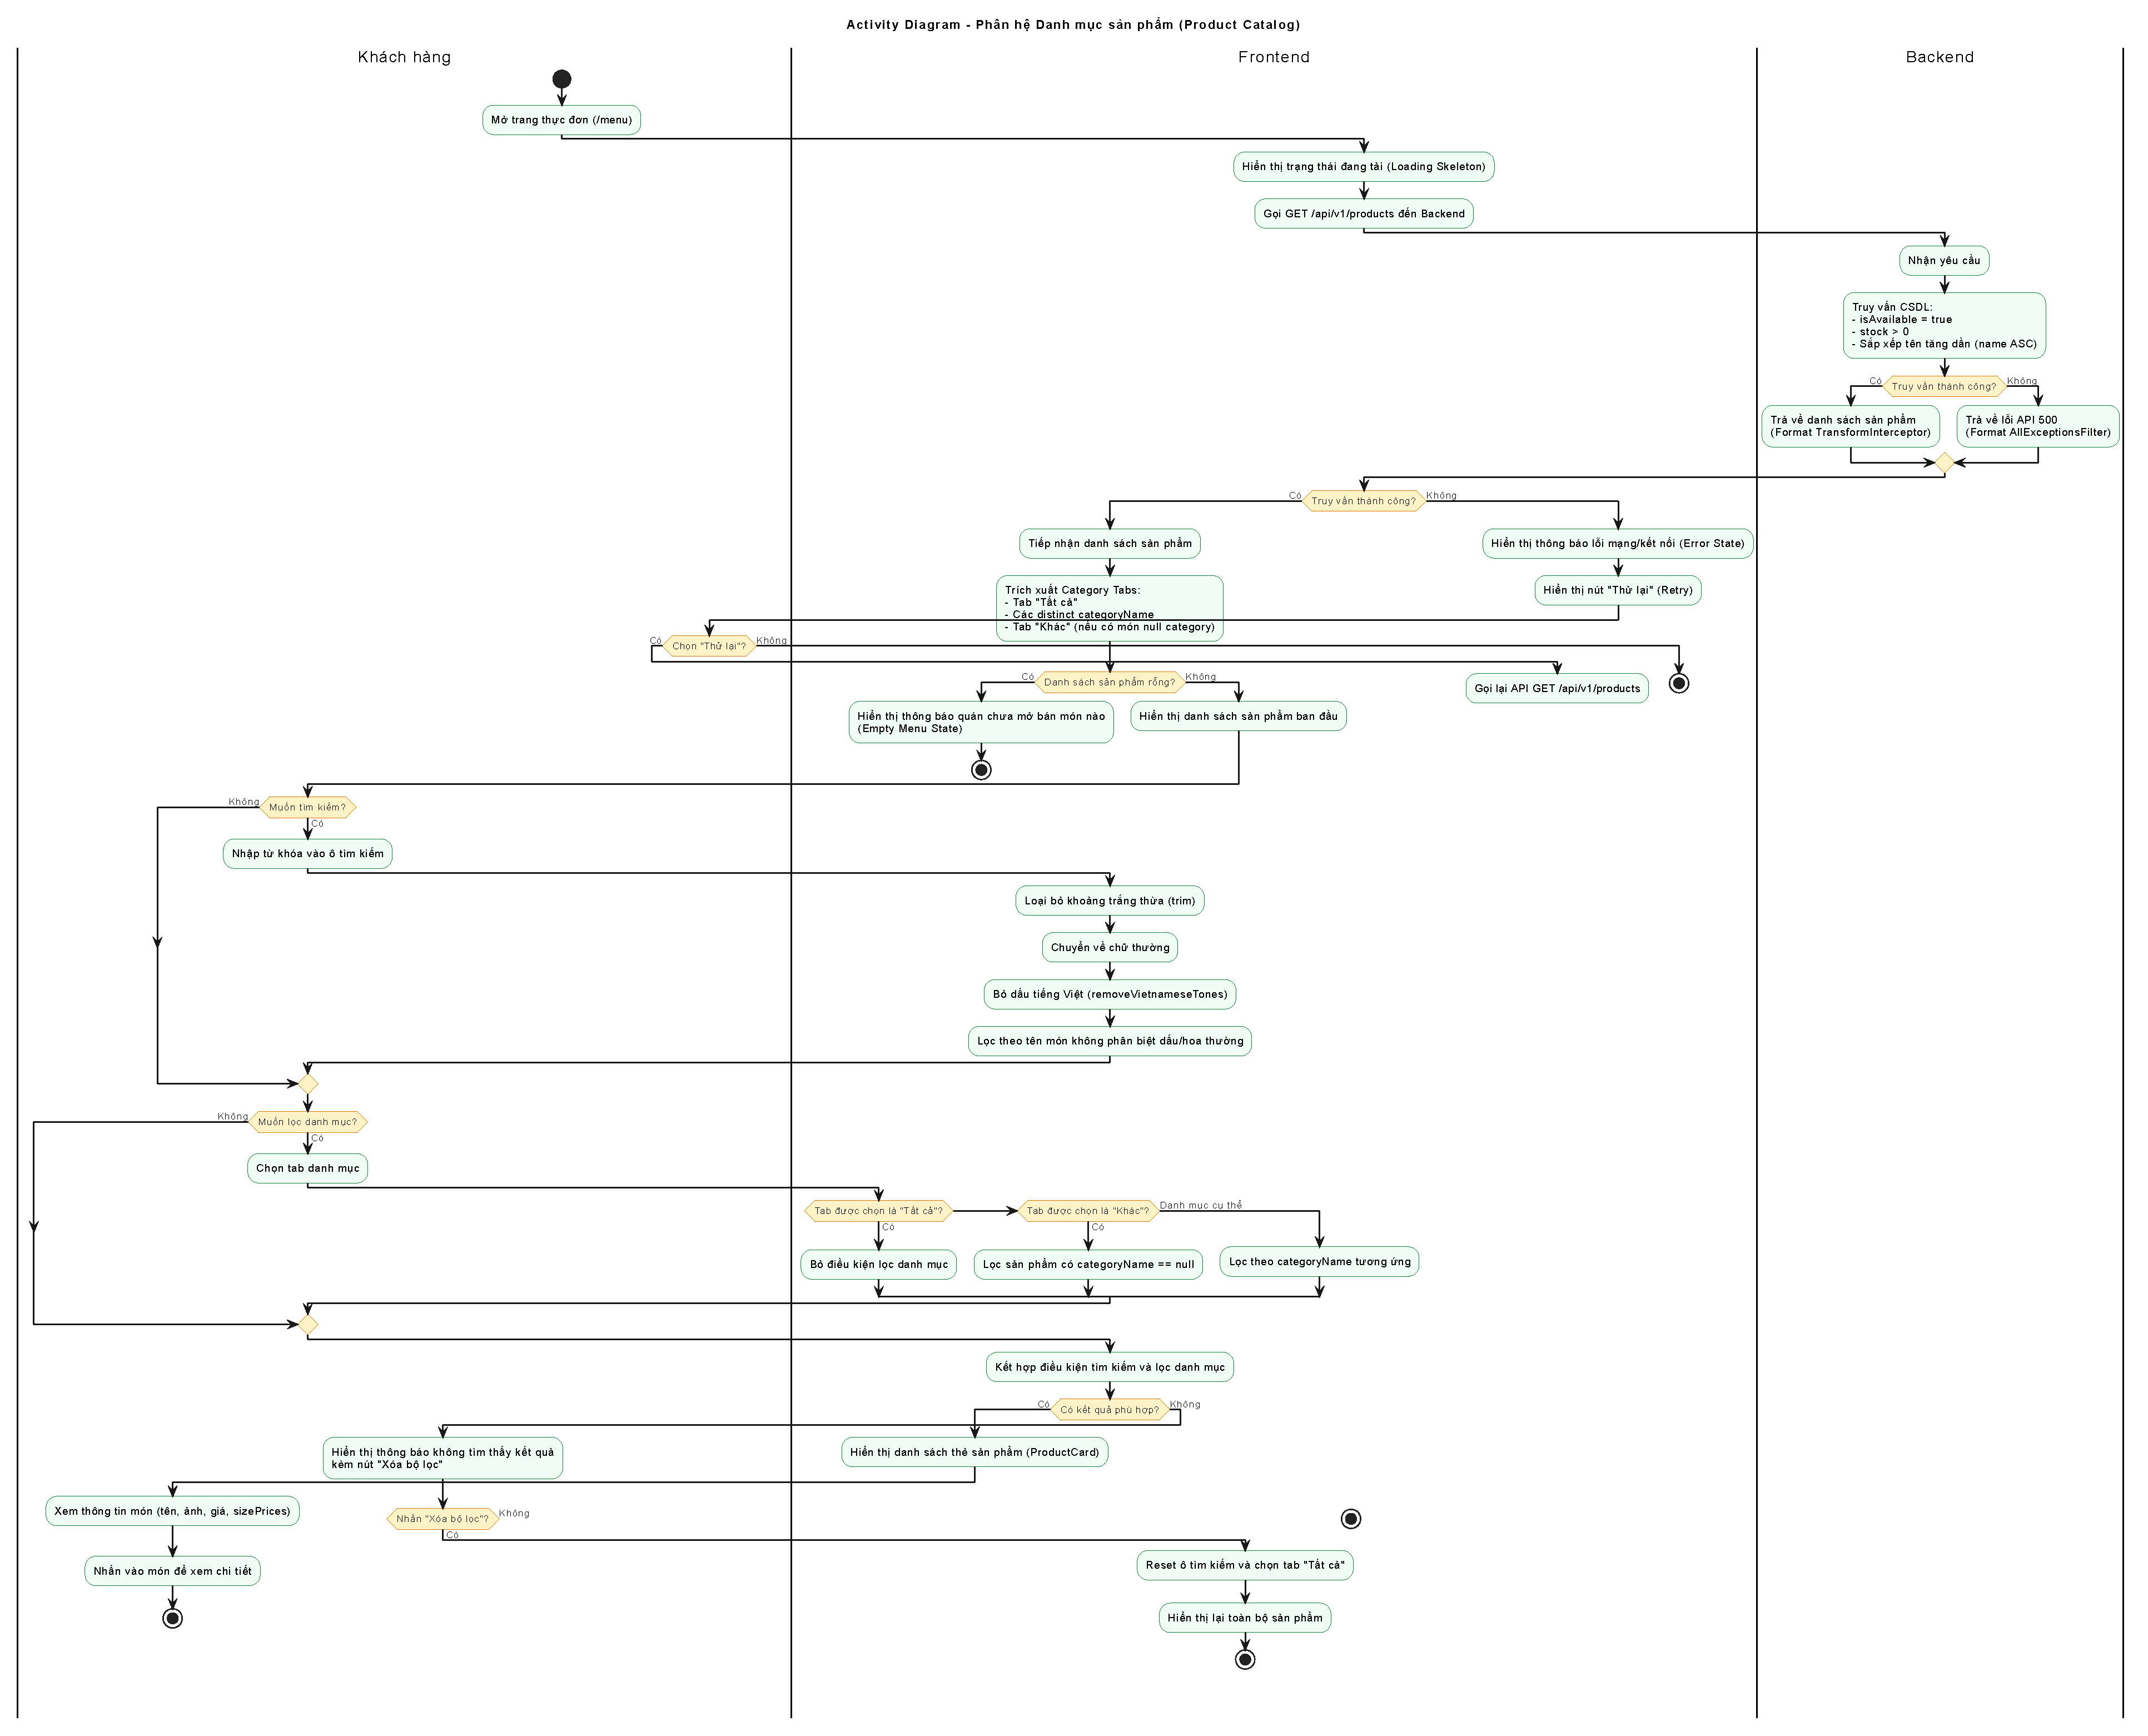
\includegraphics[width=\textwidth, height=0.98\textheight, keepaspectratio]{figures/activity-product-catalog.pdf}
    \caption{Sơ đồ Hoạt động - Phân hệ Danh mục Sản phẩm}
    \label{fig:activity-product-catalog}
\end{figure}

\clearpage
\subsection{Sơ đồ Tuần tự (Sequence Diagram)}
Sơ đồ Tuần tự phản ánh quá trình truy vấn danh mục và sản phẩm từ Frontend đến Backend Controller, Service và Prisma tại Hình~\ref{fig:sequence-product-catalog}.

\begin{figure}[H]
    \centering
    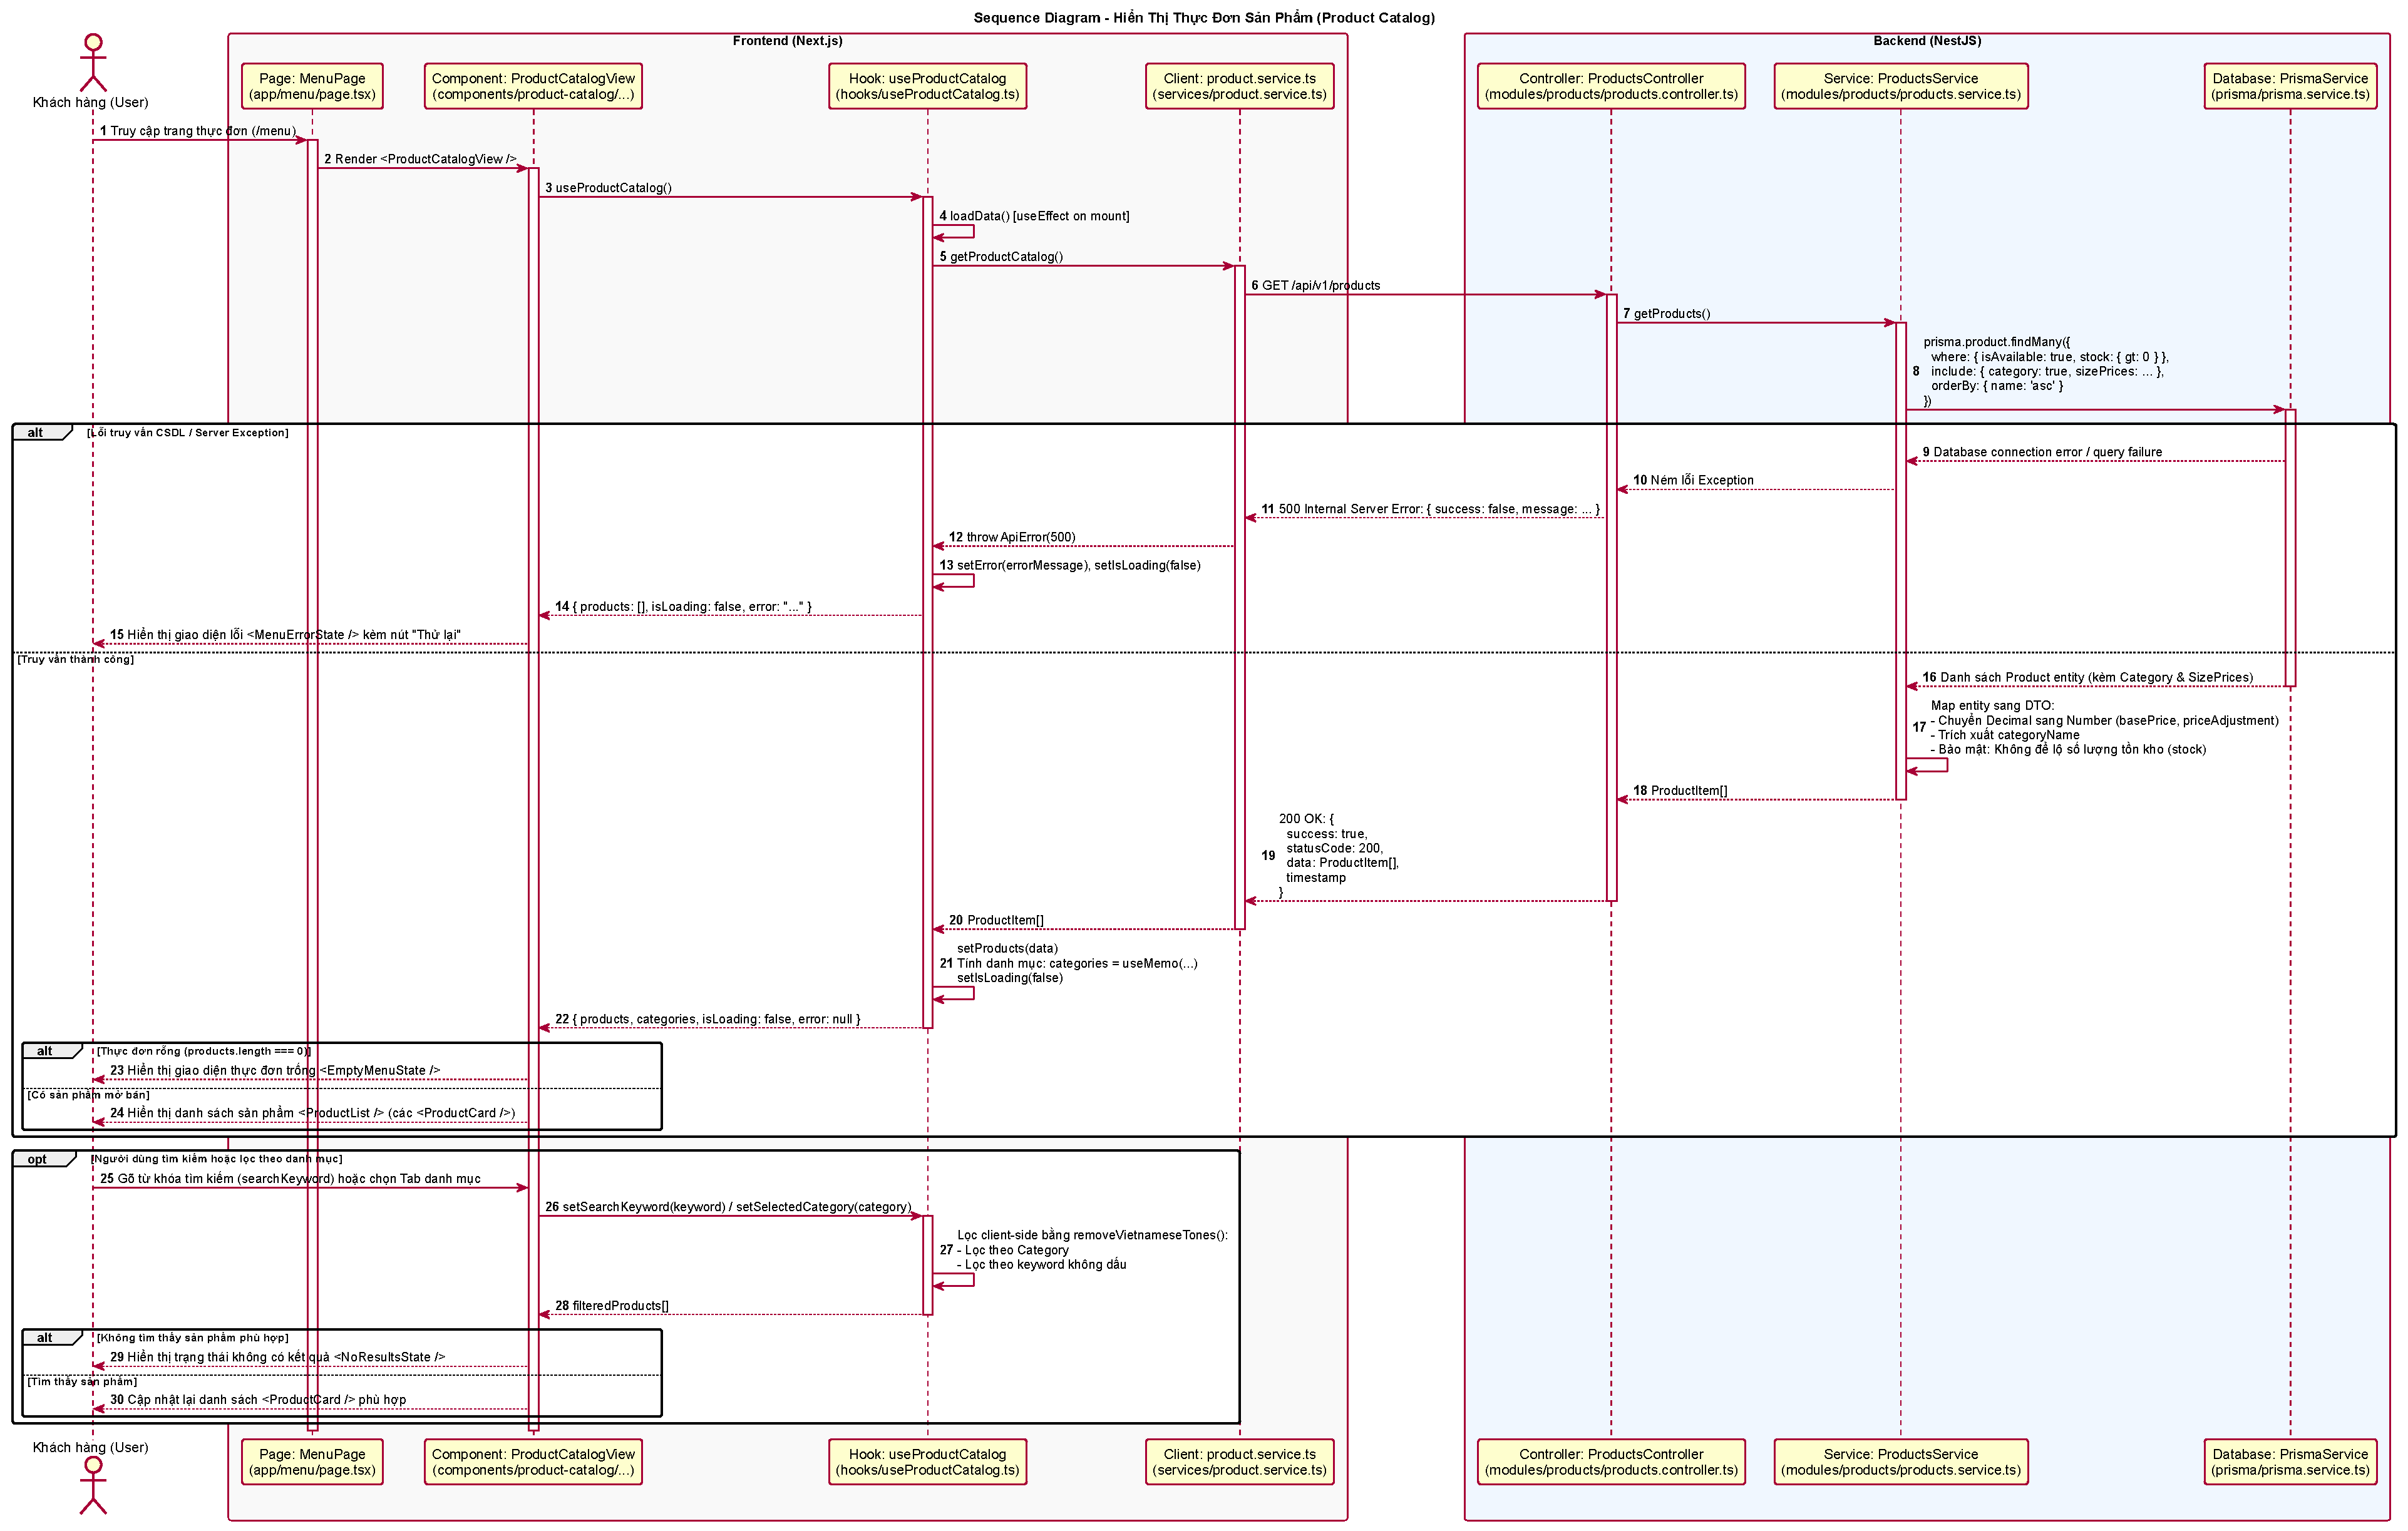
\includegraphics[width=\textwidth, height=0.80\textheight, keepaspectratio]{figures/sequence-product-catalog.pdf}
    \caption{Sơ đồ Tuần tự - Phân hệ Danh mục Sản phẩm}
    \label{fig:sequence-product-catalog}
\end{figure}

\clearpage
\subsection{Hợp đồng API (API Contract)}
\begin{table}[H]
\centering
\small
\caption{Danh mục API Endpoints - Phân hệ Danh mục Sản phẩm}
\label{tab:api-catalog}
\begin{tabularx}{\textwidth}{llp{4cm}X}
\toprule
\textbf{Phương thức} & \textbf{Endpoint} & \textbf{Tham số Query} & \textbf{Phản hồi chính} \\
\midrule
\texttt{GET} & \texttt{/api/v1/categories} & Không có & \texttt{200 OK}: Danh sách danh mục sắp xếp theo \texttt{displayOrder} tăng dần. \\
\texttt{GET} & \texttt{/api/v1/products} & \texttt{categoryId}, \texttt{search}, \texttt{availableOnly} & \texttt{200 OK}: Danh sách sản phẩm kèm thông tin giá cơ bản, hình ảnh và trạng thái khả dụng. \\
\bottomrule
\end{tabularx}
\end{table}

\subsection{Ánh xạ Cơ sở dữ liệu (Database Mapping)}
\begin{itemize}
    \item Truy vấn danh mục: \texttt{prisma.category.findMany(\{ orderBy: \{ displayOrder: 'asc' \} \})}.
    \item Truy vấn sản phẩm: \texttt{prisma.product.findMany(\{ where: \{ ...filter \}, include: \{ sizePrices: true, category: true \} \})}.
    \item Dữ liệu seed chuẩn gồm 2 danh mục chính ("Cà phê" - 6 món, "Trà" - 4 món), tổng cộng 10 sản phẩm mẫu được nạp vào bảng \texttt{categories} và \texttt{products}.
\end{itemize}

\subsection{Kịch bản Kiểm thử (Test Cases)}
\begin{table}[H]
\centering
\small
\caption{Tóm lược các Ca kiểm thử tiêu biểu - Phân hệ Danh mục}
\label{tab:tc-catalog}
\begin{tabularx}{\textwidth}{llp{2.6cm}p{3cm}Xc}
\toprule
\textbf{Mã TC} & \textbf{Loại} & \textbf{Tiền điều kiện} & \textbf{Endpoint / Màn hình} & \textbf{Kết quả mong đợi} & \textbf{Trạng thái} \\
\midrule
\texttt{TC-CAT-API-01} & Hợp lệ & DB có 2 danh mục & \texttt{GET /categories} & Trả về đủ 2 danh mục "Cà phê", "Trà" & Chưa chạy \\
\texttt{TC-CAT-API-02} & Hợp lệ & DB có 10 sản phẩm & \texttt{GET /products} & Trả về danh sách 10 món kèm \texttt{basePrice} & Chưa chạy \\
\texttt{TC-CAT-UI-01} & Giao diện & Trang \texttt{/products} & Thực đơn chính & Hiển thị tab "Tất cả", "Cà phê", "Trà" & Chưa chạy \\
\texttt{TC-CAT-UI-07} & Giao diện & Chọn tab "Cà phê" & Lọc danh mục & Hiển thị đúng 6 món cà phê từ seed data & Chưa chạy \\
\bottomrule
\end{tabularx}
\end{table}

\subsection{Giao diện Người dùng}
\begin{figure}[H]
    \centering
    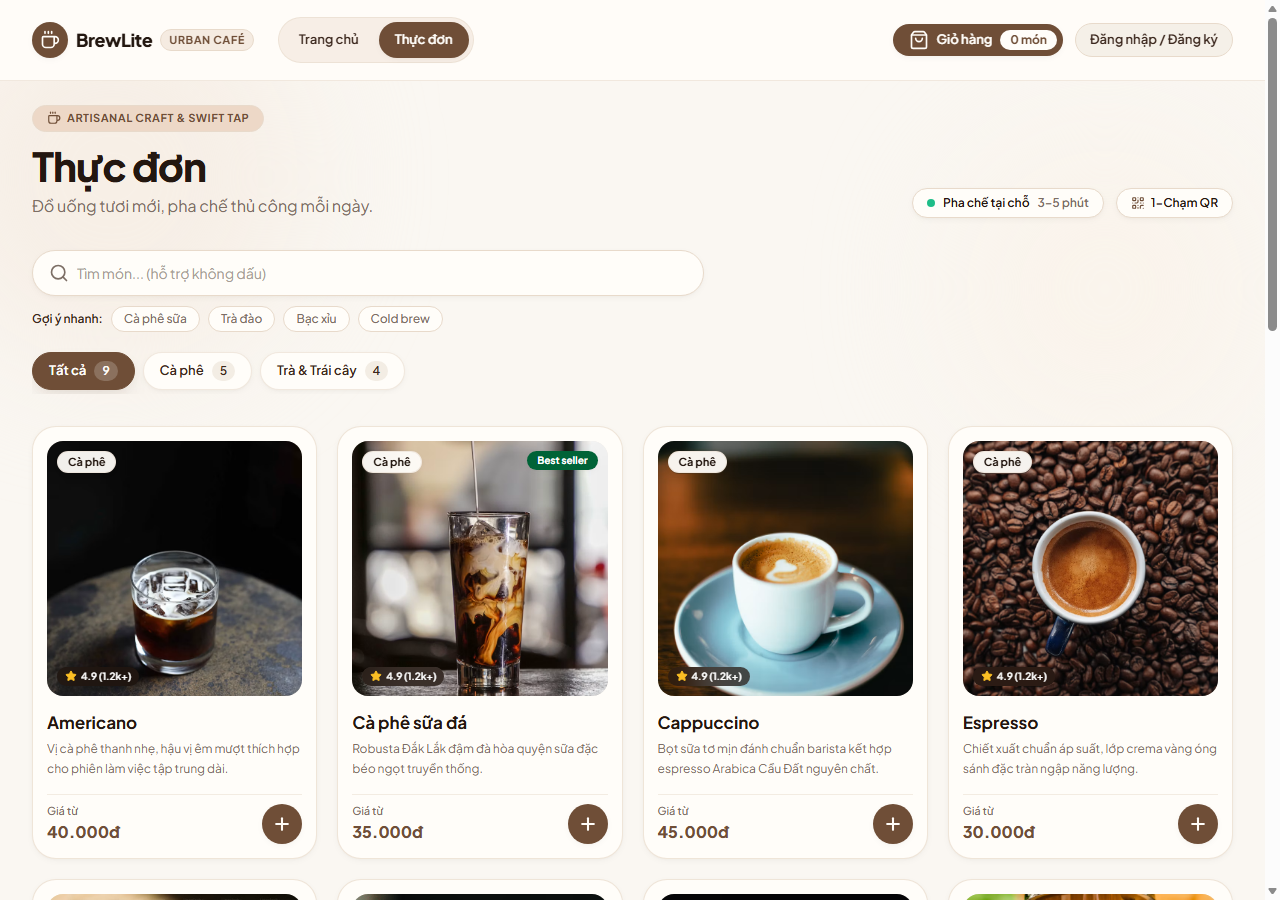
\includegraphics[width=0.92\textwidth]{figures/ui-catalog.png}
    \caption{Giao diện Thực đơn sản phẩm và Bộ lọc danh mục BrewLite}
    \label{fig:ui-catalog}
\end{figure}

\clearpage
\section{Phân hệ Chi tiết Sản phẩm (Product Detail)}

\subsection{Đặc tả Use Case}
Phân hệ Chi tiết Sản phẩm cung cấp thông tin toàn diện về đồ uống, bao gồm mô tả, thành phần dinh dưỡng/nguyên liệu và cho phép khách hàng cá nhân hóa món đồ uống theo sở thích cá nhân. Sơ đồ Use Case được minh họa tại Hình~\ref{fig:usecase-product-detail}.

\begin{figure}[H]
    \centering
    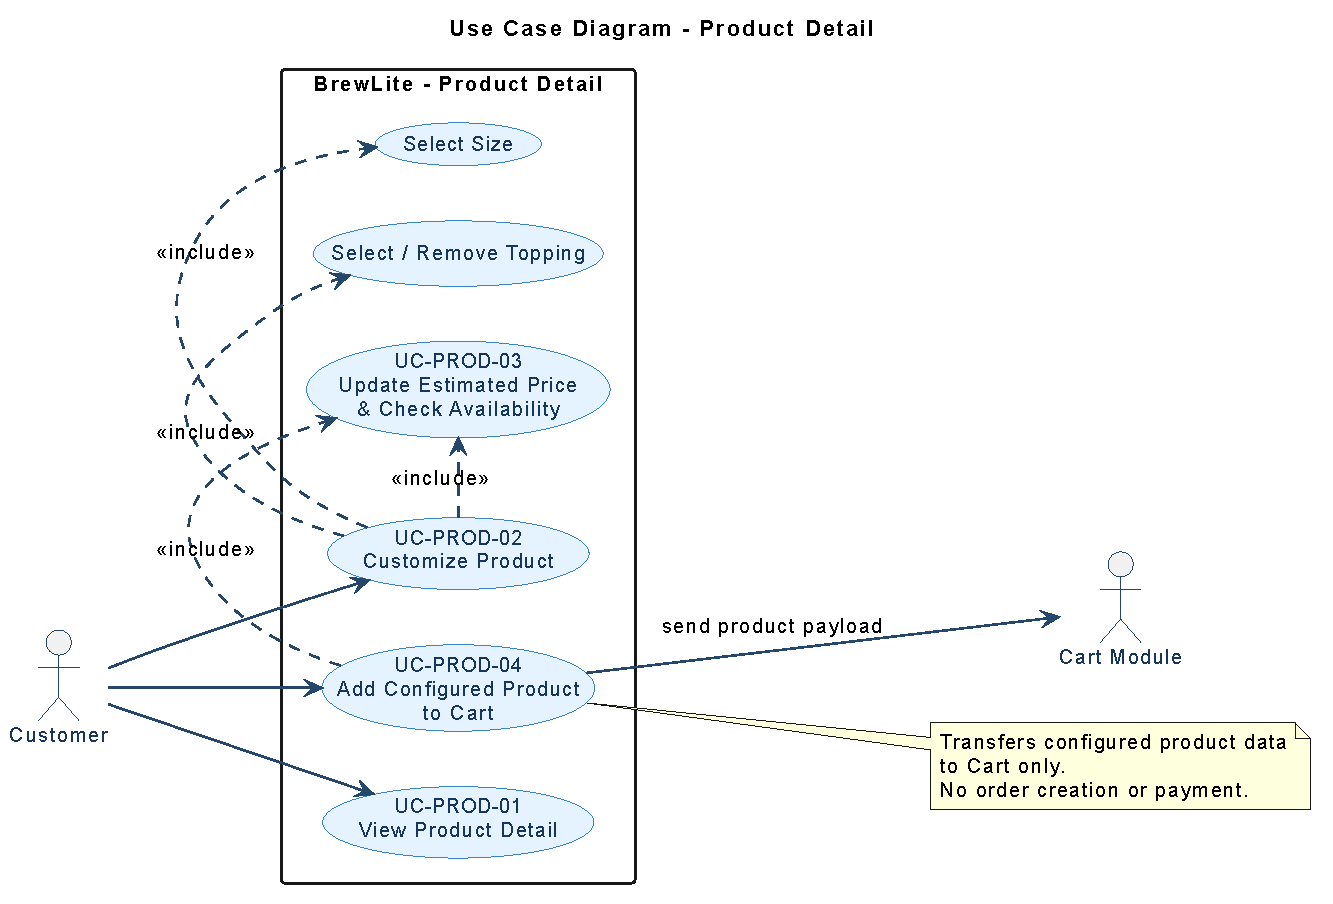
\includegraphics[width=0.75\textwidth]{figures/usecase-product-detail.pdf}
    \caption{Sơ đồ Use Case - Phân hệ Chi tiết Sản phẩm}
    \label{fig:usecase-product-detail}
\end{figure}

\begin{table}[H]
\centering
\small
\caption{Đặc tả Use Case: Xem chi tiết và Tùy biến món (UC-DET-01)}
\label{tab:uc-spec-detail}
\begin{tabularx}{\textwidth}{p{2.8cm}X}
\toprule
\textbf{Mục} & \textbf{Chi tiết Đặc tả} \\
\midrule
\textbf{Actor} & Khách vãng lai, Khách hàng đăng nhập \\
\midrule
\textbf{Tiền điều kiện} & Sản phẩm tồn tại trên hệ thống và có trạng thái \texttt{is\_available = true}. \\
\midrule
\textbf{Hậu điều kiện} & Thông tin món, các lựa chọn kích cỡ, mức ngọt, mức đá, danh sách topping và đơn giá tính toán động hiển thị đầy đủ trên màn hình. \\
\midrule
\textbf{Luồng chính} & 
1. Khách hàng nhấp vào thẻ món tại trang thực đơn.\newline
2. Trình duyệt điều hướng sang \texttt{/products/[id]}.\newline
3. Frontend gọi đồng thời \texttt{GET /api/v1/products/:id} và \texttt{GET /api/v1/toppings}.\newline
4. Giao diện hiển thị: tên món, hình ảnh, nút "Quay lại thực đơn", lựa chọn Size (Mặc định: M), mức đường (0\%, 30\%, 50\%, 70\%, 100\%), mức đá (0\%, 30\%, 50\%, 70\%, 100\%) và danh sách Topping kèm giá phụ thu.\newline
5. Khi người dùng thay đổi kích cỡ hoặc chọn thêm topping, giao diện tự động tính lại tổng đơn giá của món ăn theo thời gian thực.\newline
6. Khách hàng nhấn "Thêm vào giỏ hàng" để lưu món vào giỏ. \\
\midrule
\textbf{Luồng ngoại lệ} & 
- Sản phẩm không tồn tại: API trả về mã lỗi \texttt{404 Not Found}, giao diện hiển thị thông báo sản phẩm không tìm thấy và nút quay về thực đơn.\newline
- Sản phẩm hết hàng (\texttt{stock = 0}): Nút "Thêm vào giỏ hàng" bị vô hiệu hóa (\texttt{disabled}). \\
\bottomrule
\end{tabularx}
\end{table}

\clearpage
\subsection{Sơ đồ Hoạt động (Activity Diagram)}
Quy trình người dùng tương tác, chọn lựa tùy biến và kiểm tra trạng thái tồn kho được biểu diễn tại Hình~\ref{fig:activity-product-detail}.

\begin{figure}[H]
    \centering
    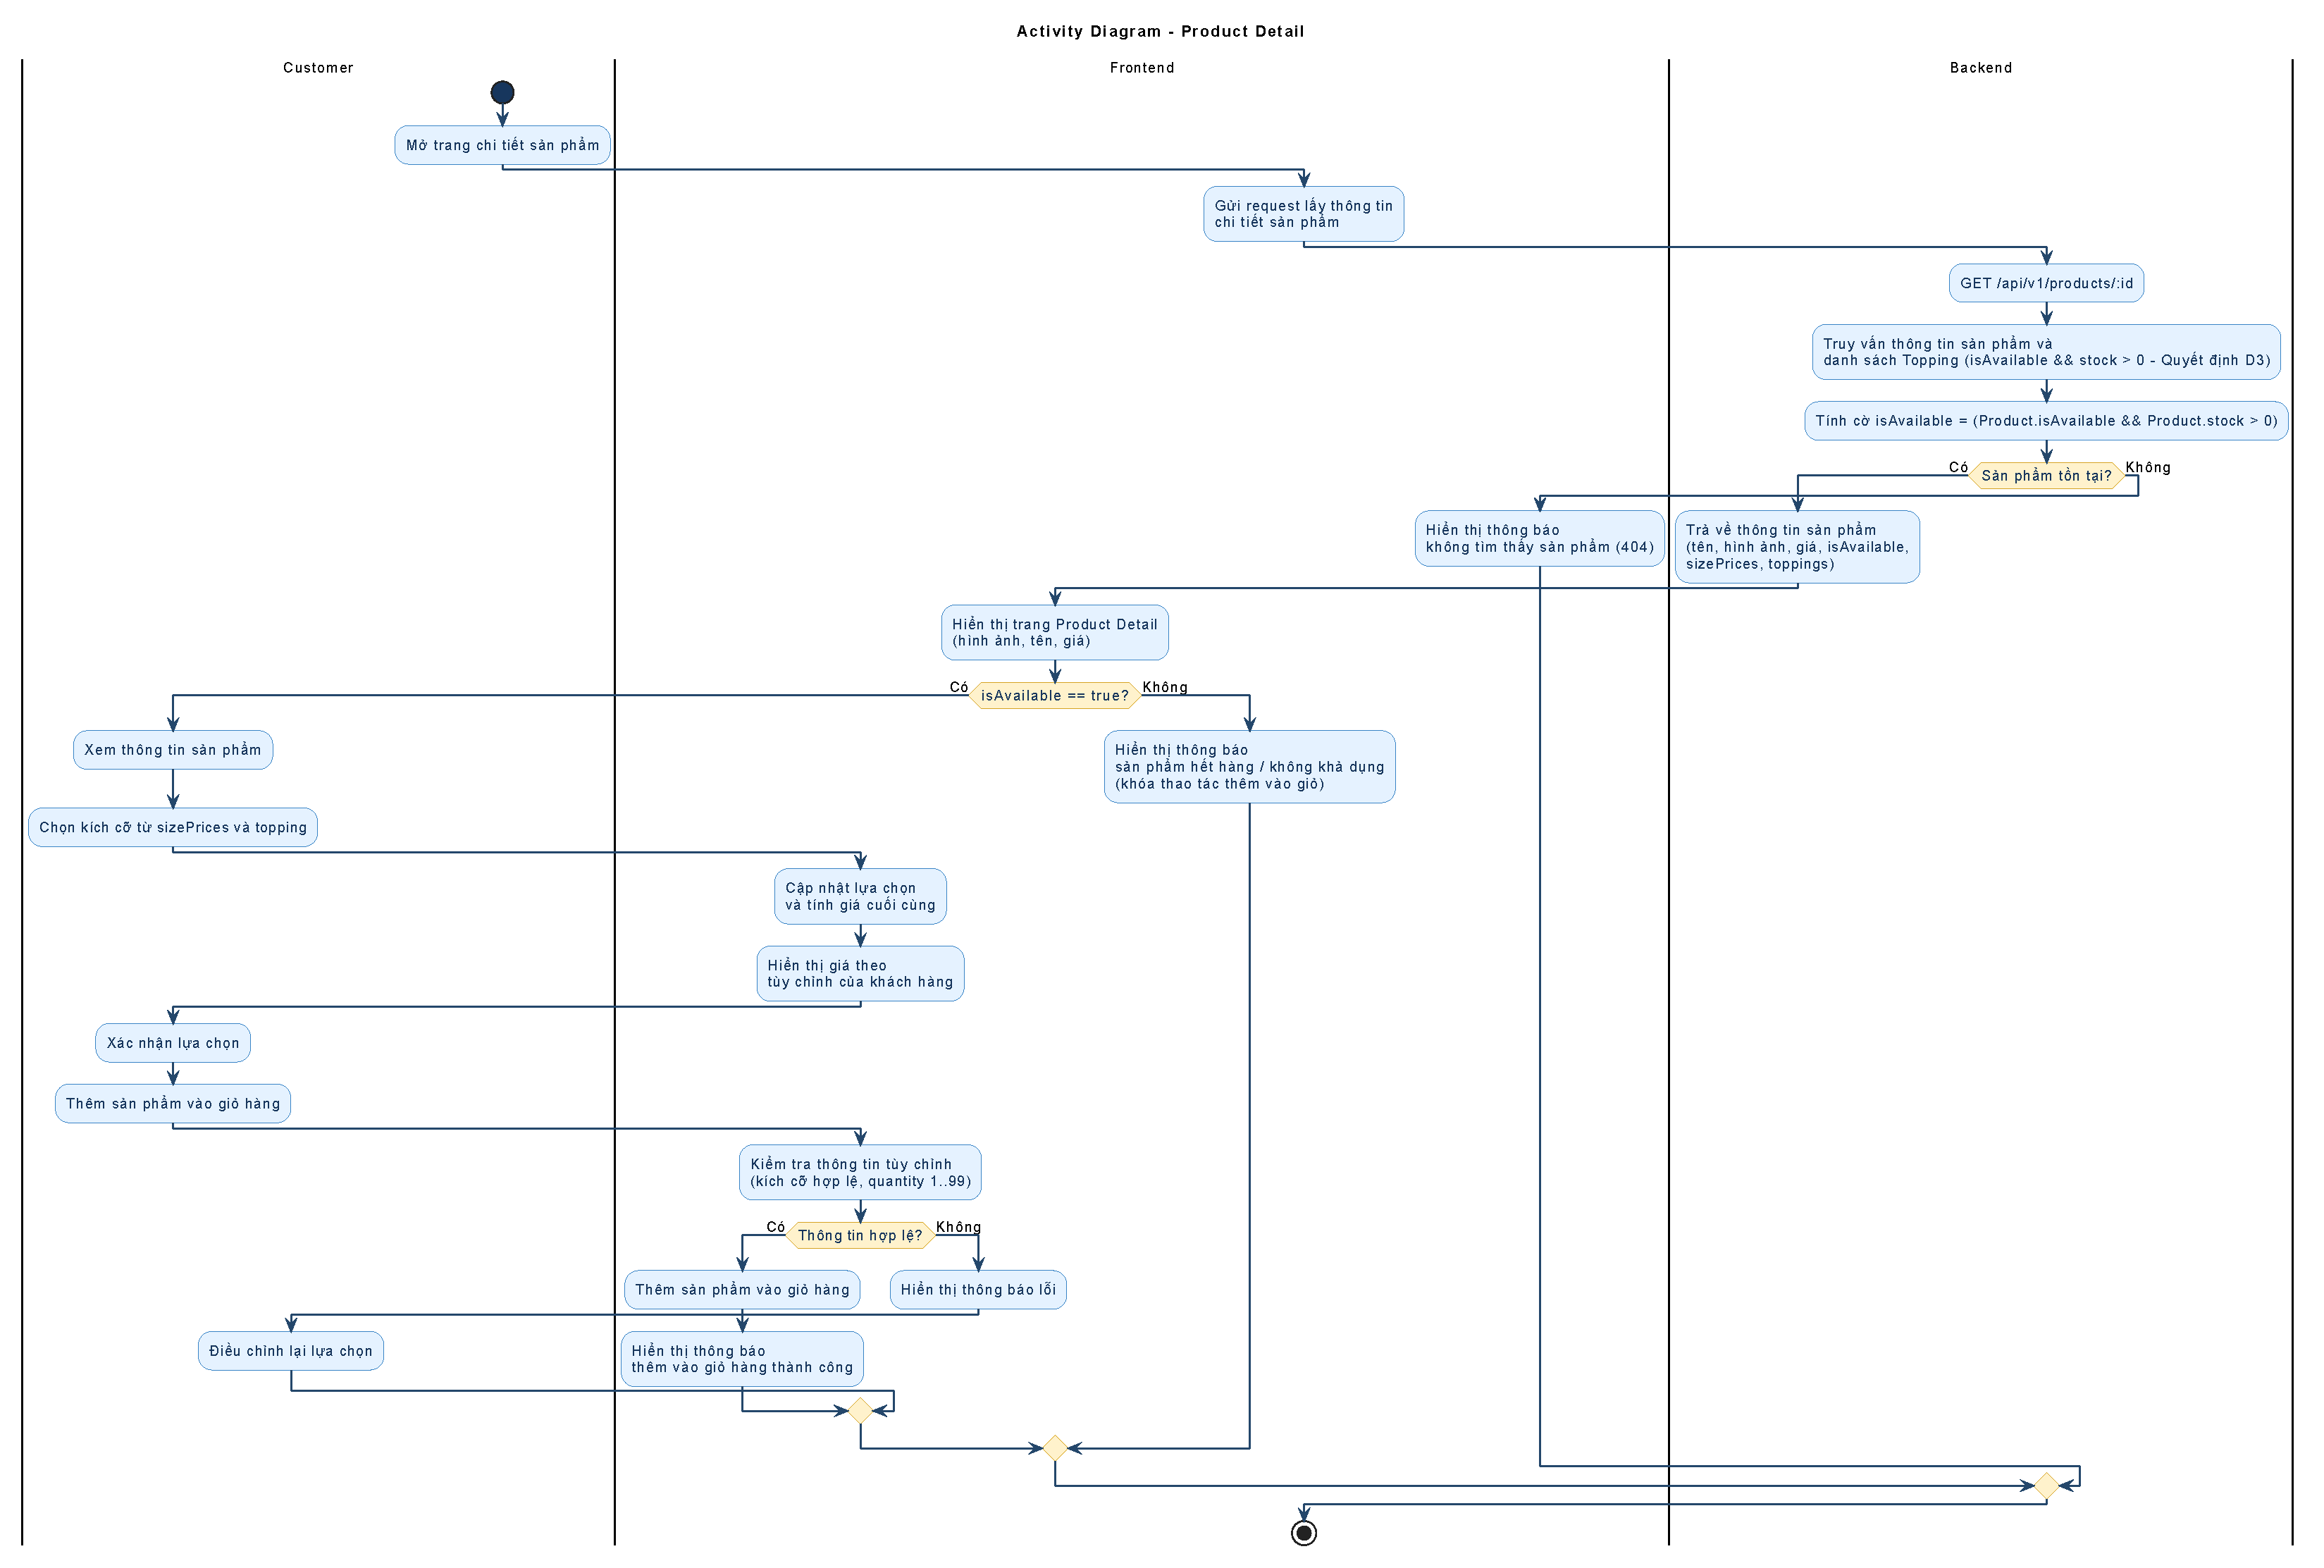
\includegraphics[width=\textwidth, height=0.80\textheight, keepaspectratio]{figures/activity-product-detail.pdf}
    \caption{Sơ đồ Hoạt động - Phân hệ Chi tiết Sản phẩm}
    \label{fig:activity-product-detail}
\end{figure}

\clearpage
\subsection{Sơ đồ Tuần tự (Sequence Diagram)}
Sơ đồ Tuần tự thể hiện các tương tác truy vấn dữ liệu chi tiết sản phẩm và danh mục topping tại Hình~\ref{fig:sequence-product-detail}.

\begin{figure}[H]
    \centering
    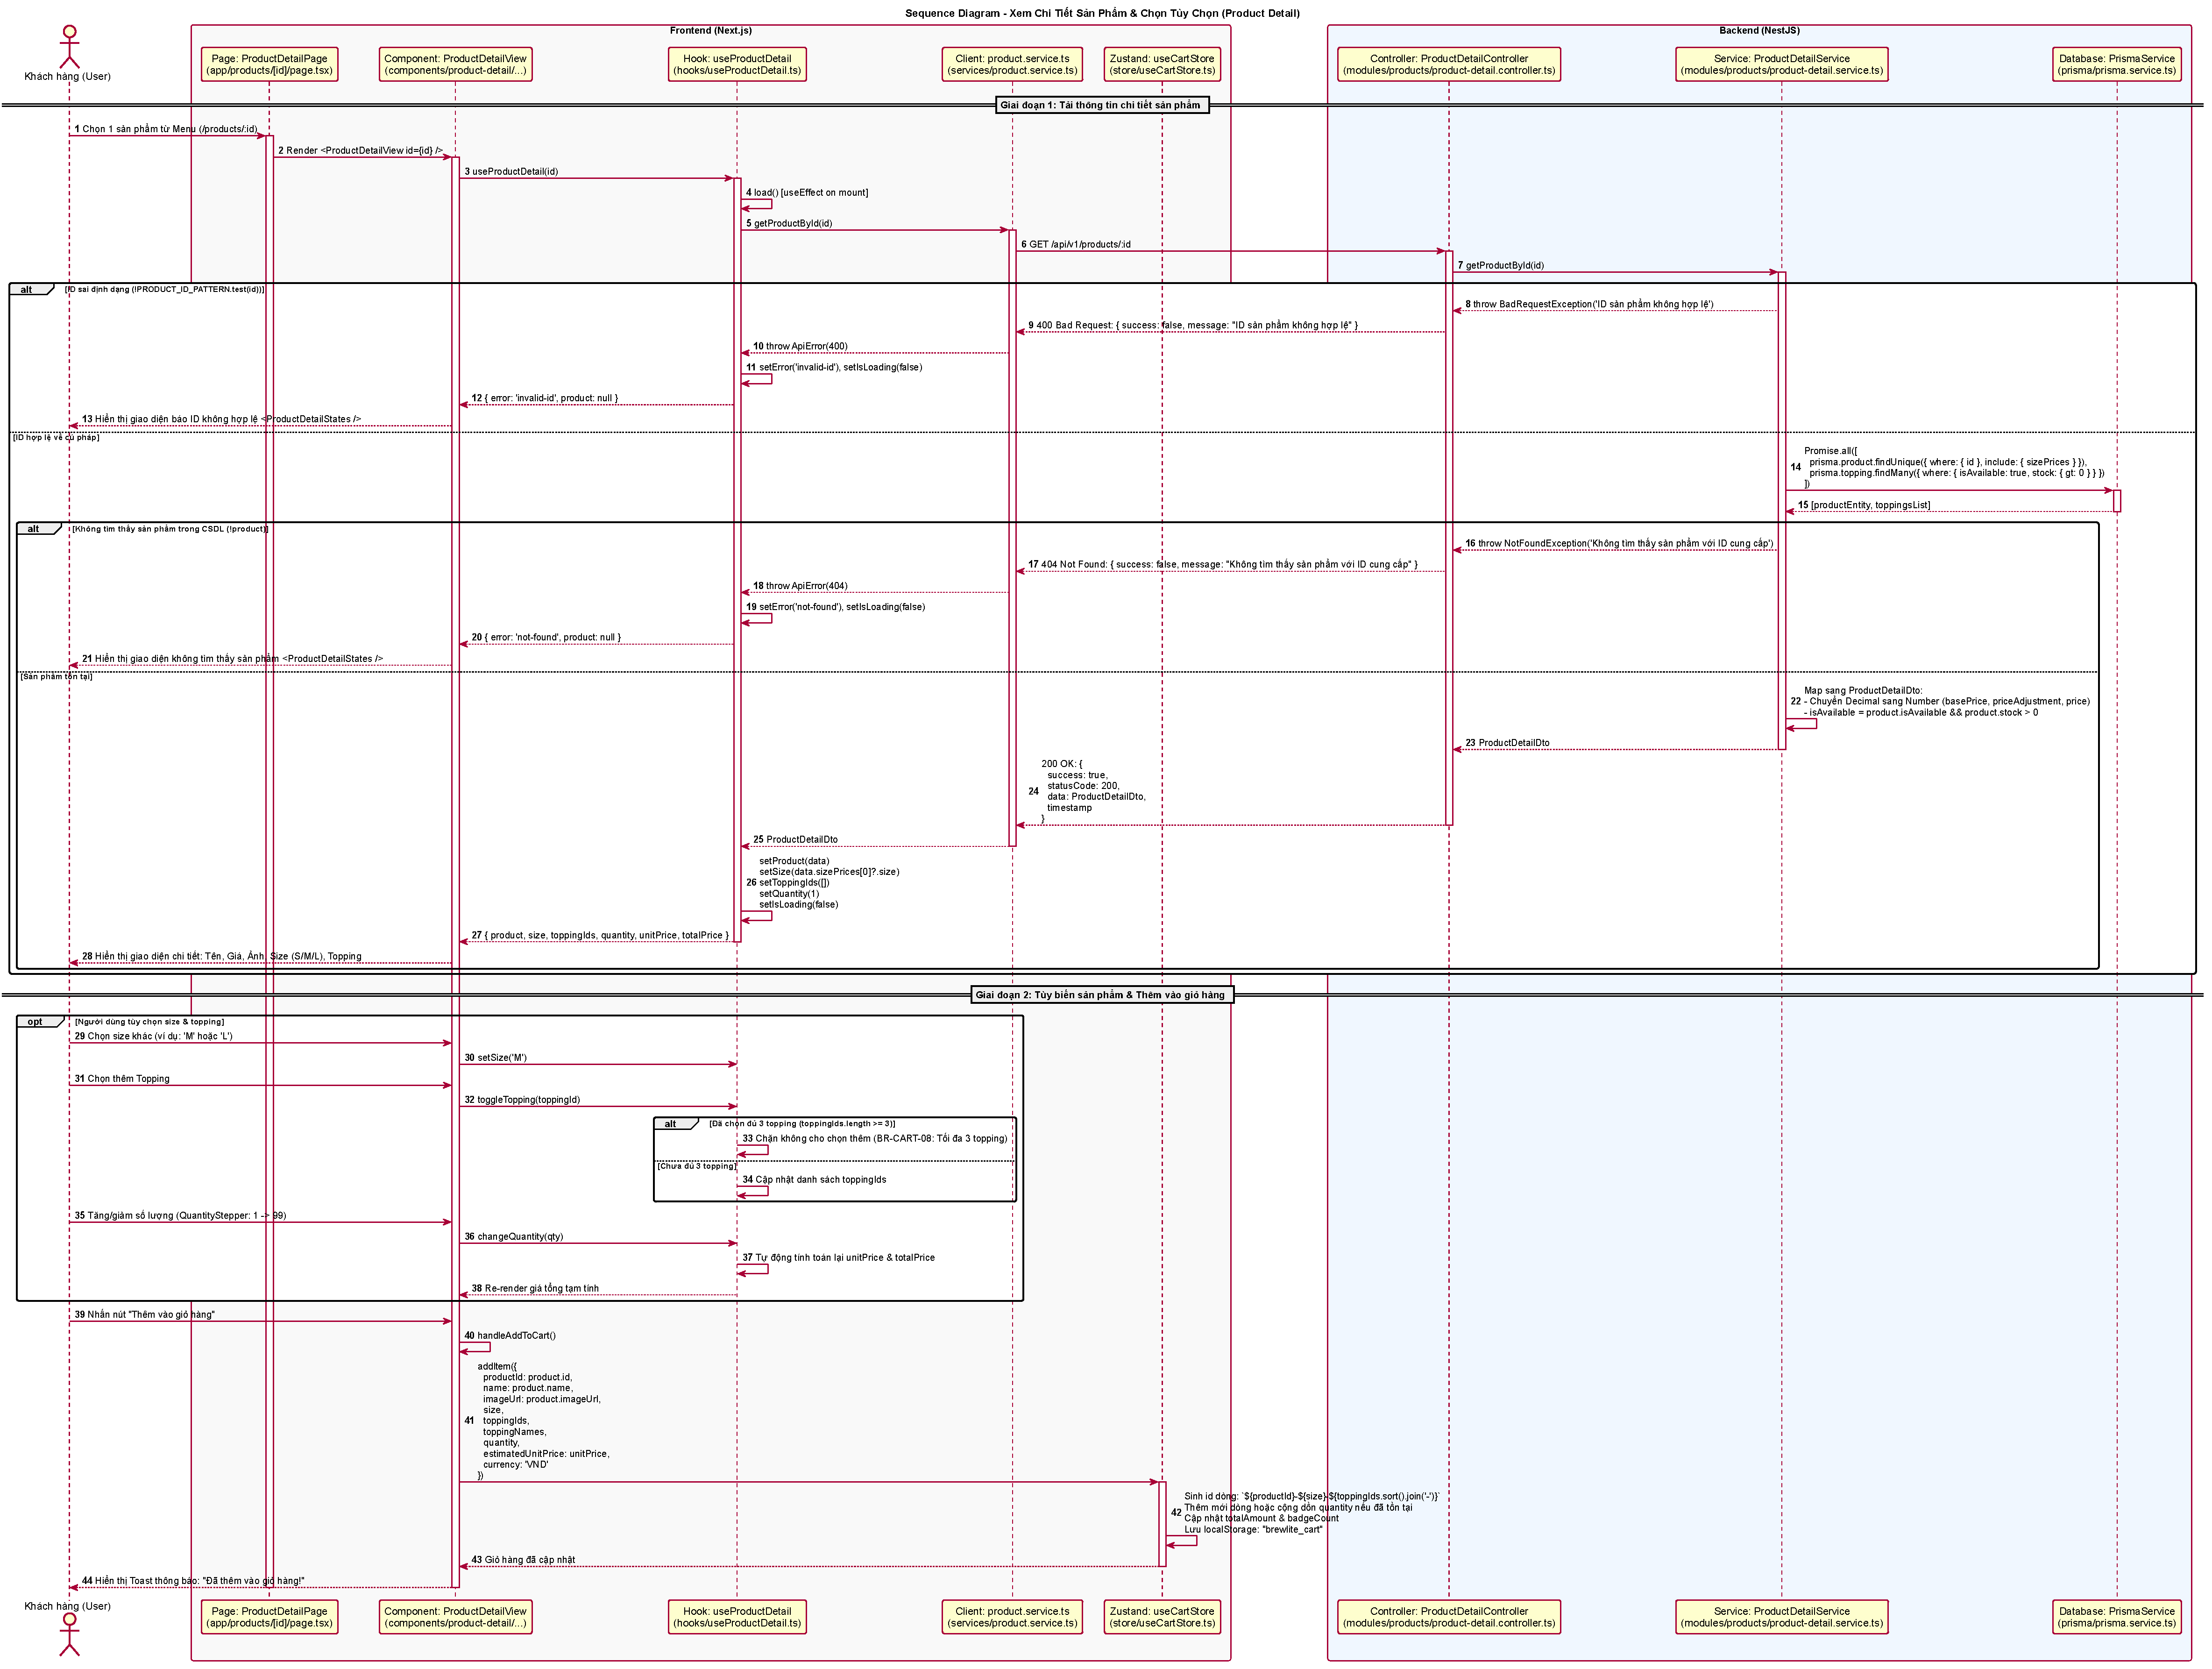
\includegraphics[width=\textwidth, height=0.80\textheight, keepaspectratio]{figures/sequence-product-detail.pdf}
    \caption{Sơ đồ Tuần tự - Phân hệ Chi tiết Sản phẩm}
    \label{fig:sequence-product-detail}
\end{figure}

\clearpage
\subsection{Hợp đồng API (API Contract)}
\begin{table}[H]
\centering
\small
\caption{Danh mục API Endpoints - Phân hệ Chi tiết Sản phẩm}
\label{tab:api-detail}
\begin{tabularx}{\textwidth}{llp{4cm}X}
\toprule
\textbf{Phương thức} & \textbf{Endpoint} & \textbf{Tham số Đường dẫn} & \textbf{Phản hồi chính} \\
\midrule
\texttt{GET} & \texttt{/api/v1/products/:id} & \texttt{id} (CUID của sản phẩm) & \texttt{200 OK}: Chi tiết sản phẩm kèm mảng \texttt{sizePrices} và thông tin \texttt{category}. Lỗi \texttt{404} nếu không tìm thấy. \\
\texttt{GET} & \texttt{/api/v1/toppings} & Không có & \texttt{200 OK}: Danh sách các loại topping đang hoạt động kèm giá và số lượng tồn. \\
\bottomrule
\end{tabularx}
\end{table}

\subsection{Ánh xạ Cơ sở dữ liệu (Database Mapping)}
\begin{itemize}
    \item Truy vấn chi tiết sản phẩm: \texttt{prisma.product.findUnique(\{ where: \{ id \}, include: \{ sizePrices: true, category: true \} \})}.
    \item Truy vấn danh sách topping: \texttt{prisma.topping.findMany(\{ where: \{ isAvailable: true \} \})}.
\end{itemize}

\subsection{Kịch bản Kiểm thử (Test Cases)}
\begin{table}[H]
\centering
\small
\caption{Tóm lược các Ca kiểm thử tiêu biểu - Phân hệ Chi tiết Sản phẩm}
\label{tab:tc-detail}
\begin{tabularx}{\textwidth}{llp{2.6cm}p{3cm}Xc}
\toprule
\textbf{Mã TC} & \textbf{Loại} & \textbf{Tiền điều kiện} & \textbf{Endpoint / Màn hình} & \textbf{Kết quả mong đợi} & \textbf{Trạng thái} \\
\midrule
\texttt{TC-DET-API-01} & Hợp lệ & ID sản phẩm tồn tại & \texttt{GET /products/:id} & HTTP 200, trả về đủ sizePrices (S, M, L) & Chưa chạy \\
\texttt{TC-DET-API-03} & Lỗi & ID không tồn tại & \texttt{GET /products/:id} & HTTP 404, message "Không tìm thấy sản phẩm" & Chưa chạy \\
\texttt{TC-DET-UI-01} & Giao diện & Mở trang chi tiết & Màn hình \texttt{/products/[id]} & Có nút "Quay lại thực đơn", nút "Thêm vào giỏ hàng" & Chưa chạy \\
\texttt{TC-DET-UI-04} & Giao diện & Chọn Size L (+10.000đ) & Tùy biến món & Đơn giá tự động cộng thêm phụ thu tương ứng & Chưa chạy \\
\bottomrule
\end{tabularx}
\end{table}

\subsection{Giao diện Người dùng}
\begin{figure}[H]
    \centering
    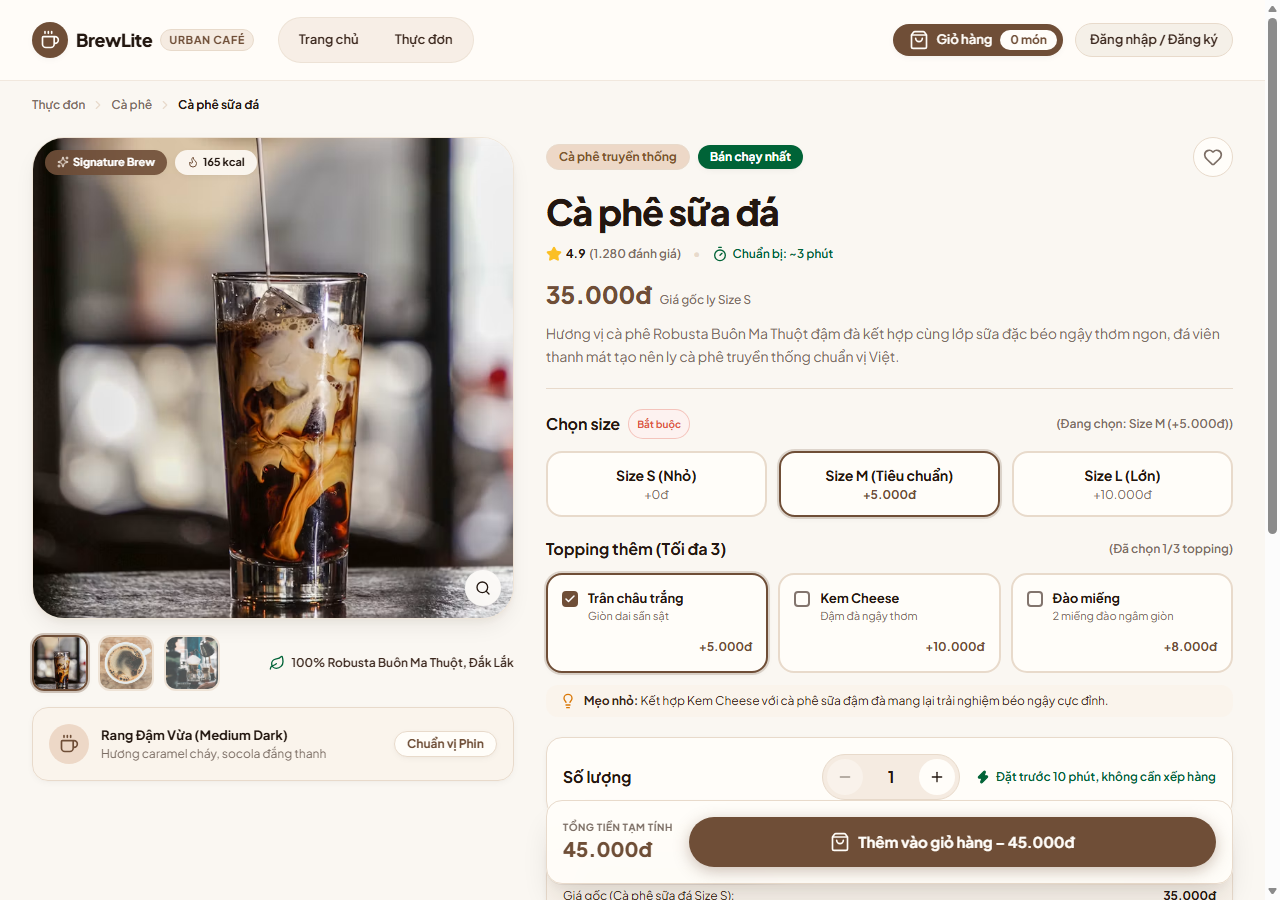
\includegraphics[width=0.92\textwidth]{figures/ui-detail.png}
    \caption{Giao diện Chi tiết món và Tùy biến Size / Topping}
    \label{fig:ui-detail}
\end{figure}

\clearpage
\section{Phân hệ Giỏ hàng (Cart)}

\subsection{Đặc tả Use Case}
Phân hệ Giỏ hàng quản lý danh sách các món đồ uống mà khách hàng đã lựa chọn kèm theo các tùy biến cụ thể trước khi tiến hành tạo đơn hàng chính thức. Để tối ưu hóa tài nguyên máy chủ và mang lại phản hồi tức thì cho người dùng, phân hệ này được thiết kế theo kiến trúc lưu trữ phía máy khách (\textit{Client-side State Management}). Sơ đồ Use Case được minh họa tại Hình~\ref{fig:usecase-cart}.

\begin{figure}[H]
    \centering
    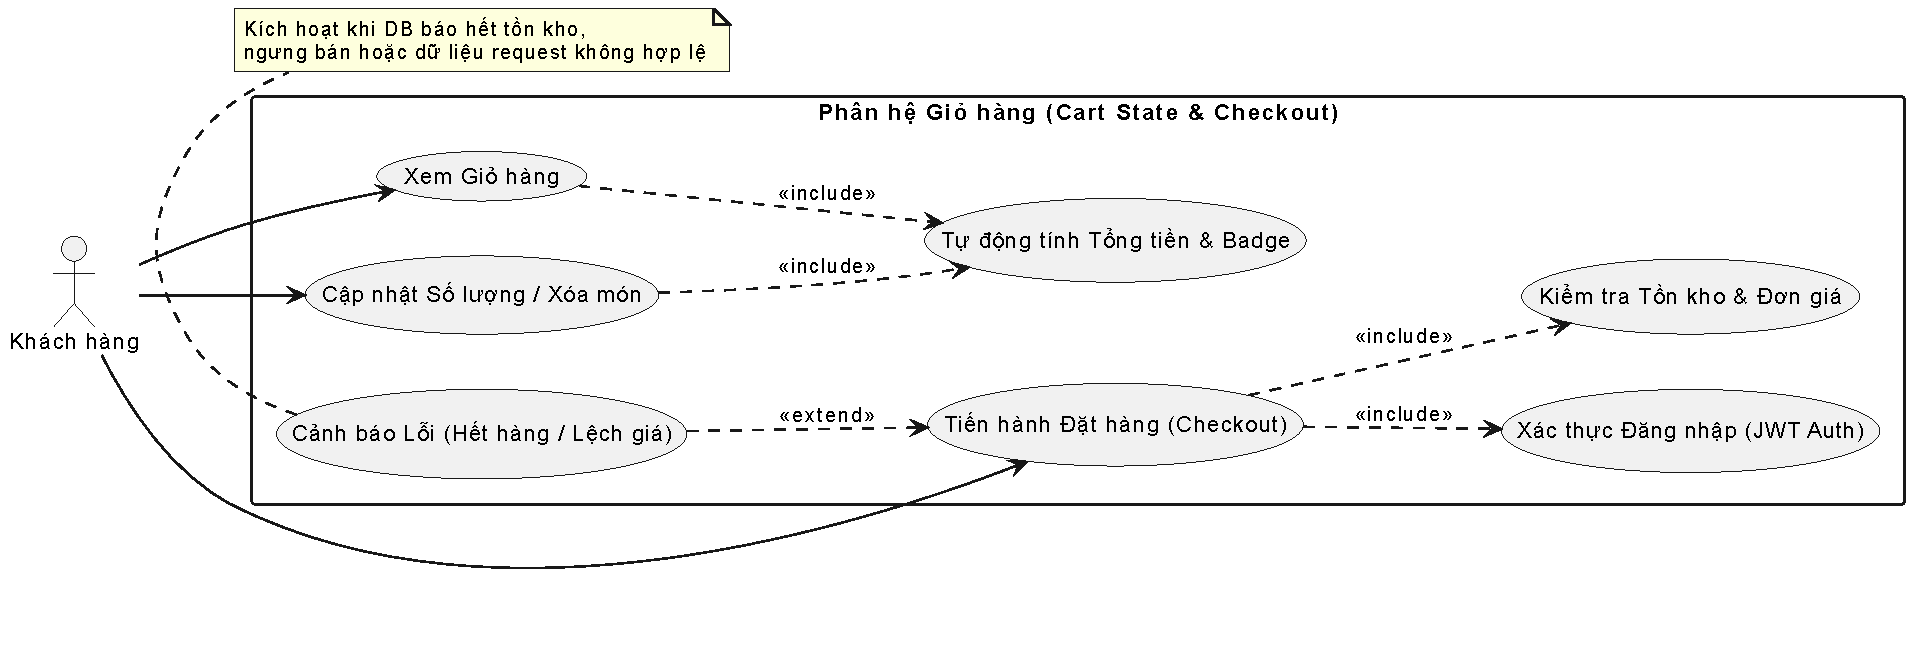
\includegraphics[width=0.75\textwidth]{figures/usecase-cart.pdf}
    \caption{Sơ đồ Use Case - Phân hệ Giỏ hàng}
    \label{fig:usecase-cart}
\end{figure}

\begin{table}[H]
\centering
\small
\caption{Đặc tả Use Case: Quản lý Giỏ hàng (UC-CART-01)}
\label{tab:uc-spec-cart}
\begin{tabularx}{\textwidth}{p{2.8cm}X}
\toprule
\textbf{Mục} & \textbf{Chi tiết Đặc tả} \\
\midrule
\textbf{Actor} & Khách vãng lai, Khách hàng đăng nhập \\
\midrule
\textbf{Tiền điều kiện} & Người dùng đã truy cập ứng dụng trên trình duyệt web. \\
\midrule
\textbf{Hậu điều kiện} & Danh sách món trong giỏ hàng, số lượng và tổng tiền tạm tính được cập nhật đồng bộ trong bộ nhớ máy khách (\texttt{localStorage} / Zustand state). \\
\midrule
\textbf{Luồng chính} & 
1. Người dùng thêm món từ trang chi tiết hoặc nhấn vào biểu tượng giỏ hàng tại thanh điều hướng (\texttt{Navbar}).\newline
2. Giao diện điều hướng sang trang \texttt{/cart}.\newline
3. Hệ thống nạp danh sách các món trong giỏ từ bộ nhớ cục bộ.\newline
4. Người dùng có thể tăng/giảm số lượng từng món, xóa từng món hoặc xóa toàn bộ giỏ.\newline
5. Bộ tính giá phía client tự động tính toán lại mục "Tạm tính" cho từng dòng và tổng giá trị đơn hàng.\newline
6. Khi người dùng nhấn "Thanh toán" (hoặc "Tiến hành đặt hàng"), hệ thống kiểm tra điều kiện đăng nhập trước khi chuyển sang bước đặt hàng. \\
\midrule
\textbf{Luồng ngoại lệ} & 
- Giỏ hàng không có sản phẩm nào: Giao diện hiển thị thông báo "Giỏ hàng của bạn đang trống" và nút điều hướng "Xem thực đơn". \\
\bottomrule
\end{tabularx}
\end{table}

\clearpage
\subsection{Sơ đồ Hoạt động (Activity Diagram)}
Quy trình quản lý thêm, sửa, xóa và tính toán giá trị giỏ hàng được thể hiện tại Hình~\ref{fig:activity-cart}.

\begin{figure}[H]
    \centering
    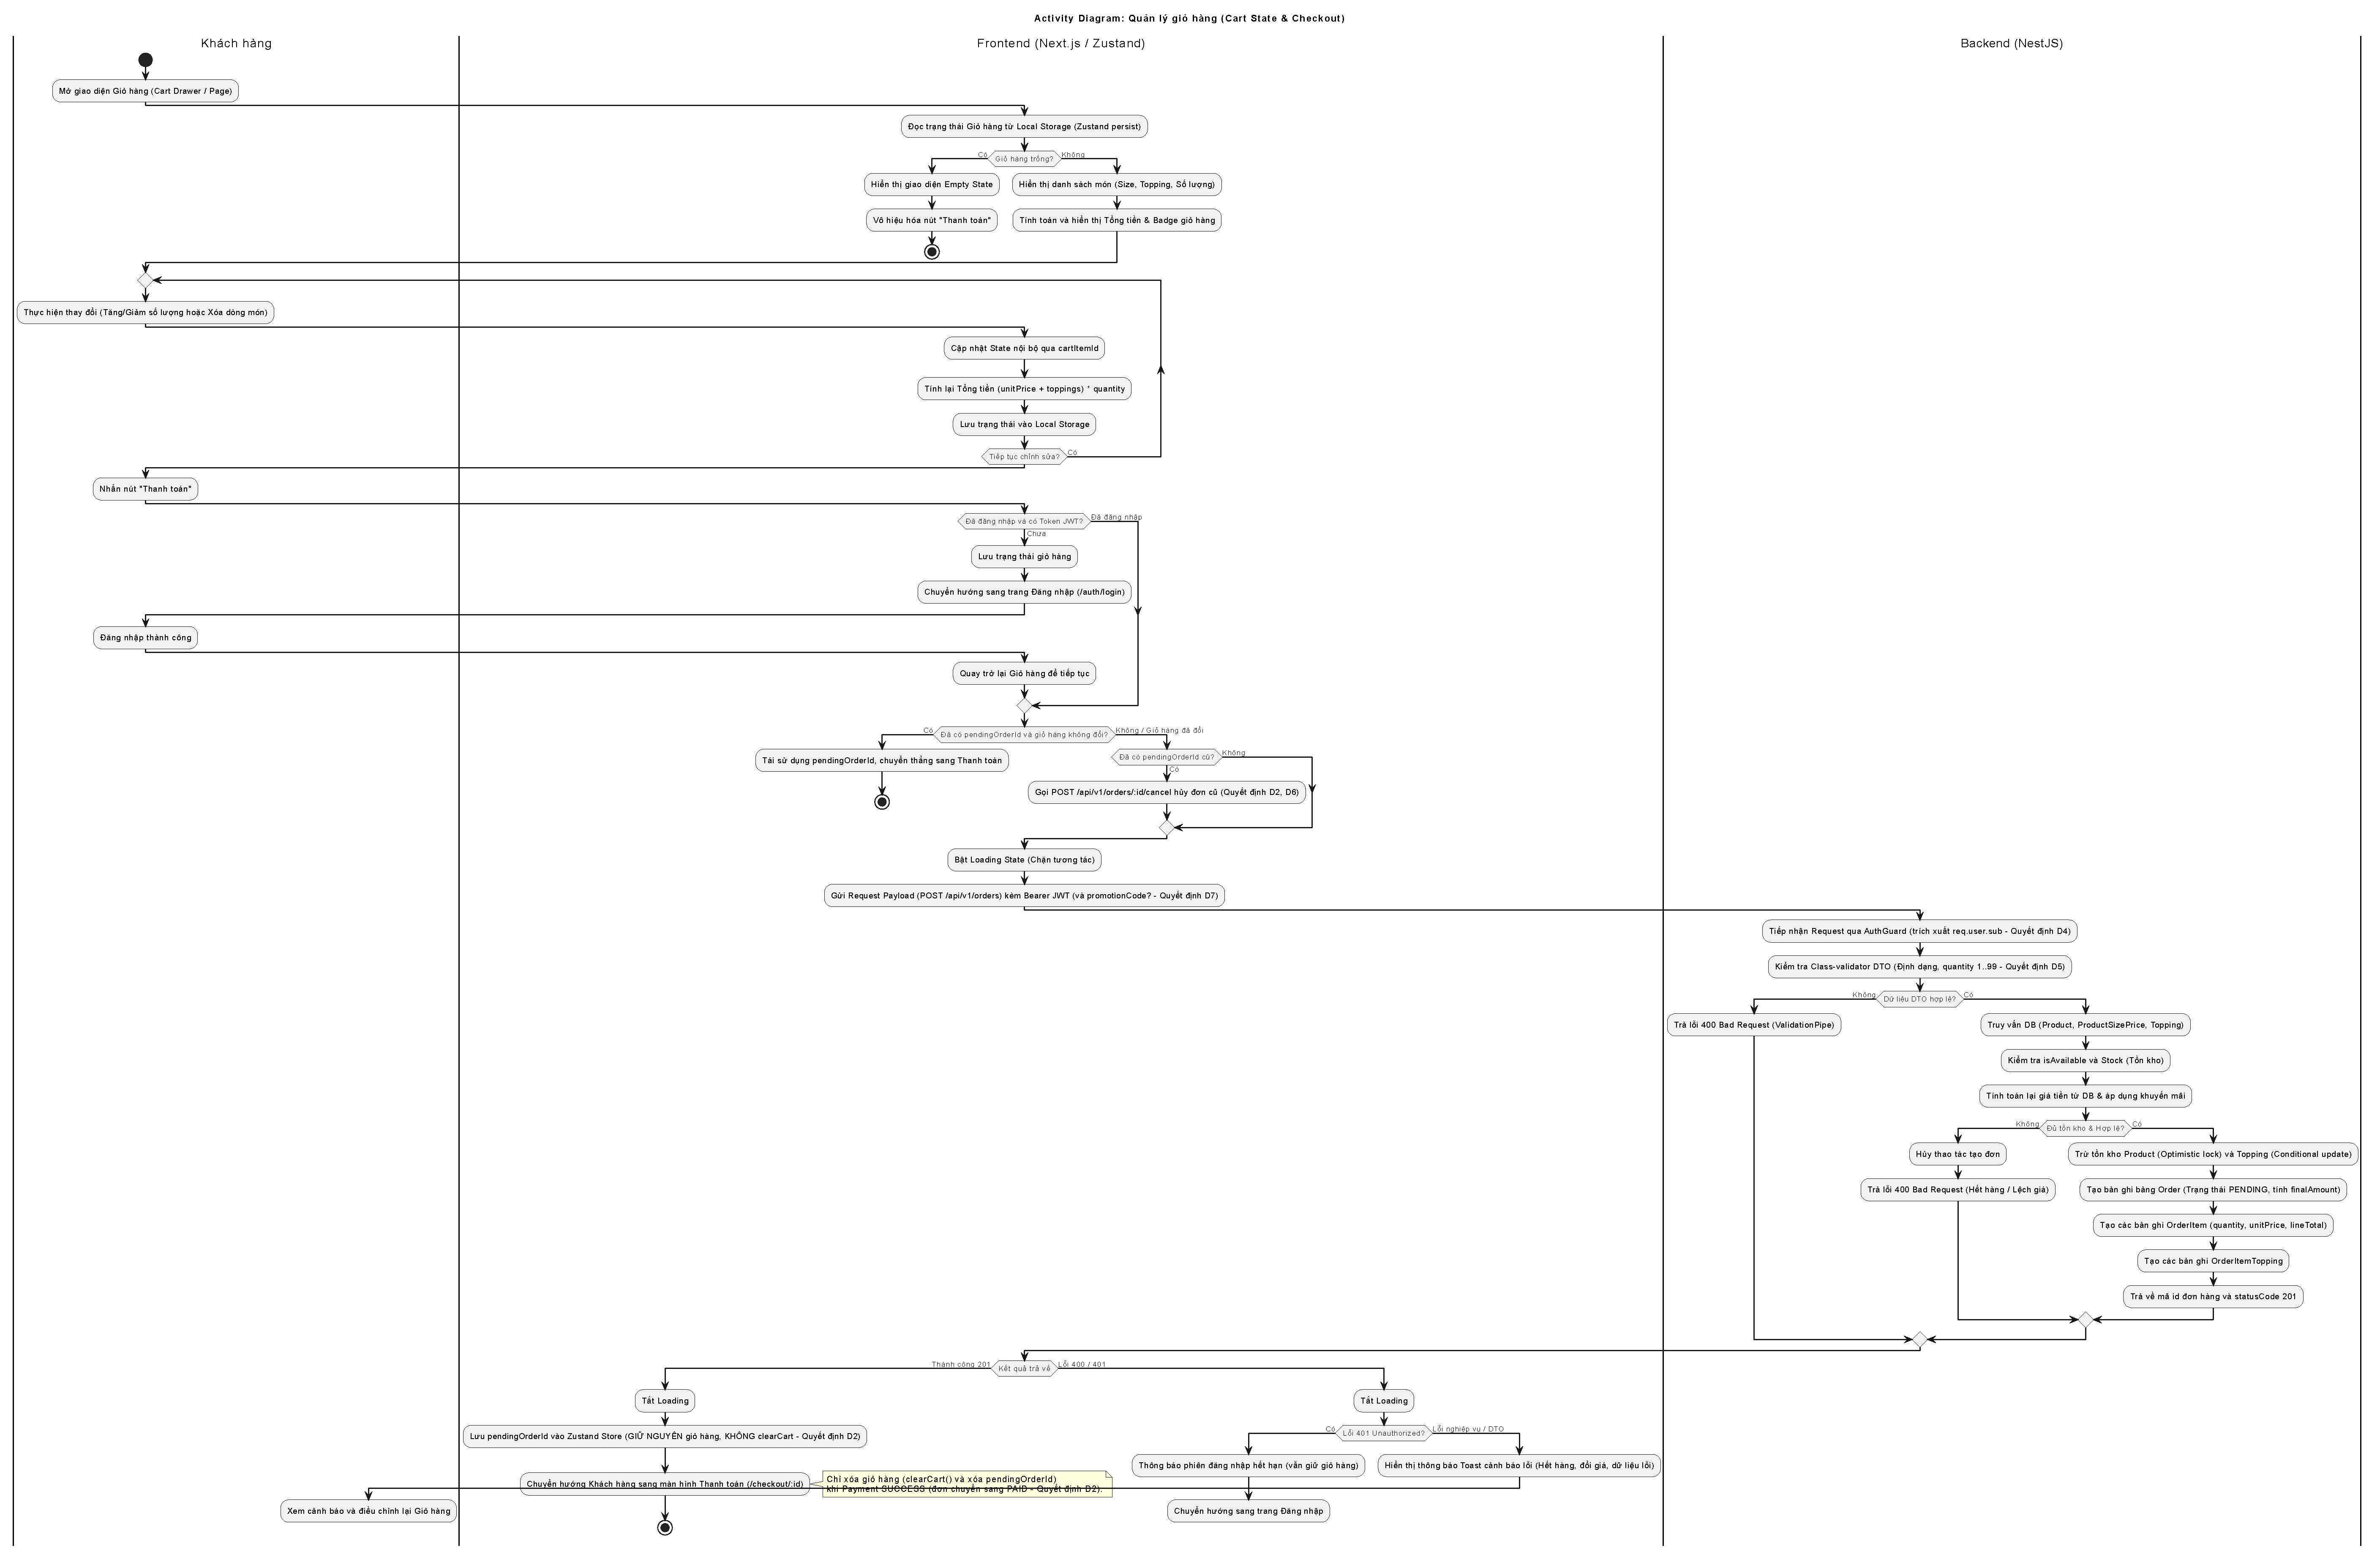
\includegraphics[width=\textwidth, height=0.80\textheight, keepaspectratio]{figures/activity-cart.pdf}
    \caption{Sơ đồ Hoạt động - Phân hệ Giỏ hàng}
    \label{fig:activity-cart}
\end{figure}

\clearpage
\subsection{Sơ đồ Tuần tự (Sequence Diagram)}
Sơ đồ Tuần tự minh họa luồng xử lý hoàn toàn khép kín ở phía Frontend giữa giao diện, Store quản lý trạng thái và LocalStorage tại Hình~\ref{fig:sequence-cart}.

\begin{figure}[H]
    \centering
    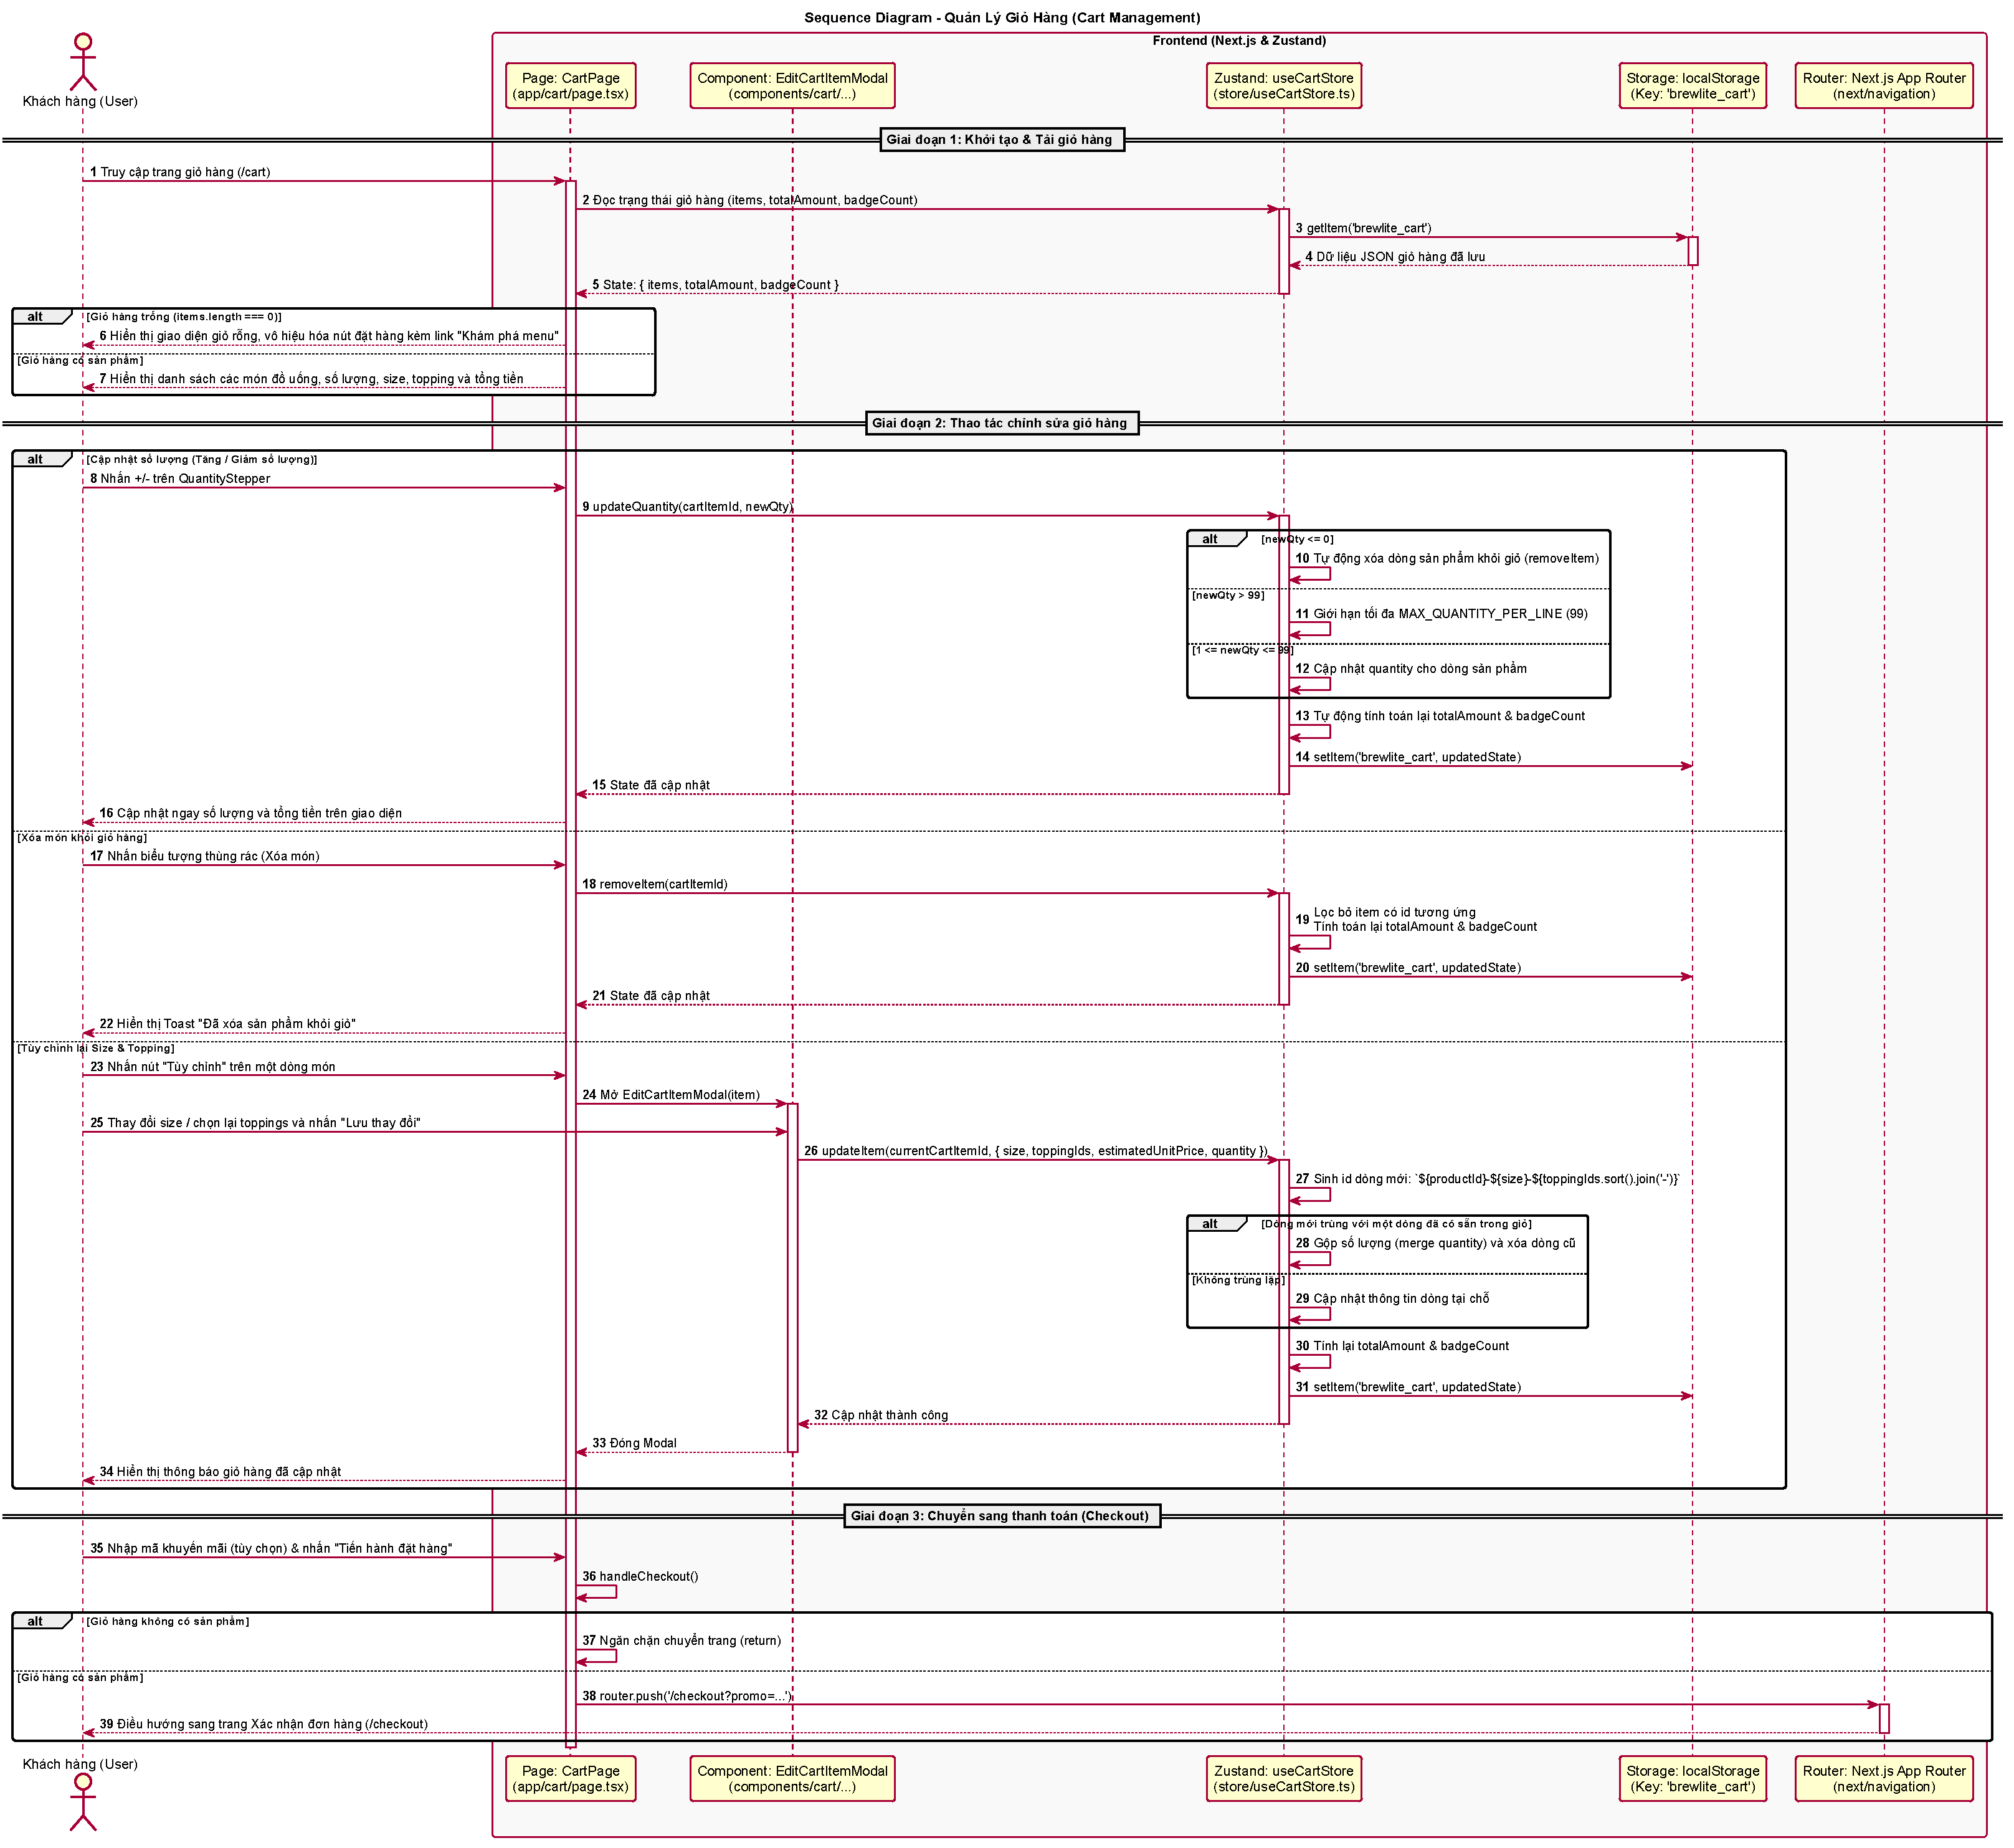
\includegraphics[width=\textwidth, height=0.80\textheight, keepaspectratio]{figures/sequence-cart.pdf}
    \caption{Sơ đồ Tuần tự - Phân hệ Giỏ hàng (Client-side Architecture)}
    \label{fig:sequence-cart}
\end{figure}

\clearpage
\subsection{Hợp đồng API và Ánh xạ Cơ sở dữ liệu}
\begin{itemize}
    \item \textbf{Đặc tính kỹ thuật (FE-Only):} Giỏ hàng trong BrewLite hoạt động hoàn toàn ở phía máy khách (\textit{Frontend-only}). Không có API endpoint riêng trên Backend và không tạo bản ghi trong cơ sở dữ liệu cho giỏ hàng tạm thời.
    \item \textbf{Cấu trúc đối tượng lưu trữ (\texttt{CartItem}):}
    Mỗi phần tử giỏ hàng được định danh bởi một khóa duy nhất sinh ra từ tổ hợp thuộc tính (\texttt{productId}, \texttt{size}, \texttt{sweetness}, \texttt{ice}, danh sách \texttt{toppings}):
    \begin{itemize}
        \item \texttt{id}: Mã duy nhất của món trong giỏ.
        \item \texttt{productId}: ID sản phẩm tham chiếu.
        \item \texttt{name}, \texttt{image}: Thông tin hiển thị.
        \item \texttt{size}, \texttt{sweetness}, \texttt{ice}: Các tùy biến đã chọn.
        \item \texttt{toppings}: Danh sách topping kèm giá đơn vị.
        \item \texttt{quantity}: Số lượng đặt (\(\ge 1\)).
        \item \texttt{unitPrice}: Đơn giá đã bao gồm phụ thu kích cỡ.
        \item \texttt{subtotal}: Tổng tiền của dòng món = \((unitPrice + \sum toppingPrice) \times quantity\).
    \end{itemize}
\end{itemize}

\subsection{Kịch bản Kiểm thử (Test Cases)}
\begin{table}[H]
\centering
\small
\caption{Tóm lược các Ca kiểm thử tiêu biểu - Phân hệ Giỏ hàng}
\label{tab:tc-cart}
\begin{tabularx}{\textwidth}{llp{2.6cm}p{3cm}Xc}
\toprule
\textbf{Mã TC} & \textbf{Loại} & \textbf{Tiền điều kiện} & \textbf{Endpoint / Màn hình} & \textbf{Kết quả mong đợi} & \textbf{Trạng thái} \\
\midrule
\texttt{TC-CART-UI-01} & Giao diện & Giỏ chưa có món & Màn hình \texttt{/cart} & Hiển thị thông báo giỏ hàng trống & Chưa chạy \\
\texttt{TC-CART-UI-02} & Nghiệp vụ & Đã thêm 1 món & Màn hình \texttt{/cart} & Hiển thị đúng tên, size, mức đường, đá, topping & Chưa chạy \\
\texttt{TC-CART-UI-03} & Nghiệp vụ & Đang có món & Nút tăng/giảm & Cập nhật số lượng và tự động tính lại tổng tiền & Chưa chạy \\
\texttt{TC-CART-UI-04} & Nghiệp vụ & Đang có món & Nút xóa món & Món bị loại bỏ khỏi danh sách, tính lại tiền & Chưa chạy \\
\bottomrule
\end{tabularx}
\end{table}

\subsection{Giao diện Người dùng}
\begin{figure}[H]
    \centering
    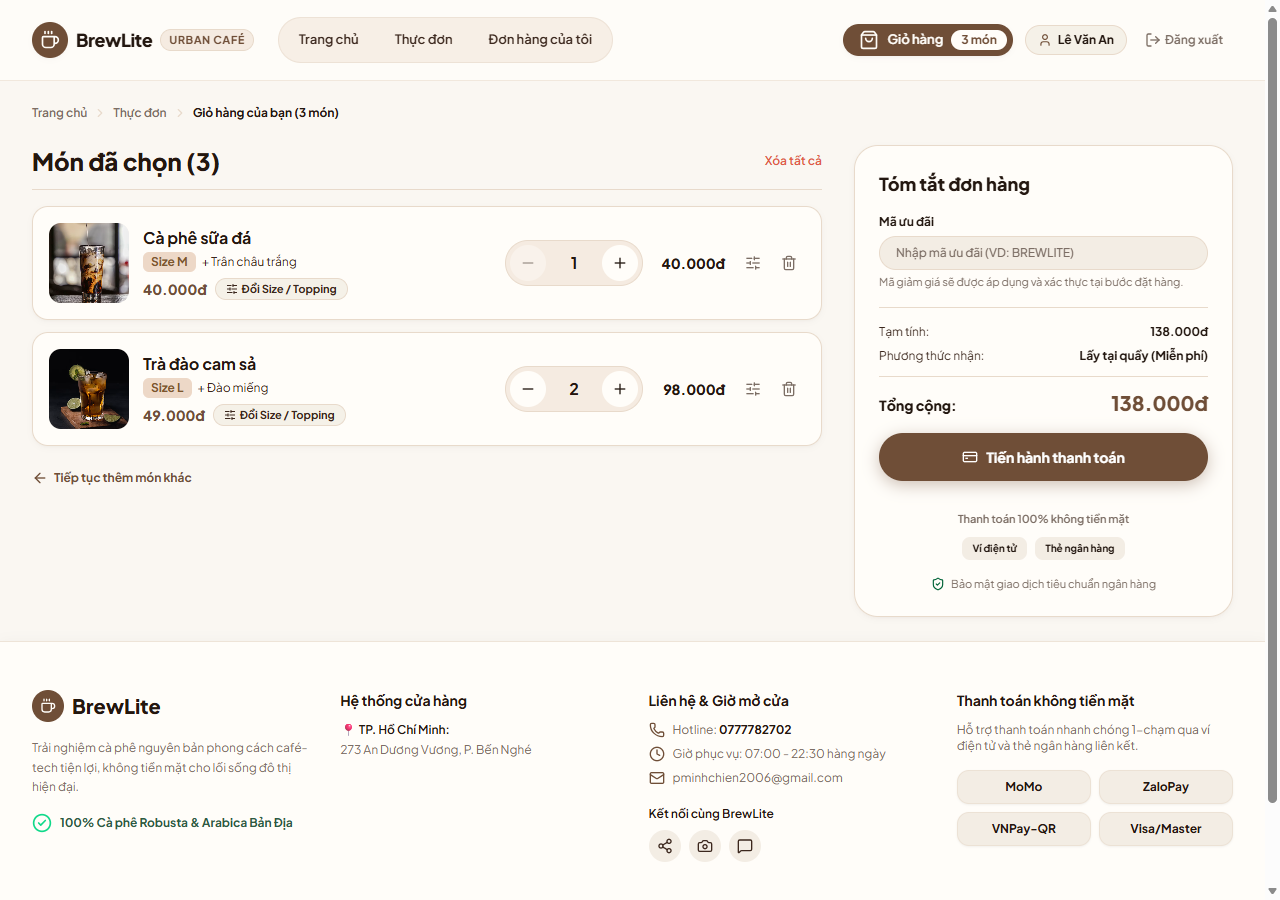
\includegraphics[width=0.92\textwidth]{figures/ui-cart.png}
    \caption{Giao diện Quản lý Giỏ hàng và Điều chỉnh số lượng BrewLite}
    \label{fig:ui-cart}
\end{figure}

\section{Phân hệ Đặt hàng (Order)}

\subsection{Đặc tả Use Case}
Phân hệ Đặt hàng là hạt nhân nghiệp vụ của hệ thống BrewLite, chịu trách nhiệm chuyển hóa các sản phẩm trong giỏ hàng thành đơn hàng chính thức. Phân hệ tích hợp các dịch vụ tính giá (\texttt{PricingService}), kiểm tra và áp dụng khuyến mãi (\texttt{PromotionsService}), tích lũy điểm thành viên (\texttt{LoyaltyService}) và kiểm soát kho bằng khóa lạc quan (\texttt{Optimistic Locking}). Sơ đồ Use Case được minh họa tại Hình~\ref{fig:usecase-order}.

\begin{figure}[htbp]
    \centering
    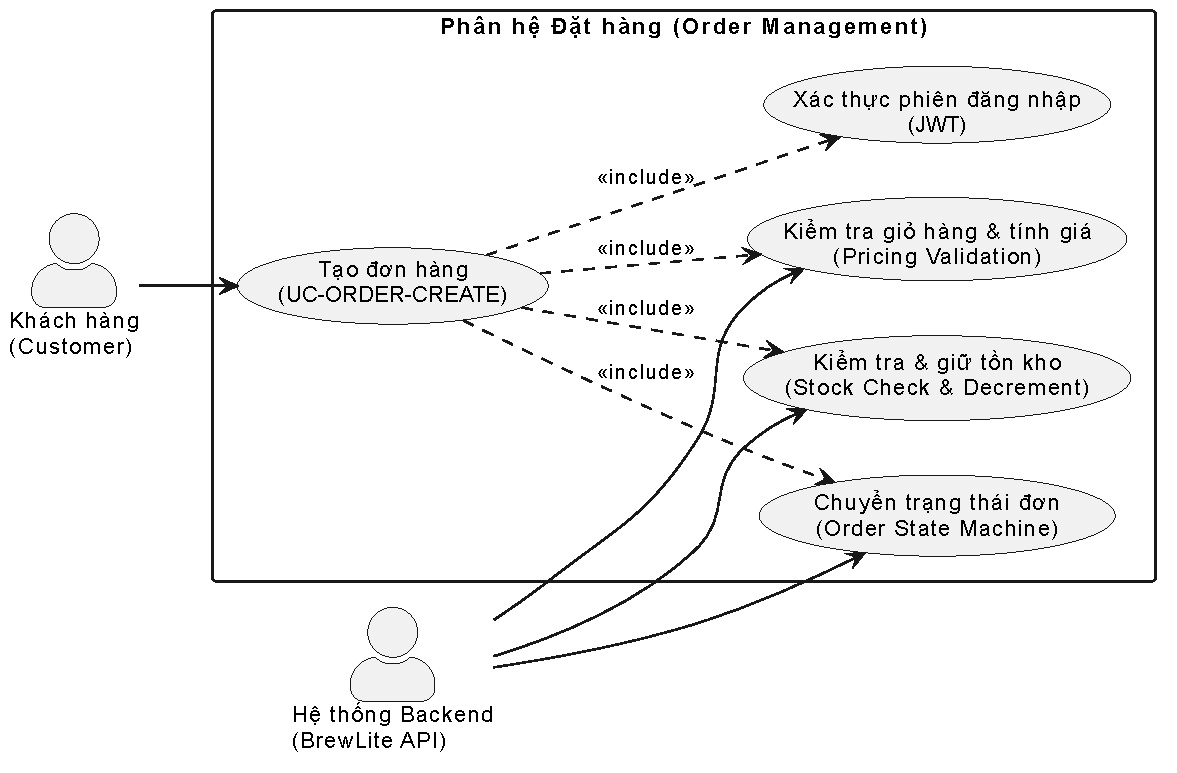
\includegraphics[width=0.75\textwidth]{figures/usecase-order.pdf}
    \caption{Sơ đồ Use Case - Phân hệ Đặt hàng}
    \label{fig:usecase-order}
\end{figure}

\begin{table}[htbp]
\centering
\small
\caption{Đặc tả Use Case: Tạo đơn hàng trực tuyến (UC-ORD-01)}
\label{tab:uc-spec-order}
\begin{tabularx}{\textwidth}{p{2.8cm}X}
\toprule
\textbf{Mục} & \textbf{Chi tiết Đặc tả} \\
\midrule
\textbf{Actor} & Khách hàng đã đăng nhập (Registered Customer) \\
\midrule
\textbf{Tiền điều kiện} & Khách hàng đã đăng nhập (mang Bearer JWT Token); giỏ hàng có ít nhất 1 sản phẩm. \\
\midrule
\textbf{Hậu điều kiện} & Bản ghi đơn hàng mới được tạo ở trạng thái \texttt{PENDING}; tồn kho sản phẩm được cập nhật; voucher được áp dụng; bản ghi lịch sử trạng thái được khởi tạo. \\
\midrule
\textbf{Luồng chính} & 
1. Khách hàng từ giỏ hàng nhấn "Tiến hành đặt hàng" đến trang Checkout (\texttt{/checkout}).\newline
2. Khách hàng nhập mã giảm giá (ví dụ \texttt{WELCOME10}) nếu có.\newline
3. Nhấn nút "Xác nhận đặt hàng".\newline
4. Giao diện gửi request \texttt{POST /api/v1/orders} kèm Bearer Token.\newline
5. Backend khởi động Interactive Transaction (\texttt{prisma.\$transaction}):\newline
\quad a. Kiểm tra từng sản phẩm, đối chiếu \texttt{version} và số lượng tồn kho \texttt{stock}.\newline
\quad b. Tính giá cơ bản, phụ thu size và giá topping qua \texttt{PricingService}.\newline
\quad c. Thẩm định mã giảm giá và tính số tiền giảm trừ qua \texttt{PromotionsService}.\newline
\quad d. Tính toán số điểm thưởng dự kiến tích lũy (\texttt{pointsEarned}).\newline
\quad e. Trừ tồn kho và tăng \texttt{version = version + 1} của sản phẩm.\newline
\quad f. Tạo bản ghi \texttt{orders}, các \texttt{order\_items} và \texttt{order\_item\_toppings}.\newline
\quad g. Thêm bản ghi vào \texttt{order\_status\_history} (chuyển trạng thái sang \texttt{PENDING}).\newline
6. Transaction commit thành công, trả về thông tin đơn hàng và mã số tự tăng \texttt{orderNumber} (ví dụ \#1042).\newline
7. Giao diện xóa giỏ hàng và điều hướng sang trang thanh toán (\texttt{/payment/[orderId]}). \\
\midrule
\textbf{Luồng ngoại lệ} & 
- Hết hàng hoặc tồn kho không đủ: Báo lỗi \texttt{400 Bad Request} ("Sản phẩm ... không đủ tồn kho"), rollback transaction.\newline
- Thiếu tồn kho hoặc xung đột phiên bản (Optimistic Lock Conflict): Báo lỗi \texttt{400 Bad Request} (\texttt{\"Insufficient stock or concurrent update...\"}), tự động rollback transaction.\newline
- Mã voucher không hợp lệ hoặc hết hạn: Báo lỗi \texttt{400 Bad Request} ("Mã giảm giá không hợp lệ").\newline
- Chưa đăng nhập: Báo lỗi \texttt{401 Unauthorized}, điều hướng về trang đăng nhập. \\
\bottomrule
\end{tabularx}
\end{table}

\subsection{Sơ đồ Hoạt động (Activity Diagram)}
Luồng hoạt động kiểm tra điều kiện tồn kho, tính giá và cam kết giao dịch tạo đơn được biểu diễn tại Hình~\ref{fig:activity-order}.

\begin{figure}[htbp]
    \centering
    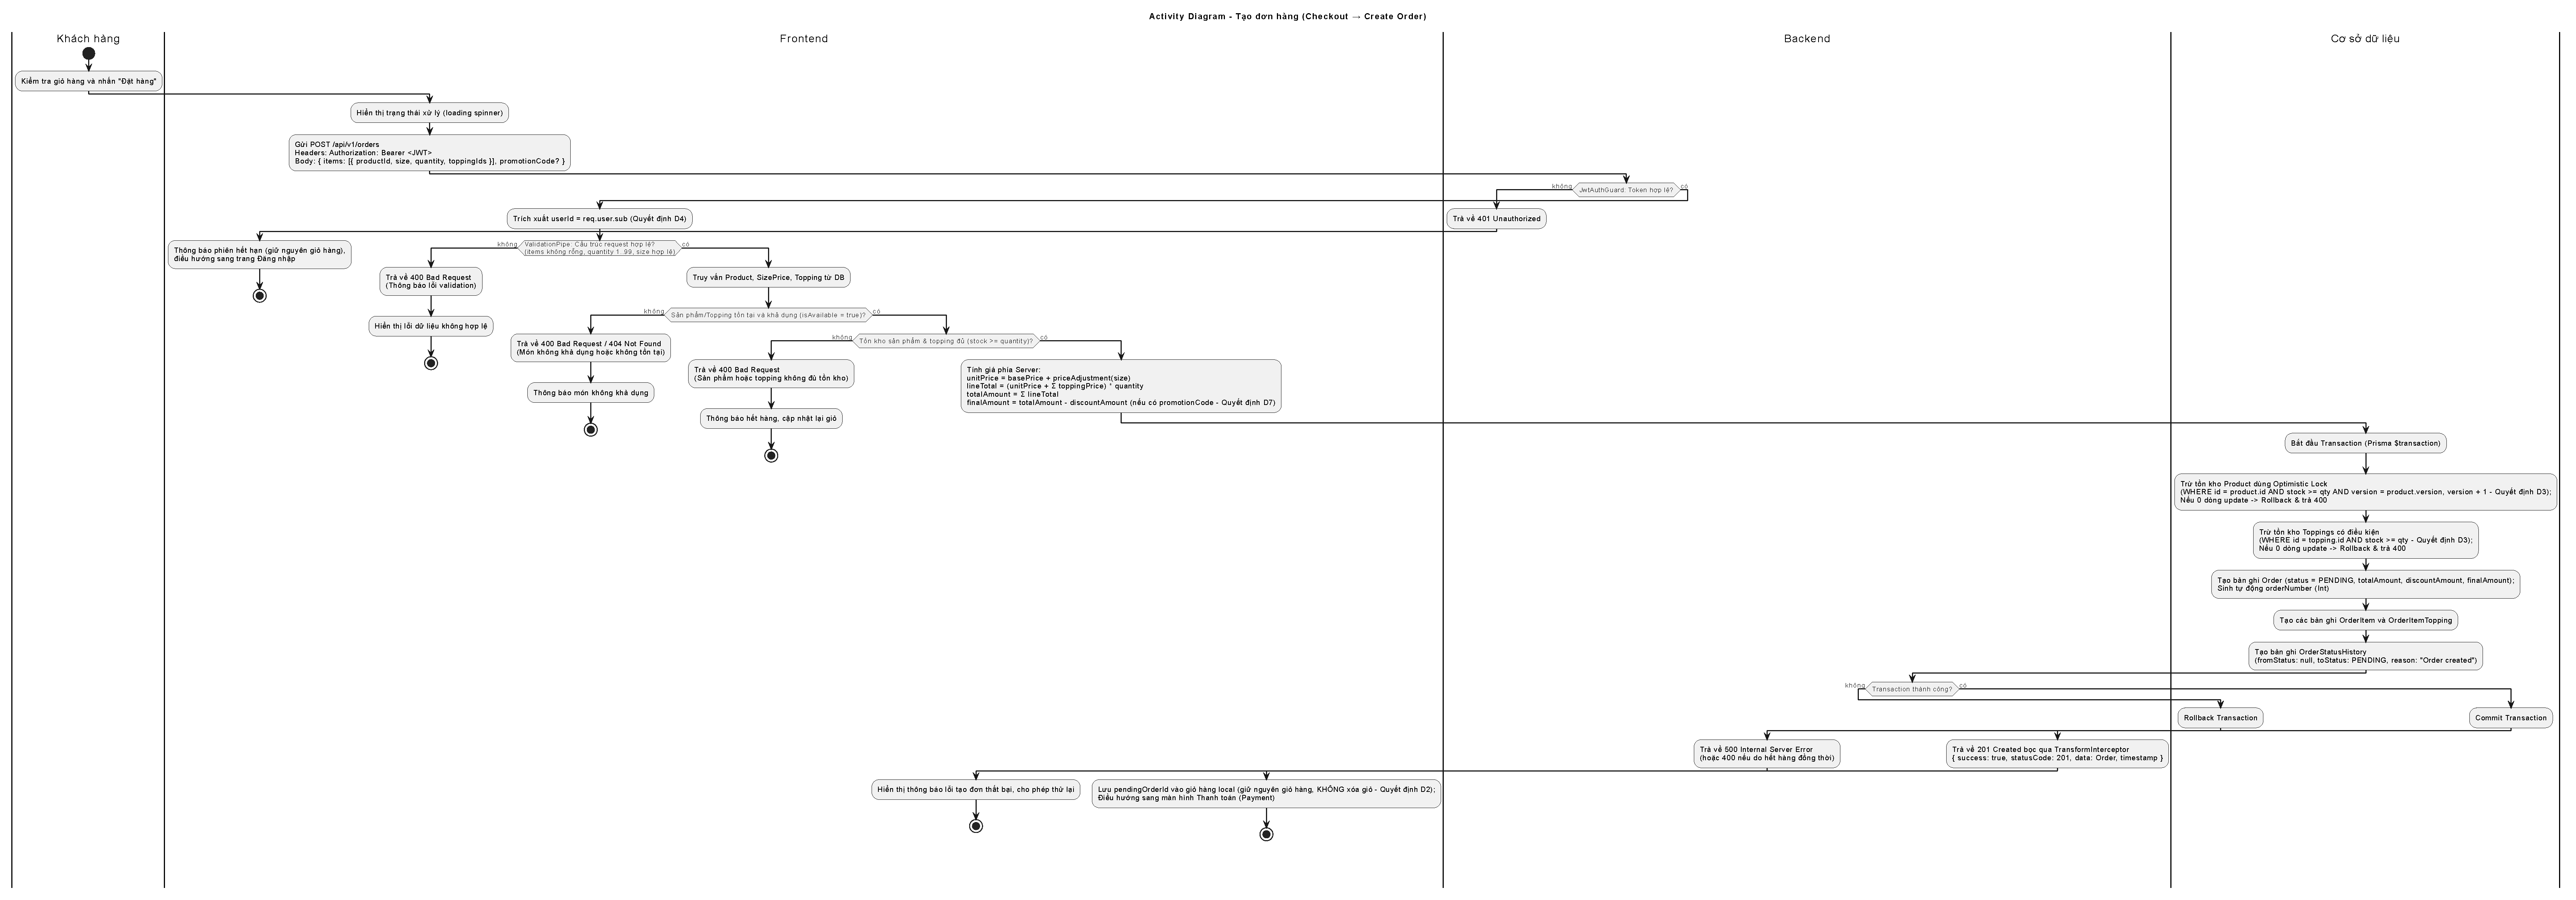
\includegraphics[width=0.75\textwidth]{figures/activity-order.pdf}
    \caption{Sơ đồ Hoạt động - Phân hệ Đặt hàng}
    \label{fig:activity-order}
\end{figure}

\subsection{Sơ đồ Tuần tự (Sequence Diagram)}
Sơ đồ Tuần tự minh họa chi tiết toàn bộ các lời gọi dịch vụ phối hợp trong một transaction tạo đơn hàng tại Hình~\ref{fig:sequence-order}.

\begin{figure}[htbp]
    \centering
    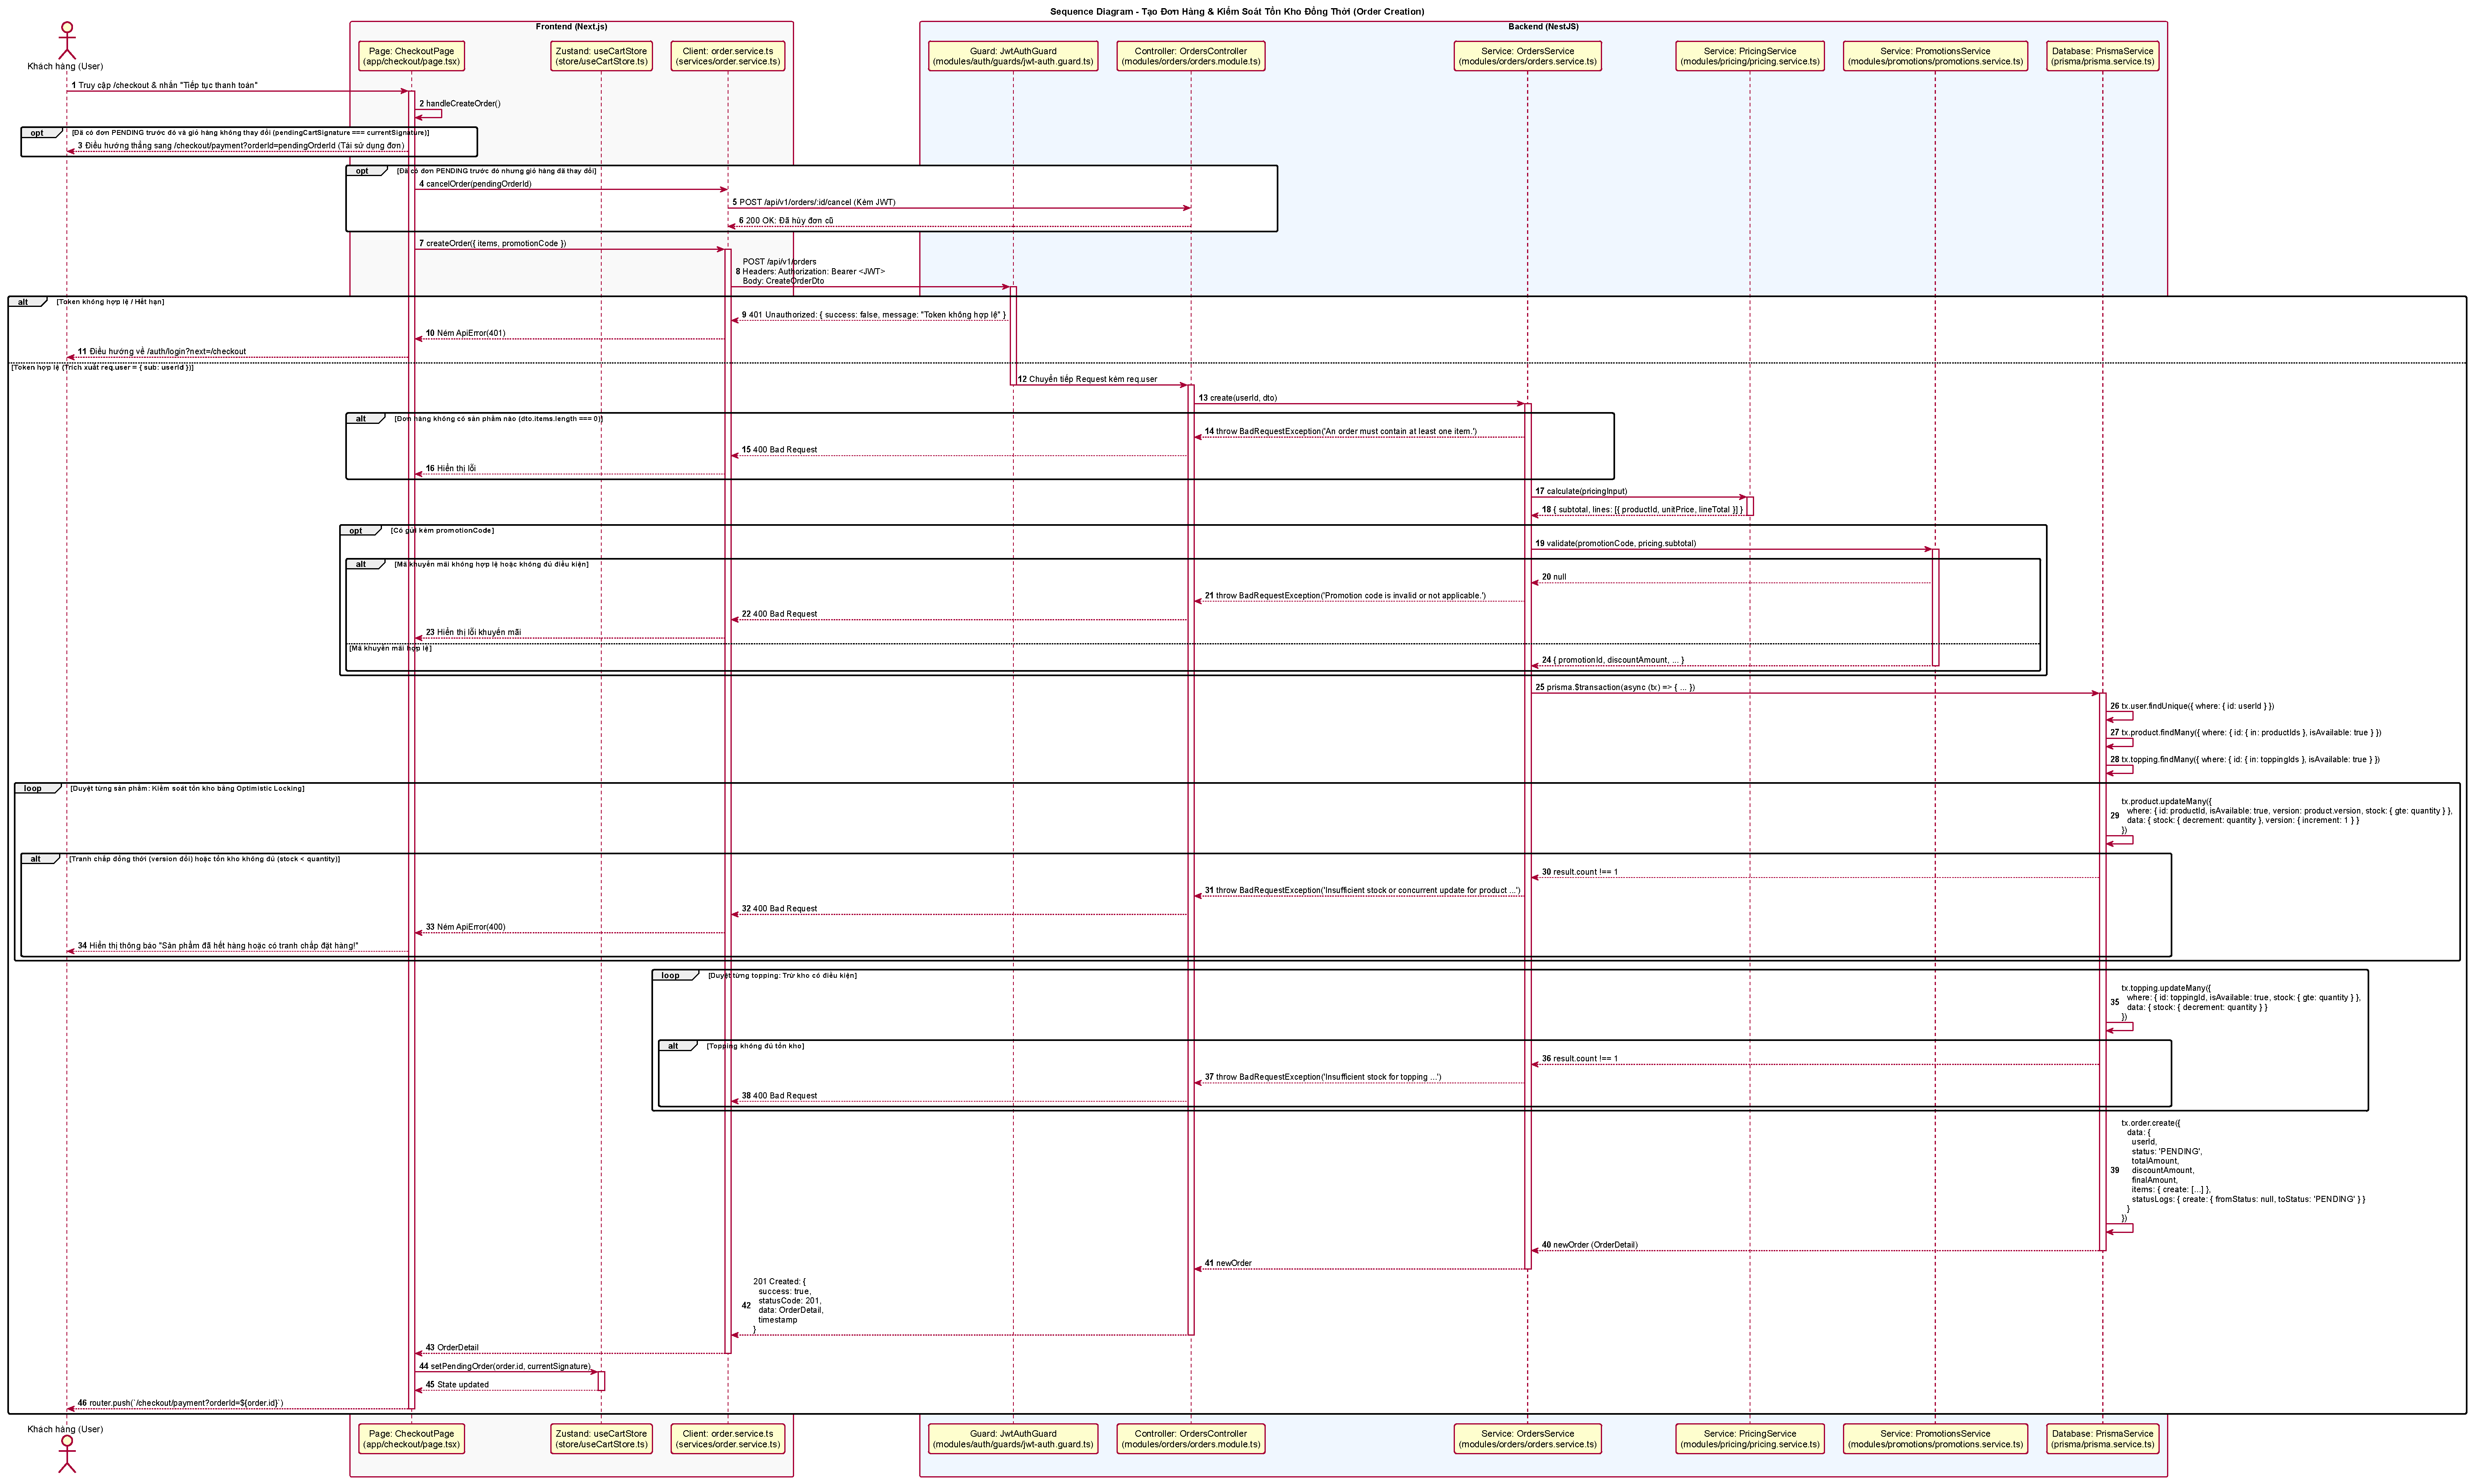
\includegraphics[width=0.9\textwidth]{figures/sequence-order.pdf}
    \caption{Sơ đồ Tuần tự - Phân hệ Đặt hàng (Interactive Transaction \& Pricing Engine)}
    \label{fig:sequence-order}
\end{figure}

\subsection{Hợp đồng API (API Contract)}
\begin{table}[htbp]
\centering
\small
\caption{Danh mục API Endpoints - Phân hệ Đặt hàng}
\label{tab:api-order}
\begin{tabularx}{\textwidth}{llp{4.5cm}X}
\toprule
\textbf{Phương thức} & \textbf{Endpoint} & \textbf{Mô tả Request Payload} & \textbf{Phản hồi chính} \\
\midrule
\texttt{POST} & \texttt{/api/v1/orders} & 
\texttt{\{items: [\{productId, size, quantity, toppings\}], promotionCode?\}} (Header: \texttt{Authorization: Bearer <JWT>}) & 
\texttt{201 Created}: Trả về đơn hàng mới tạo với cấu trúc bọc chuẩn \texttt{TransformInterceptor}. Lỗi: \texttt{400 Bad Request}, \texttt{401 Unauthorized}. \\
\texttt{GET} & \texttt{/api/v1/orders/:id} & Tham số \texttt{id} của đơn hàng (Header: Bearer Token) & 
\texttt{200 OK}: Chi tiết đơn hàng, danh sách món, trạng thái xử lý và các lần thử thanh toán. \\
\bottomrule
\end{tabularx}
\end{table}

\subsection{Ánh xạ Cơ sở dữ liệu (Database Mapping)}
Quá trình tạo đơn hàng thực thi nguyên tử trong một \texttt{prisma.\$transaction}:
\begin{lstlisting}[language=SQL]
-- 1. Kiem tra va cap nhat ton kho voi Optimistic Locking
UPDATE products 
SET stock = stock - :quantity, version = version + 1
WHERE id = :productId AND version = :currentVersion AND stock >= :quantity;

-- 2. Tao ban ghi don hang chinh thuc
INSERT INTO orders (id, order_number, user_id, status, total_amount, discount_amount, final_amount, points_earned, version, created_at, updated_at)
VALUES (cuid(), nextval('orders_order_number_seq'), :userId, 'PENDING', :totalAmount, :discountAmount, :finalAmount, :pointsEarned, 0, NOW(), NOW());

-- 3. Tao cac chi tiet don hang va luu snapshot gia
INSERT INTO order_items (id, order_id, product_id, size, quantity, unit_price, line_total)
VALUES (cuid(), :orderId, :productId, :size, :quantity, :unitPrice, :lineTotal);

-- 4. Ghi nhat ky trang thai ban dau
INSERT INTO order_status_history (id, order_id, from_status, to_status, changed_by, created_at)
VALUES (cuid(), :orderId, NULL, 'PENDING', 'system', NOW());
\end{lstlisting}

\subsection{Kịch bản Kiểm thử (Test Cases)}
\begin{table}[htbp]
\centering
\small
\caption{Tóm lược các Ca kiểm thử tiêu biểu - Phân hệ Đặt hàng}
\label{tab:tc-order}
\begin{tabularx}{\textwidth}{llp{2.6cm}p{3cm}Xc}
\toprule
\textbf{Mã TC} & \textbf{Loại} & \textbf{Tiền điều kiện} & \textbf{Endpoint / Màn hình} & \textbf{Kết quả mong đợi} & \textbf{Trạng thái} \\
\midrule
\texttt{TC-ORD-API-01} & Hợp lệ & Đủ tồn kho, có token & \texttt{POST /orders} & HTTP 201, tạo đơn trạng thái PENDING, trừ kho & Chưa chạy \\
\texttt{TC-ORD-API-03} & Lỗi & Tồn kho không đủ & \texttt{POST /orders} & HTTP 400, rollback transaction, không trừ kho & Chưa chạy \\
\texttt{TC-ORD-API-04} & Lỗi & Xung đột version (Optimistic) & \texttt{POST /orders} & HTTP 400 Bad Request (\"Insufficient stock or concurrent update...\"), rollback & Đạt \\
\texttt{TC-ORD-API-06} & Hợp lệ & Áp voucher WELCOME10 & \texttt{POST /orders} & Giảm 10\% (tối đa 20k), finalAmount chính xác & Đạt \\
\texttt{TC-ORD-UI-01} & Giao diện & Đã đăng nhập & Trang \texttt{/checkout} & Hiển thị tóm tắt đơn, ô nhập voucher và nút đặt & Chưa chạy \\
\bottomrule
\end{tabularx}
\end{table}

\subsection{Giao diện Người dùng}
\begin{figure}[htbp]
    \centering
    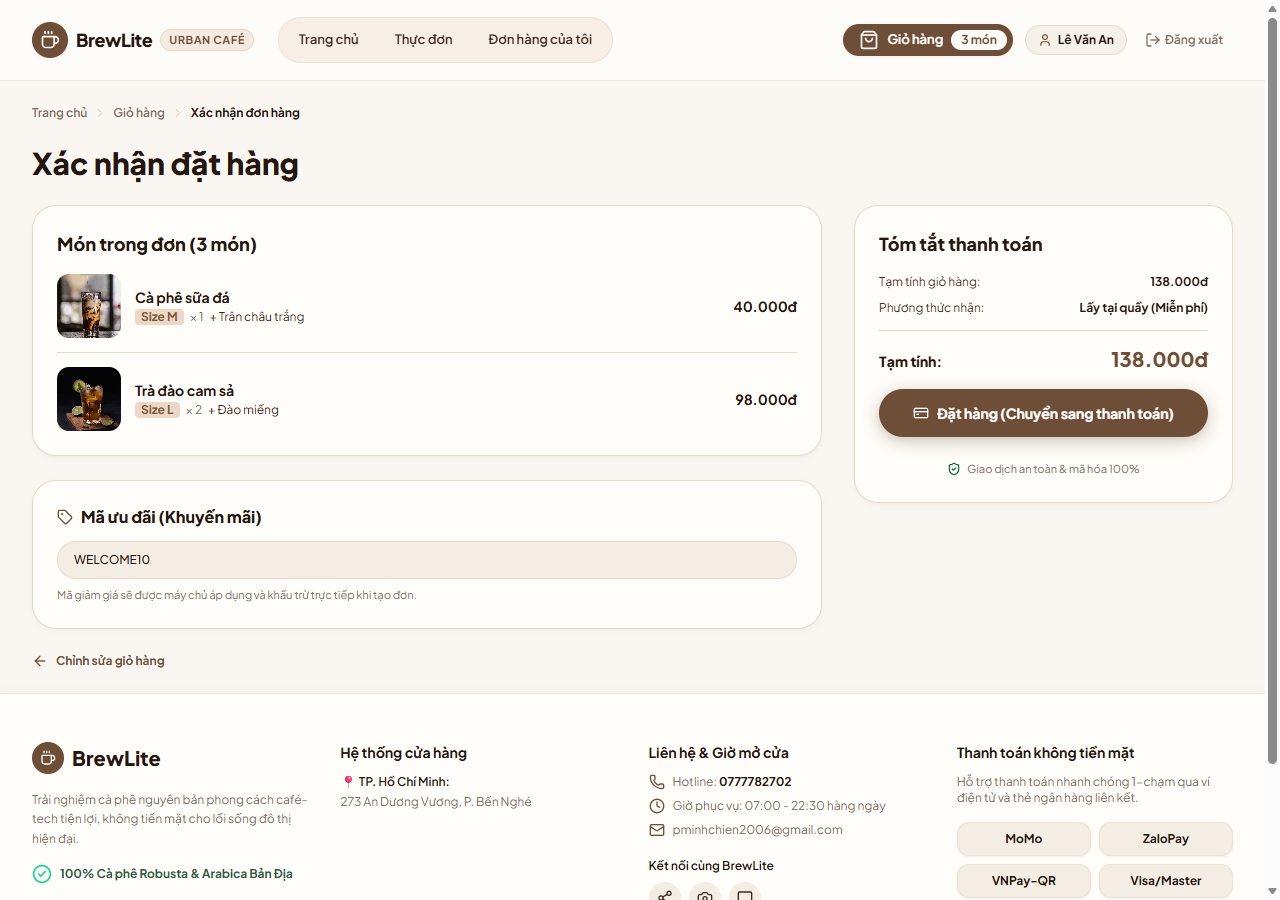
\includegraphics[width=0.92\textwidth]{figures/ui-checkout.png}
    \caption{Giao diện Xác nhận Đặt hàng và Áp dụng Khuyến mại}
    \label{fig:ui-order}
\end{figure}

\clearpage
\section{Phân hệ Thanh toán (Payment)}

\subsection{Đặc tả Use Case}
Phân hệ Thanh toán chịu trách nhiệm tiếp nhận và xử lý giao dịch tài chính cho các đơn hàng đang ở trạng thái chờ. Phân hệ được thiết kế với cơ chế an toàn cấp cao: bảo vệ giao dịch bất biến (\textit{Idempotency}) để chống trùng lặp tiền khi người dùng nhấp đúp hoặc xảy ra lỗi chập chờn mạng, đồng thời hỗ trợ nhiều lượt thử lại (\textit{Retry}) cho cùng một đơn hàng thông qua quan hệ 1-N giữa \texttt{Order} và \texttt{Payment}. Sơ đồ Use Case được minh họa tại Hình~\ref{fig:usecase-payment}.

\begin{figure}[H]
    \centering
    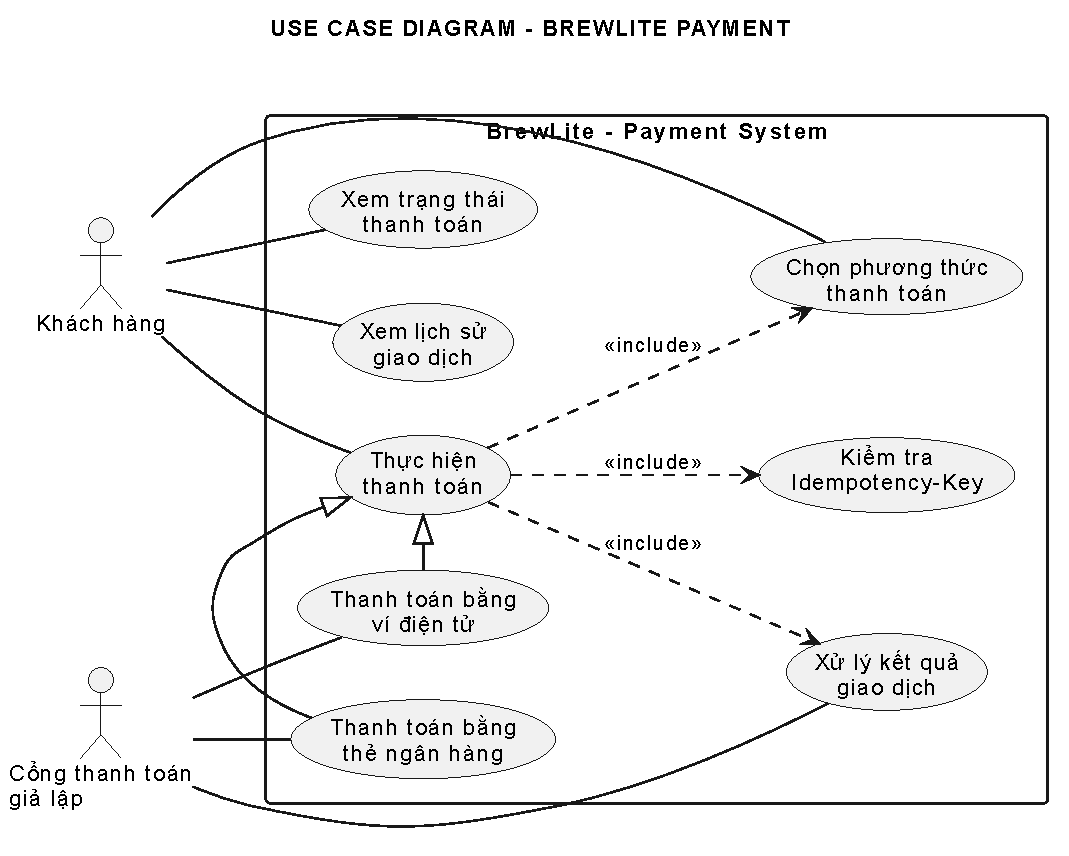
\includegraphics[width=0.75\textwidth]{figures/usecase-payment.pdf}
    \caption{Sơ đồ Use Case - Phân hệ Thanh toán}
    \label{fig:usecase-payment}
\end{figure}

\begin{table}[H]
\centering
\small
\caption{Đặc tả Use Case: Thực hiện Thanh toán Trực tuyến (UC-PAY-01)}
\label{tab:uc-spec-payment}
\begin{tabularx}{\textwidth}{p{2.8cm}X}
\toprule
\textbf{Mục} & \textbf{Chi tiết Đặc tả} \\
\midrule
\textbf{Actor} & Khách hàng đã đăng nhập, Cổng thanh toán giả lập (Mock Gateway) \\
\midrule
\textbf{Tiền điều kiện} & Đơn hàng tồn tại ở trạng thái \texttt{PENDING}; chưa được thanh toán thành công. \\
\midrule
\textbf{Hậu điều kiện} & Bản ghi thanh toán được lưu trữ; trạng thái đơn hàng chuyển thành \texttt{PAID}; điểm loyalty được cộng vào tài khoản khách hàng. \\
\midrule
\textbf{Luồng chính} & 
1. Khách hàng truy cập trang thanh toán \texttt{/payment/[orderId]}.\newline
2. Chọn phương thức thanh toán: Thẻ ngân hàng (\texttt{BANK\_CARD}) hoặc Ví điện tử (\texttt{E\_WALLET}).\newline
3. Nhấn "Thanh toán ngay".\newline
4. Trình duyệt tự động sinh mã UUID \texttt{Idempotency-Key} duy nhất và gửi request \texttt{POST /api/v1/payments}.\newline
5. PaymentsService kiểm tra \texttt{idempotencyKey}:\newline
\quad a. Nếu khóa đã tồn tại trong DB: Gọi \texttt{replayExistingPayment()} đối chiếu mã băm SHA-256 trên \texttt{\{orderId, method\}}. Nếu trùng khớp, trả lại kết quả đã lưu mà không gọi lại Mock Gateway; nếu sai lệch tải trọng, ném ngoại lệ \texttt{409 Conflict}.\newline
\quad b. Nếu là khóa mới: Khởi tạo giao dịch \texttt{payments} trong \texttt{prisma.\$transaction} với trạng thái \texttt{PENDING} và lưu mã băm \texttt{requestHash}.\newline
\quad c. Xử lý tranh chấp đồng thời: Nếu hai request cùng gửi một khóa, lỗi trùng khóa Unique (\texttt{P2002}) được bắt trong khối \texttt{catch}, tự động truy vấn lại giao dịch vừa tạo và phát lại (\textit{replay}) kết quả an toàn.\newline
6. Backend gọi Mock Payment Gateway để xác thực giao dịch.\newline
7. Khi Gateway phản hồi thành công (\texttt{SUCCESS}):\newline
\quad a. Cập nhật bản ghi \texttt{payments} thành \texttt{SUCCESS} kèm \texttt{transactionRef}.\newline
\quad b. Cập nhật đơn hàng: \texttt{status = PAID}, \texttt{paidAt = NOW()}.\newline
\quad c. Cộng điểm tích lũy mới vào \texttt{users.loyalty\_points}.\newline
\quad d. Ghi nhận giao dịch cộng điểm vào \texttt{loyalty\_transactions} (type: \texttt{EARNED}).\newline
\quad e. Ghi nhật ký vào \texttt{order\_status\_history} (PENDING \(\to\) PAID).\newline
8. Giao diện thông báo thanh toán thành công và điều hướng sang trang Lịch sử đơn hàng. \\
\midrule
\textbf{Luồng ngoại lệ} & 
- Gateway từ chối hoặc giao dịch thất bại: Cập nhật bản ghi payment thành \texttt{FAILED}, đơn hàng chuyển sang \texttt{PAYMENT\_FAILED}, cho phép khách hàng nhấn thử lại (tạo lượt payment mới).\newline
- Đơn hàng đã được thanh toán trước đó: Báo lỗi \texttt{400 Bad Request} ("Đơn hàng đã được thanh toán").\newline
- Trùng Idempotency-Key nhưng khác payload: Báo lỗi \texttt{409 Conflict} (\"Idempotency-Key đã được sử dụng với nội dung khác\"). \\
\bottomrule
\end{tabularx}
\end{table}

\clearpage
\subsection{Sơ đồ Hoạt động (Activity Diagram)}
Quy trình thẩm định Idempotency, gọi cổng thanh toán và xử lý kết quả giao dịch được mô tả tại Hình~\ref{fig:activity-payment}.

\begin{figure}[H]
    \centering
    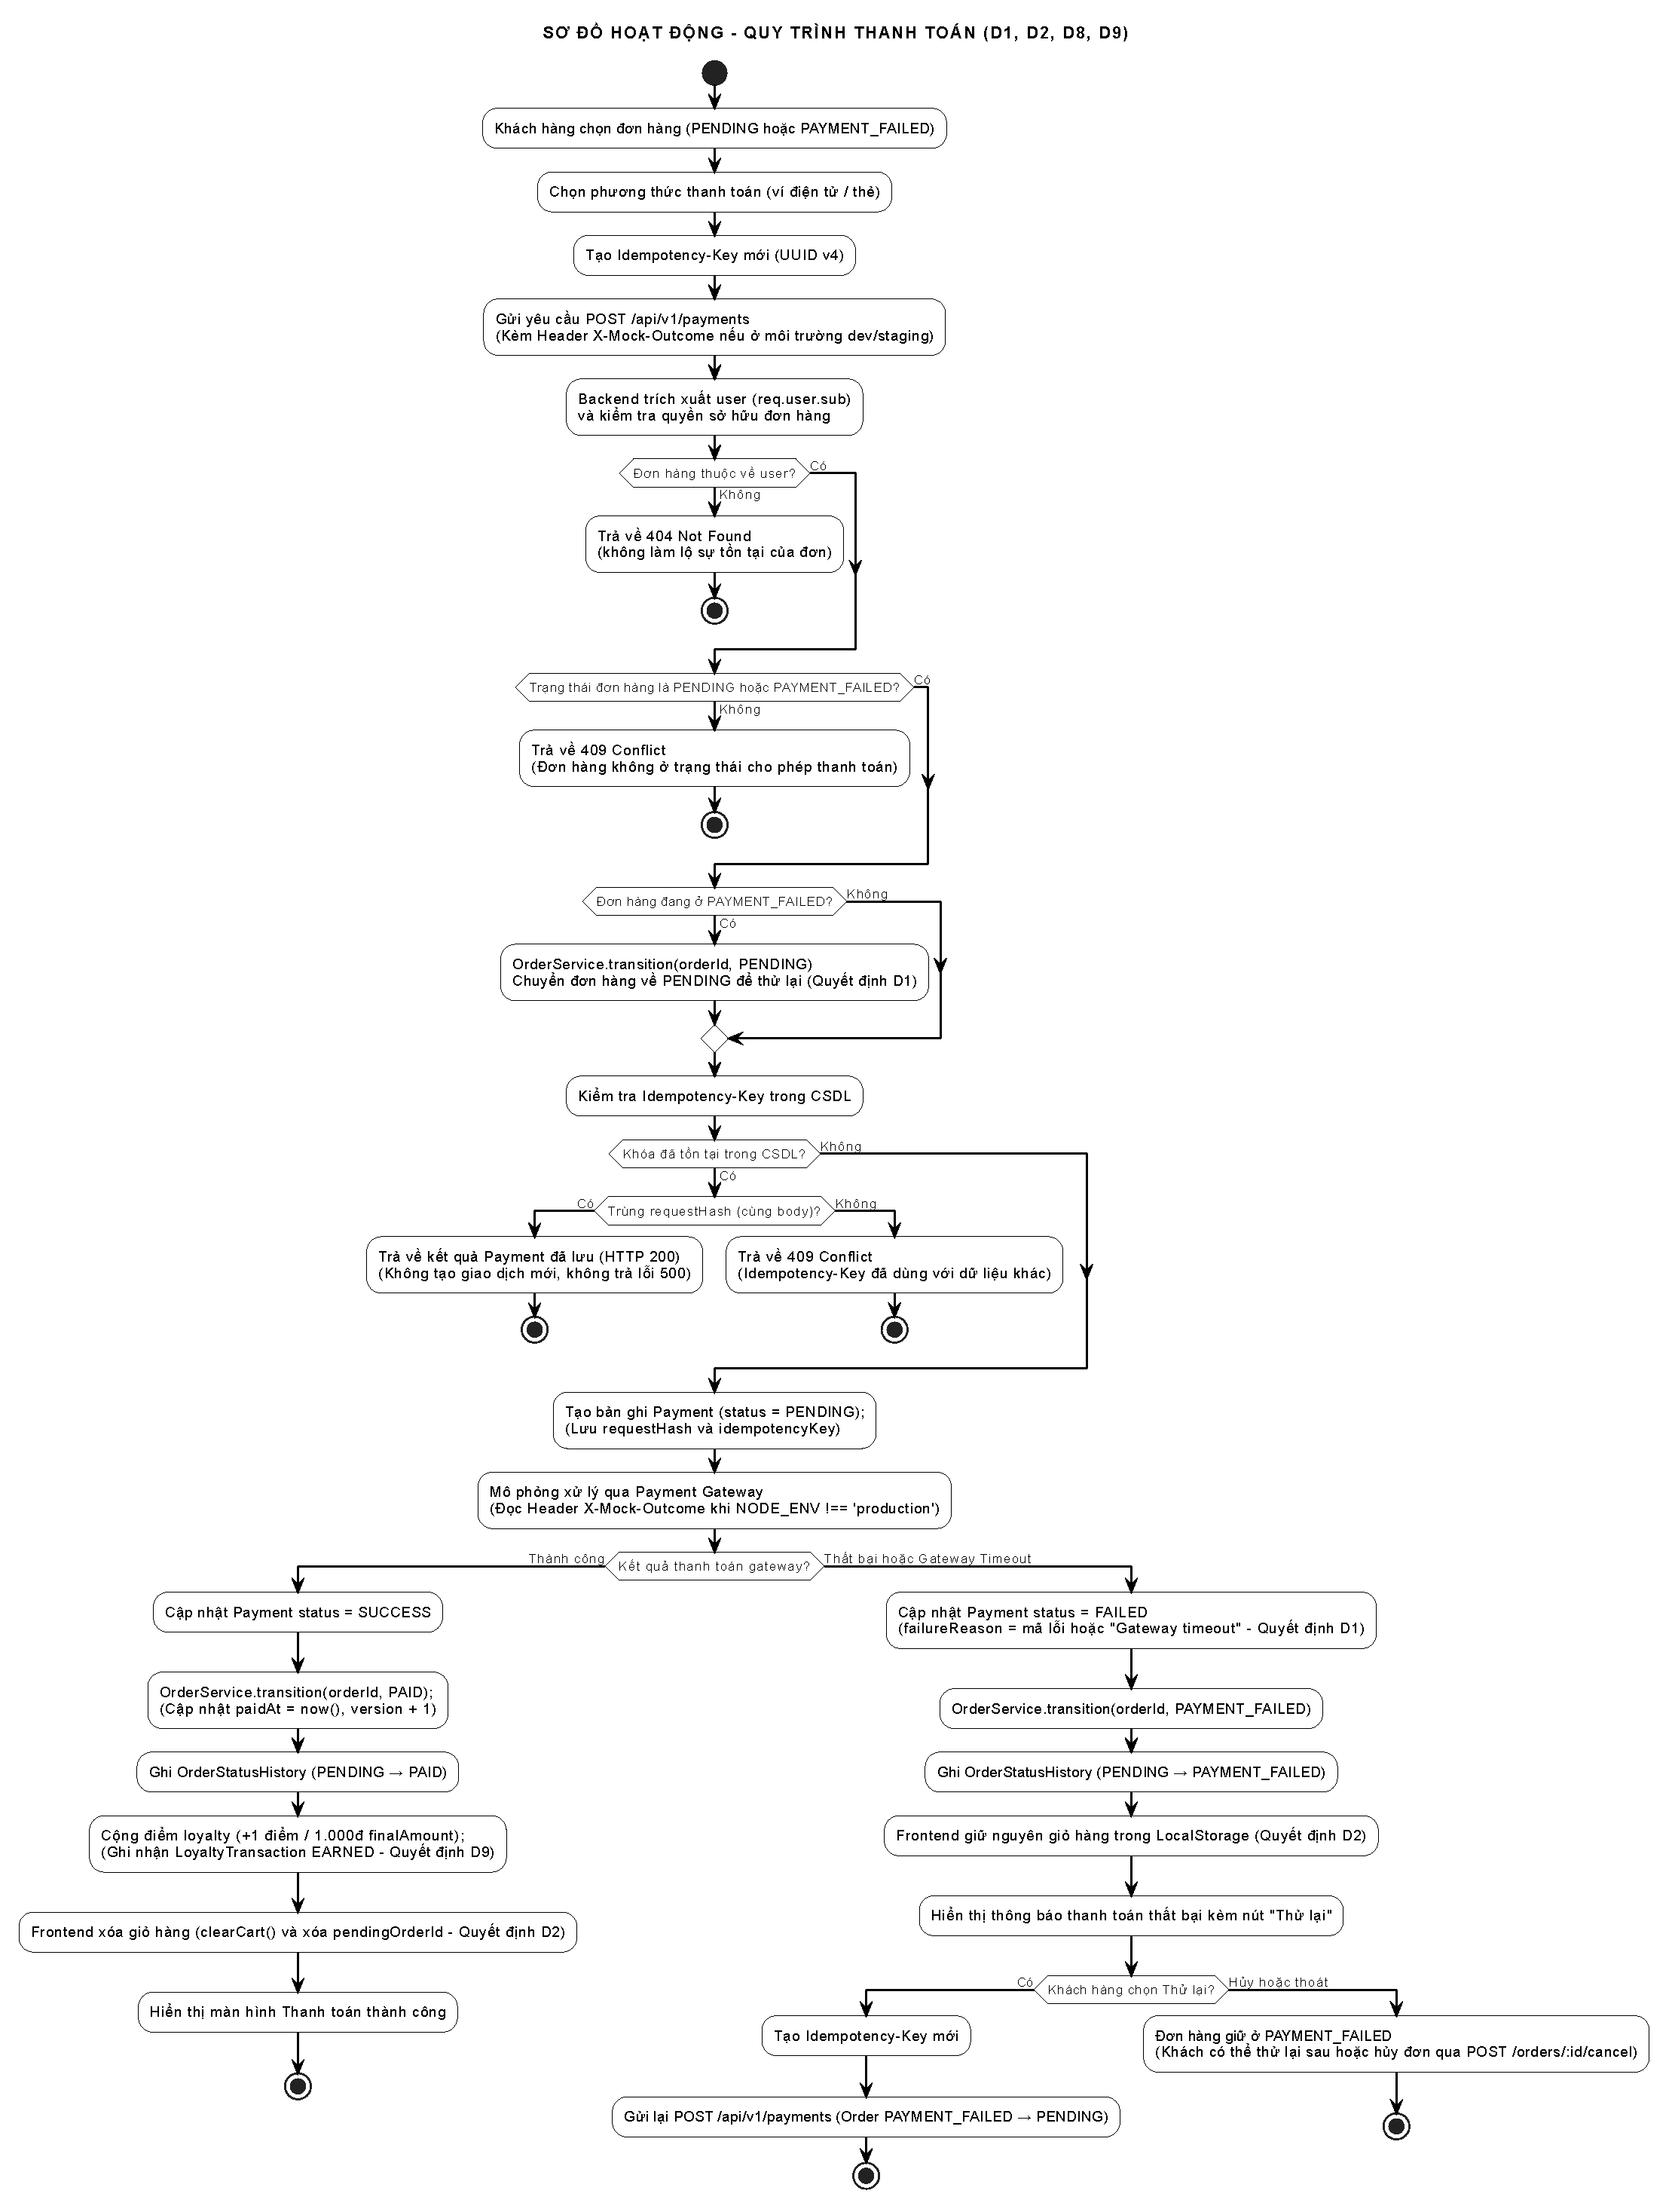
\includegraphics[width=\textwidth, height=0.80\textheight, keepaspectratio]{figures/activity-payment.pdf}
    \caption{Sơ đồ Hoạt động - Phân hệ Thanh toán}
    \label{fig:activity-payment}
\end{figure}

\clearpage
\subsection{Sơ đồ Tuần tự (Sequence Diagram)}
Sơ đồ Tuần tự phản ánh toàn diện các luồng tương tác giữa Frontend, PaymentsController, PaymentsService, Prisma DB và Mock Payment Gateway tại Hình~\ref{fig:sequence-payment}.

\begin{figure}[H]
    \centering
    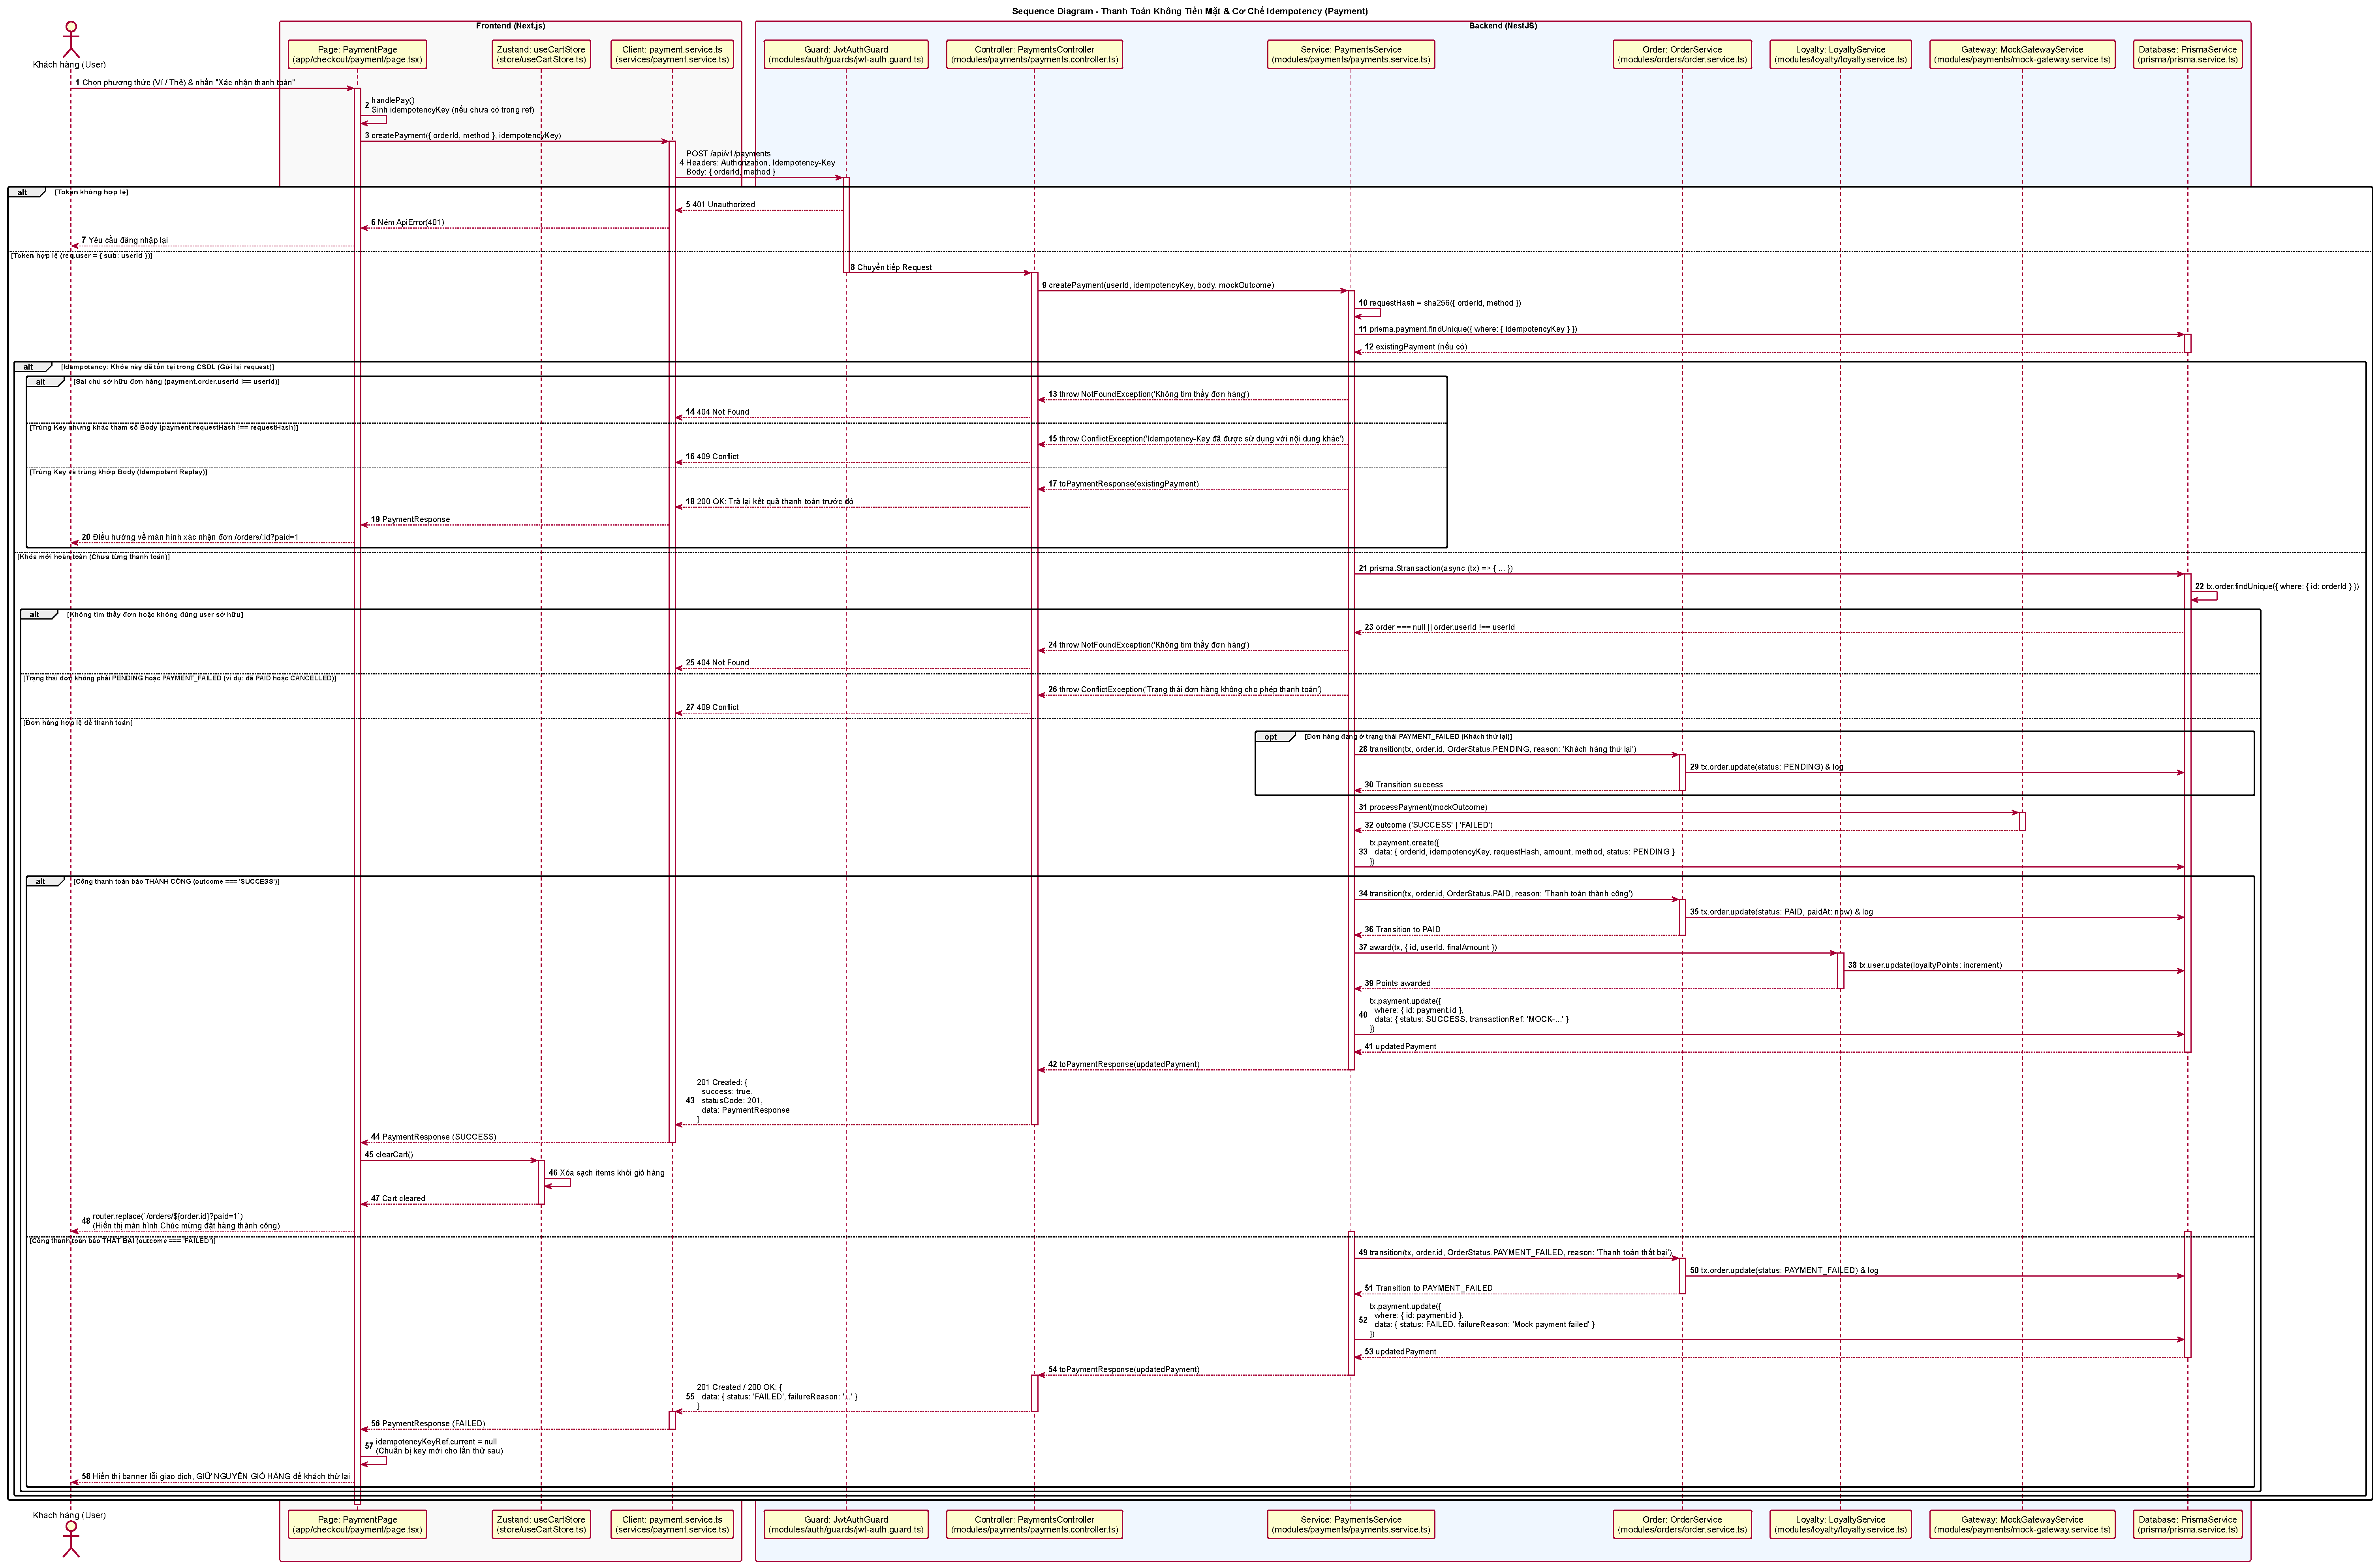
\includegraphics[width=\textwidth, height=0.80\textheight, keepaspectratio]{figures/sequence-payment.pdf}
    \caption{Sơ đồ Tuần tự - Phân hệ Thanh toán (Idempotent Flow \& Gateway Integration)}
    \label{fig:sequence-payment}
\end{figure}

\clearpage
\subsection{Hợp đồng API (API Contract)}
\begin{table}[H]
\centering
\small
\caption{Danh mục API Endpoints - Phân hệ Thanh toán}
\label{tab:api-payment}
\begin{tabularx}{\textwidth}{llp{4.5cm}X}
\toprule
\textbf{Phương thức} & \textbf{Endpoint} & \textbf{Headers \& Body} & \textbf{Phản hồi chính} \\
\midrule
\texttt{POST} & \texttt{/api/v1/payments} & 
Header: \texttt{Idempotency-Key: <UUID>}, Bearer Token.\newline Body: \texttt{\{orderId, method\}} & 
\texttt{200 OK}: Trả về chi tiết thanh toán thành công (hoặc kết quả phát lại). Lỗi: \texttt{400 Bad Request}, \texttt{401 Unauthorized}, \texttt{404 Not Found}, \texttt{409 Conflict} (sai lệch requestHash hoặc trạng thái đơn không hợp lệ). \\
\texttt{GET} & \texttt{/api/v1/payments/:id} & Tham số \texttt{id} bản ghi thanh toán & 
\texttt{200 OK}: Tra cứu trạng thái giao dịch thanh toán hiện tại. \\
\bottomrule
\end{tabularx}
\end{table}

\subsection{Ánh xạ Cơ sở dữ liệu (Database Mapping)}
\begin{itemize}
    \item \textbf{Cơ chế Idempotency:} Bảng \texttt{payments} sử dụng ràng buộc \texttt{@unique} trên trường \texttt{idempotency\_key} kết hợp cùng \texttt{request\_hash} sinh từ thuật toán SHA-256 trên nội dung JSON của body request:
    \begin{lstlisting}[language=SQL]
SELECT id, status, request_hash, transaction_ref 
FROM payments 
WHERE idempotency_key = :idempotencyKey;
    \end{lstlisting}
    \item \textbf{Cập nhật sau thanh toán thành công:} Thực thi trong transaction cập nhật đồng thời 4 bảng:
    \begin{lstlisting}[language=SQL]
UPDATE payments SET status = 'SUCCESS', transaction_ref = :ref WHERE id = :paymentId;
UPDATE orders SET status = 'PAID', paid_at = NOW() WHERE id = :orderId;
UPDATE users SET loyalty_points = loyalty_points + :pointsEarned WHERE id = :userId;
INSERT INTO loyalty_transactions (id, user_id, order_id, points, type, reason, created_at)
VALUES (cuid(), :userId, :orderId, :pointsEarned, 'EARNED', 'Tich diem tu don hang', NOW());
INSERT INTO order_status_history (id, order_id, from_status, to_status, changed_by, created_at)
VALUES (cuid(), :orderId, 'PENDING', 'PAID', 'payment_gateway', NOW());
    \end{lstlisting}
\end{itemize}

\subsection{Kịch bản Kiểm thử (Test Cases)}
\begin{table}[H]
\centering
\small
\caption{Tóm lược các Ca kiểm thử tiêu biểu - Phân hệ Thanh toán}
\label{tab:tc-payment}
\begin{tabularx}{\textwidth}{llp{2.6cm}p{3cm}Xc}
\toprule
\textbf{Mã TC} & \textbf{Loại} & \textbf{Tiền điều kiện} & \textbf{Endpoint / Màn hình} & \textbf{Kết quả mong đợi} & \textbf{Trạng thái} \\
\midrule
\texttt{TC-PAY-API-01} & Hợp lệ & Đơn PENDING, key mới & \texttt{POST /payments} & HTTP 200, status SUCCESS, đơn chuyển sang PAID & Chưa chạy \\
\texttt{TC-PAY-API-03} & Idempotent & Gửi lại cùng key & \texttt{POST /payments} & HTTP 200, trả về kết quả cũ, không gọi lại gateway & Chưa chạy \\
\texttt{TC-PAY-API-05} & Lỗi & Đơn đã thanh toán & \texttt{POST /payments} & HTTP 400, báo lỗi đơn hàng đã thanh toán & Chưa chạy \\
\texttt{TC-PAY-UI-01} & Giao diện & Đơn hàng chờ & Trang \texttt{/payment/[id]} & Hiển thị tổng tiền và 2 phương thức thẻ/ví & Chưa chạy \\
\bottomrule
\end{tabularx}
\end{table}

\subsection{Giao diện Người dùng}
\begin{figure}[H]
    \centering
    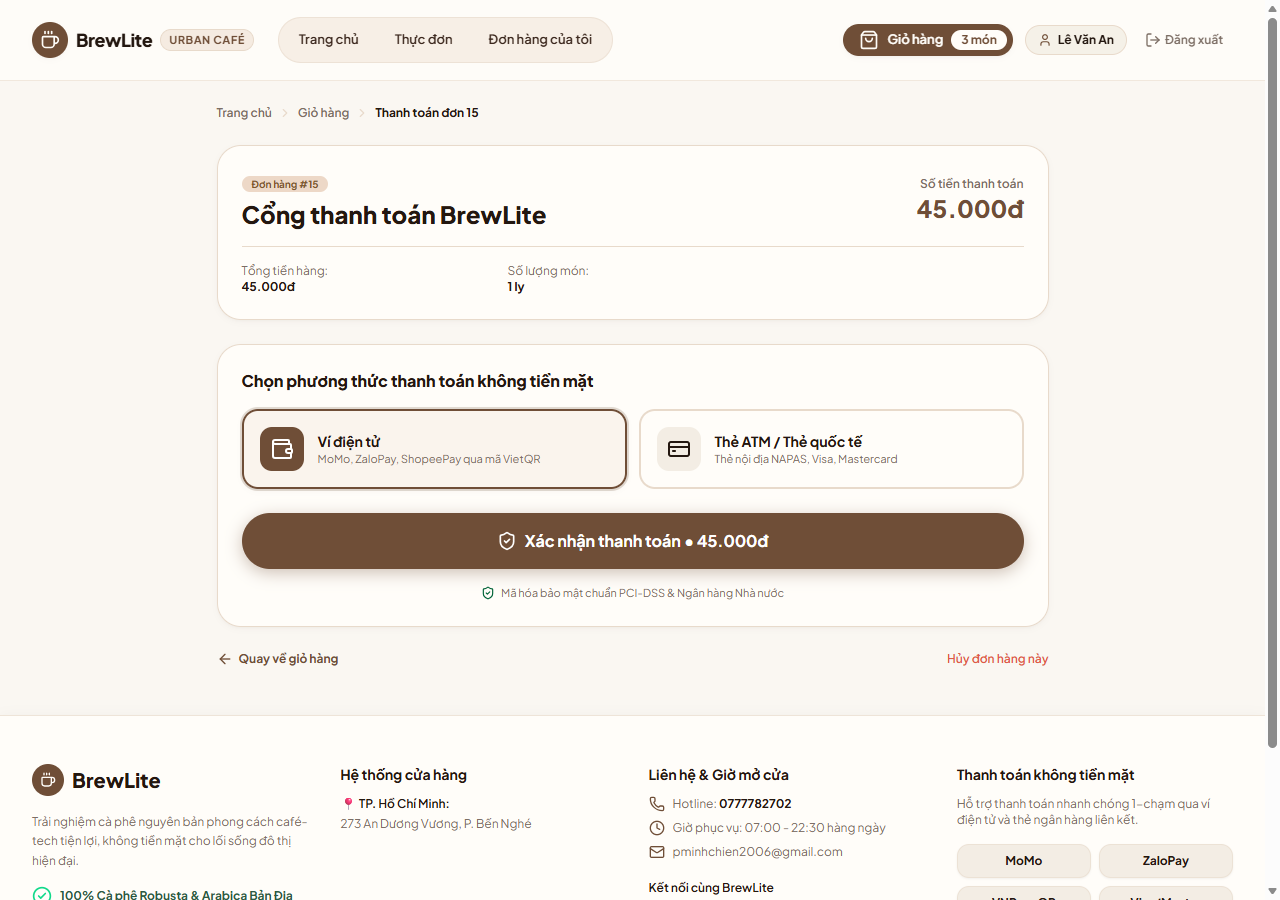
\includegraphics[width=0.92\textwidth]{figures/ui-payment.png}
    \caption{Giao diện Cổng thanh toán không tiền mặt đa phương thức}
    \label{fig:ui-payment}
\end{figure}

\section{Phân hệ Lịch sử Đơn hàng (Order History)}

\subsection{Đặc tả Use Case}
Phân hệ Lịch sử Đơn hàng cho phép khách hàng tra cứu toàn bộ các đơn hàng đã đặt trong quá khứ, theo dõi trạng thái pha chế và kiểm tra hóa đơn chi tiết. Sơ đồ Use Case được minh họa tại Hình~\ref{fig:usecase-order-history}.

\begin{figure}[htbp]
    \centering
    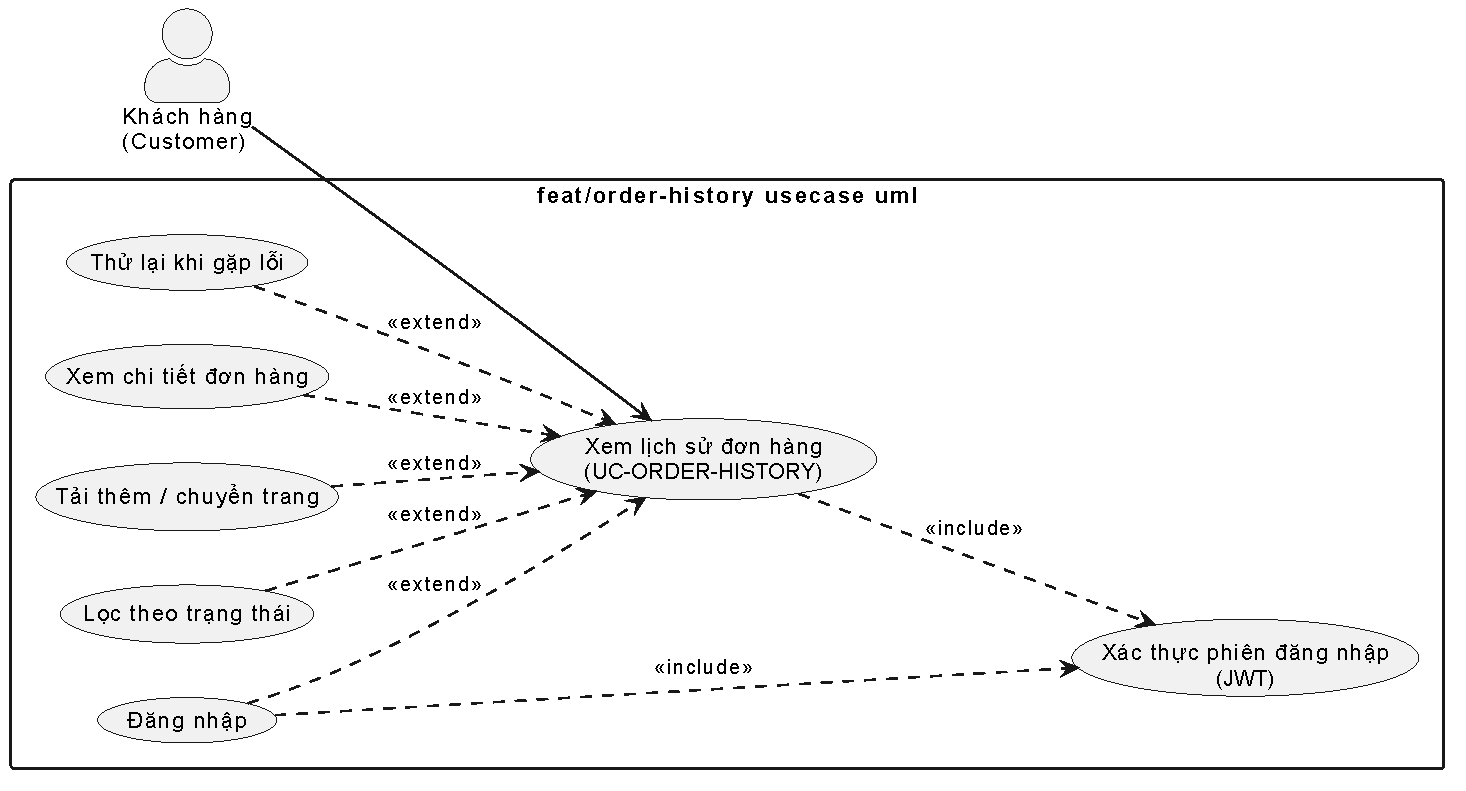
\includegraphics[width=0.75\textwidth]{figures/usecase-order-history.pdf}
    \caption{Sơ đồ Use Case - Phân hệ Lịch sử Đơn hàng}
    \label{fig:usecase-order-history}
\end{figure}

\begin{table}[htbp]
\centering
\small
\caption{Đặc tả Use Case: Tra cứu Lịch sử và Chi tiết Đơn hàng (UC-HIS-01)}
\label{tab:uc-spec-history}
\begin{tabularx}{\textwidth}{p{2.8cm}X}
\toprule
\textbf{Mục} & \textbf{Chi tiết Đặc tả} \\
\midrule
\textbf{Actor} & Khách hàng đã đăng nhập \\
\midrule
\textbf{Tiền điều kiện} & Khách hàng đã đăng nhập vào hệ thống. \\
\midrule
\textbf{Hậu điều kiện} & Danh sách các đơn hàng và trạng thái chi tiết hiển thị trực quan. \\
\midrule
\textbf{Luồng chính} & 
1. Khách hàng nhấp vào mục "Lịch sử đơn hàng" trên thanh điều hướng hoặc truy cập \texttt{/orders}.\newline
2. Giao diện gửi request \texttt{GET /api/v1/orders} kèm Bearer Token.\newline
3. Backend truy vấn các đơn hàng thuộc về \texttt{userId} hiện tại, sắp xếp giảm dần theo thời gian tạo (\texttt{createdAt desc}).\newline
4. Màn hình hiển thị danh sách các thẻ đơn hàng: mã hiển thị \texttt{\#orderNumber}, ngày giờ đặt, tổng tiền, huy hiệu trạng thái (ví dụ "Đã thanh toán", "Đã hủy").\newline
5. Khách hàng nhấp vào một đơn hàng để xem chi tiết hóa đơn (\texttt{/orders/[id]}): danh sách từng món, size, topping, số tiền giảm giá và phương thức thanh toán. \\
\midrule
\textbf{Luồng ngoại lệ} & 
- Người dùng chưa có đơn hàng nào: Giao diện hiển thị thông báo "Bạn chưa có đơn hàng nào" và nút liên kết "Bắt đầu đặt món".\newline
- Phiên đăng nhập hết hạn: Báo lỗi \texttt{401 Unauthorized}, tự động chuyển hướng về trang đăng nhập. \\
\bottomrule
\end{tabularx}
\end{table}

\subsection{Sơ đồ Hoạt động (Activity Diagram)}
Quy trình truy vấn danh sách và xem chi tiết trạng thái đơn hàng được thể hiện tại Hình~\ref{fig:activity-order-history}.

\begin{figure}[htbp]
    \centering
    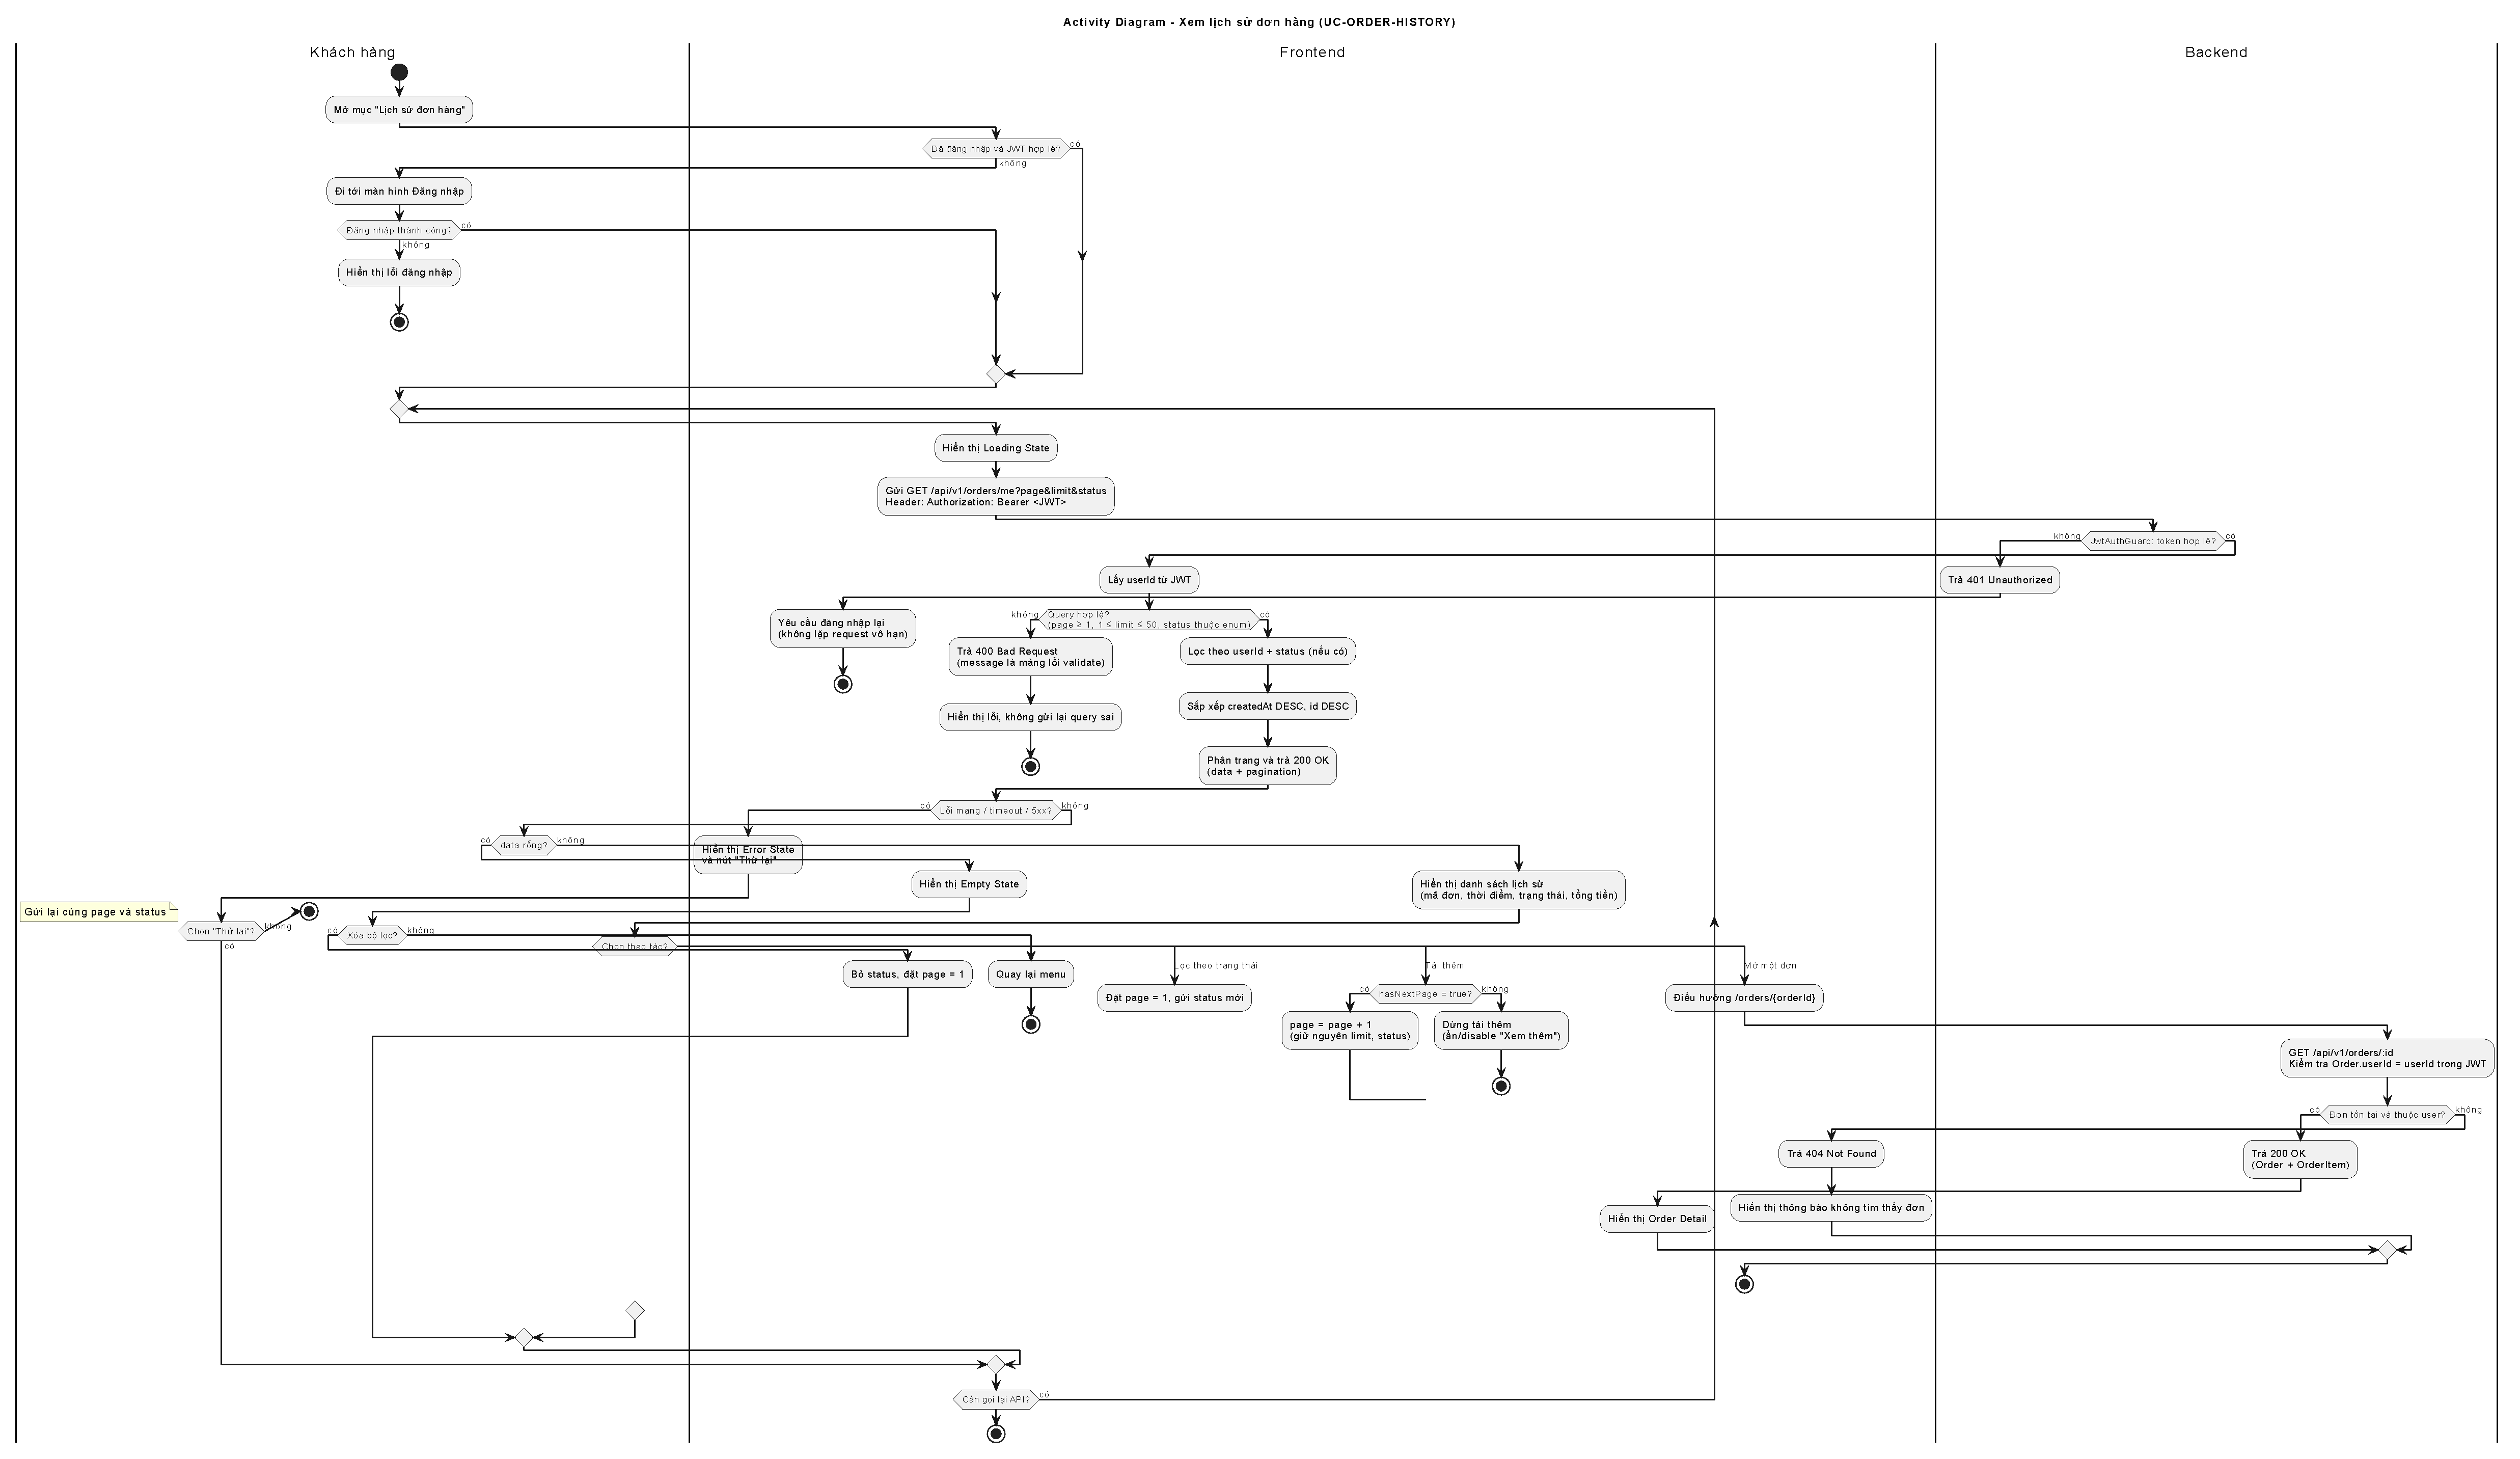
\includegraphics[width=0.75\textwidth]{figures/activity-order-history.pdf}
    \caption{Sơ đồ Hoạt động - Phân hệ Lịch sử Đơn hàng}
    \label{fig:activity-order-history}
\end{figure}

\subsection{Sơ đồ Tuần tự (Sequence Diagram)}
Sơ đồ Tuần tự minh họa tương tác nạp dữ liệu lịch sử đơn hàng từ Frontend đến Controller, Service và Prisma tại Hình~\ref{fig:sequence-order-history}.

\begin{figure}[htbp]
    \centering
    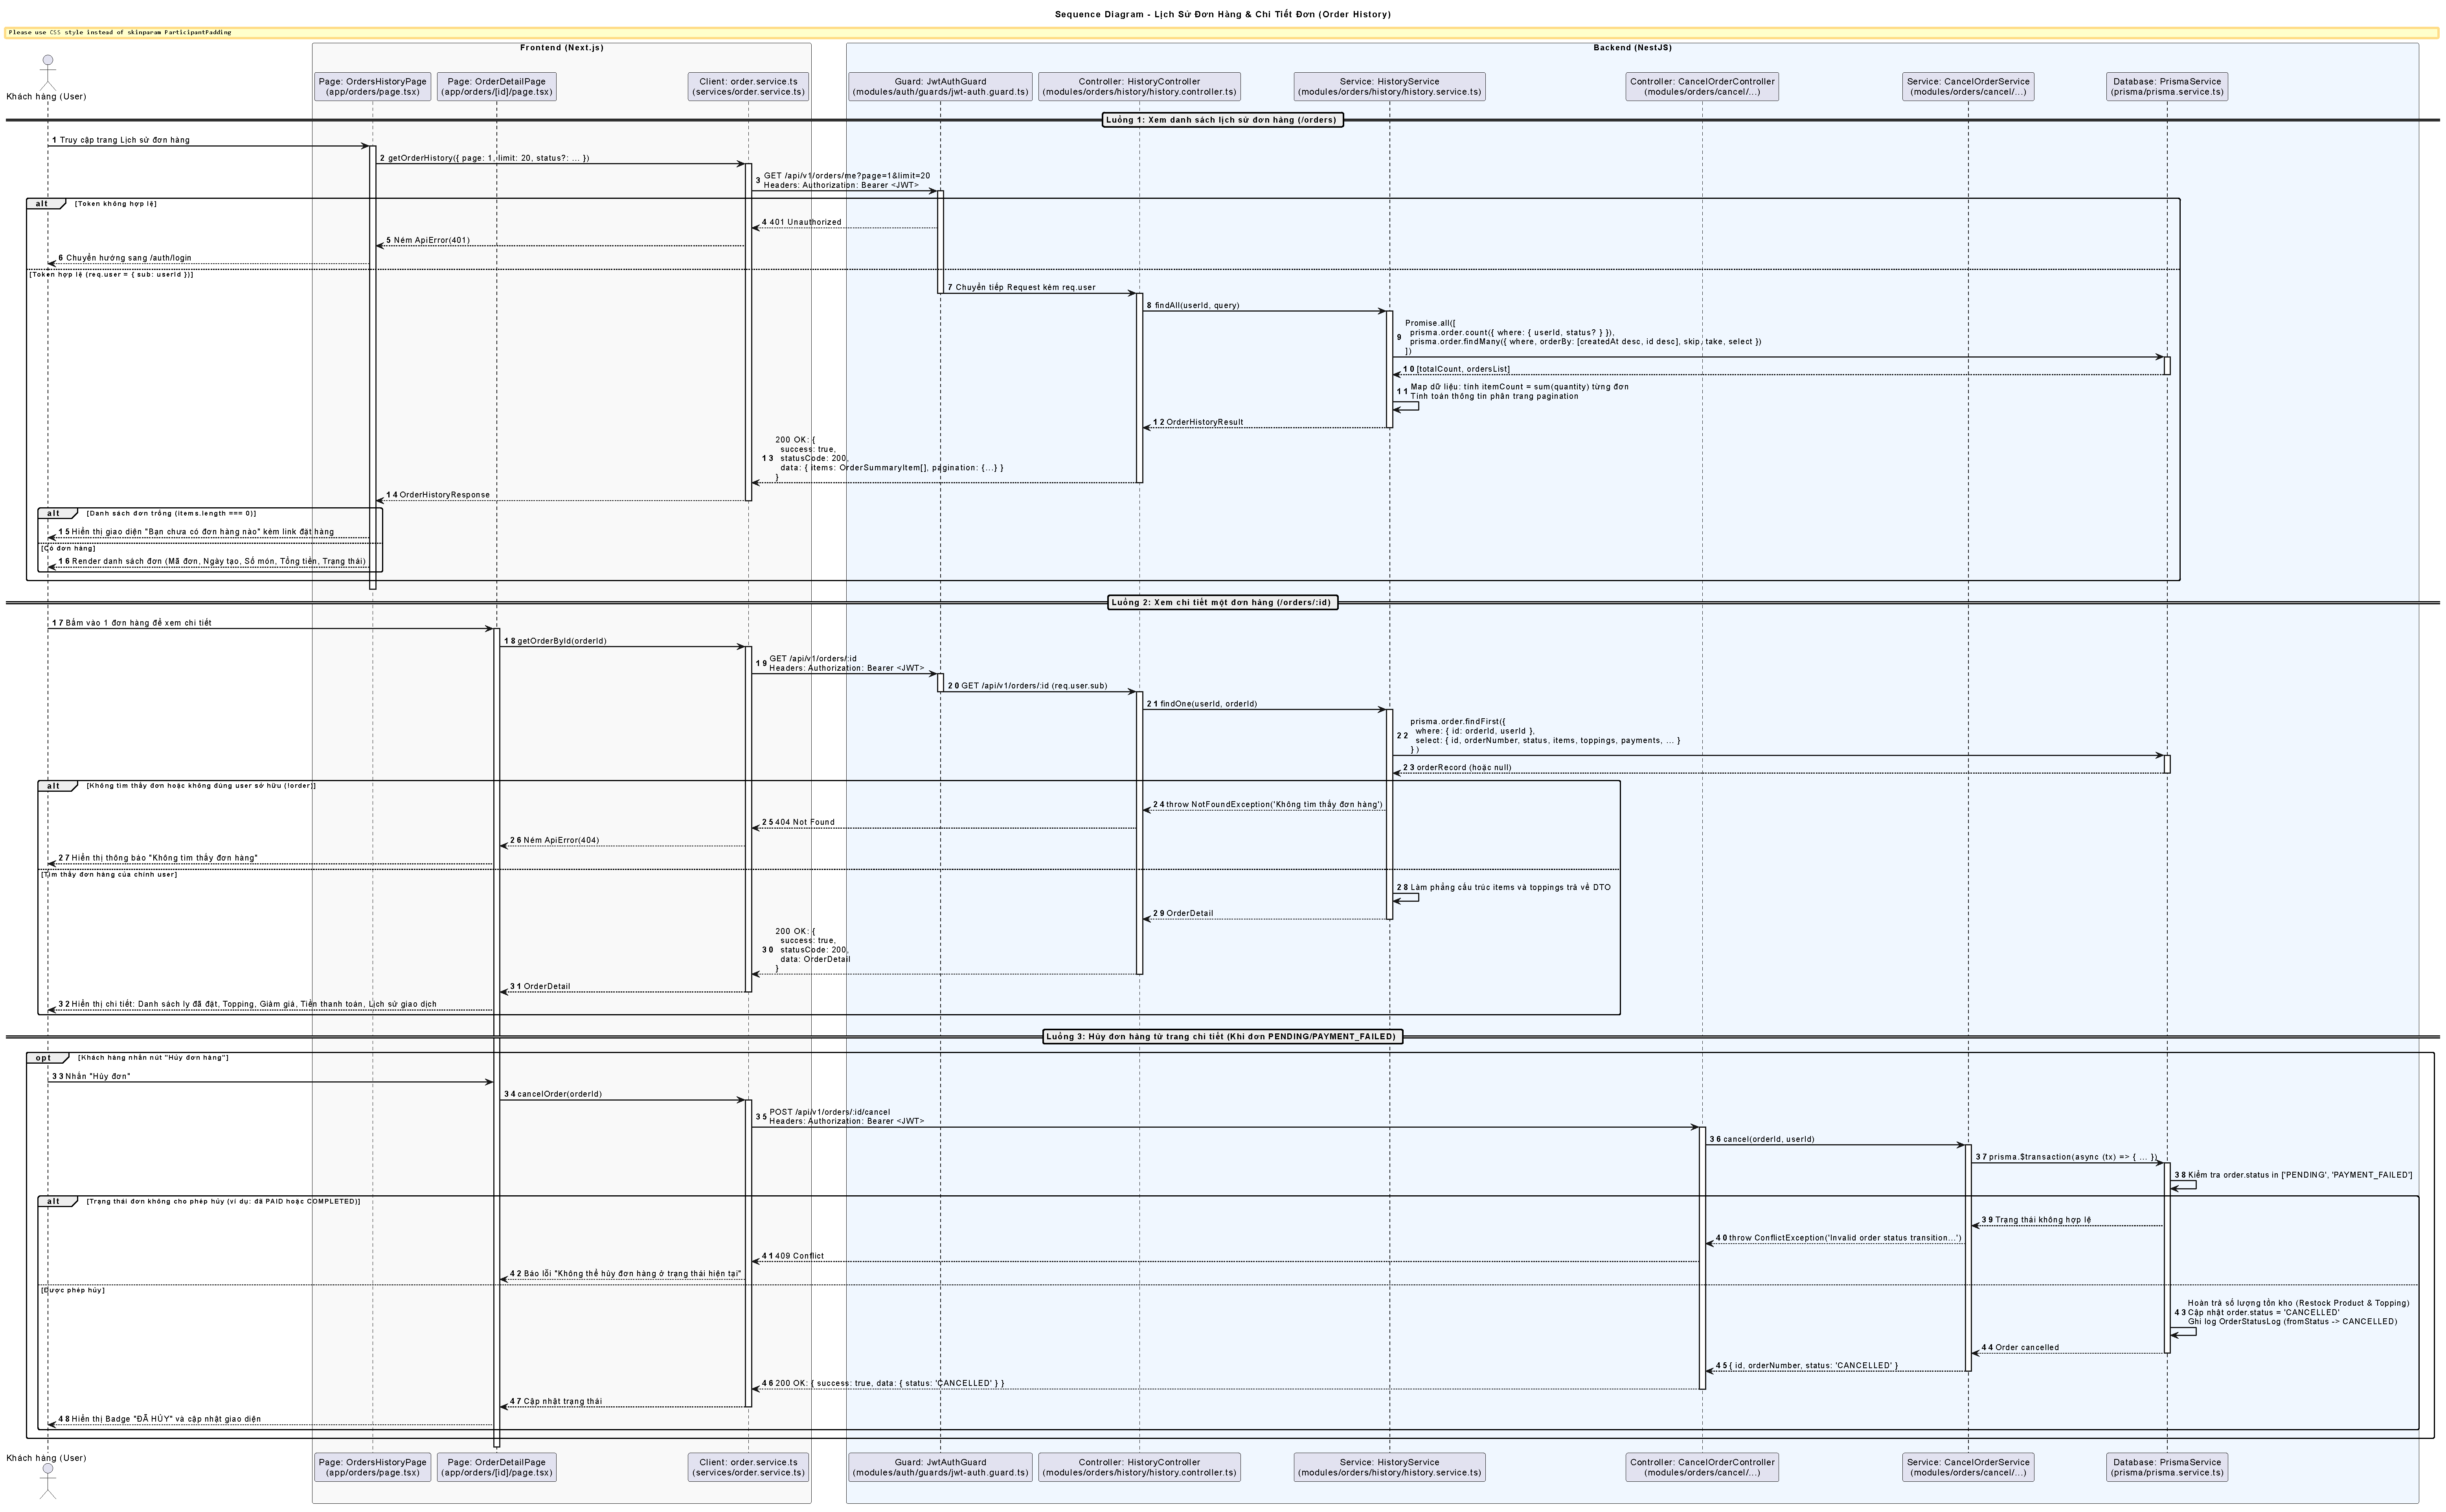
\includegraphics[width=0.9\textwidth]{figures/sequence-order-history.pdf}
    \caption{Sơ đồ Tuần tự - Phân hệ Lịch sử Đơn hàng}
    \label{fig:sequence-order-history}
\end{figure}

\subsection{Hợp đồng API (API Contract)}
\begin{table}[htbp]
\centering
\small
\caption{Danh mục API Endpoints - Phân hệ Lịch sử Đơn hàng}
\label{tab:api-history}
\begin{tabularx}{\textwidth}{llp{4cm}X}
\toprule
\textbf{Phương thức} & \textbf{Endpoint} & \textbf{Header} & \textbf{Phản hồi chính} \\
\midrule
\texttt{GET} & \texttt{/api/v1/orders} & \texttt{Authorization: Bearer <JWT>} & \texttt{200 OK}: Danh sách các đơn hàng của user đang đăng nhập, kèm tổng tiền và trạng thái. \\
\texttt{GET} & \texttt{/api/v1/orders/:id} & \texttt{Authorization: Bearer <JWT>} & \texttt{200 OK}: Chi tiết đơn hàng gồm các món (\texttt{items}), topping và lịch sử trạng thái (\texttt{statusHistory}). Lỗi \texttt{404} nếu không tìm thấy hoặc không thuộc sở hữu. \\
\bottomrule
\end{tabularx}
\end{table}

\subsection{Ánh xạ Cơ sở dữ liệu (Database Mapping)}
\begin{itemize}
    \item Truy vấn danh sách đơn hàng cá nhân:
    \begin{lstlisting}[language=SQL]
SELECT id, order_number, status, total_amount, discount_amount, final_amount, created_at 
FROM orders 
WHERE user_id = :userId 
ORDER BY created_at DESC;
    \end{lstlisting}
    \item Tối ưu hóa: Chỉ mục \texttt{@@index([userId])} và \texttt{@@index([status])} trên bảng \texttt{orders} đảm bảo câu truy vấn thực thi với độ phức tạp \(\mathcal{O}(\log N)\), đáp ứng yêu cầu phản hồi nhanh của hệ thống.
\end{itemize}

\subsection{Kịch bản Kiểm thử (Test Cases)}
\begin{table}[htbp]
\centering
\small
\caption{Tóm lược các Ca kiểm thử tiêu biểu - Phân hệ Lịch sử}
\label{tab:tc-history}
\begin{tabularx}{\textwidth}{llp{2.6cm}p{3cm}Xc}
\toprule
\textbf{Mã TC} & \textbf{Loại} & \textbf{Tiền điều kiện} & \textbf{Endpoint / Màn hình} & \textbf{Kết quả mong đợi} & \textbf{Trạng thái} \\
\midrule
\texttt{TC-HIS-API-01} & Hợp lệ & User có 3 đơn hàng & \texttt{GET /orders} & HTTP 200, trả về đủ 3 đơn sắp xếp mới nhất & Chưa chạy \\
\texttt{TC-HIS-API-02} & Bảo mật & Xem đơn của user khác & \texttt{GET /orders/:id} & HTTP 404 hoặc 403, không lộ đơn của người khác & Chưa chạy \\
\texttt{TC-HIS-UI-01} & Giao diện & User chưa có đơn nào & Màn hình \texttt{/orders} & Hiển thị chuỗi "Bạn chưa có đơn hàng nào" & Chưa chạy \\
\texttt{TC-HIS-UI-03} & Giao diện & Đơn đã bị hủy & Danh sách đơn & Hiển thị đúng badge trạng thái "Đã hủy" & Chưa chạy \\
\bottomrule
\end{tabularx}
\end{table}

\subsection{Giao diện Người dùng}
\begin{figure}[htbp]
    \centering
    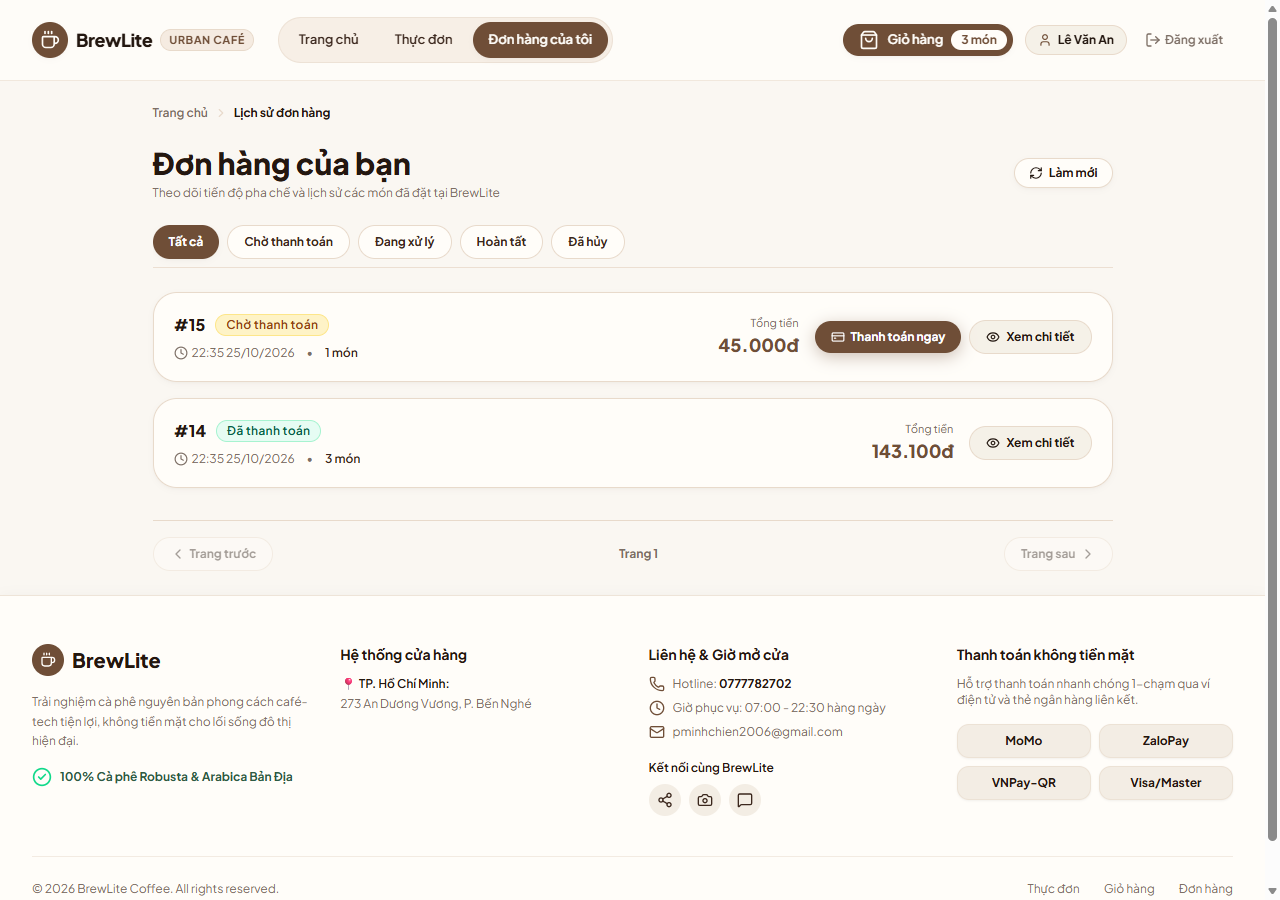
\includegraphics[width=0.92\textwidth]{figures/ui-history.png}
    \caption{Giao diện Lịch sử và Trạng thái Đơn hàng của Khách hàng}
    \label{fig:ui-history}
\end{figure}

